\documentclass{article}
\usepackage[utf8]{inputenc}
\usepackage{palatino} %font type
\usepackage{tikz}
\usepackage{amsmath}
\usepackage{enumitem,amssymb, gensymb}
\usepackage{graphicx}
\usepackage{caption}
\usepackage{subcaption}
\usepackage{tabularx}
\usepackage[table]{xcolor}
\usepackage{booktabs}
\usepackage{fancyhdr}
\usepackage[export]{adjustbox}


\graphicspath{ {./images/} }
\usepackage[
backend=biber,
style=apa]{biblatex}
\linespread{2}

\addbibresource{ref.txt}

\title{Characterising Temporal Dynamics of Visual Perceptual Grouping}
\author{Mehmet Yörüten}
\date{\today}

% Set up the caption sizes
\captionsetup{font={small,stretch=1.3}}


% Set up the headers
\pagestyle{fancy}
\fancyhf{} % clear all header and footer fields
\renewcommand{\headrulewidth}{0pt}
\fancyhead[L]{TEMPORAL DYNAMICS OF VISUAL GROUPING} % add running title to the left header
\rhead{\thepage} % add page number to the center footer


\fancypagestyle{firstpage}{
  \fancyhf{}
  \fancyhead[L]{Running head: TEMPORAL DYNAMICS OF VISUAL GROUPING} % add running title to the left header
  \rhead{\thepage} % add page number to the center footer
}


\begin{document}

%\maketitle
%\thispagestyle{firstpage}
\clearpage

\section*{Acknowledgments}
I would like to express my heartfelt gratitude to Shuchen Wu for her unwavering support and supervision throughout the writing of my thesis. Her invaluable advice, ideas, moral support, and patience were instrumental in guiding me through this project. I feel incredibly lucky to have had such an amazing supervisor.

I am also extremely grateful to Dr. Eric Schulz, who created the welcoming environment of Computational Principles of Intelligence Lab. His mentorship and support were critical in helping me grow as a researcher and a person. I could not have imagined a better place to undertake this journey.

In addition, I would like to thank Professor Felix Wichmann and Dr. Uli Wanek for their generosity in allowing us to use their lab and for sharing their expertise and knowledge. Their continuous guidance and support kept me motivated throughout the writing of this thesis.

Finally, I would like to express my appreciation to David Elias Künstle for his assistance and for administering the use of the room. 
\clearpage

\section{Abstract}
When you glimpse mountainous scenery, you perceive the rough shape of the scene. Taking a closer look, you would discover intricate details about regions of bushes and rocks of diverse species. We are exceptionally good at perceiving an image as parts and wholes. How does perceptual grouping behavior change with an increasing level of exposure time? And what would be a model to describe this process? While previous studies have suggested the precedence of global over local grouping, how the granularity of image segmentation changes with increasing exposure time remains elusive.
We propose a novel paradigm to study the relationship between visual perceptual grouping with exposure times. We relate the exposure time to computational resources attributed to image segmentation in the normalized min-cut algorithm. This method transfers an image segmentation problem into a graph-cutting problem, thus enabling us to connect computational resources (cut level) with the precedence of perceptual grouping. This allows us to produce image segmentation of various cut levels to probe subjects’ recognition behavior at different exposure times. Thereby testing the prediction that perceptual grouping goes from coarse to fine with more computational resources. Our findings show that sensitivities to finer parts of the images increase with longer exposure to the image.

\clearpage

\tableofcontents

\clearpage

\section{Introduction}
Visual perception starts with the activation of individual photoreceptors in the retina. However, our visual experience is not complex as much as the individual workings of these neurons. Instead, our visual perception effectively organizes the world around us into parts with meaningful relations to each other. Visual scenes would appear disorderly in the absence of any structure or organization. Perceptual organization refers to the structural relationship between these parts which form meaningful and consistent visual experiences.

\subsection{Visual Perceptual Grouping}
This organizational problem has many possible solutions. To interpret which visual elements are more likely to be organized together, grouping principles were offered by Gestalt Psychologists (e.g., \cite{wertheimer1923brief}). These principles are closely associated with the perceptual organization, and they draw attention to the features of visual elements. They include similarity, good continuation, closure, proximity, and common fate (Figure \ref{fig:GestaltPrincips}). According to the similarity principle, given the fact that all other features of visual elements are equal, the ones carrying the same distinct properties in color, size, or orientation are grouped together. \citeauthor{wertheimer1923brief} also suggests that good continuation refers to the tendency to group visual elements following smooth, continuous lines and patterns (\citeyear{wertheimer1923brief}). Closure occurs when grouping happens in enclosed regions. Proximity refers to the tendency to group the visual elements which are placed close to each other. Lastly, common fate describes the tendency to group elements that move in the same direction.

\begin{figure}[h!]
    \centering
    \begin{subfigure}{0.47\textwidth}
        \centering
        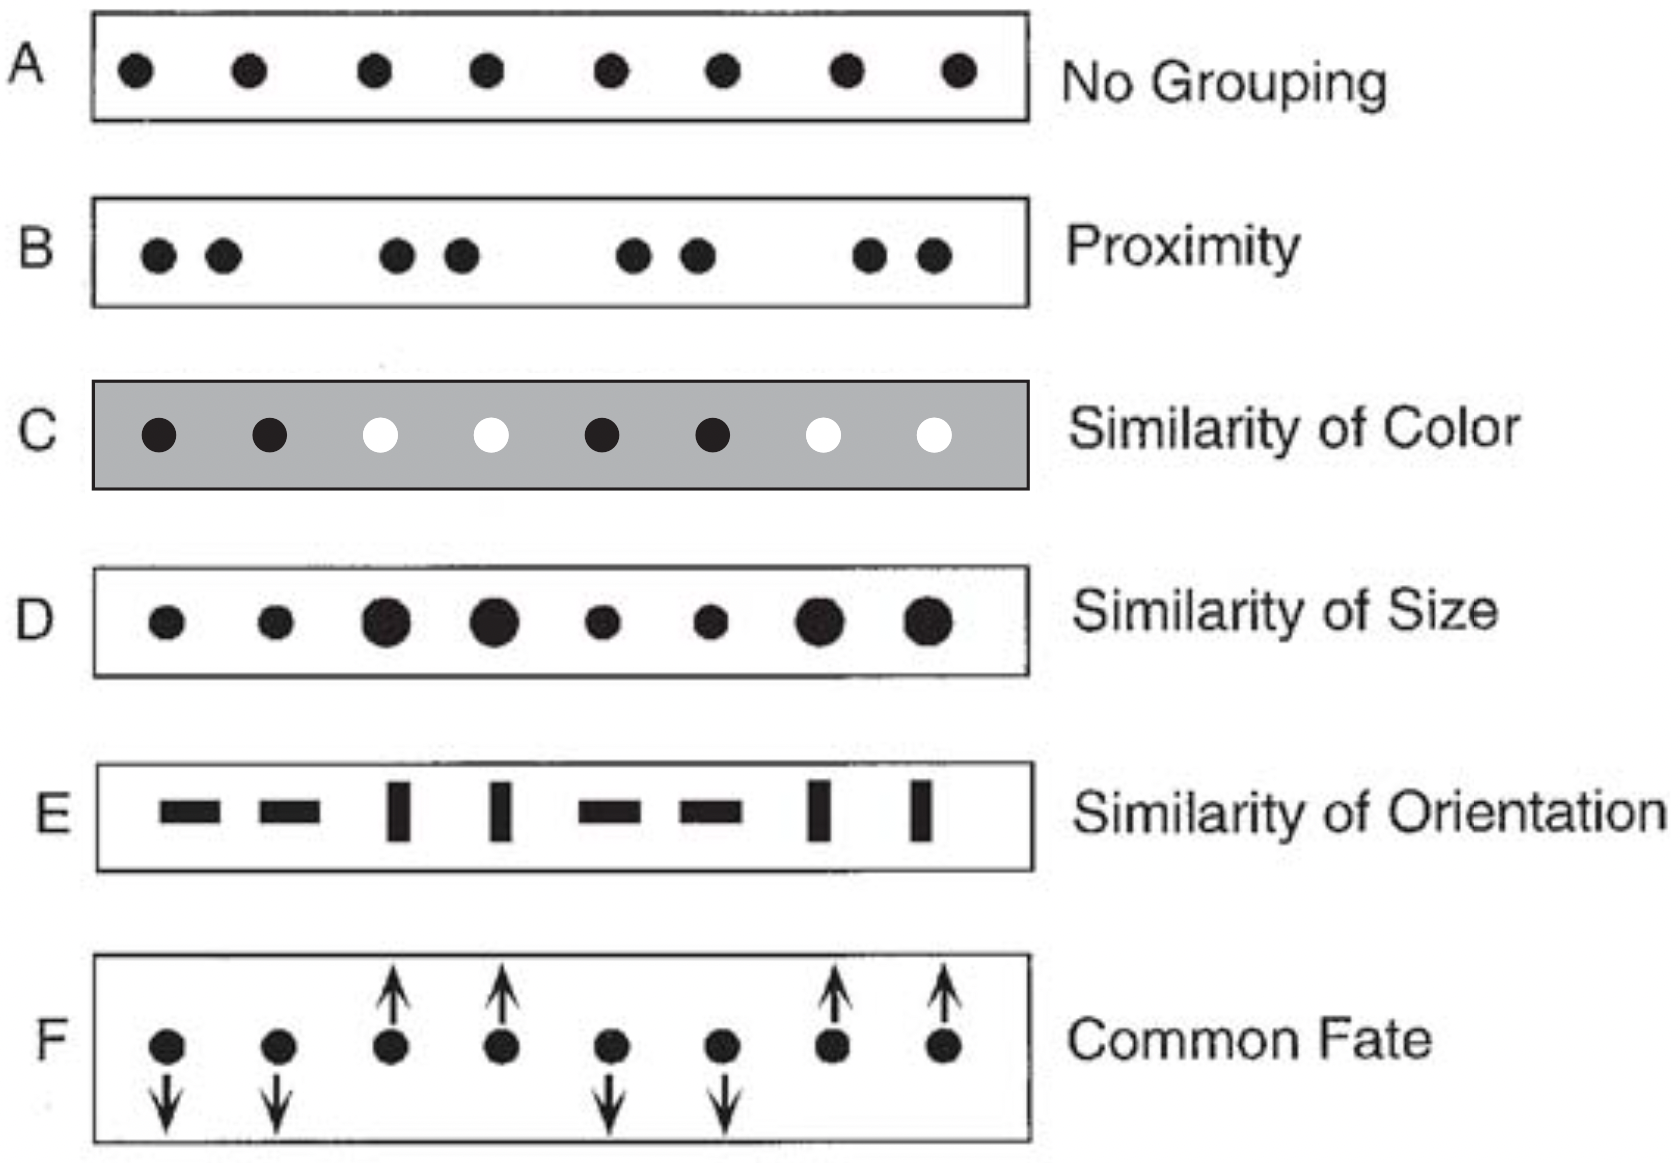
\includegraphics[width=\textwidth]{Thesis/images/gestaltPrinciples.png}
        \label{figure:Gestalt1}
    \end{subfigure}
    \hfill
    \begin{subfigure}{0.47\textwidth}
        \centering
        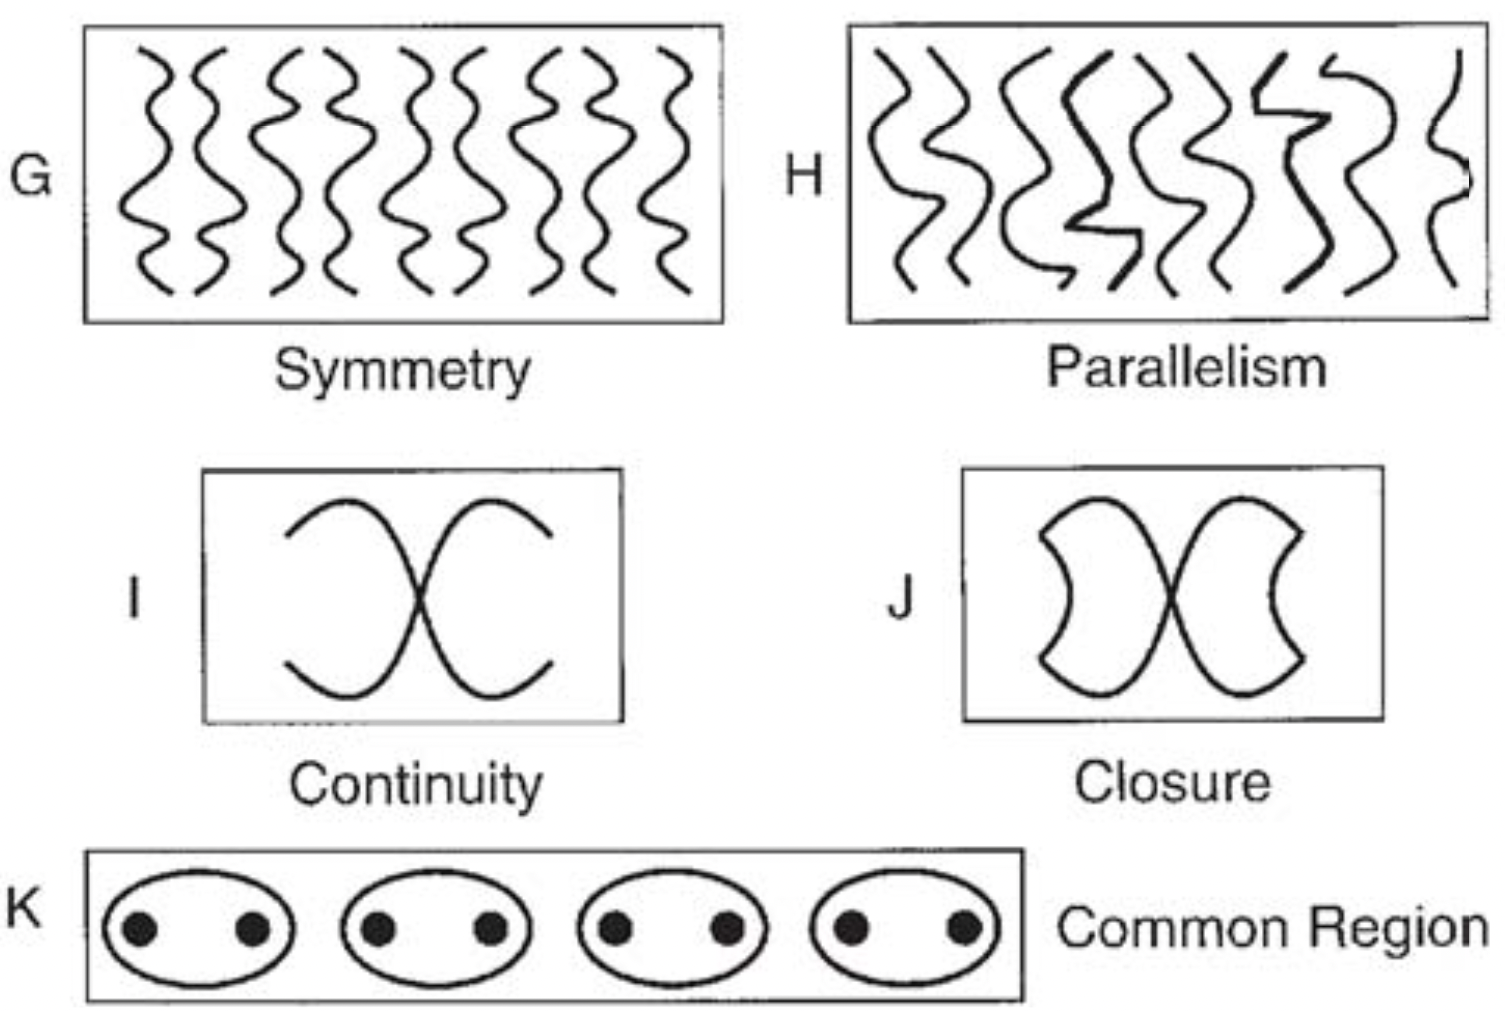
\includegraphics[width=\textwidth]{Thesis/images/gestaltPrinciples2.png}
        \label{figure:Gestalt2}
    \end{subfigure}
    \hfill
    \caption{Some Gestalt Principles describing the way we assemble the elements into groups. Adapted by {\cite{RN212}}.}
    \label{fig:GestaltPrincips}
\end{figure}

This grouping behavior can be executed rapidly even under inattention (\cite{RN192}; \cite{RN207}). However, there are temporal limitations to this behavior (\cite{RN228}; \cite{RN233}; \cite{RN225}). Although the grouping can occur with the presentation of two successive stimuli which complete each other (\cite{RN233}), the time range of grouping is not generous and general to all the grouping principles (\cite{RN228}). \citeauthor{RN228}, in their study, presented a mask after a grouped set of stimuli. Depending on the temporal differences between the presentations, they showed that masks can interfere with the grouping behavior. More interestingly, the temporal property of the interference was dependent on the type of grouping. Mean interference of the mask occurred earlier when the presented stimuli had grouping with alignment, in comparison to the grouping with proximity. These results suggest that more time is needed to group when the grouping is performed with an alignment cue. However, the difference between these two processes could be due to the fact that alignment is not a very well-established grouping principle.

There is also some research done to test the effect of time course on similarity by achromatic color (\cite{RN234}). In this experiment, the authors wanted to understand if grouping happens in early or late vision. To test this idea, they designed a paradigm in which 5 columns of grey squares were presented. Two of the columns had darker grey than the rest of the columns. By casting a shadow onto the central column, its luminance  was matched with the darker grey columns. In the end, they had a stimulus which have the same reflectance values for the columns in one direction and the same luminance as the ones in the other direction. Results showed that their participants grouped the stimuli depending on their reflectance properties suggesting that grouping by achromatic similarity happens not at the retinal level but at the later phases of the vision. However, another research conducted by \citeauthor{RN229} using the same method but with chromatic stimuli proved that grouping with similarity by color can occur both in early and late vision (\citeyear{RN229}). While the grouping with luminance properties happened when the stimuli were presented for 200 ms, grouping with reflectance was dominant when the exposure time is 2000 ms. Furthermore, different types of visual information can be accessed at different exposure times (\cite{RN235}).  

Grouping principles are not the only defining factors of perceptual organizations. Previous studies have suggested that the grouping of global features takes precedence over the grouping of local features (\cite{RN196}; \cite{RN194}). Global precedence phenomena show that global aspects of a visual scene are processed more rapidly than its local features. Although the presentation time did not show an effect on global precedence (\cite{luna1995selective}; \cite{luna1993effects}), it can interact with the features of the stimuli like the angle of the local elements and diminish the effect (\cite{luna1995selective}). Therefore, understanding the temporal dynamics of grouping behavior and global precedence phenomena requires further investigation considering its interaction with the stimulus features. 

Although intensive research was conducted on perceptual grouping, the studies were limited by two levels of hierarchy (\cite{RN195};  \cite{RN191};  \cite{RN232}). For instance, while \citeauthor{RN196} was testing global precedence phenomenon, he used large letters composed of smaller ones (\citeyear{RN196}). After presenting these letters for 150 ms, participants needed to respond to auditory stimuli by pronouncing either local (smaller) or global (larger) letter was used (\cite{stroop1935studies}). Results showed that participants reacted to local letters slower than  global letters. It was also shown that they were prone to do more mistakes when local letters were tested. In another experiment, horizontal or vertical lines were used rather than using letters (\cite{RN232}). In their task, horizontal or vertical clusters were formed with smaller lines inside them. These clusters (global feature) were either congruent or incongruent with the orientations of the lines (local feature) forming them. Between-group comparisons showed that participants who needed to respond to local orientations were slower in comparison to the group responding to global orientations. Another research done with biological motion showed that by using only 10 to 12 elements of moving dots it is possible to demonstrate human walking pattern (\cite{johansson1973visual}). This perceptual experience highlights a similar phenomenon to grouping principles by embracing the idea of the whole is greater than the summation of its parts. 

On the other hand, some recent works suggest that some hierarchical order with more than two levels can be established. It was shown how moving scenes can be partitioned into finer elements using the Bayesian framework (\cite{RN177}). Another research done by \citeauthor{hafri_green_firestone_2023} speculates that we can understand the relationships between objects by identifying shared features, leading to a compositional view of visual perception similar to the linguistic models (\citeyear{hafri_green_firestone_2023}). However, despite these high-level insights, it remains crucial to understand the low-level mechanisms underlying visual perception through psychophysical approaches. Moreover, while these theories suggest that hierarchical structure  does not require to be composed only of two levels (\cite{RN236}; \cite{RN177}), they should be tested with human participants to find behavioral basis. Since the current experimental paradigms do not offer a chance to test hierarchy with more than two levels, it is necessary to design a new stimulus. Therefore, we introduce novel stimuli which can be tested at different levels of the hierarchy. 

Lastly, a model which can approximate the relationships between perceptual grouping,  exposure time, and level of segmentation is missing. If there is a hierarchical order in segmenting visual scenes in our perceptual behavior, a working model should perform this behavior in the same order. While doing so, it should also preserve the relationships between elements defined by Gestalt principles. The model should also have means to represent the computational resources spent on the segmentation process.


\subsection{Modeling Perceptual Grouping}
The normalized min-cut algorithm is one of the image segmentation algorithms which fulfills the listed conditions (\cite{RN165}). Their approach attempts to solve the image segmentation problem by transforming images into graphs where each pixel represents a node. By considering the feature properties of these pixels and their spatial distances, their algorithm performs partitioning which is also known as cut in graph theory terminology. The similarity of this algorithm to human grouping behavior derives from the fact that it employs properties of grouping principles to perform segmentation. Thanks to graph theory's consideration of these properties, the algorithm prioritizes some elements in the graph over others. By assigning high weights between similar regions in a graph, the normalized min-cut algorithm exhibits similar grouping behavior defined by Gestalt principles. Graph theory is also shown as an efficient method for solving complex structures (\cite{newman2003structure}). Since grouping behavior occurs rapidly and in a consistent manner although it is a complex process, it can be contended that the efficiency of the normalized min-cut algorithm can be adapted to this process. Additionally, the algorithm recursively cuts the given image into two parts at each step and provides us with a numeric value corresponding to the difficulty of partitioning. Thus, the normalized min-cut algorithm administers a hierarchy in an image with the numeric values that we are seeking.

\subsection{Our Study}
Our research focuses on several important gaps in this line of study. First, considering our cognitive resources are limited (\cite{baddeley1974working}; \cite{hertwig2003coglimit}; \cite{phillips1977vismem}), segmentation of complex visual scenes should not be independent of presentation duration. In this thesis, we propose a novel paradigm to study the relationship between visual perceptual grouping and exposure time. By using the normalized min-cut algorithm, we are able to connect computational resources to the precedence of perceptual grouping and produce image segmentations at different levels of granularity. This allows us to test the hypothesis that perceptual grouping becomes increasingly fine-grained with more computational resources and longer exposure times (Figure \ref{fig:hypothesis}). Through our experiments, we aim to contribute to a deeper understanding of the mechanisms underlying visual perception. 


To do so we developed a novel experimental paradigm that we presented images which were generated using hexagons. Since we modulated the intensities of these hexagons, it was possible to perceive 6 different segments when the unlimited time was given. These segments were later retrieved by the normalized min-cut algorithm and presented either for a short or long periods of time. Since the algorithm cuts the image into smaller parts in a recursive fashion, we could assign an order to found segments. This method helped us to tackle the problem of testing hierarchy with more than two levels. By asking participants to detect if the presented segment had been a part of the image, we were able to test participant performance for hierarchical grouping ability and for different exposure time conditions. 

Our results showed that participants struggled to detect the segments with higher cut no. It suggests that they had difficulty in identifying the parts of an image that were partitioned later, as opposed to those partitioned earlier. We also observed that exposure time had a notable impact on performance. These findings suggest that hierarchical grouping performance can be approximated by the normalized min-cut algorithm. Furthermore, when more computational resources are available to participants they are better at partitioning an image into finer parts. 

\begin{figure}
    \centering
    \hspace*{-0.85cm} 
    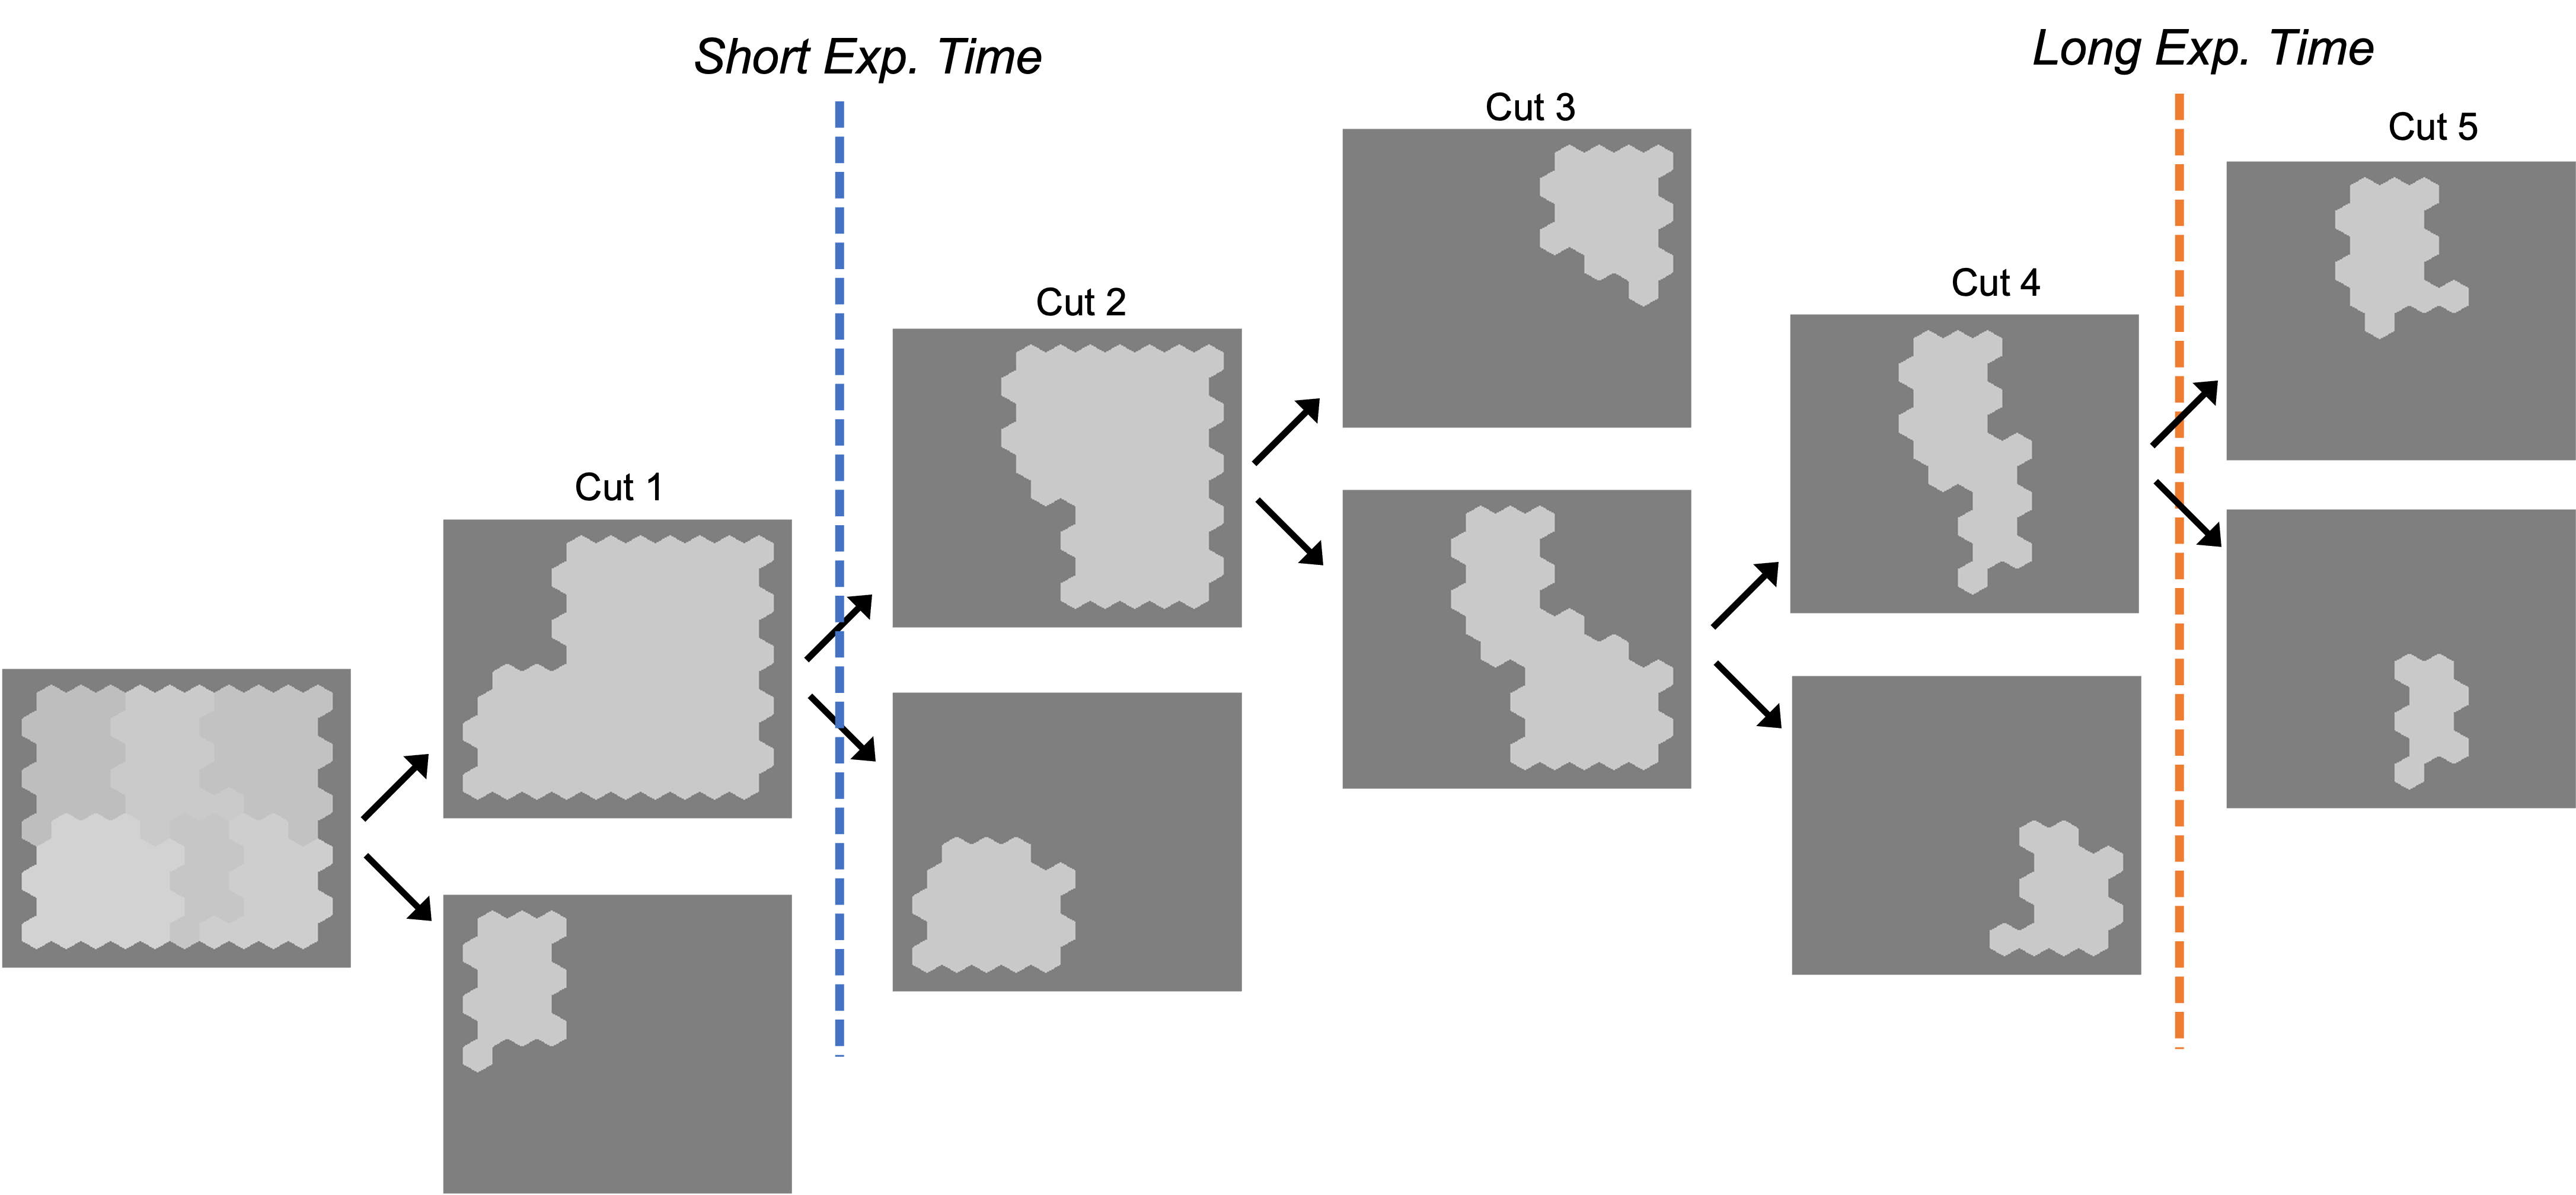
\includegraphics[width=1.2\textwidth]{figs/segmentation_example.png}
    \caption{An example partitioning process. Blue and red dotted lines highlight the hypothesized limit of human segmentation performance for short and long exposure times respectively. As more cognitive resources are available through the longer exposure time, we predicted that participants should be able to perform more steps of segmentation and show higher performance for the segments at higher cut levels.}
    \label{fig:hypothesis}
\end{figure}

The research has significant implications for both cognitive and computer scientists. Cognitive scientists can use the findings to study how the structure of perceptual grouping is related to factors like hierarchy and exposure time, even in the absence of any inductive bias. As perceptual grouping is a well-established characteristic of human vision, computer scientists can develop computer vision systems while considering these properties.


\section{Methods}
\subsection{Image Segmentation} \label{imageSegmentation}
To extract the segments from the image and compare human performance with a model, we used the normalized min-cut algorithm (\cite{RN165}). Normalized min-cut is an image segmentation algorithm which fulfills the listed conditions. It uses graph theory and eigendecomposition to partition the images. It recursively cuts the given image into two parts at each step, and it provides a numeric value corresponding to the difficulty of partitioning. 

\begin{figure}[!ht]
    \centering
    \begin{subfigure}[t]{0.32\textwidth}
        \centering
        \begin{tikzpicture}[node distance={2mm},  scale=5.1, every square/.style={regular polygon,regular polygon sides=4}, transform shape]
        
        \node(1) [fill=grey!10, square, fill];
        \node[main] (2) [fill=grey!10, square, fill, below of=1]; 
        \node[main] (3) [fill=grey!14, square, fill, below of=2];
        \node[main] (4) [fill=grey!23, square, fill, right of=1]; 
        \node[main] (5) [fill=grey!25, square, fill, below of=4];
        \node[main] (6) [fill=grey!45, square, fill, below of=5];
        \node[main] (7) [fill=grey!45, square, fill, right of=4]; 
        \node[main] (8) [fill=grey!45, square, fill, below of=7];
        \node[main] (9) [fill=grey!45, square, fill, below of=8];                                 
        \end{tikzpicture}    
    \caption{Example image to be segmented}
    \end{subfigure}
    \hfill
    \begin{subfigure}[t]{0.32\textwidth}           
        \centering
        \begin{tikzpicture}[node distance={8mm},  scale=1.5, thick, every square/.style={regular polygon,regular polygon sides=4}, transform shape]
        
        \node(1) [fill=grey!10, square, draw] {$v_1$};
        \node[main] (2) [fill=grey!10, square, draw, below of=1] {$v_2$}; 
        \node[main] (3) [fill=grey!14, square, draw, below of=2] {$v_3$};
        \node[main] (4) [fill=grey!23, square, draw, right of=1] {$v_4$}; 
        \node[main] (5) [fill=grey!25, square, draw, below of=4] {$v_5$};
        \node[main] (6) [fill=grey!45, square, draw, below of=5] {$v_6$};
        \node[main] (7) [fill=grey!45, square, draw, right of=4] {$v_7$}; 
        \node[main] (8) [fill=grey!45, square, draw, below of=7] {$v_8$};
        \node[main] (9) [fill=grey!45, square, draw, below of=8] {$v_9$};                
        \end{tikzpicture}        
    \caption{Representation of image with nodes}
    \end{subfigure}
    \hfill
    \begin{subfigure}[t]{0.32\textwidth}    
        \centering
        \begin{tikzpicture}[node distance={8mm},  scale=1.5, thick, every square/.style={regular polygon,regular polygon sides=4}, transform shape]
        
        \node(1) [fill=grey!10, square, draw] {$v_1$};
        \node[main] (2) [fill=grey!10, square, draw, below of=1] {$v_2$}; 
        \node[main] (3) [fill=grey!14, square, draw, below of=2] {$v_3$};
        \node[main] (4) [fill=grey!23, square, draw, right of=1] {$v_4$}; 
        \node[main] (5) [fill=grey!25, square, draw, below of=4] {$v_5$};
        \node[main] (6) [fill=grey!45, square, draw, below of=5] {$v_6$};
        \node[main] (7) [fill=grey!45, square, draw, right of=4] {$v_7$}; 
        \node[main] (8) [fill=grey!45, square, draw, below of=7] {$v_8$};
        \node[main] (9) [fill=grey!45, square, draw, below of=8] {$v_9$};        

        \path (3) edge (6)
                  (4) edge [bend right=45] (6)
                  (4) edge (7)
                  (5) edge (6)
                  (5) edge (8)
    
                  (1) edge [bend left=45] (7)
                  (2) edge [bend left=45] (8)
                  (3) edge [bend left=45] (9);
            
        \path[line width = 1.5pt]
              (1) edge (4)
              (2) edge (5)
              (2) edge (3);
              
        \path[line width = 2.5pt] 
              (1) edge (2)
              (1) edge [bend right=45] (3)
              (2) edge (3)
              (6) edge (9)
              (7) edge (8)
              (7) edge [bend right=45] (9)
              (8) edge (9)
              (4) edge (5);       
        \end{tikzpicture}        
    \caption{Assigning weights to the edges between nodes}
    \end{subfigure}
    
    %\bigskip % more vertical separation
    
   
    \centering
    \begin{subfigure}{0.3\textwidth}       
        \centering
        \begin{tikzpicture}[node distance={8mm},  scale=1.5, thick, every square/.style={regular polygon,regular polygon sides=4}, transform shape]
            \node(1) [fill=grey!10, square, draw] {$v_1$};
            \node[main] (2) [fill=grey!10, square, draw, below of=1] {$v_2$}; 
            \node[main] (3) [fill=grey!14, square, draw, below of=2] {$v_3$};
            \node[main] (4) [fill=grey!23, square, draw, right of=1] {$v_4$}; 
            \node[main] (5) [fill=grey!25, square, draw, below of=4] {$v_5$};
            \node[main] (6) [fill=grey!45, square, draw, below of=5] {$v_6$};
            \node[main] (7) [fill=grey!45, square, draw, right of=4] {$v_7$}; 
            \node[main] (8) [fill=grey!45, square, draw, below of=7] {$v_8$};
            \node[main] (9) [fill=grey!45, square, draw, below of=8] {$v_9$}; 
            
        \path[line width = 2pt] 
              (1) edge (2)
              (1) edge [bend right=45] (3)
              (2) edge (3)
              (4) edge (5)
              (7) edge (8)
              (8) edge (9)
              (6) edge (9);

        \path[line width = 1.5pt] 
              (1) edge (4)
              (2) edge (5);
                                            
        \end{tikzpicture}
    \caption{Graph after the first cut}     
    \end{subfigure}
    \hspace{0.05\textwidth}
    \begin{subfigure}{0.3\textwidth}   
        \centering
        \begin{tikzpicture}[node distance={8mm},  scale=1.5, thick, every square/.style={regular polygon,regular polygon sides=4}, transform shape] 
    
        \node(1) [fill=grey!10, square, draw] {$v_1$};
        \node[main] (2) [fill=grey!10, square, draw, below of=1] {$v_2$}; 
        \node[main] (3) [fill=grey!14, square, draw, below of=2] {$v_3$};
        \node[main] (4) [fill=grey!23, square, draw, right of=1] {$v_4$}; 
        \node[main] (5) [fill=grey!25, square, draw, below of=4] {$v_5$};
        \node[main] (6) [fill=grey!45, square, draw, below of=5] {$v_6$};
        \node[main] (7) [fill=grey!45, square, draw, right of=4] {$v_7$}; 
        \node[main] (8) [fill=grey!45, square, draw, below of=7] {$v_8$};
        \node[main] (9) [fill=grey!45, square, draw, below of=8] {$v_9$};     
            
            \path[line width = 2.5pt] (1) edge (2)
                  (2) edge (3)
                  (4) edge (5)
                  
                  (7) edge (8)
                  (8) edge (9)
                  (6) edge (9)              
        \end{tikzpicture}
    \caption{Graph after the second cut}
    \end{subfigure}
    
    \caption{Steps illustrating the image segmentation procedure using the normalized min-cut algorithm. The pixels in the image are first represented as nodes in a graph (\textbf{a.} and \textbf{b.}), and edges are assigned weights based on their intensity similarities (\textbf{c.}). The graph is then cut into segments that are most dissimilar to each other (\textbf{d.} and \textbf{e.}). This procedure continues recursively until all the segments found in the image.}
    \label{fig:img_as_grph}
\end{figure}


In the first step, we transform an image segmentation problem into a graph cutting problem (Figure \ref{fig:img_as_grph}). To this end, we represented the displayed image via a weighted graph. This weighted graph $G = (V,E)$ was generated by representing hexagons as nodes. The weights of this graph were computed using the normalized intensity values $F$ and the locations $X$ of the nodes. When hexagons $i$ and $j$ are apart more than $r$, their weight $w_{ij}$ is equal to zero:


\begin{align}\label{eq:weight}
    w_{ij} = e^{\dfrac{-||F_{(i)} - F_{(j)}||_2^2}{\sigma_I^2}}
    *
        \begin{cases}
        e^\dfrac{-||X_{(i)} - X_{(j)}||_2^2}{\sigma_X^2}, &  \text{if} ||X_{(i)} - X_{(j)}||_2 < r\\
        0,                                               &  \text{otherwise}
        \end{cases}
\end{align}


In order to find the optimum bipartition of $G$, $\min_x Ncut(x)$ is computed as: \label{nCutVal}

\begin{align}
    Ncut(A,B) & = \frac{cut(A,B)}{assoc(A,V)} + \frac{cut(B,A)}{assoc(B,V)} \\
    \min_x Ncut(x) &= \min_y \frac{y^T (D-W) y}{y^T D y}
\end{align}
where:
\begin{align}
x_i &= 
\begin{cases} 
    1, & \text{if i $\in$ A }, \\
   -1  & \text{if i $\in$ B } 
\end{cases} \\ 
y &= (1+x) - b(1-x) \\
b &= \frac{k}{1-k} \\
k &= \frac{\sum_{x_i > 0} d_i}{\sum_{i} d_i} \\
d_i &= \sum_j w(i,j)
\end{align}

Solving generalized eigensystem $(D-W)y = \lambda Dy $ for eigenvectors with the second smallest eigenvalue gives us $\min_x Ncut(x)$. \textbf{D} diagonal matrix can be constructed with $d_i$ on its diagonal, and symmetrical affinity matrix \textbf{W} with $W(i,j) = w_{ij}$. We recursively applied this method until all the six segments were found by the algorithm (Figure \ref{fig:img_as_grph}).\label{cutNo}

In their original paper, \citeauthor{RN165} set $\sigma_I$ value between 10 to 20 percent of the feature distance function (\citeyear{RN165}). However, considering our smaller image space and intensity range, we decided to use lower values to have a strict separation between the regions which have two close intensities. Therefore, the value of $\sigma_I$ was set to 7 percent of the total range of the intensities. Since the intensity ranges differ across participants, $\sigma_I$ had a unique value (see \ref{preExp}).

The values of the other important parameters $r$ and $\sigma_X$ were determined with similar constraints. Since the grid space is only 10 by 10, the value of $r$ was set to 1.5 and $\sigma_X$ to 2. $Ncut$ threshold was not used as the limit. Rather, we implemented the algorithm such that it stops when it finds all six regions in the grid image. 

\subsection{Participants}
7 students (5 females; 21 - 26 age of range) from the University of Tubingen were tested. All participants were unaware of the purpose of the experiment and had normal or corrected-to-normal vision. They provided written, informed consent prior to the experiments. Max Planck Institute for Biological Cybernetics gave their approval for the experiments and consent form. Participants were given a compensation of 50 EUR after the experiment was completed. One participant performed at the chance level in the first five blocks. It was interpreted as either he did not pay attention or did not understand the task. Thus, he was offered to finish the experiment and was compensated with 10 EUR. The remaining 6 of participants were included in the analyses.

\subsection{Apparatus}
Visual stimuli were displayed on ViewPixx monitor by VPixx Technologies. The spatial resolution of the monitor was 1920 $\times$ 1280 pixels. The viewing conditions for the participants involved a distance of 120 cm between their eyes and the display, with each individual pixel occupying 0.0118 degrees of visual angle. Participants' heads were fixed on a chin rest and they were tested in a dark room where no illuminance existed except the display on the monitor. The reflections in the room were controlled with dark curtains absorbing the light. A keyboard was placed in front of the participants to record their responses. The stimuli were placed on a uniform gray background field on the display with $100$ $cd/m^2$ peak luminance. 

\subsection{Pre-Experiment}
\label{preExp}
In vision sciences, sensitivity refers to the measure of how the visual system reacts to small changes in stimuli including brightness. Sensitivities in brightness are known to be subjective, and they can change under different conditions (\cite{buhren2006measuring}; \cite{lesmes2010bayesian}; \cite{koefoed2015contrast}). Previous research also showed that reaction time is negatively correlated with the luminance level (\cite{jaskowski2006task}). Additionally, attention and task performance were also proved to be affected by the level of brightness (\cite{grice1979variable}; \cite{dehghan2017evaluation}).

To eliminate the potential influence of contrast level subjectivity due to its relation with cognitive skills, we developed a task. This task aimed to determine the minimum contrast difference required for participants to detect various segments of our target image. The obtained participant-specific values were subsequently utilized in the generation of stimuli for the main experiment, preventing individual differences in contrast level sensitivities from confounding our results.


\subsubsection{Stimuli}
Stimuli consisted of 10 by 10 grid pattern tiled with hexagons. One advantage of using hexagons over squares is that they can provide a more accurate representation of the underlying geometry of natural scenes. Because the hexagonal grid is more closely packed than a square grid, it can better capture the shape of objects and surfaces that are not aligned with the grid, such as curved or sloped surfaces. Additionally, complex borders require fewer tiles in comparison to square. Since we aimed to create grid patterns that are not familiar to the participants in the natural world, we preferred hexagons that have less familiar corners than squares. There was no spacing between the hexagons. Since the information in the parafoveal regions can be used during our fixations, we wanted to place our stimulus in this region (\cite{rayner1998eye}; \cite{henderson1987effects}). Hence, we set the size of the entire grid to 3.0594 degrees in the visual field for both width and height dimensions. 

The grid pattern consisted of 6 different segments which were defined by their intensity values. The borders of these segments remained the same throughout the task. The intensity values of the segments changed on a trial basis, and these values were assigned to segments randomly. However, the contrast of the segment with the lowest intensity in the image relative to the background remained the same, and its ratio was set to 1.49. 

\subsubsection{Procedure}
Yes/No task with a staircase method was used to detect the contrast sensitivity thresholds of the participants. As a staircase method, we used QUEST implementation which already exists in Psychtoolbox (\cite{watson1983quest}; \cite{psychtoolbox}). In comparison to the method of constant stimuli, QUEST has the advantage of reducing the experiment time by presenting contrast values only close to the threshold of the participant rather than presenting only the provided contrast levels a couple of times (\cite{pelli_psychophysics}). 

The Cumulative Weibull distribution function which is a standard function in psychophysics was used to fit participant data.

{\fontsize{12}{12}\selectfont
\begin{equation}
    w_T(x) = (1 - (1 - \gamma)) e^{-10^{(\beta / 20) (x - T - \epsilon)}}
\end{equation}
}
In this equation, $\beta$ determines the slope of the Weibull function (i.e., how steeply it rises from zero to one). $\gamma$ is used to determine the probability of success, and it specifies the lower asymptote of the function. These values are set to be $3.5, 0.5$ respectively before the experiment started. Another important value that we needed to set is threshold $T$. This value shifts the function along the x-axis. Our prior estimate of the threshold was set to -1.5 and its standard deviation $\epsilon$ was 0.5. Furthermore, lapse rate $\delta$ which is the probability of making errors is also added to the function with a value of $0.1$. It was also determined before the experiment. The same values were used for all the participants. The final psychometric function looked like the following:

\begin{equation}
    \Psi(x | T, \delta , \gamma, \beta) = \min[1 - \delta, w_T(x)]
\end{equation}


The threshold estimation is derived from the QUEST function which is the log posterior probability density:

\begin{align}
Q_n[T] &= Q_{n-1}[T] + 
    \begin{cases}
        S[T - x_n]    & \text{if success} \\
        F[T - x_n]    & \text{if failure}
    \end{cases}    \\
Q_0[T] &= \ln[f_T(T)]
\end{align}

where;
\begin{align}
    S(x) &= \ln [\psi(-x)]  \\
    F(x) &= \ln [1- \psi(-x)]         
\end{align}


where $Q_n$ is the current estimate of the threshold parameter and $Q_{n-1}$ is the estimate of the threshold from the previous trial. For the first trial, the log of prior probability density function  $\ln[f_T(T)]$ is used. Following each trial $n$, the QUEST function is updated based on the response, and as suggested by Watson and Pelli the mode of this function is used to determine the threshold value (\citeyear{watson1983quest}).

Figure \ref{fig:thr_exp_procedure} illustrates the trial sequence of the pre-experiment. Each trial started with a fixation window which covered the area of the presented stimulus for 1000 ms with the markings at the four corners. It was followed by stimuli for 1000 ms which is the long exposure time condition in the main experiment. The reason for choosing the long exposure time condition in this pre-experiment task was to let participants have sufficient time and by doing so dissociate the difficulty of the task deriving from time condition from contrast levels. The stimulus was followed by a static white noise mask for 1000 ms. Following the mask, the onset of the response phase was initiated with a white fixation cross. Participants were instructed to press the "Yes" key (up arrow key) if they saw all six segments and "No" (down arrow key) otherwise. They were given 1000 ms to submit their key presses. Following the key press, the white fixation cross changed its color to black for 200 ms. After a blank screen for 600 ms, a new trial began.

Since the goal of the pre-experiment was to find the minimum intensity difference between segments in the image such that all six segments can be detected, we modulated the intensity differences between the segments using the contrast value we obtain from the QUEST procedure. Obtained contrast value from the previous trial was used to compute graded intensity levels $I_i$ with fixed contrast intervals:

\begin{equation}\label{calcInt}
    I_i = 
    \begin{cases}
        I_1 & \text{if i = 1} \\ 
        I_{1}(1 + c)^{i} & \text{otherwise}
    \end{cases}
\end{equation}

Our initial intensity value $I_1$ was set to be 0.745 of the maximum screen brightness. Since we used 6 segments in our images, there were 6 different intensity values unique to the participants.

We set the threshold criterion to 0.9 for the obtained psychometric function. We chose a higher threshold value to ensure that participants will be able to detect distinct segments in the main experiment. The contrast value corresponding to the participant's threshold criterion was later used for generating the stimuli.

The task started following verbal and visual instructions on the screen, and it consisted of 100 trials.

\begin{figure}
    \centering
    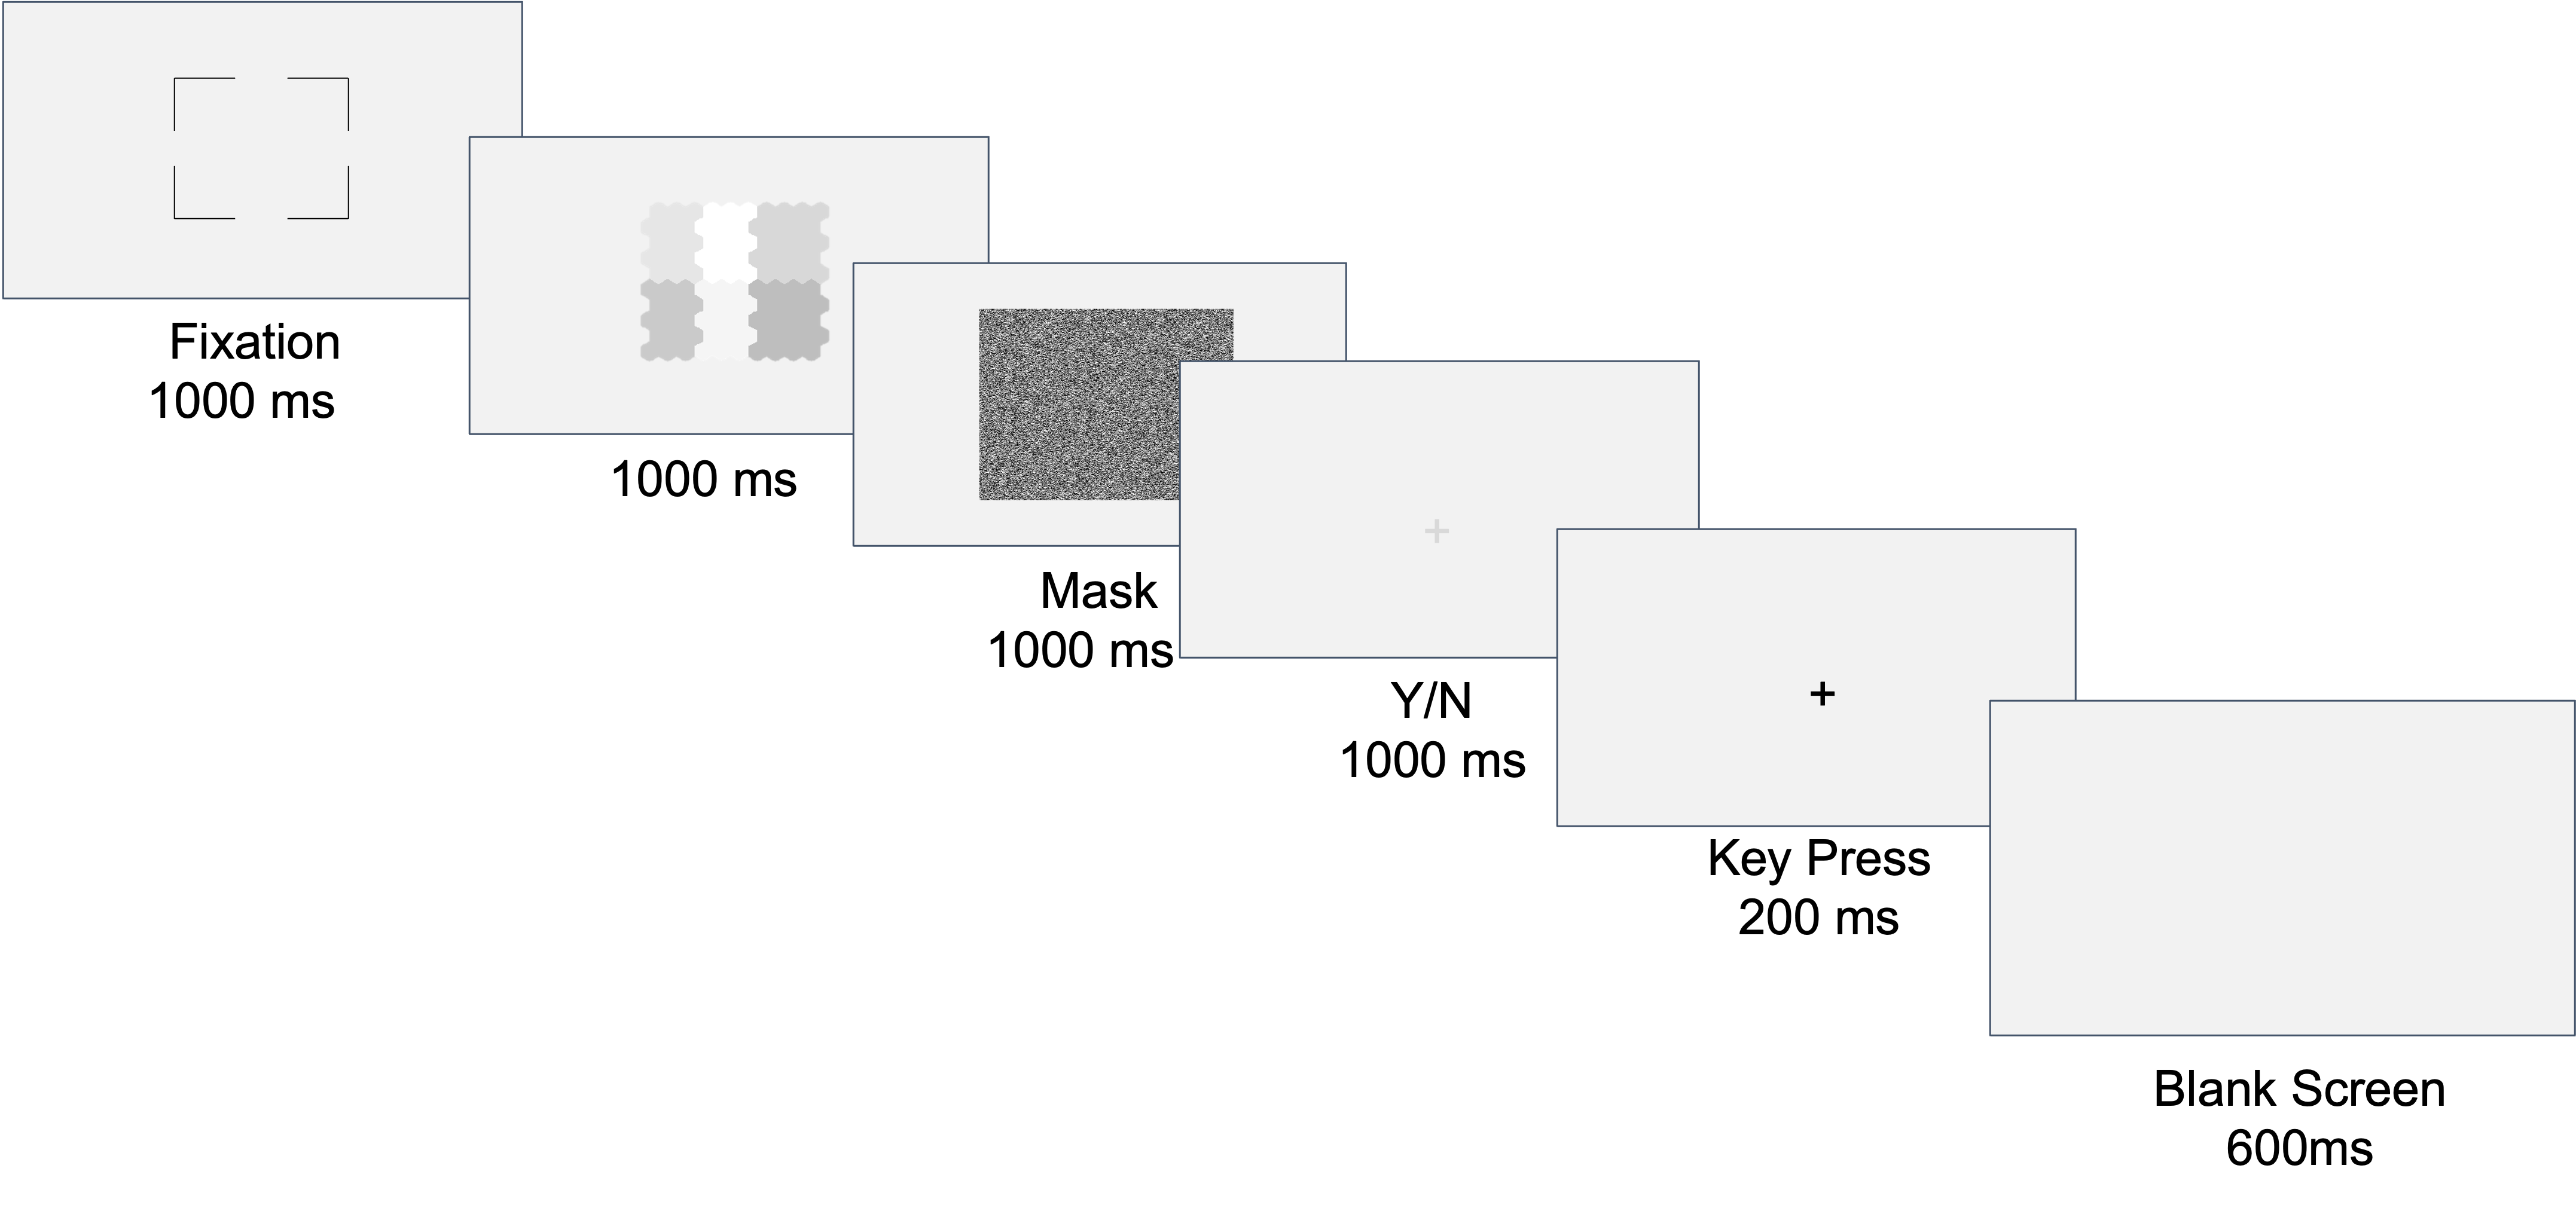
\includegraphics[width=\textwidth]{images/thr_exp_procedure.png}
    \caption{Trial sequence and stimuli in the pre-experiment task. The image contained 6 segments defined by their different intensity values. The borders of the segments remained the same throughout the trials. But the intensity differences between them differed. After the mask, participants had to submit their responses.
    They were instructed to press the "Yes" key (up arrow key) if they saw all 6 segments in the image or the "No" key (down arrow key) if they did not. Their responses were submitted only during the response phase. The duration of the response phase was limited to 1000 ms. After the response was submitted, the fixation cross changed its color to black from gray. Following a brief blank screen, a new trial began.}
    \label{fig:thr_exp_procedure}
\end{figure}


\subsection{Experiment}
The purpose of this task was to investigate whether increased access to computational resources could enhance the detection of image segments resulting from further partitioning. To test this, we conducted an experiment where we manipulated the exposure time of our stimuli. Additionally, we aimed to explore whether image segmentation occurs hierarchically in human visual perception. To do so, we employed normalized min-cut algorithm that segments images hierarchically and presented the resulting segments at various levels of this process. By measuring the accuracy of participants at these levels, we were able to have an estimation regarding human segmentation performance.

\subsubsection{Stimuli}
The experiment was composed of two main stimuli. The first type of stimuli was identical to the one used in the pre-experiment task with one exception. The groups forming the image were generated randomly, and they had different borders at each trial. In order to create these groups, we used the Voronoi diagram (\cite{aurenhammer1991voronoi}). Voronoi diagram is used to partition a plane by assigning each object to the closest pre-determined point. The objects on the plane form regions together, and the number of regions is equal to the number of pre-determined points.

To generate Voronoi regions on our grid $R_k$, we used a 2D coordinate set spanning from 1 to 10, where 1 on the x-axis represents the leftmost hexagon and 1 on the y-axis represents the topmost hexagon. We then placed six points $l_k$ on the grid, which were selected to divide the grid into equal parts. The locations of these points were stored in set $K$. To randomize their location for each trial, we sampled six different values from a standard normal distribution for both coordinates and added them to the original locations.

The Voronoi region $R_k$ for a point $x \in X$ is defined as:

\begin{equation}
R_k = {x \in X | d(x, l_k) \geq d(x, l_j) \text{ for all } j \neq k}
\end{equation}

where $d(x, A)$ is the Euclidean distance between point $x$ and set $A$:

\begin{equation} \label{vor_dist_func}
d(x, A) = \sqrt{(x_1 - A_1)^2 + (x_2 - A_2)^2}
\end{equation}

We used the six points in set $K$ as the reference points $l_k$, i.e., $l_k \in K$, where $K = {(2,3), (5,3), (8,3), (2,7), (5,7), (8,7)}$.


To assign hexagons $x$ to the closest Voronoi region $R_k$, we calculated the Euclidean distance between each hexagon and the points $l_k$, using the distance function $d(x,A)$ (see Equation \ref{vor_dist_func}).

Once hexagons were assigned to their closest Voronoi regions, all hexagons within a region $R_k$ were mapped to the same intensity value from set $I$ that we calculated in the pre-experiment (see Equation \ref{calcInt}). The minimum intensity value for all segments was the same across participants, but the maximum intensity value depended on the participant's contrast sensitivity. To prevent segments with close intensity values from neighboring each other in every trial, we randomized the order of the intensity values in set $I$.  

The second set of stimuli was the segments that formed the image. In order to quantify their order in the hierarchy, and the difficulty to be partitioned, we retrieved these segments using the normalized min-cut algorithm (\cite{RN165}) as it was discussed in section \ref{imageSegmentation}.

Images used in the experiment were generated prior to the experiment and formed a data set consisting of 100000 partitioned images. This data set was used for all participants, and the images were chosen randomly. Only leaf segments, segments that do not require further partitioning, were used in the experiment. This decision was made to avoid any potential confounds that could arise from combining multiple segments, which may require additional cognitive processing and could be perceived as novel segments by the observer.

\subsubsection{Foils}
To compare the performance of participants with the control condition, segments matching the target cut no but which were not part of the tested image were presented. These segments were part of the images which were generated prior to the experiment as those used to generate the images for test conditions. The set of control condition consisted of 50000 partitioned images.

In order to control for the potential effects of border overlap, we used a two-step process. First, we selected an image from our image set and randomly chose one of the two segments that matched the target cut no. Next, we extracted the borders of the target segment and assigned a value of 1 to them, as borders are known to be salient cues (\cite{peterson1994object}). We then computed 2D cross-correlations between the target segment and all segments in the presented image. Finally, we normalized the results by dividing them by the number of border hexagons in the comparison segment, resulting in values between 0 and 1. Cross-correlations were also computed after the target segment is rotated $90 \degree$, $180 \degree$, and $270 \degree$.  Computing cross-correlations helped us to take segments' border similarity in different locations in the image into consideration. 

To account for the limitation of cross-correlation in evaluating the combination of multiple segments, we conducted an additional step by creating a set of border hexagon coordinates. We then computed the number of total overlaps by comparing these coordinates with those of the target foil hexagons. This total overlap number was divided by the total number of hexagons in the target foil to obtain a score. If both this score and all values in the cross-correlation matrix were below 0.4, the target foil was selected. This method provided a more comprehensive evaluation of target foil suitability by taking into account not only individual hexagon similarities but also their combination as a whole. \label{crossCorr}

If any of the segments from the presented image had overlapping borders above the threshold, another image from the pre-generated set was used. This search continued until all the segments from the presented image have overlapping borders with any of the foils less than the threshold. As in the test condition, only the leaf segments were used in the control condition.

\subsubsection{Procedure}
Figure \ref{fig:exp_procedure} illustrates the procedure of a single trial from the experiment. Each trial started with a fixation window which covered the area of the presented stimulus for 1000 ms with the markings at the four corners. It was followed by a grid image. Images were chosen from the data set that we generated prior to the experiment. Their presentation duration varied depending on the exposure time condition. For the short exposure time, images were shown for 200 ms whereas for the long exposure time duration was 1000 ms. The image was followed by a static white noise mask for 1000 ms. Then, participants were presented a segment. In the test condition, one segment resulting from the partitioning of the presented image was shown. This segment could belong to any of the five possible cuts, ranging from the first cut (cut no. 1) to the final cut (cut no. 5). In the control condition, partitioning of a non-shown image was used. If the target segment with the same cut no from that image satisfied the similarity conditions, the segment was presented. Segments were displayed on the screen for 2000 ms. Their location in the image was preserved. However, they were shown with the average intensity value of the image. The response phase started with the response screen containing a white fixation cross which was located at the center of the screen. The participants were required to press the "Up" arrow key to indicate that they saw this segment as a part of the image or the "Down" arrow key to indicate that they did not see the segment. Following their key press, the fixation cross changed its color to black to provide feedback regarding their response is recorded. Participants were required to submit their responses in 1000 ms. A trial ended with a blank screen which lasted for 600 ms.

Exposure time conditions derived from the results of the preliminary experiments we conducted (Supplementary Materials \ref{pilotExp}). In these experiments segments from cut no 2 and cut no 5 were compared across various durations. Results of the pilot experiment showed that while there is no difference between exposure time conditions in cut no 2 condition, performances in cut no 5 differed. Since the performance in the $0.6$ s condition was lower than the chance level (Figure \ref{fig:expTimeComparison}), we took $0.3$ s and $0.9$ s conditions into consideration. Further, since the average fixation duration is 250 ms (\cite{unema2005time}) and we wanted to include 4 fixations in the long exposure time condition, we set the long exposure time to 1 s.

The task instructions were given to the participants before the experiment started (Supplementary Materials \ref{Instructions}). They were displayed on the screen and also delivered verbally by the experimenter. After the instructions, participants received 40 practice trials each with a response phase lasting 20 seconds. During the first 5 to 10 trials, the experimenter remained in the experiment room to provide guidance. After each practice trial, participants received feedback in the form of a screen displaying information on the accuracy of their response, the presented image, and the presented segment. This feedback allowed participants to better understand the task and improve their performance through comparison. The number of test and control trials were randomized.

\begin{figure}
    \centering
    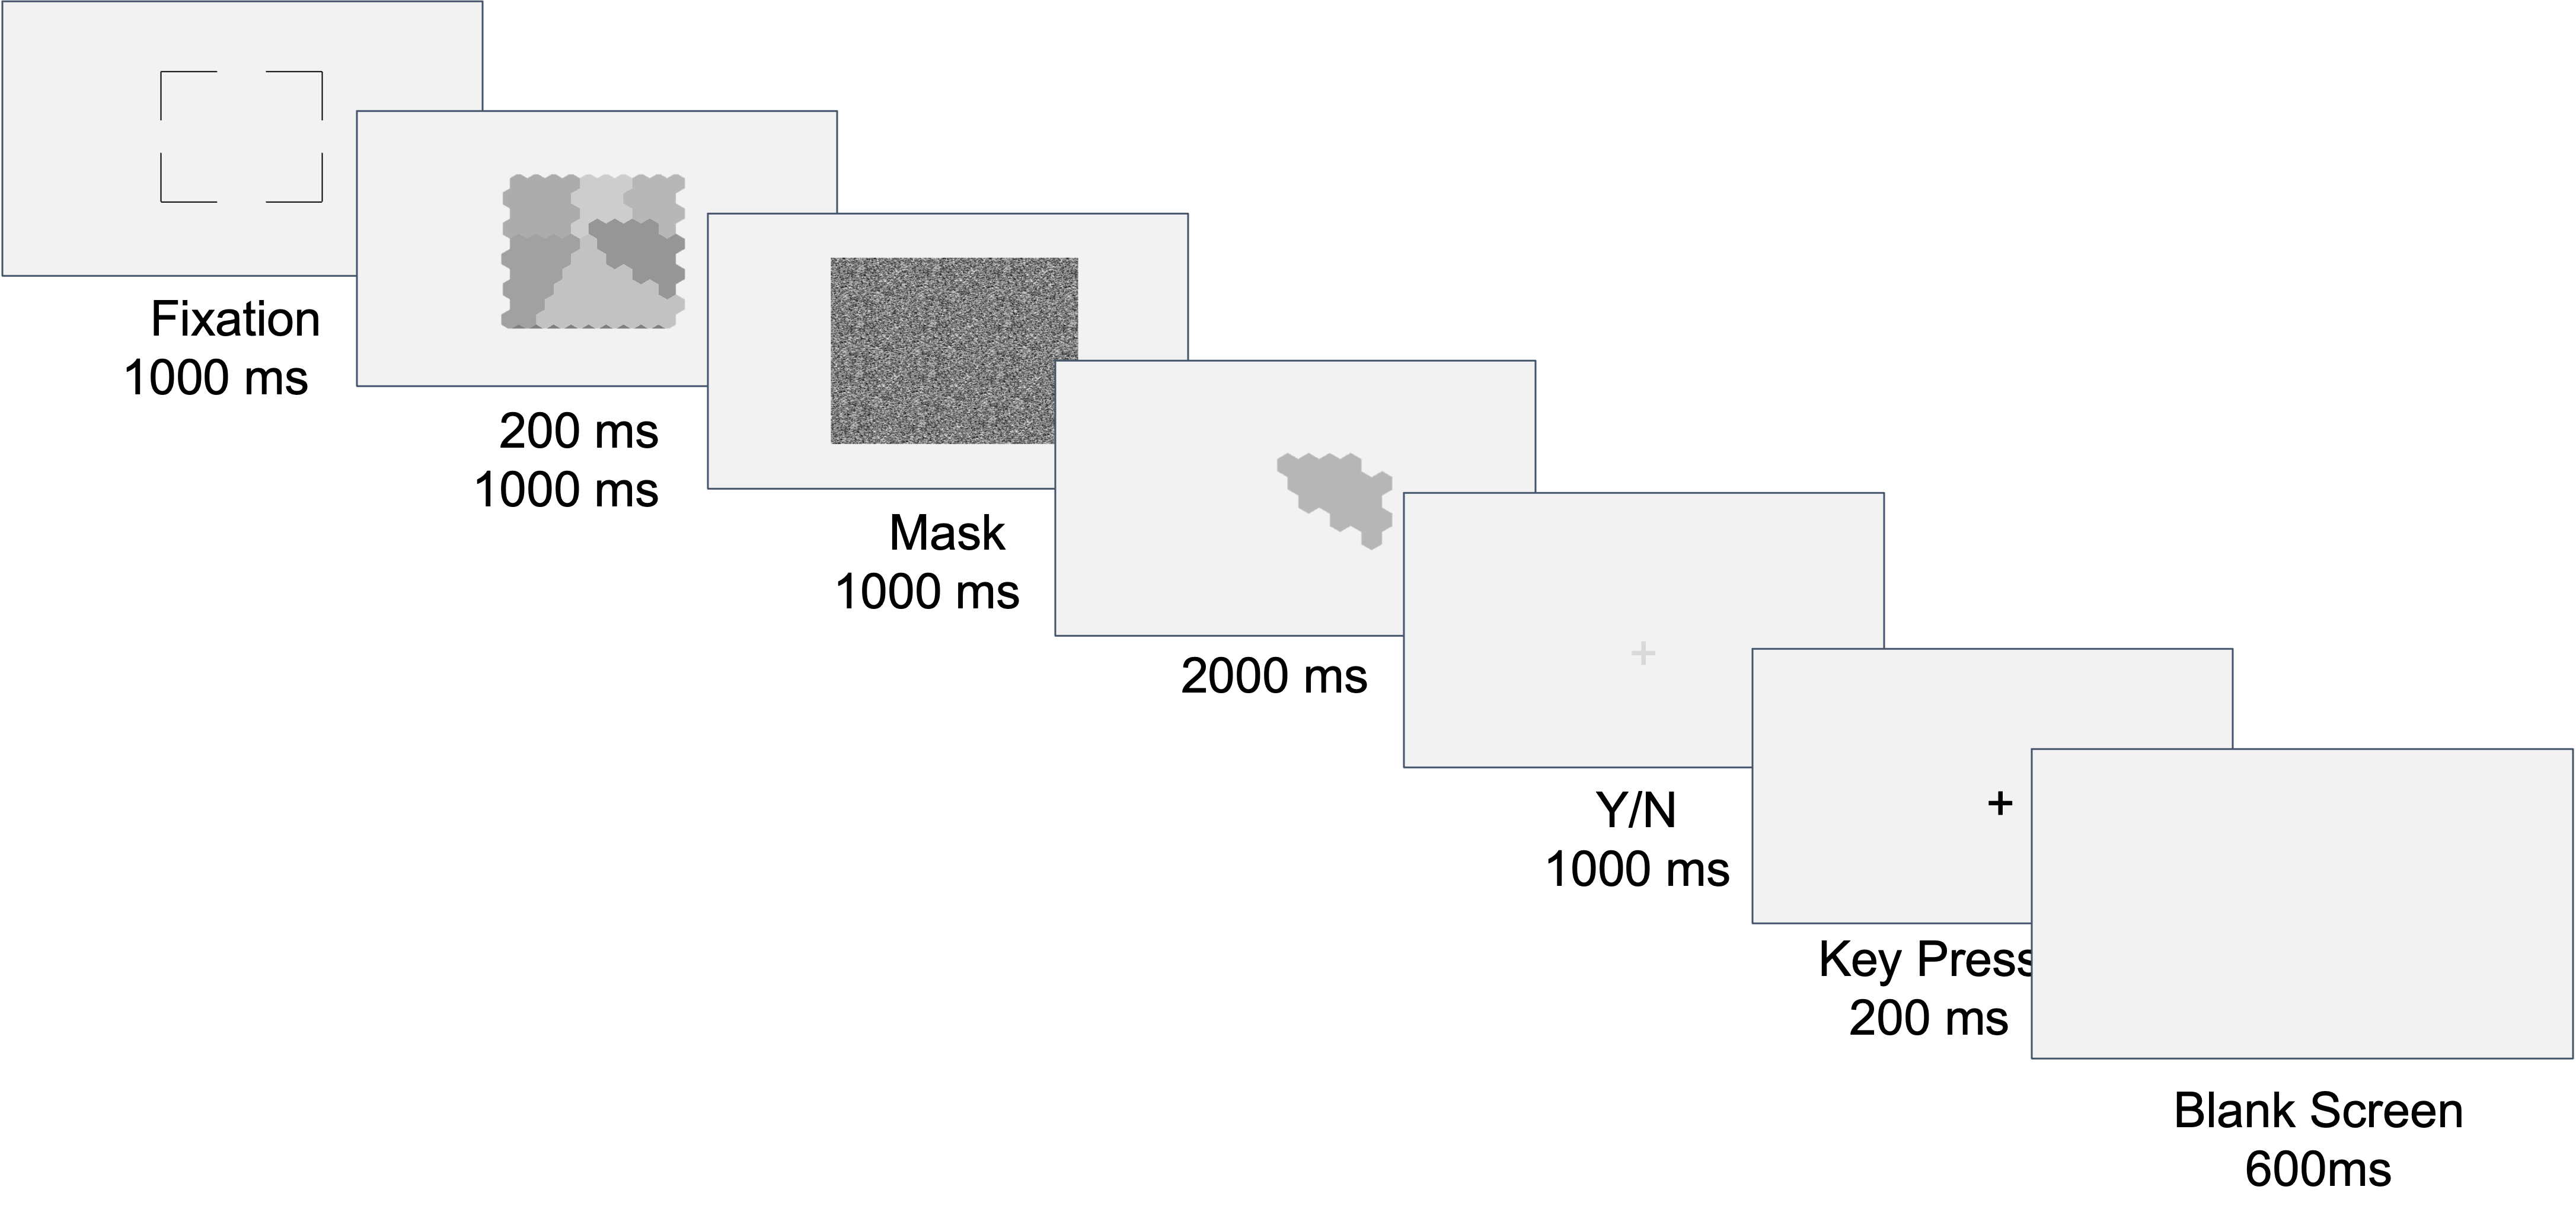
\includegraphics[width=\textwidth]{images/experimentalProcedure.png}
    \caption{Trial sequence and stimuli in the main experiment. It is similar to the procedure used in the pre-experiment with only a few exceptions. In this task, the borders of the segments were dynamic throughout the trials but the same intensity mappings were used. We also manipulated the exposure time. The short exposure time was set to be 200 ms, whereas the long exposure time was 1000 ms. After the mask, either a segment that belonged to the presented image (test trial) or a foil (control trial) was displayed. The duration of this display was 2000 ms. Participants were instructed to press the "Yes" key (up arrow key) if they saw the segment in the image or the "No" key (down arrow key) if they did not. After the response was submitted in the response phase, the fixation cross changed its color to black from gray. Following a brief blank screen, a new trial began.}
    \label{fig:exp_procedure}
\end{figure}


\subsubsection{Design}
The experimental design was 2 (Control/Test) x 2 (Exposure Time) x 5 (Cut No) with Yes/No procedure. There were 100 trials for each condition and participants were tested in 25 blocks of 80 trials each. At the end of each block, the participants were given feedback on their accuracy. They were also allowed to take a break between blocks. The entire experiment lasted around four and a half hours.


\section{Results}
\subsection{Fitting Data Using Logistic Regression}
In this study, we aimed to investigate the effects of exposure time, cut no, and other factors on test and control trials. To achieve this, we employed a series of generalized linear models (GLM), with different regressors for each trial type due to potential differences in the underlying factors (\ref{fig:regressors}).


\begin{figure}[!ht]
    \centering
    
    \begin{subfigure}[t]{0.35\textwidth}           
        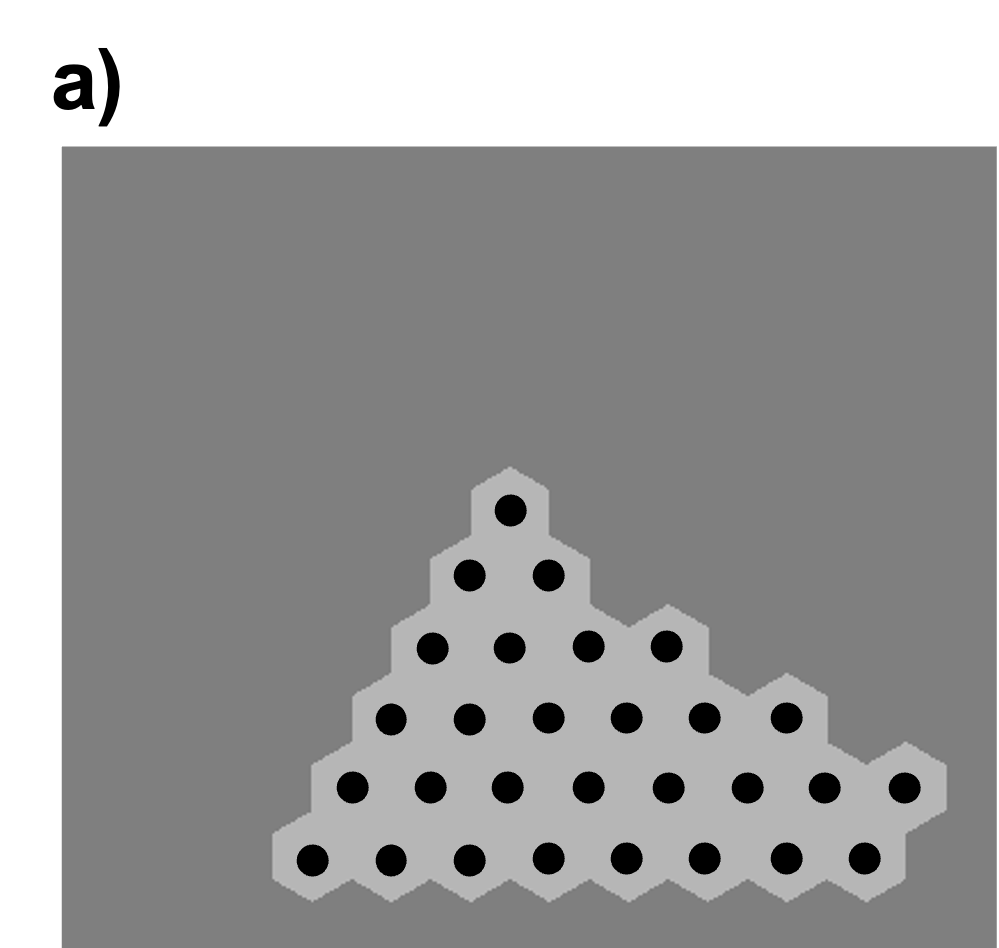
\includegraphics[width = \linewidth]{plots/pred_segSize.png}
        \caption{Computing the segment size. }
        \label{fig:pred_segSize}    
    \end{subfigure}
    \hspace{0.05\textwidth}
    \begin{subfigure}[t]{0.35\textwidth}           
        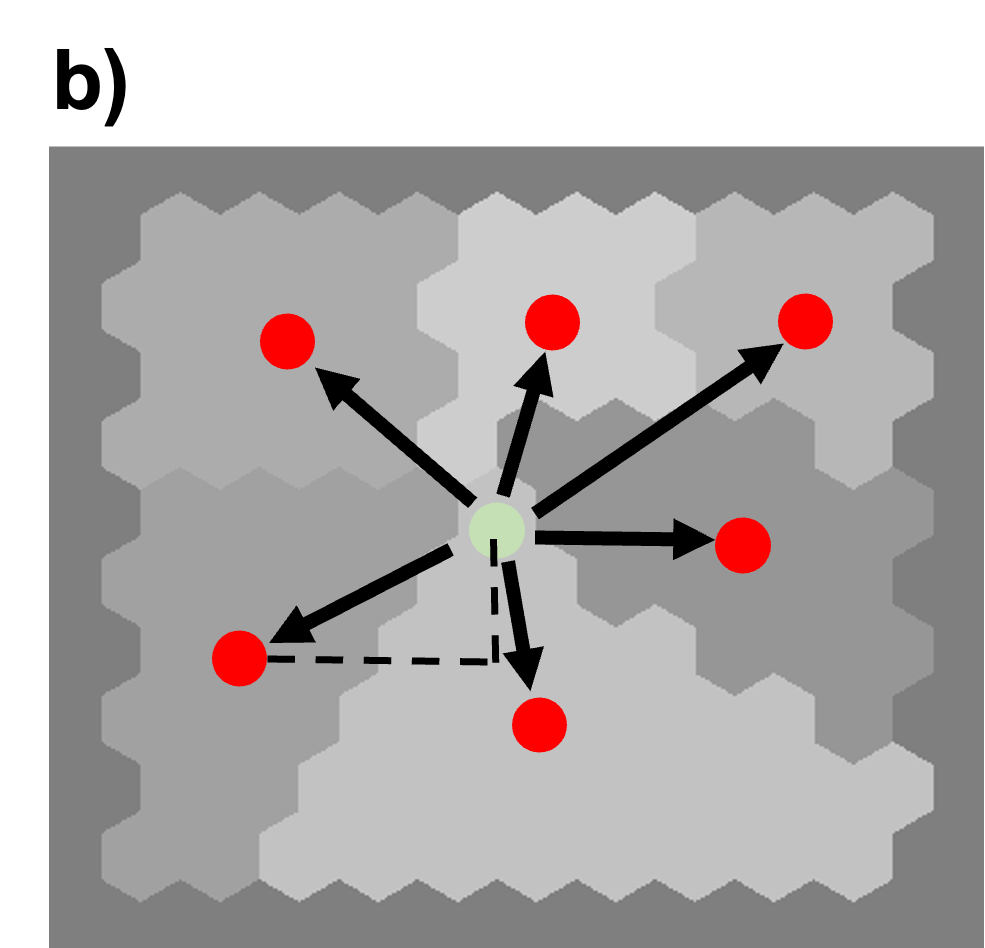
\includegraphics[width = \linewidth]{plots/pred_segDist.png}
        \caption{Computing the segment distance to the center of the image. }
        \label{fig:pred_segDist}    
    \end{subfigure}
        
        
    \begin{subfigure}{\textwidth}          
        \centering
        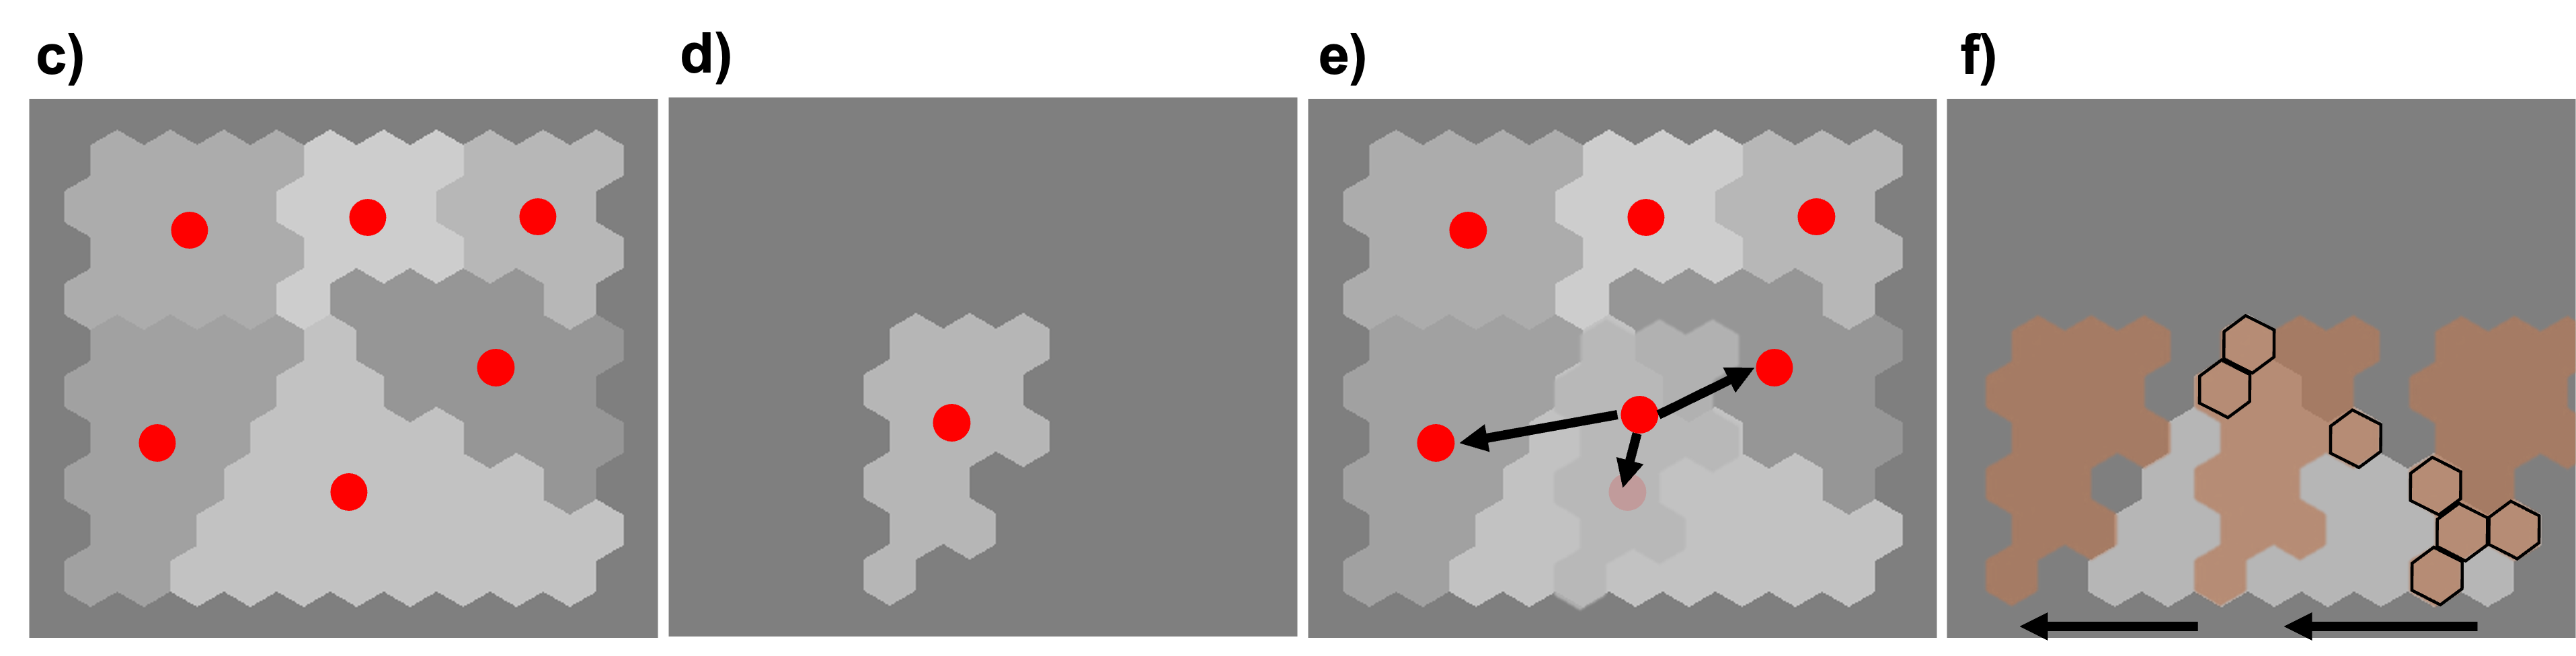
\includegraphics[width = \linewidth]{plots/pred_control.png}
        \caption*{(c,d,e,f,g) Computing the highest similarity and closest segment's cut no.}
        \label{fig:pred_control}    
    \end{subfigure}    
    \label{fig:regressors}
    \caption{Computation of some of the predictors used in the regression models. \textbf{a.} Each black dot represents the centers of the hexagons. The number of hexagons is used to compute segment size. \textbf{b.} Each red dot represents the centers of the segments forming the image. The center of the image is highlighted with a green dot. Euclidian distances between the red dot and green dot give us the segment distance to the center. \textbf{c.,d.,e.,f.,g.} Showing the process of computing highest similarity and closest segment cut no. \textbf{c.} shows the center of the segments in the presented image. \textbf{d.} shows the center of the presented foil. \textbf{e.} shows the process of finding the closest segment in the image. We then used the cut no of the image segment with the shortest distance as the closest segment predictor. \textbf{f.} shows three steps of cross-correlation computations. Outlined hexagons are the border overlaps between the foil and the closest segment in the image.}
\end{figure}

\subsubsection{Separate Generalized Linear Models for Participants}
We first fitted separate models for participants due to subjective contrast sensitivities. For the test trials, we included predictors such as exposure time (a categorical variable with two conditions: short and long), cut no (a continuous variable derived from the order of partitioning and ranging between 1 to 5, see \ref{cutNo}), segment size (the total number of hexagons in the presented segment), segment distance (the Euclidean distance of the segment's center to the center of the image), intensity difference (the difference between the average image intensity and the target segment's intensity in the presented image), intensity order (order of segment intensities ranging from 1 to 5) and cumulative effort. The cumulative effort was computed by summing up the $Ncut$ values up to the previous cut. Since further partitioning was not possible for the leaf segments, 0 was assigned as $Ncut$ value. We standardized all predictors except cut no and exposure time to fall within the range of 0 and 1.


For the control trials, we replaced cut no with the closest segment's cut no as a predictor. We computed it by finding the center of each segment in the presented image and computing their distances to the center of the target segment. Among those distances, the image segment with the closest distance to the presented control segment was chosen. Later, this image segment's cut no was used as the closest segment predictor. Another predictor used in testing control trials is the highest similarity. Since previous research showed that contours and orientation contrasts are playing important roles in object recognition and texture segmentation (\cite{peterson1994object}, \cite{nothdurft1991texture}), we used border similarity as a similarity measure. In order to compute this predictor, cross-correlation between the foil and the closest segment in the presented image was computed. Then the highest value in the resulting matrix was assigned. This value was also normalized before being used in the model. Other predictors from the test models were kept the same and used for control condition models.

The response variable for both test and control trial models was the accuracy of participants, and it was modeled using the log-link function. Since participants were tested with their subjective contrast sensitivities, separate regression models were fit for each. Individual performances and reconstructed model performances can be seen in Figure \ref{fig:behav_test} and \ref{fig:behav_control}.

\begin{figure}    
    \vspace{-1.3cm}
    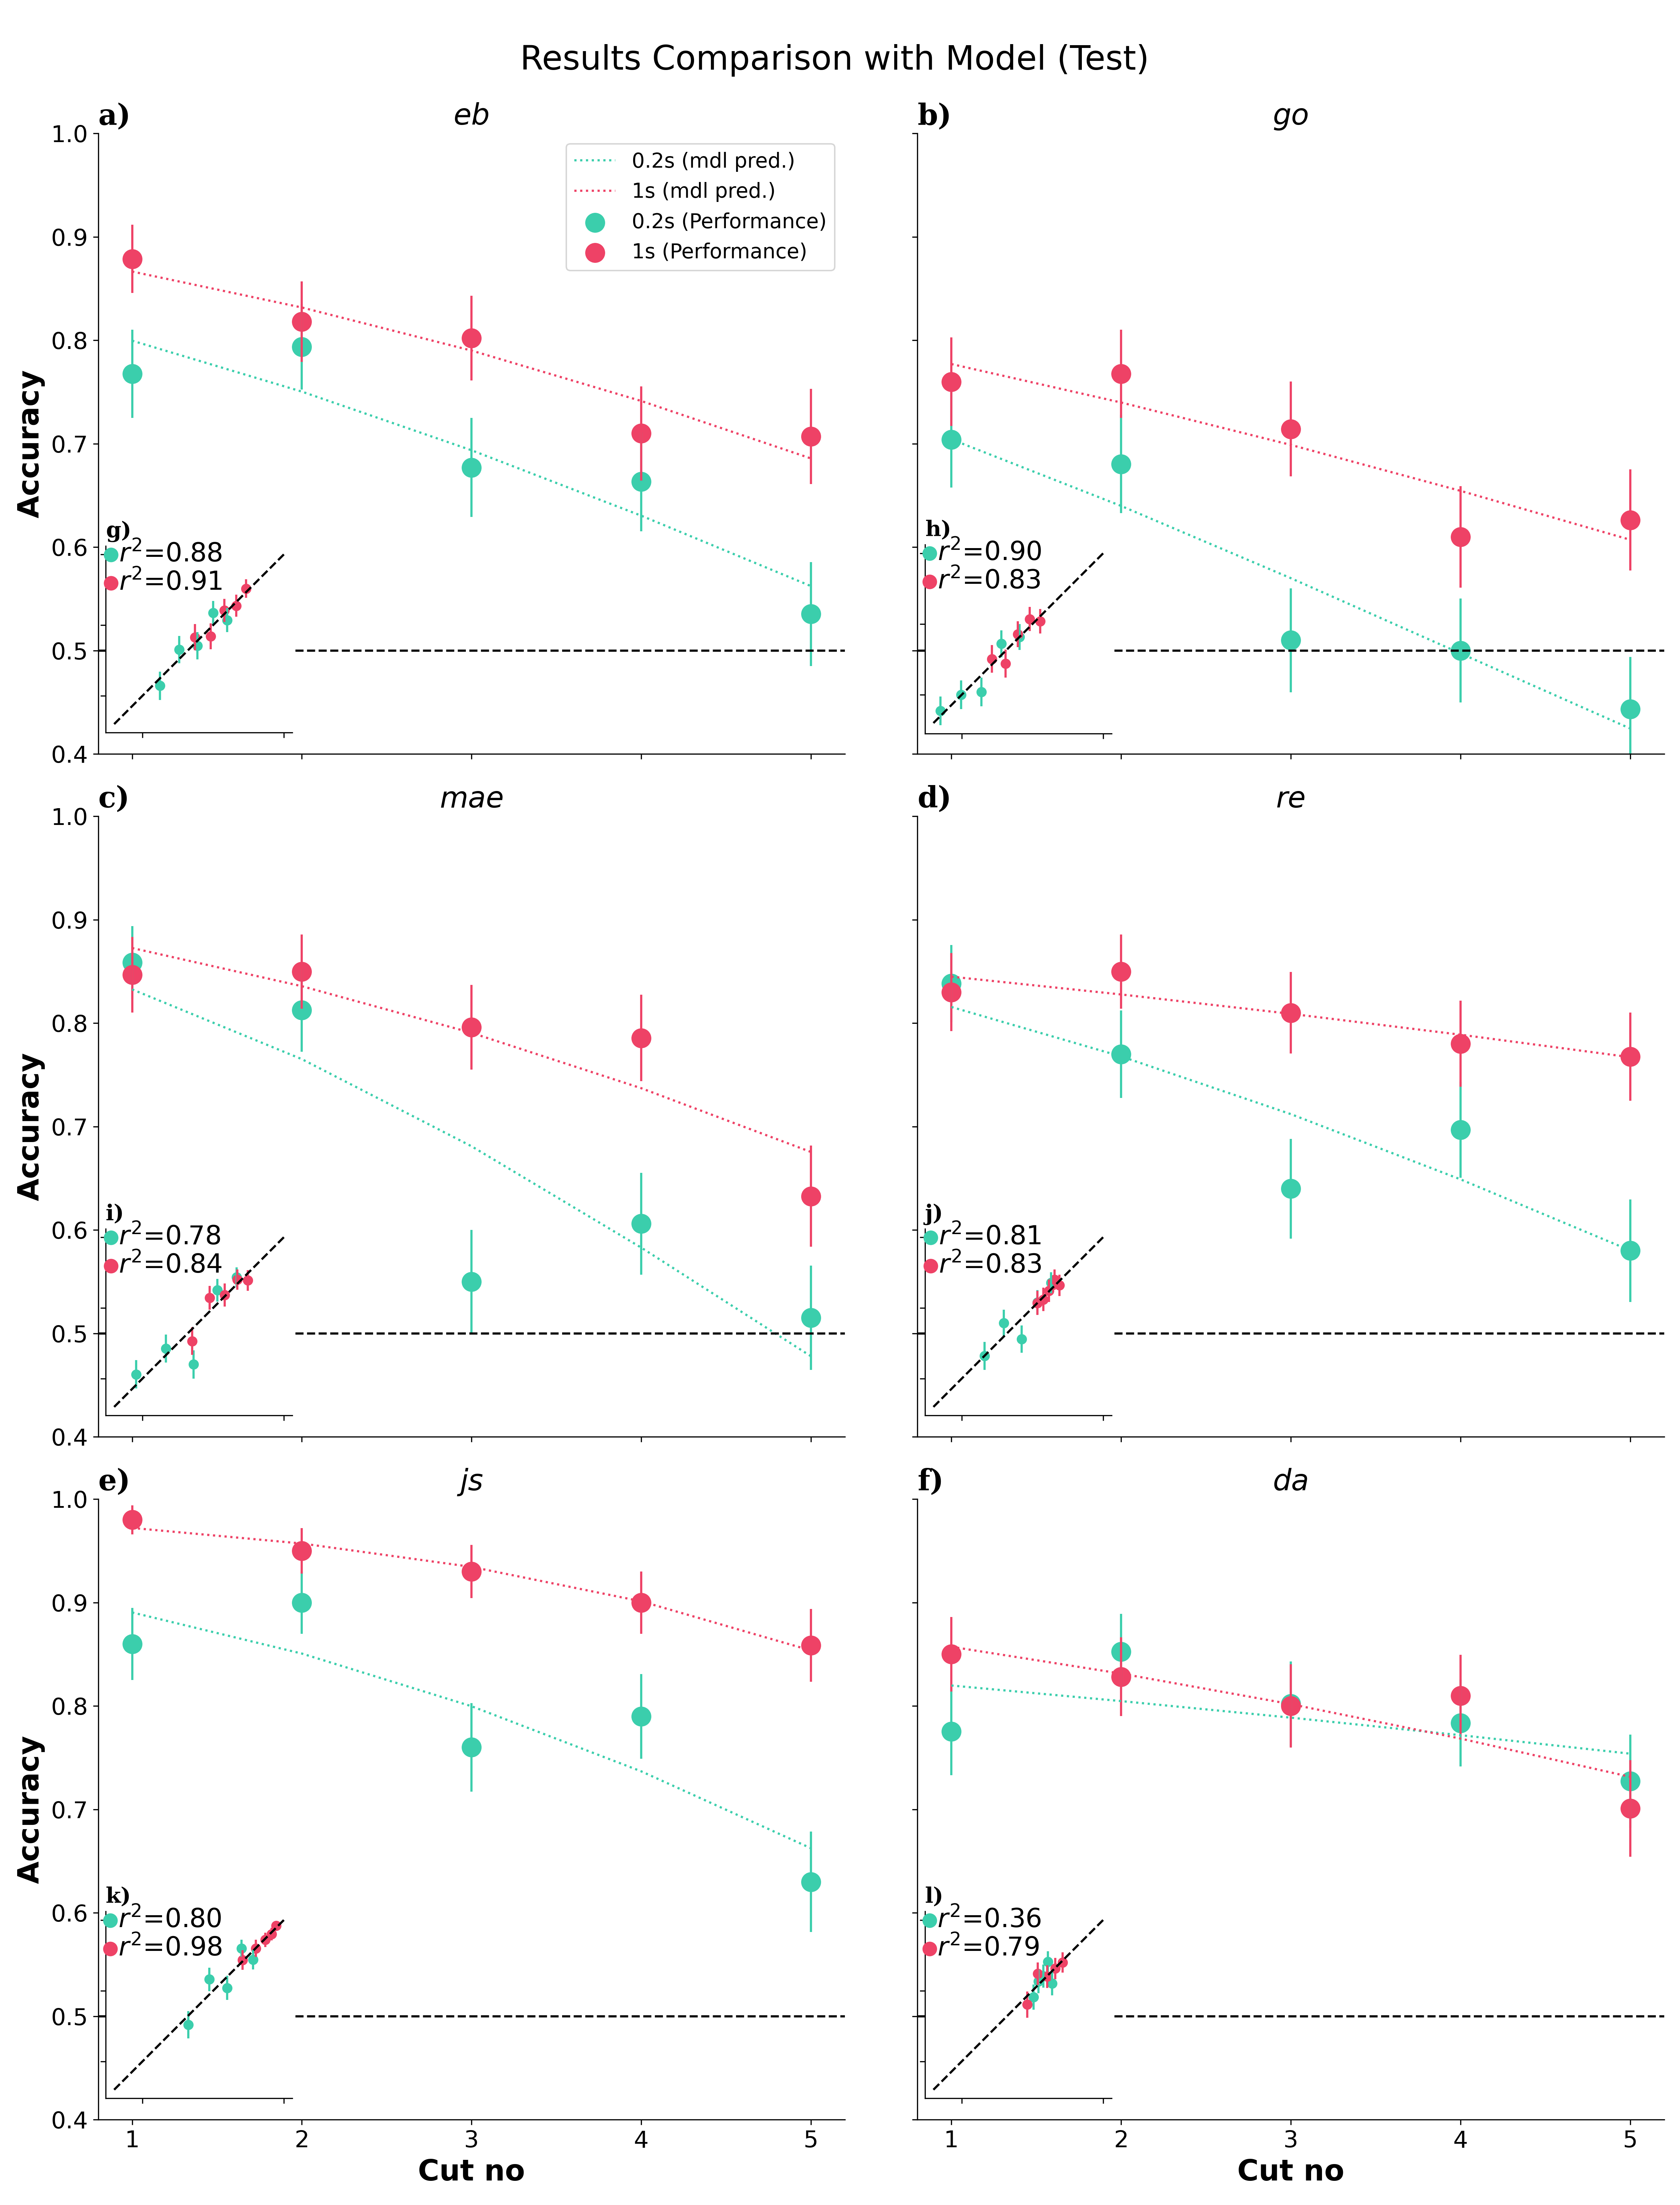
\includegraphics[width=\textwidth]{plots/test_all.png}    
    \caption{\textbf{a, b, c, d, e, f, g.} Behavioral results of participants for test trials. Accuracies for short (blue) and long (red) exposure time conditions across cut no can be seen with the dots. Error bars represent the standard error of the means. Dotted lines are reconstructions of results using generalized linear models. The models used for reconstructions have the following formula: $\it{glm(correct \sim Cut No * Exposure Time)}$ \textbf{g, h, i, j, k, l.}, show how good the model predictions fit actual performances of individual participants. $r^2$ scores are written in the legend for convenient comparisons. }
    \label{fig:behav_test}
\end{figure}

\begin{figure}    
    \vspace{-1cm}
    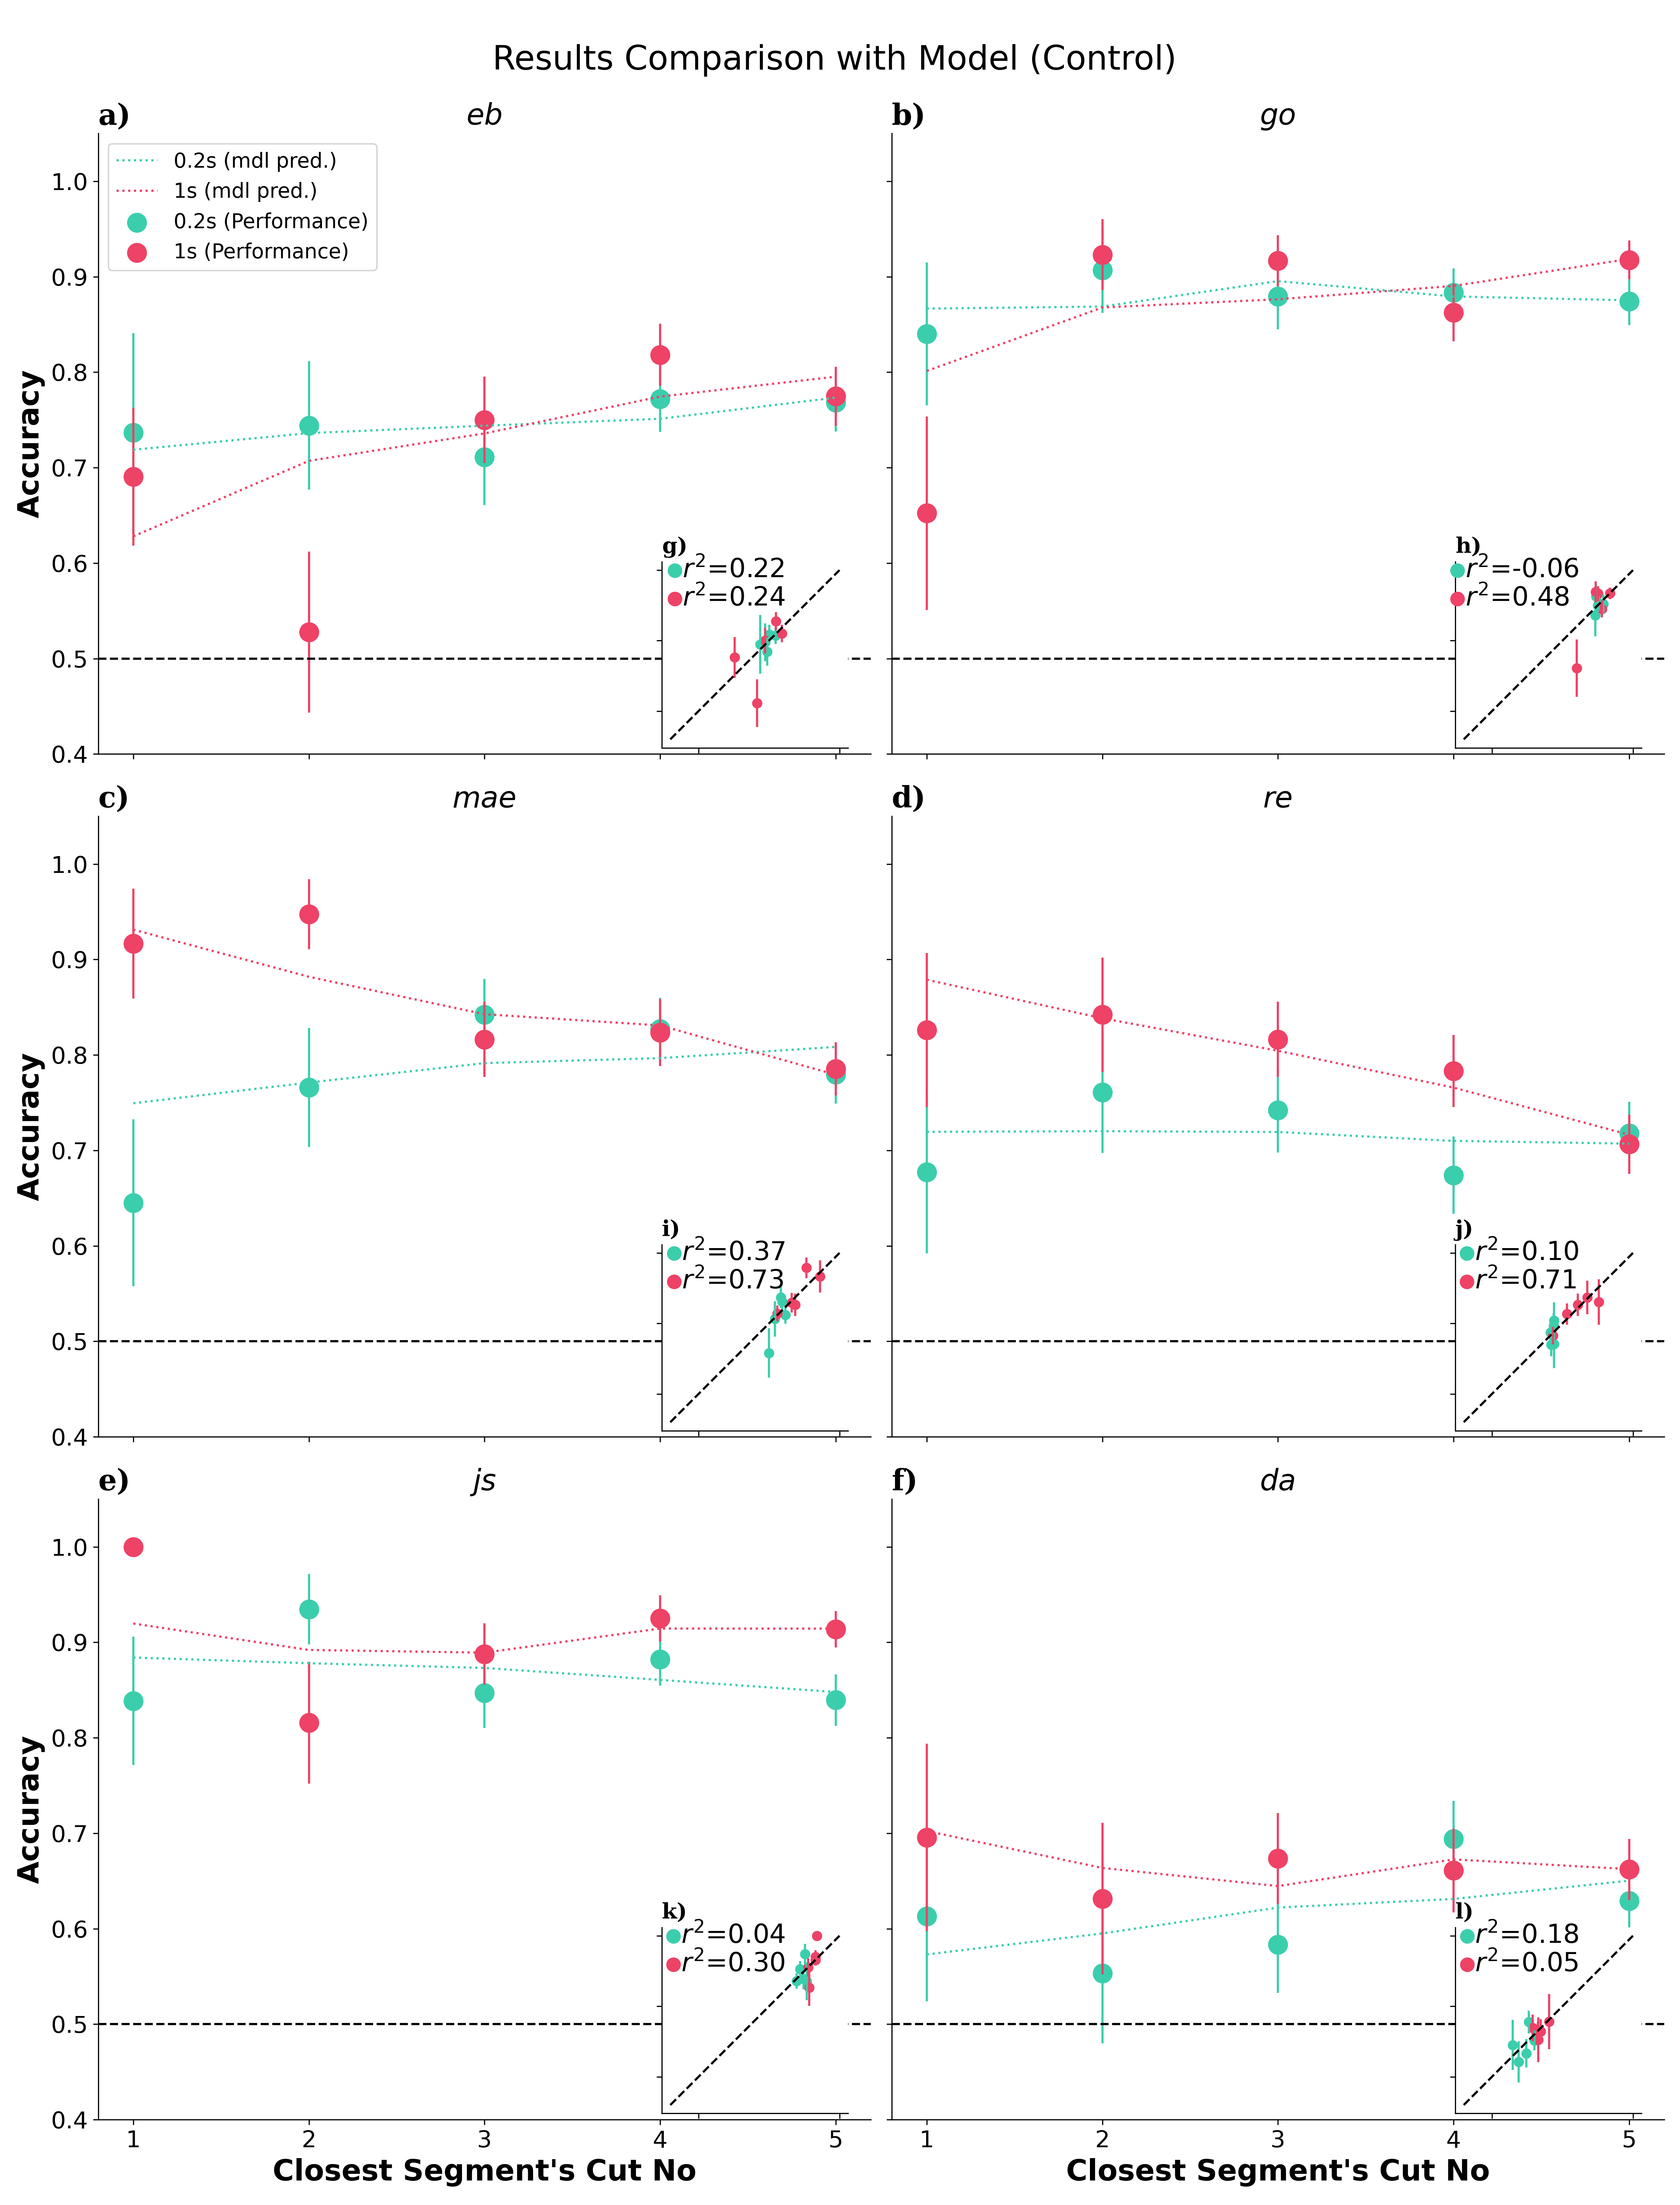
\includegraphics[width=\textwidth]{plots/cntrl_all.png}    
    \caption{\textbf{a, b, c, d, e, f, g.} Behavioral results of participants for the control condition. Accuracies for short (blue) and long (red) exposure time conditions across the closest segment's cut no can be seen with the dots. Error bars represent the standard error of the means. Dotted lines are reconstructions of results using generalized linear models. The models used for reconstructions have the following formula: $\it{glm(correct \sim Closest Cut No * Exposure Time)}$ \textbf{g, h, i, j, k, l.}, show how good the model predictions fit actual performances of individual participants. $r^2$ scores are written in the legend for convenient comparisons. }
    \label{fig:behav_control}
\end{figure}

\begin{figure}[!ht]
    \centering
    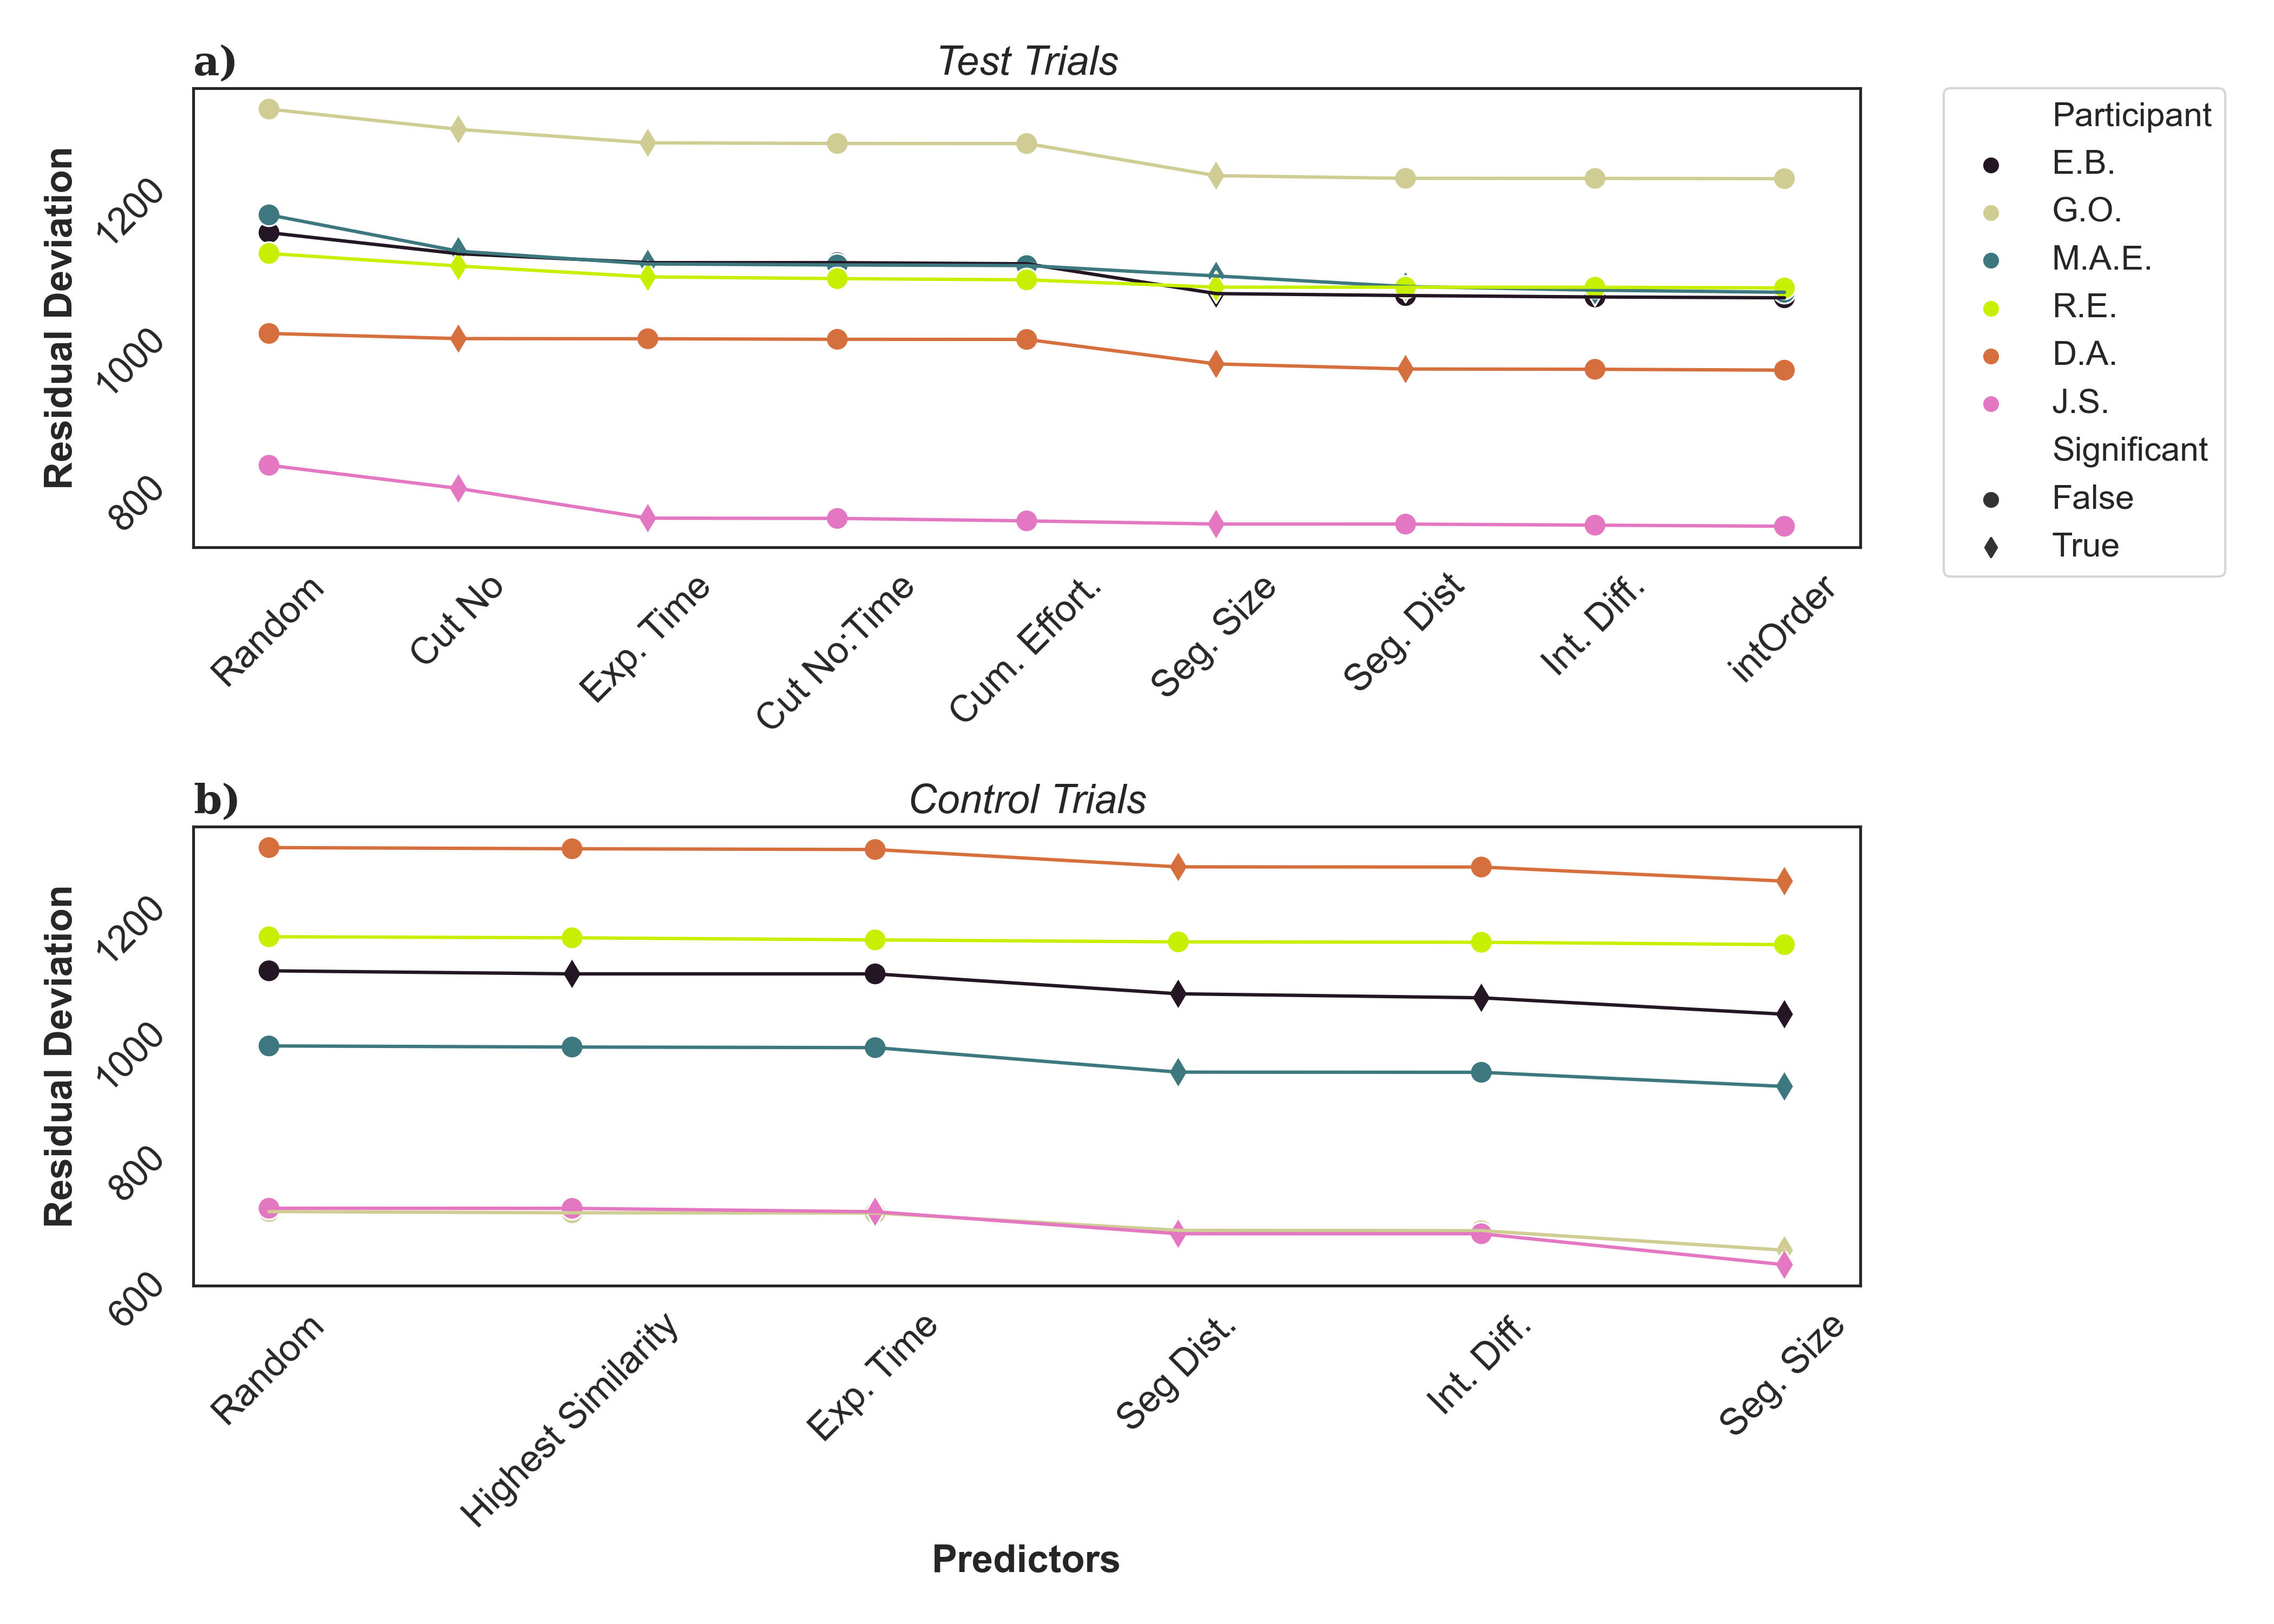
\includegraphics[width=\textwidth]{plots/anova_combined.png}
    \caption{Model comparison results with the increasing number of predictors using $\chi^2$ test. We examined how residual deviations change significantly with the addition of new predictors in each model. \textbf{a.} shows the residual deviations for test trials. \textbf{b.} shows the residual deviations for control trials.}
    \label{fig:anova_cumulative}
\end{figure}


Model comparison was conducted using Chi-square tests in R (\cite{R}). Models were compared with each other after a new variable was added to the model to check if the residual deviance significantly differed. 

\setlength{\tabcolsep}{3pt}
\renewcommand{\arraystretch}{0.6} % Default value: 1
\begin{table}[!h]
    \hspace*{-1.6cm} 
    \caption{\textbf{$p$ Values for test trials after $\chi^2$ tests for residual deviations.} }
    \label{table:test_p_vals}    
    \resizebox{\textwidth}{!}
    {
    \begin{tabular}{c|c c c c c c c c}
    \hline
    Id &  Cum. Eff. & Cut No &  Cut No:Time & Exp. Time &  Int. Diff. &  Seg. Dist & Seg. Size &  Int. Order \\    
    \hline
    D.A.  &         0.698 &   \textbf{0.008} &        0.381 &      0.690 &       0.554 &      \textbf{0.009} &      \textbf{$<$.001} &     0.276 \\
    E.B.  &         0.215 &   \textbf{$<$.001} &        0.919 &      \textbf{0.001} &       0.166 &      0.105 &      \textbf{$<$.001} &     0.298 \\
    G.O.  &         0.769 &   \textbf{$<$.001} &        0.356 &      \textbf{$<$.001} &       0.755 &      0.059 &      \textbf{$<$.001} &     0.570 \\
    J.S.  &         0.070 &   \textbf{$<$.001} &        0.555 &      \textbf{$<$.001}&       0.228 &      0.835 &      \textbf{0.039} &     0.230 \\
    M.A.E &         0.365 &   \textbf{$<$.001} &        0.250 &      \textbf{$<$.001} &       \textbf{0.028} &      \textbf{$<$.001} &      \textbf{$<$.001} &     0.091 \\
    R.E.  &         0.202 &   \textbf{$<$.001} &        0.129 &      \textbf{$<$.001} &       0.857 &      0.743 &      \textbf{0.002} &     0.349 \\
    \hline
    \end{tabular}} \\   
    \captionsetup{labelformat=empty}
    \caption*{\textit{Note:} Results show p values from model comparisons after adding predictors cumulative effort, cut no, exposure time, their interaction, intensity difference, segment distance, segment size, and intensity order after each other. $p$ values smaller than $.05$ were highlighted with bold.}
\end{table}


Model comparisons with the increasing number of predictors for test condition showed that cut no (all $p$ $< .01$) and segment size (all $p$ $< .04$) are significant factors for all participants (Figure \ref{fig:anova_cumulative}). We also observed that except for participant \textbf{D.A}., all participant performances were affected significantly by exposure time (all $p$ $ =< 0.01$). Lastly, segment distance was found to be significant for two participants (\textbf{M.A.E., D.A.}) (all $p$ $<.01$). $p$ values for predictors and participants can be observed in Table  \ref{table:test_p_vals}. $\chi^{2}$ test statistics for all predictors and participants can be seen in Supplementary Materials \ref{participantANOVAs}.



\setlength{\tabcolsep}{3pt}
\begin{table}
    \centering    
    \caption{\textbf{$p$ Values for control trials after $\chi^2$ tests for residual deviations.} }
    \label{table:cntrl_p_vals}
    \begin{tabular}{{c|c c c c c }}
    \hline
    Id &  Exp. Time &  Highest Similarity &  Int. Diff. &  Seg Dist. &  Seg. Size  \\
    \hline
    D.A.  &      0.275 &               0.172 &       0.620 &      \textbf{$<$.001} &      \textbf{$<$.001} \\
    E.B  &      0.935 &               \textbf{0.027} &       \textbf{0.012} &      \textbf{$<$.001} &      \textbf{$<$.001} \\
    G.O.  &      0.574 &               0.164 &       0.450 &      \textbf{$<$.001} &      \textbf{$<$.001} \\
    J.S.  &      \textbf{0.021} &               0.666 &       0.904 &      \textbf{$<$.001} &      \textbf{$<$.001} \\
    M.A.E. &      0.338 &               0.182 &       0.633 &      \textbf{$<$.001} &      \textbf{$<$.001} \\
    R.E.  &      0.068 &               0.197 &       0.438 &      0.075 &      0.052 \\
    \hline
    \end{tabular}
    \captionsetup{labelformat=empty}
    \caption*{\textit{Note:} Results show p values from model comparisons after adding predictors Exposure Time, Highest Similarity, Intensity Difference, Segment Distance, and Segment Size significantly decreased the residual deviations. $p$ values smaller than $.05$ were highlighted with bold.}
\end{table}

\begin{figure}[!hb]
    \centering
    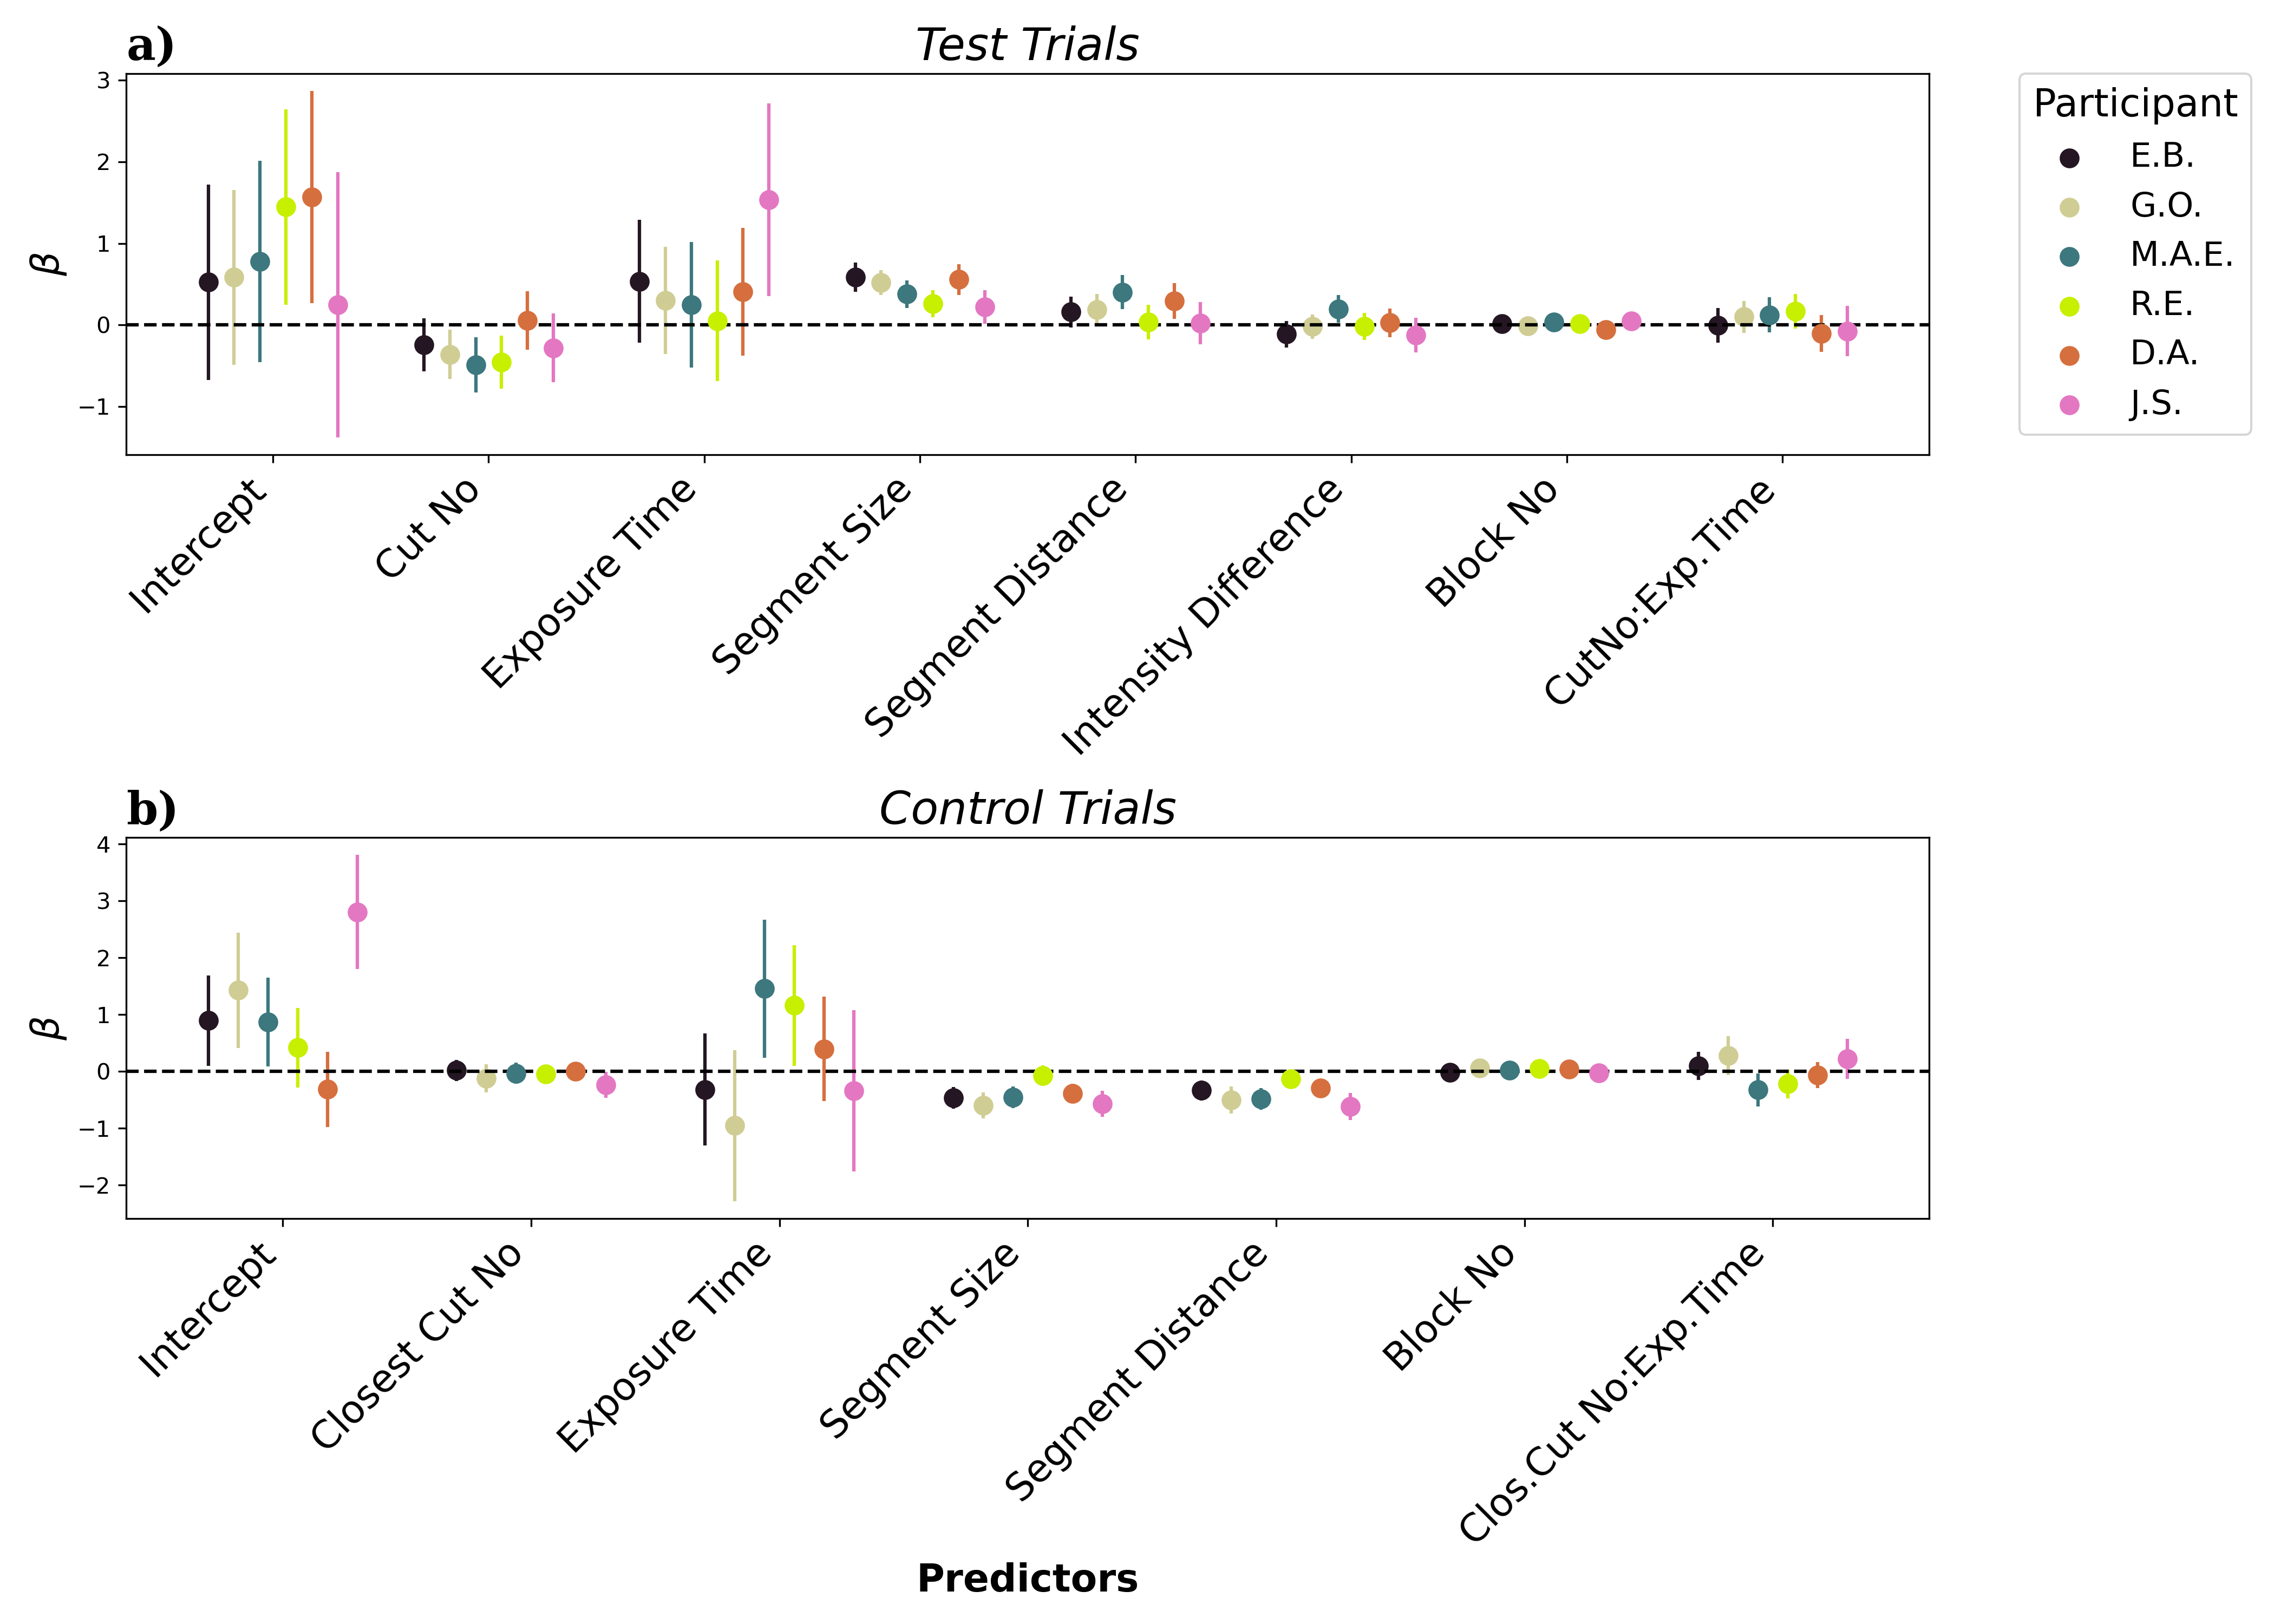
\includegraphics[width=\textwidth]{plots/coefficients_combined.png}
    \hspace{-1cm}
    \caption{Generalized linear models (GLM) when all the predictors are added. Plots show $\beta$ coefficients for all the participants with predictors on the x-axis. \textbf{a.} Results with test trials fit the model. \textbf{b.} Results with only control trials fit the model.}
    \label{fig:glm_coeffs}
\end{figure}


Model comparisons with the increasing number of predictors for the control condition showed that segment distance and segment size are significant factors for all participants except \textbf{R.E.} (all $p$ $< 0.01$) (Figure \ref{fig:anova_cumulative}). We also observed that exposure time is significant for \textbf{J.S}. ($p = 0.02$). The highest similarity ($p = 0.03$) and intensity difference were also found to be significant for \textbf{E.B.} ($p = 0.01$). $p$ values for predictors and participants can be observed in Table \ref{table:cntrl_p_vals}. $\chi^{2}$ test statistics for all predictors and participants can be seen in Supplementary Materials \ref{participantANOVAs}.


For the test trials, when all the predictors were included in a single GLM model for different participants, we observed that the effect of cut no disappears for participants \textbf{D.A.}, \textbf{J.S.}, and \textbf{E.B.} (Figure \ref{fig:glm_coeffs}). This also applies to exposure time and except for \textbf{J.S.}, the effect loses its significance. On the other hand, the effect of segment size and segment distance remains the same as in $\chi^2$ comparisons.

Likewise, when all the predictors are combined in a GLM model to test the control condition, the effect of segment size and distance remains significant except for participant \textbf{R.E.} (Figure \ref{fig:glm_coeffs}). Different from than test model, we also observe different participants (\textbf{R.E.} and \textbf{M.A.E.}) performed better when the exposure time is longer. 

\subsubsection{Mixed-Effects Regression Models}
In addition to constructing separate models for each participant, we estimated a mixed-effects regression model that combined all participant data to analyze the relationship between the dependent variable of accuracy and various independent variables. We used a log-link function in the model. We constructed separate models for test and control trials.

For the test trials, we included a participant-specific effect on cut no in the model as a random effect. In addition, we used cut no, exposure time, their interaction, segment size, segment distance to the center of the image, and intensity difference as fixed predictors. Since intensity difference and order were highly correlated, we did not use intensity order in this analysis (Supplementary Materials \ref{multicol}).

Analysis showed negative effect of cut no ($\beta = -.35, z = -.79, SE = .06, p < .001$). Exposure time, on the other hand, showed a positive effect on accuracy ($\beta = .41, z = 2.85, SE = .14, p = .004$). Additionally, segment size ($\beta = .36, z = 11.34, SE = .32,  p < .001$) and segment distance ($\beta = .19, z = 5.24, SE = .035, p < .001$) were found to be significant. Intensity difference ($\beta = .005, z = .16, SE = .029, p = .88$) and interaction of exposure time and cut no ($\beta = .059, z = 1.46, SE = .04, p = .14$) did not show significant effect.

\begin{figure}[!hb]
    \hspace*{-1.2cm}
    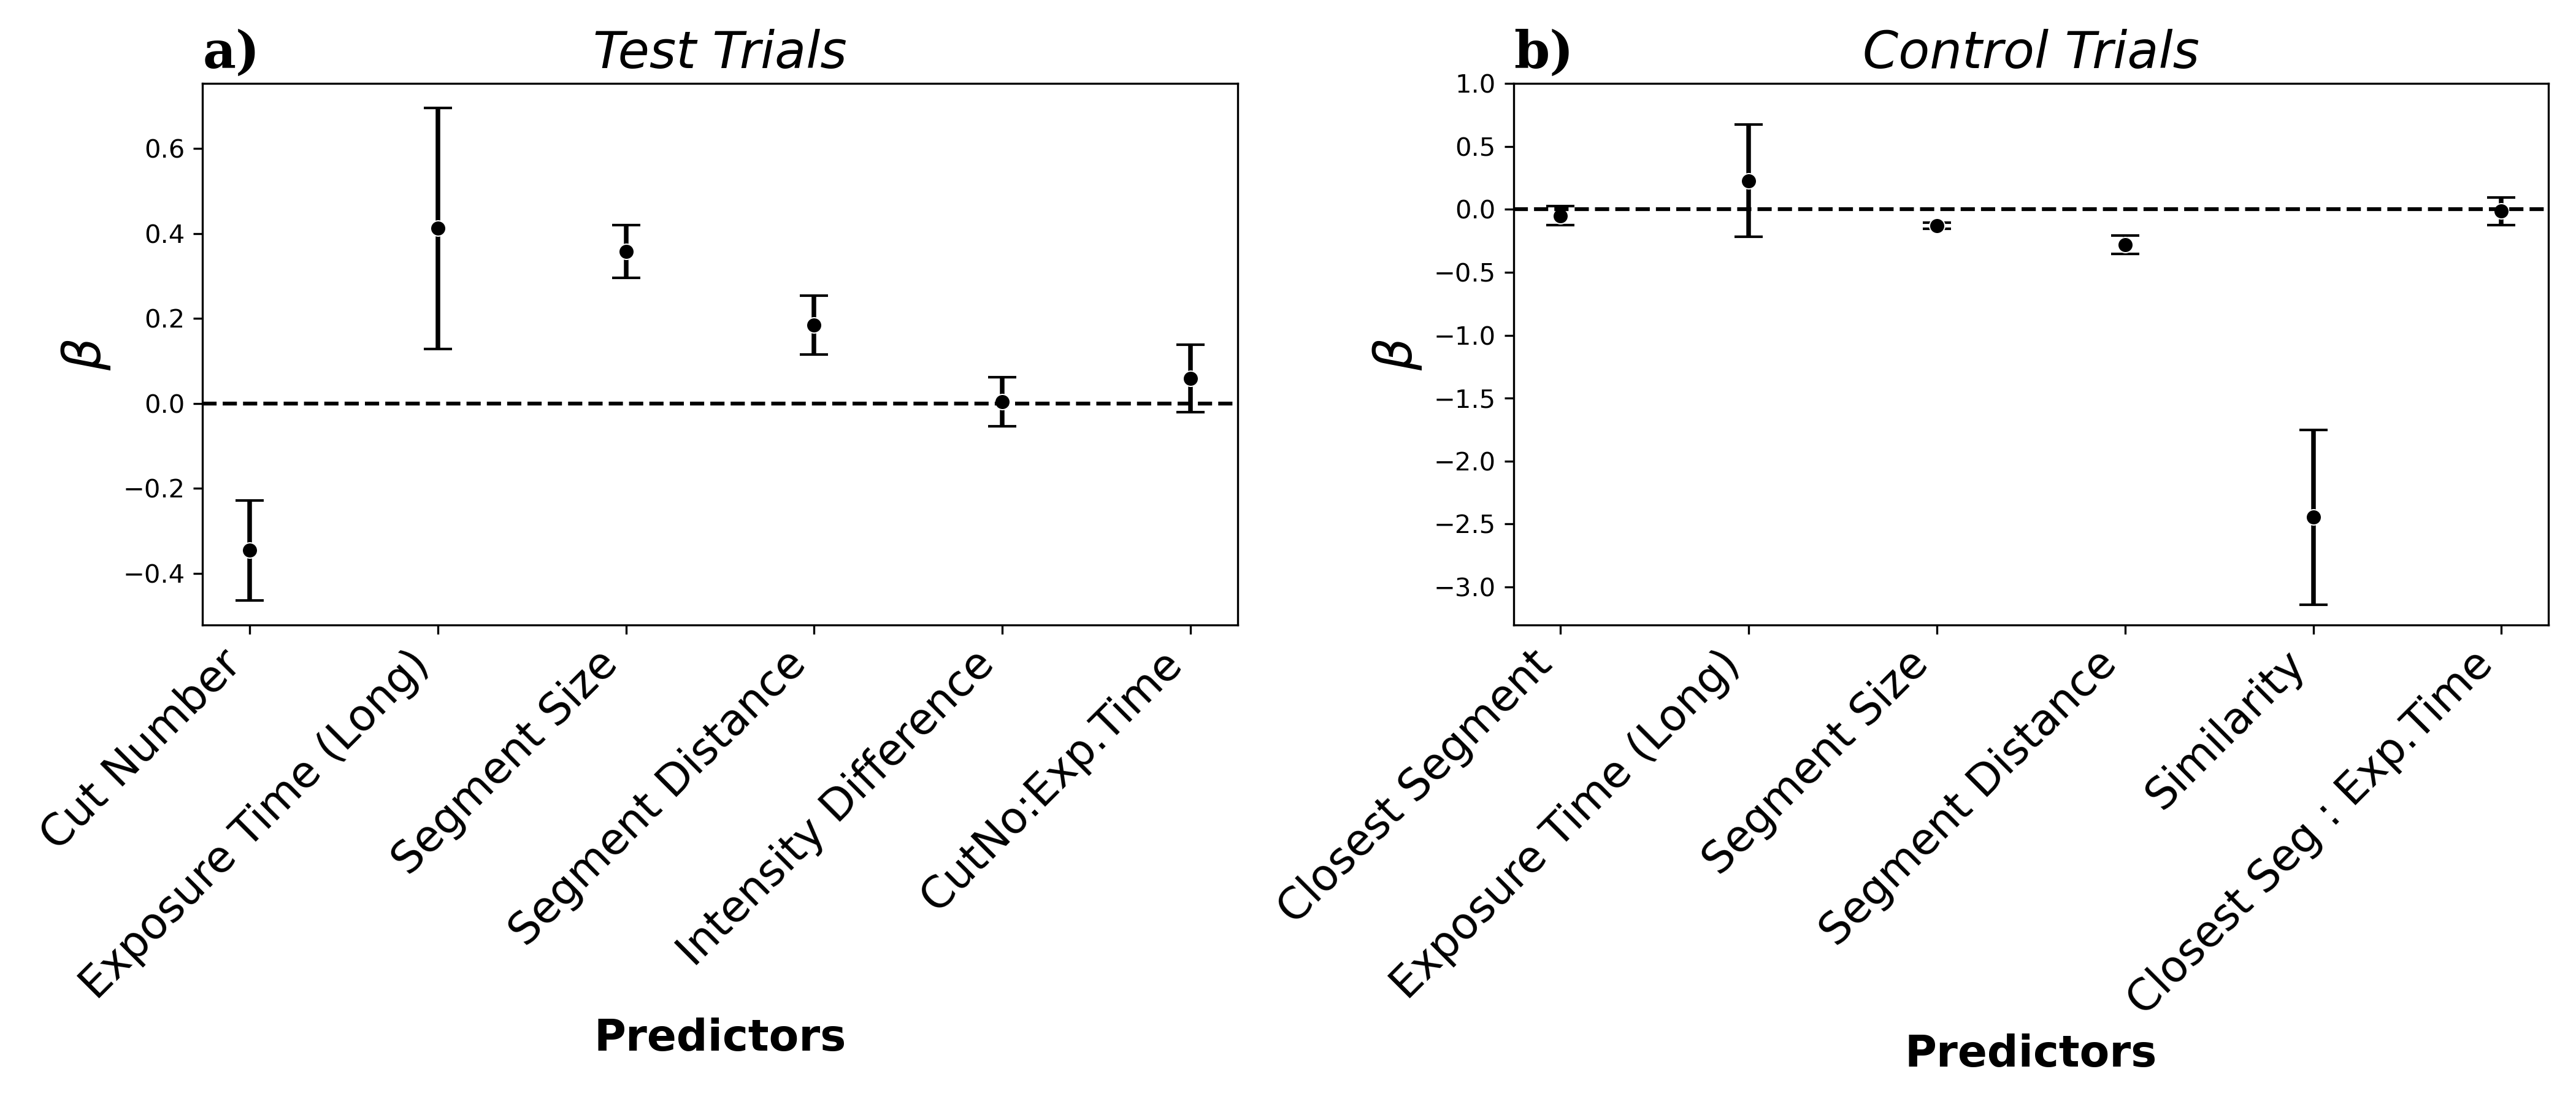
\includegraphics[width=1.2\textwidth]{plots/coefficients_rndInt.png}    
    \caption{$\beta$ coefficients for mixed effect regression models. \textbf{a.} shows coefficients when the model fits only to test trials. Cut no is used as both participant-specific random effect and fixed effect. \textbf{b.} shows coefficients when the model fits only to control trials. Random intercept is used as random effect.}
    \label{fig:coeffs_rndInt}
\end{figure}

The results suggest that participants performed better under the long exposure time condition. Higher accuracies for smaller cut no mean that they found segments coming from early cuts easier in comparison to the segments from later cuts. Significant alternative predictors suggest that farther and larger segments are easier to detect.

We also fit another mixed-effects regression model that used only the control trials to analyze participants' correct answers. In this model, we included a random intercept over participants as a random effect. The fixed predictors included the closest segment's cut no, exposure time, segment size, segment distance, and highest similarity. 

In comparison to the model we used for test trials, segment size ($\beta = -.13, SE = .011, z = -11.5, p < .001$) and segment distance ($\beta = -.28, SE = .038, z = -7.441, p < .001$) showed a negative effect. Border similarity between the closest segment in the image and the presented foil was shown to have the largest negative effect ($\beta = -2.45, SE = .35, z = -6.91, p < .001 $). This means that as the segments look more similar to the closest segment in the image, participant performances dropped.

In order to see the effect of learning or exhaustion across trials, a separate set of mixed effect regression models was constructed with block number as participant-specific random and also independent fixed effect along with the same predictors used in other analyses. Block number did not show a significant effect neither in the test ($\beta = 0.00, SE = .02, z = -.24, p = .81 $) nor in the control trials ($\beta = 0.02, SE = 0.01, z = 1.64, p = .1 $)  suggesting learning across trials did not occur in the experiment (Supplementary Materials \ref{learning}).


\subsection{Fitting Data Using Psychometric Function}
Our regression models were designed to fit data into a function with asymptotes at 0 and 1, which may not be the optimal fit for our data. Since we designed our experiment to capture the perceptual processes, we employed a psychophysical approach that offers more realistic modeling. 

In comparison to regression analyses, the psychophysical approach does not assume fixed a relationship between predictors and the dependent variable and uses non-linear approaches. Additionally, this approach is efficient in computing perceptual parameters like threshold and sensitivity, and provides a better explanation for individual differences. Considering these advantages, the psychophysical approach offers a more accurate and comprehensive understanding of the perceptual processes that occur during visual perception tasks.

We divided our approach into two parts. In the first part, we compare exposure time conditions by fitting the most influential predictors into different psychometric functions. These predictors were cut no, segment size, and segment distance. In the second part, we performed model comparisons across these predictors.

\subsubsection{Comparison of Exposure Times}
\begin{figure}[!hb]
    \centering
    \vspace{-1cm}
    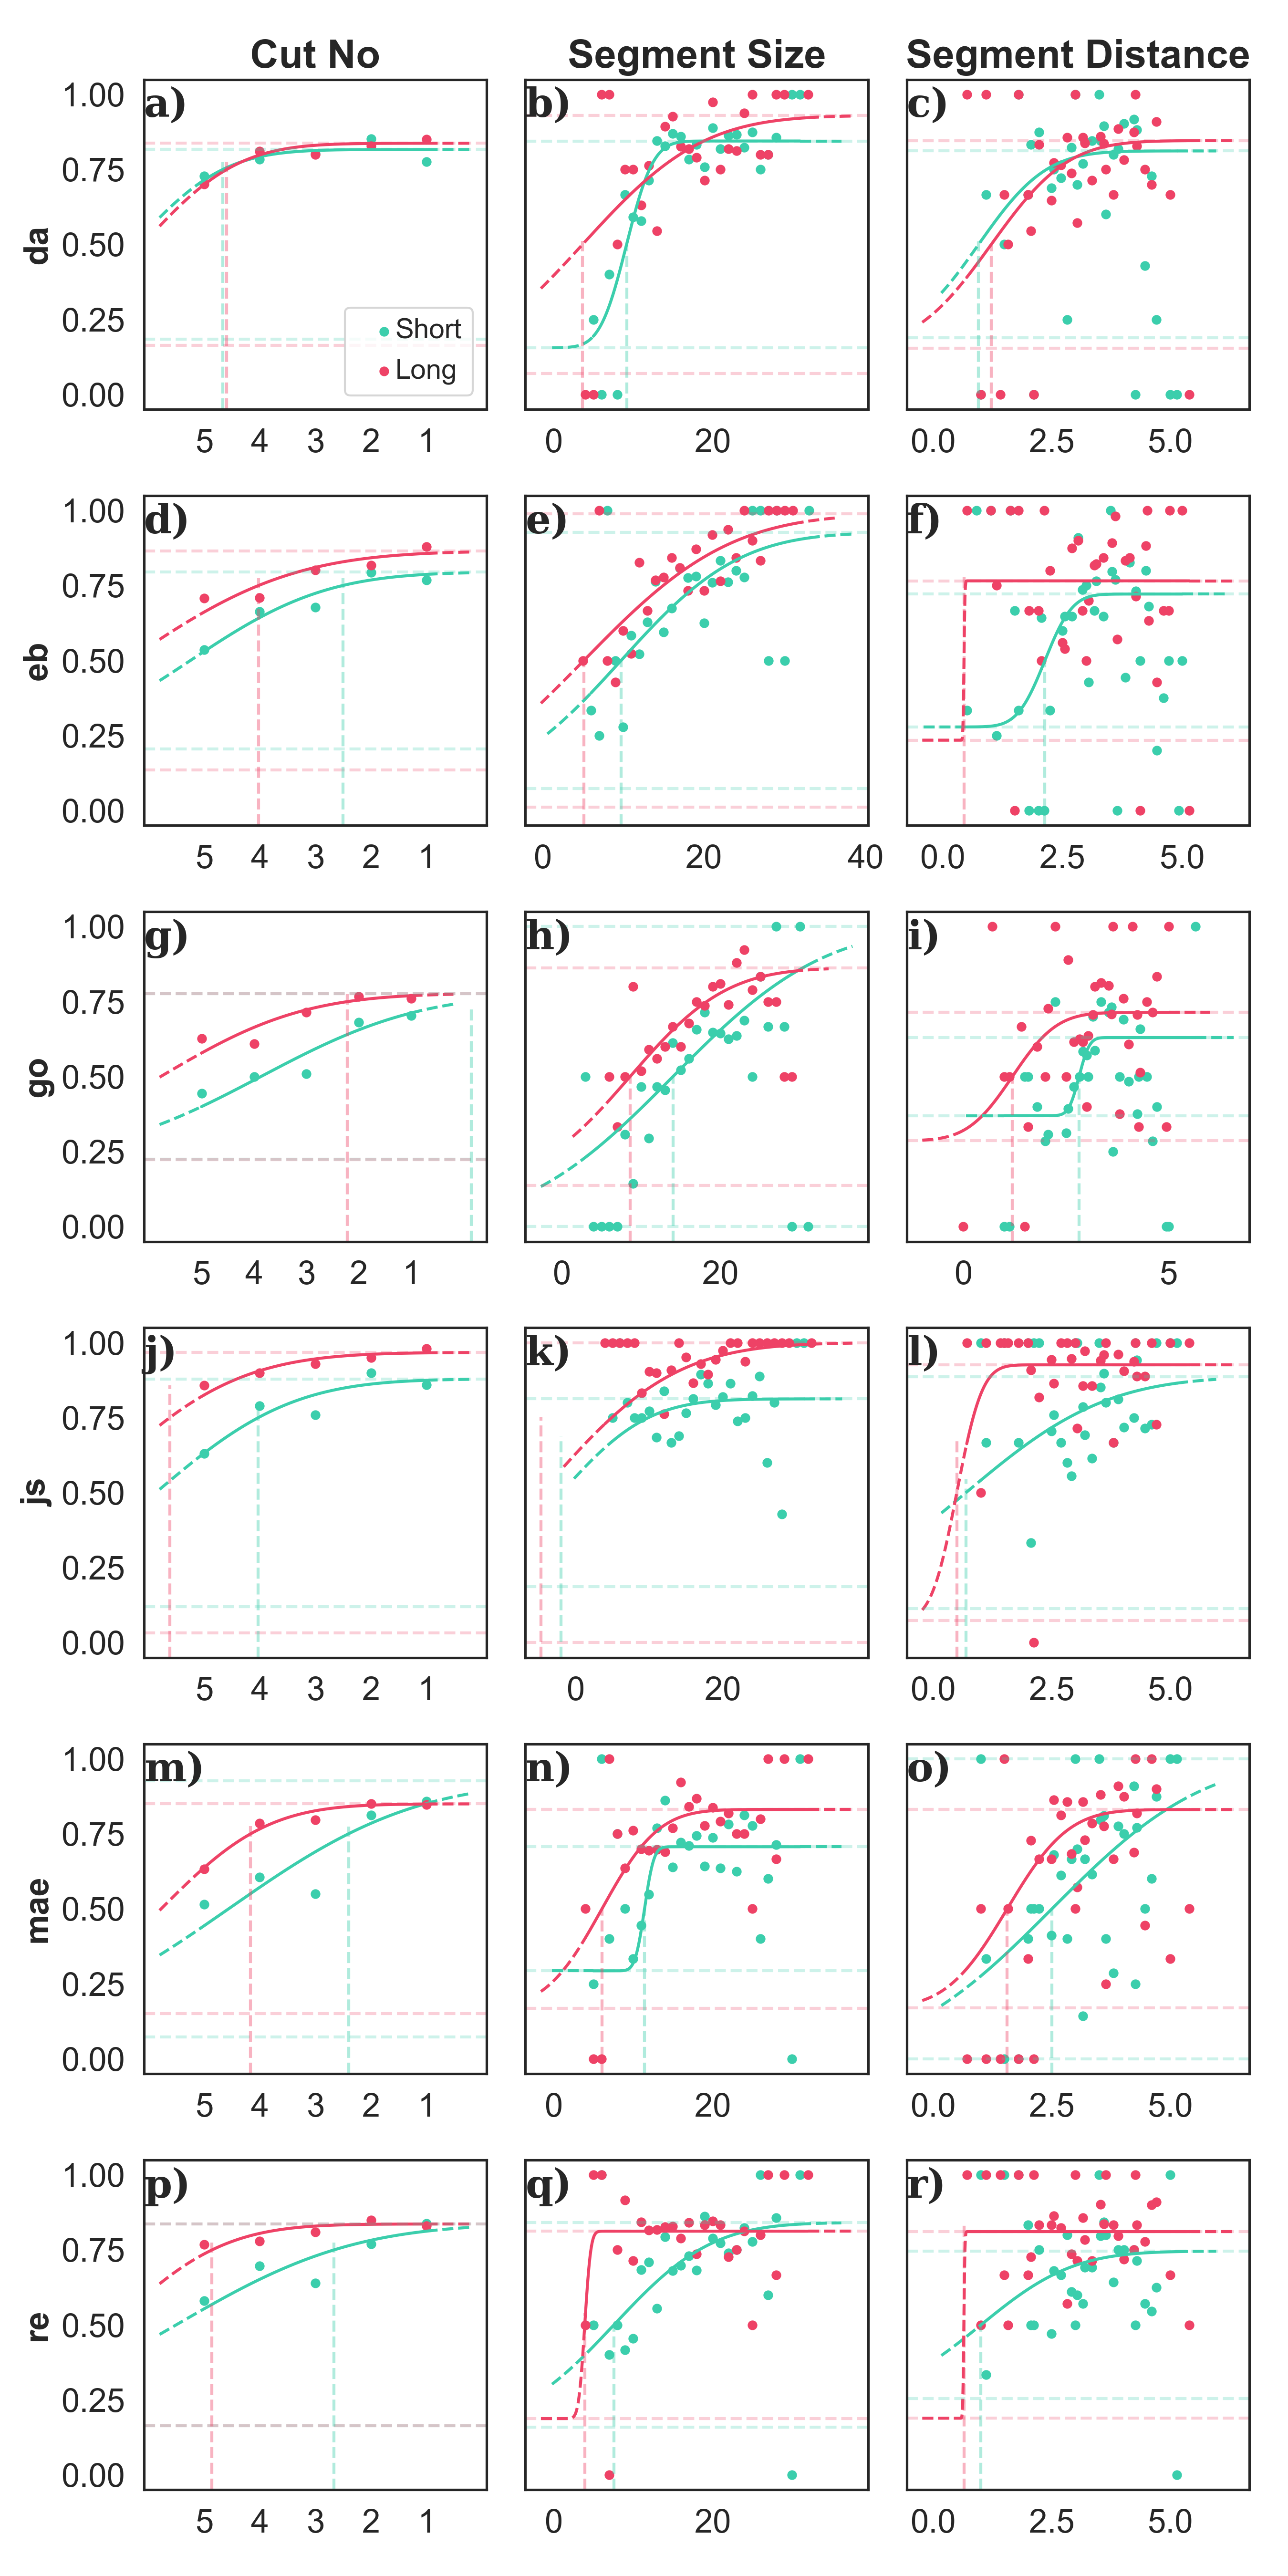
\includegraphics[width = 0.8\textwidth]{plots/psych_fits.png}
    \caption{Psychometric function fits for each predictor across participants. The red line stands for long exposure time, blue line for short exposure time. Vertical lines represent the thresholds. Horizontal lines represent lower and upper asymptotes. The y-axis shows the percent correct. The x-axis shows the stimulus values for each corresponding column. Corresponding goodness of fits for each of the fits can be found under Supplementary Materials  \ref{appendix:gof}}.
    \label{fig:psych_fits}
\end{figure}

To test if there is a difference between exposure time conditions in relation to predictors cut no, segment size, and segment distance; different psychometric function fits were performed. For each predictor, one fit for short and one fit for the long exposure time condition was executed. This procedure was applied to participants separately and completed using Psignifit toolbox for Matlab (\cite{schutt2015psignifit}). Since the accuracy of participants decreases as cut no increases thus it was not possible to fit it to Cumulative Gaussian Distribution, the order of data used for this predictor was reversed. Data was not manipulated for other predictors, and it was fit to Cumulative Gaussian Distribution. $75\%$ accuracy was set as the threshold value for cut no predictor. Since there are cases where upper asymptotes for segment size and segment distance predictors lie below $75\%$ accuracy, $50\%$ was set as the threshold. The same priors were used for all participants. Psychometric functions for these predictors across participants can be seen in Figure \ref{fig:psych_fits} with thresholds and asymptotes for different exposure time conditions.

Psychometric functions show that thresholds for the long exposure time conditions are always lower than the short exposure time condition except for participant \textbf{D.A} (Figure \ref{fig:psych_fits}). These results show that participants were more sensitive to stimulus properties and able to detect the presented segments easier (cut no, segment size, segment distance) in the long exposure time condition than in short condition. All threshold values can be seen in Table \ref{tab:psych_thr}.

\begin{table}[!hb]
    \centering    
    \caption{\textbf{Thresholds for short and long exposure time conditions.}}
    \label{tab:psych_thr}    
    \begin{tabular}{c|ccc}
    \hline
    ID &     Predictor & Short Exp. Time & Long Exp. Time  \\
    \hline    
    D.A. &    Cut No &   1.337748 &  1.407849 \\
    E.B. &     &   3.492886 &  1.978581 \\
    G.O. &     &   6.137583 &  3.779563 \\
    J.S. &     &   1.971463 &  0.381695 \\
    M.A.E. &    &   3.595919 &  1.836959 \\
    R.E. &     &   3.334828 &  1.142791 \\
    \midrule
    D.A. &  Seg. Size &   9.182048 &  3.642508 \\
    E.B. &  &   9.731037 &  5.115287 \\
    G.O. &   &  14.008968 &  8.615146 \\
    J.S. &   &  -1.944792 & -4.698285 \\
    M.A.E. &  &  11.435349 &  6.084914 \\
    R.E. &   &   7.580310 &  3.915072 \\
    \midrule
    D.A. &  Seg. Distance &   0.957261 &  1.225682 \\
    E.B. &   &   2.132436 &  0.442295 \\
    G.O. &   &   2.819398 &  1.194295 \\
    J.S. &   &   0.689212 &  0.496435 \\
    M.A.E. &  &   2.507805 &  1.562439 \\
    R.E. &   &   1.007435 &  0.646122 \\
    \hline
    \end{tabular}
    \captionsetup{labelformat=empty}
    \caption*{\textit{Note:} Results show thresholds for predictors cut no, segment size, and segment distance across participants. Except for D.A., the long exposure time condition has lower threshold than the short exposure time condition. It shows that participants were more sensitive to these stimulus properties when they are exposed to stimulus for a longer period of time.}
\end{table}


In another procedure to test the effect of exposure times on performance, posterior density functions (PDF) from psychometric function fits were utilized (Supplementary Materials \ref{fig:mpd}). We first calculated the probabilities for each data point by applying a discrete integral to the PDFs. For each trial, we retrieved the presented segment's cut no, segment size, and segment distance. Later, we drew corresponding probabilities for these values 1000 times for both short and long-exposure time functions. Afterward, these two probabilities were extracted from each other. 

Results showed that except for \textbf{D.A}, the probability of giving a correct response in the long exposure time condition is higher when the presented segment has the same cut no and segment distance than in the short exposure time condition at least for the $80\%$ of the cases. For segment size, except for \textbf{D.A.} and \textbf{J.S.}, this probability was higher in favor of the long exposure time condition for at least $89\%$ of the drawn samples (see Table \ref{table:sampleRes}). This suggests that exposure times have different fitting results, and they led to performance differences for these predictors.

\setlength{\tabcolsep}{3pt}
\begin{table}
    \centering
    \caption{\textbf{Probabilities showing what percentage of samples differ from each other.}}
    \label{table:sampleRes}
    \begin{tabular}{cccc}
    \hline
    ID &  Cut No &  Seg. Dist &  Seg. Size \\
    \hline
    D.A. &  0.338 &    0.479 &    0.542 \\
    E.B. &  0.877 &    0.918 &    0.929 \\
    G.O. &  0.993 &    0.983 &    0.944 \\
    J.S. &  0.984 &    0.808 &    0.550 \\
    M.A.E. &  0.972 &    0.970 &    0.896 \\
    R.E. &  0.961 &    0.852 &    0.998 \\
    \hline
    \end{tabular}
    \captionsetup{labelformat=empty}
    \caption*{\textit{Note:} Results show percentages of samples in which the long exposure sample is larger than the short exposure sample. 1000 samples were drawn separately for each condition.}
\end{table}


\subsubsection{Comparison of Predictors}
\begin{figure}[!hb]
    \centering
    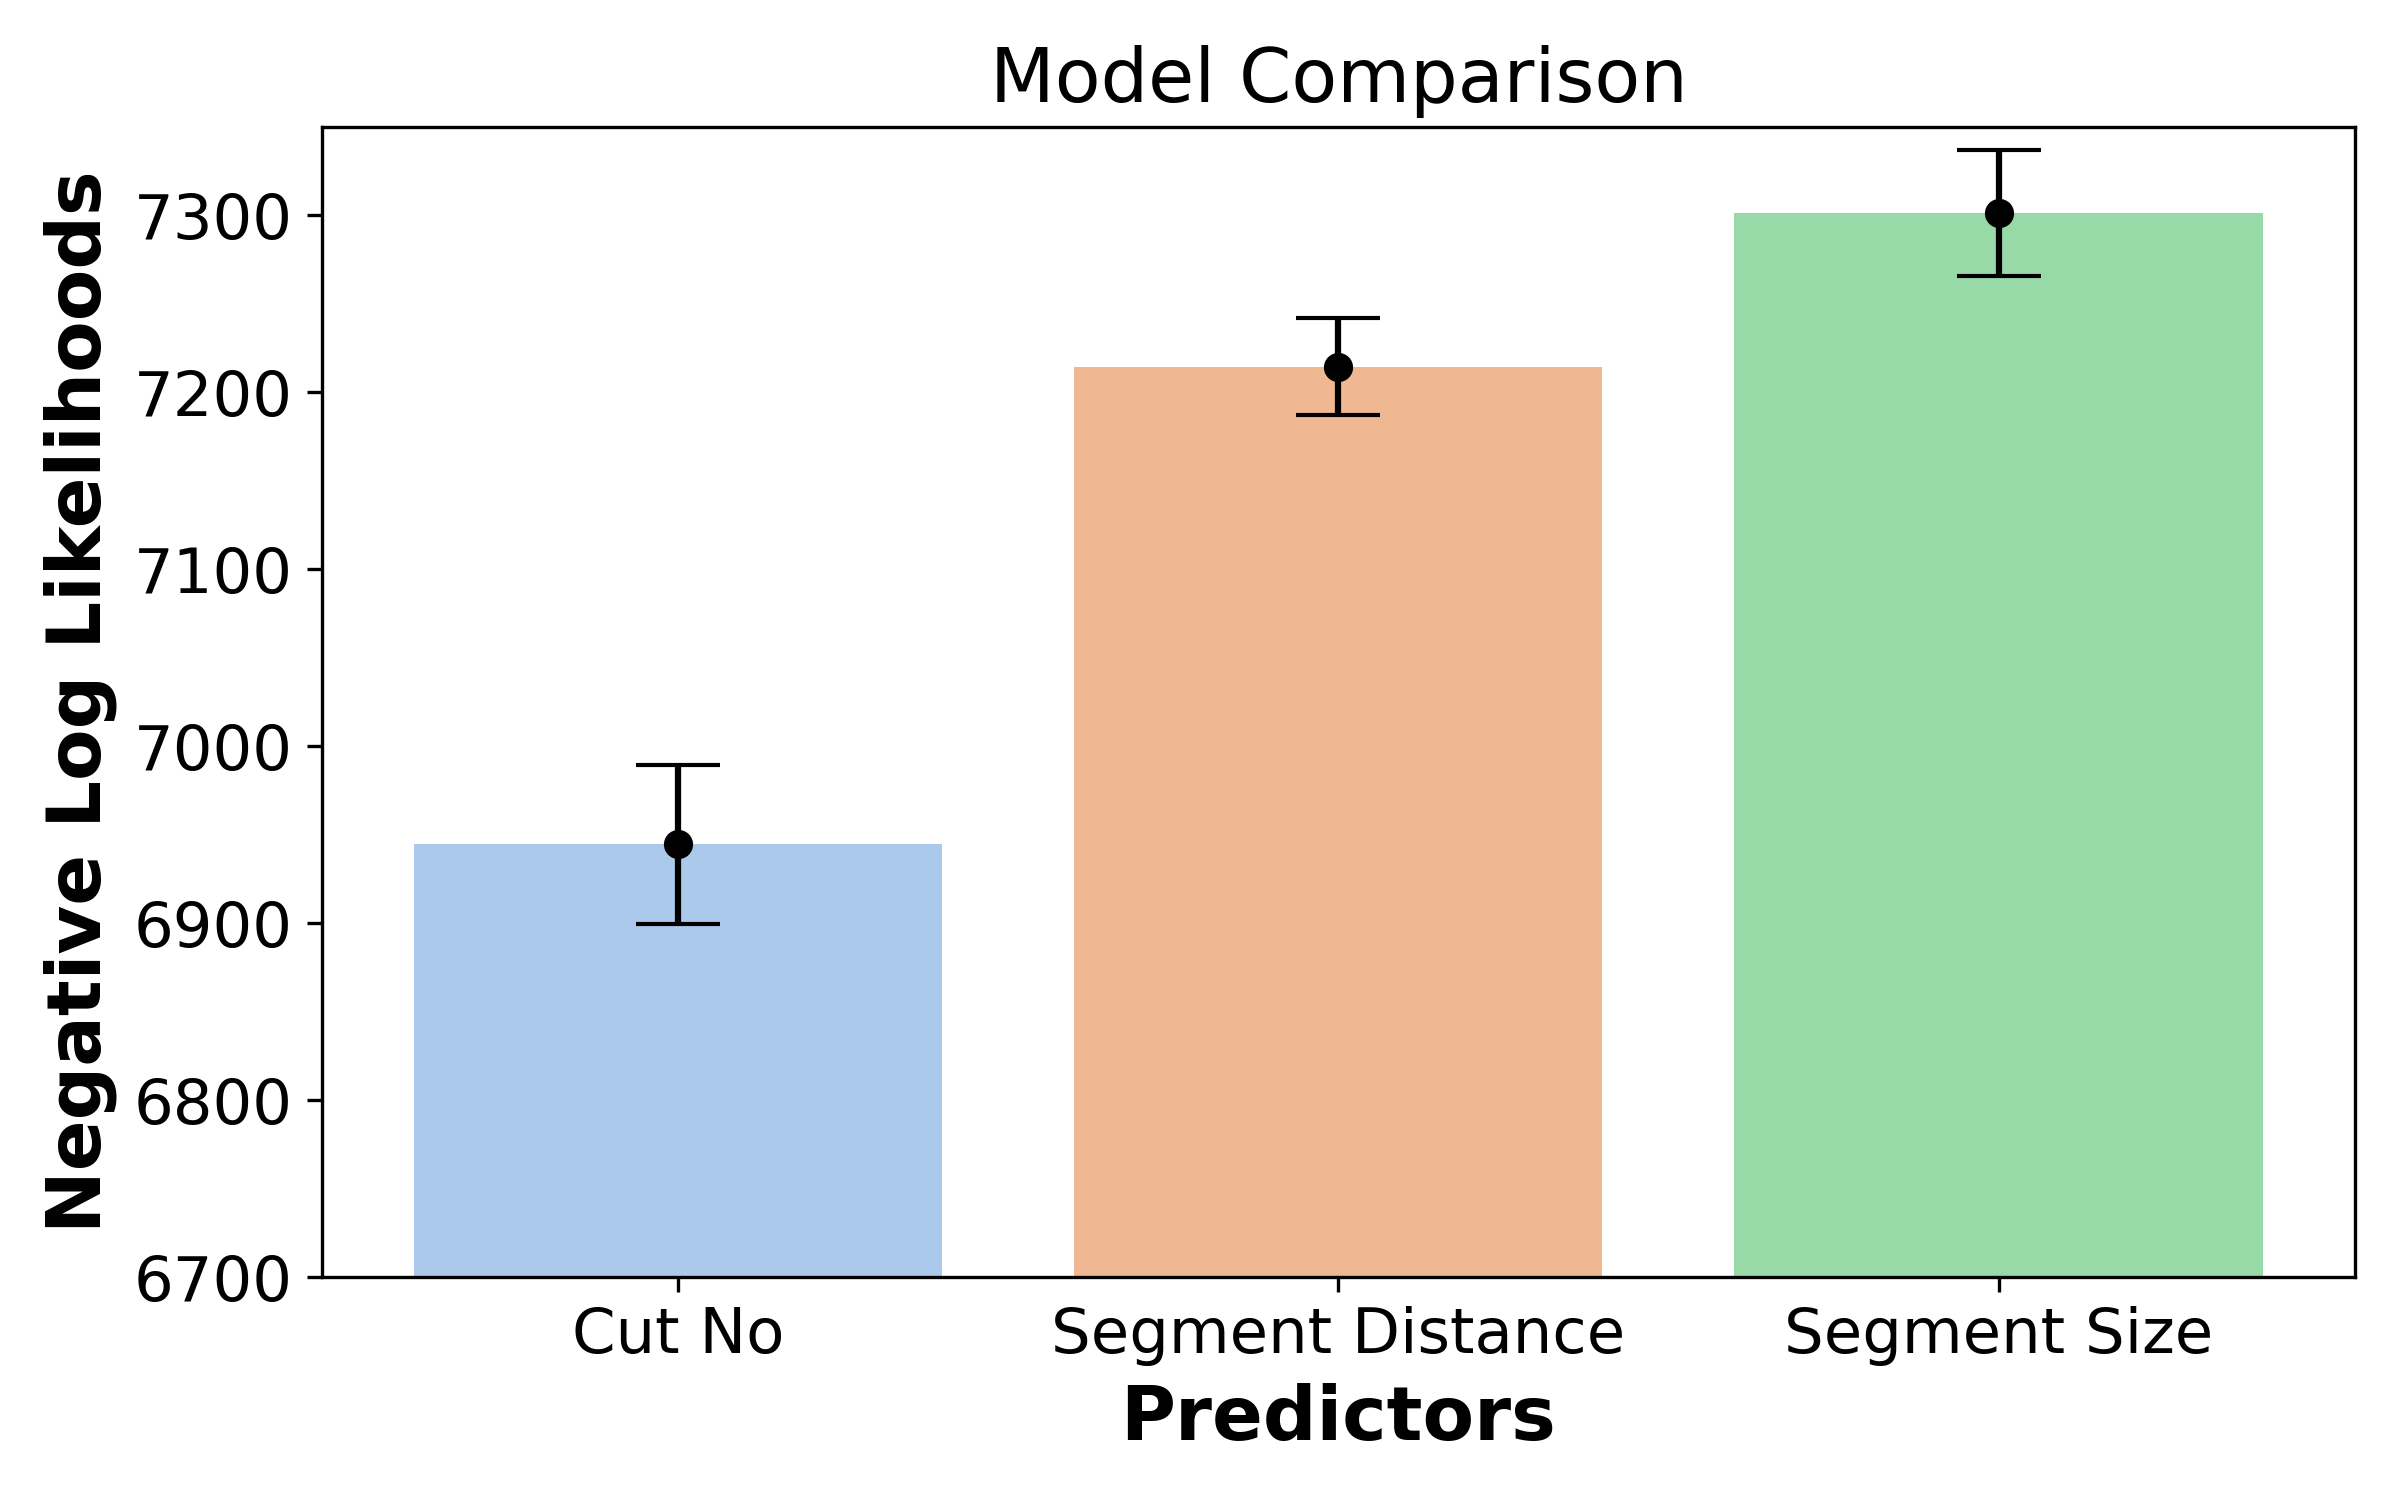
\includegraphics[width=1\textwidth]{plots/psych_modelCompAgg.png}    
    \caption{Model comparison results using negative log-likelihood (NLL) scores. Each bar represents the NLL score for a predictor after they are summed up across participants. Lower scores indicate better predictions. In this analysis, cut no has the lowest score, making it the best predictor. Since the number of parameters is equal across all models, the complexities are also equal, and therefore the NLL scores are proportional to the Akaike Information Criterion (AIC). Due to this relationship, we chose to use NLL scores rather than AIC to simplify the process of comparing models.}
    \label{fig:psych_loglike}
\end{figure}

In the second part of the analysis, we compared various models built using different predictors. Since the number of data points used to fit psychometric functions differed for each predictor, we calculated the negative log-likelihoods on a trial-by-trial basis. For each trial, we obtained its likelihood using the corresponding psychometric function. For the incorrect responses, we subtracted this value from 1 to obtain incorrect response probability. After converting this value to the logarithmic scale, we summed up all the values and multiplied the sum by -1 to obtain a negative likelihood. Later, we summed up values across participants to compute total negative log-likelihood.

Results show that cut no has the lowest negative log-likelihood (Figure \ref{fig:psych_loglike}). Therefore, as we predicted, cut no is the best predictor of participant performance.

\clearpage

\section{Discussion}
Visual perceptual grouping is a fundamental process in the human visual system that enables us to group different visual elements into a single object or group. Understanding how this process works can provide insights into how our brains process and interpret visual information. In this study, we investigated whether visual grouping has a hierarchical basis and whether the level of segmentation depends on the time that people are exposed to stimuli. Furthermore, we wanted to approximate hierarchical grouping behavior by modeling through the normalized min-cut algorithm (\cite{RN165}).

Our findings suggest that cut no is the determining factor of the performance, which could indicate that there is a hierarchical order in the visual perceptual grouping mechanisms. When cut no was compared to segment size and segment distance, it predicted the participant performance better (Figure \ref{fig:psych_loglike}). Our results are also in line with \citeauthor{RN231}'s idea suggesting that we decompose the perceived image rather than building it up after detecting the finer parts (\citeyear{RN231}). If observer could detect the segments from the leaf nodes of a hierarchical tree with limited computational resources, performance at higher cut no would be higher in the short exposure time condition (Figure \ref{fig:behav_test}). Further, we observe that performance decreases as the cut no increases (Table \ref{fig:glm_coeffs}). Therefore, we provide a constraint that future computational models dealing with visual grouping behavior should take hierarchies into consideration. Additionally, as we observed the positive effect of exposure time over performance (Figure \ref{fig:behav_test}), we suggest that further modeling efforts should also consider the effect of duration. Overall, even though our results do not prove that there is a hierarchical order in the visual perceptual grouping mechanisms, there is a correlation between the level of segmentation and performance. 

One of the reasons behind our choice of normalized min-cut algorithm (\cite{RN165}), was due to its consideration of Gestalt principles. By taking stimulus features and spatial distance between visual elements into consideration, this algorithm is able to perform visual perceptual grouping similar to these principles. In our regression analyses, we found segment distance to be significant, which can be attributed to the algorithm's negative correlation between cut no and segment distance (Supplementary Materials \ref{multicol}). As a segment's distance from the center of the image increases, it is likely to be farther from other segments in the image, resulting in larger spatial distances between nodes across segments and smaller weights between them (see \ref{eq:weight}). The normalized min-cut algorithm aims to find the most dissimilar parts of a graph, so parts of the image with smaller weights are cut earlier. Since the performance at smaller cut no is higher, the detection of these segments easier. Thus, segment distance might have played an indirect role in participant performances.

The performance comparison between test and control trials suggests that different computations may occur behind these procedures. First of all, overall participant performance was higher in control trials (Figure \ref{fig:behav_control}). It suggests that participants were able to detect if the presented segment was not a part of the tested image. Also, neither the closest segment's cut no nor the exposure time did not exhibit any significant effects on accuracy in this trial type. Furthermore, when we look at the regression results, we observe that while segment size and segment distance have positive $\beta$ coefficients in test trials, it is the opposite for control trials. It means that when the presented foil is smaller and closer to the center of the image, performance increases. One potential reason for the discrepancy between test and control trials could be the specificity of the segments. As the size of the foils increases, segments become less specific. Hence, it bears more resemblance to the segments in the image. To test this hypothesis, we conducted another mixed-effect regression model using segment distance, segment size, and trial type to predict key presses (Supplementary Materials \ref{table:keyPress}). Results exhibited that as the segment distance and size increased, participants pressed the "yes" buttons more both in test and control trials. It proves that participants thought that they had seen the target segment or foil in the image when the target was smaller in size and placed further.


One potential critique of our experimental design is that the order of cut nos is determined by the algorithm. This might have helped participants by allowing them to discern the algorithm's approach. We tried to tackle this problem by providing feedback on participant accuracy only at the end of the blocks. Also, the accuracy of participants did not improve across blocks, indicating that learning was shown not significant (Supplementary Materials \ref{learning}). However, future studies could mitigate this limitation by assigning segment orders using a different algorithm, which would allow for a comparison of segment orders between the normalized min-cut algorithm and other algorithms.

Overall, our study contributes to our understanding of the hierarchical nature of visual perceptual grouping. Using the normalized min-cut algorithm which highly makes use of stimulus features and spatial distance showed that this behavior can be modeled. Further studies could focus on using this approach to segment natural images. Moreover, the use of eye-tracking techniques to understand spatial fixation densities and scan paths can highlight the relationship between hierarchy and eye movements. Further research could also test the effect of aging on exposure time-dependent hierarchical visual grouping. Although the global precedence is not age dependent, it was shown that older people struggle with local information processing (\cite{RN236}). Therefore, investigating this by using a stimulus with multiple hierarchical levels may inform about the cognitive impairment.

\clearpage


\printbibliography
\clearpage

\appendix
\addcontentsline{toc}{section}{Supplementary Materials}
\section*{Supplementary Materials}
\section{Statistical analysis}
Markdown files for the behavioral and modeling analyses can be found under the following links:
\begin{itemize}
    \item Experiments:
    \item Data including the pilot experiments:
    \item Python script for the plots:
    \item Regression analyses:
\end{itemize}
\clearpage

\section{Instructions} \label{Instructions}
On-screen instructions for both the pre-experiment and experimental tasks were provided to participants, presented as a single paragraph in a specified order. Participants were required to press the ENTER key to proceed to the next page after reading each instruction. To ensure clarity, corresponding visuals from the experimental procedures were also included in the instruction pages. During the instruction phase, an experimenter was present in the room to answer any questions and clarify any confusion after participants had read the written instructions. 

\clearpage

\subsection{Pre-experiment Instructions}
Welcome to our experiment!
Each trial starts with a fixation window.
You should look in the middle of the window, at the center point between the four edges.

After the fixation window disappears, an image made of hexagons will appear.
The image contains six groups of hexagons, with varying brightness levels.
After a certain time, the image will disappear.

Response phase starts with a fixation cross.
If you could see 6 different segments in the presented image, please press the "UP" arrow key.
If you could not see all the 6 segments, please press the "DOWN" arrow key.

Please respond as fast as possible.
After you submit your response, fixation cross will change its color to black.
After it disappears, a new trial will begin.


You can start the experiment by pressing ENTER key.
\clearpage

\subsection{Experiment Instructions}
Each trial starts with a fixation window.
You should look in the middle of the window, at the center point between the four edges. After the fixation window disappears, an image made of hexagons will appear.

The image contains six groups of hexagons, with varying brightness levels.
You will be able to look at the image before it disappears, followed by a noisy screen.

In the next step of the experiment, a segment with hexagons will appear.
Your task is to decide if the segment belongs to the image. You can submit your response after the segment disappears.

If you think that the displayed segment belongs to the image, press the "UP" arrow key. If you think that the displayed segment does not belong to the image, press the "DOWN" arrow key.Remember that some of the segments do not belong to the image. Please respond as fast as possible.

After you submit your response, fixation cross will change its color to black. After it disappears, a new trial will begin.

You can start the practice trials by pressing any key.
\clearpage

\section{Pilot experiment}
\label{pilotExp}
Exposure time conditions used in the main experiment followed the results of the preliminary experiments we conducted. In these experiments segments from cut no 2 and cut no 5 were compared across various durations. 

\begin{figure}[hb]
    \centering    
    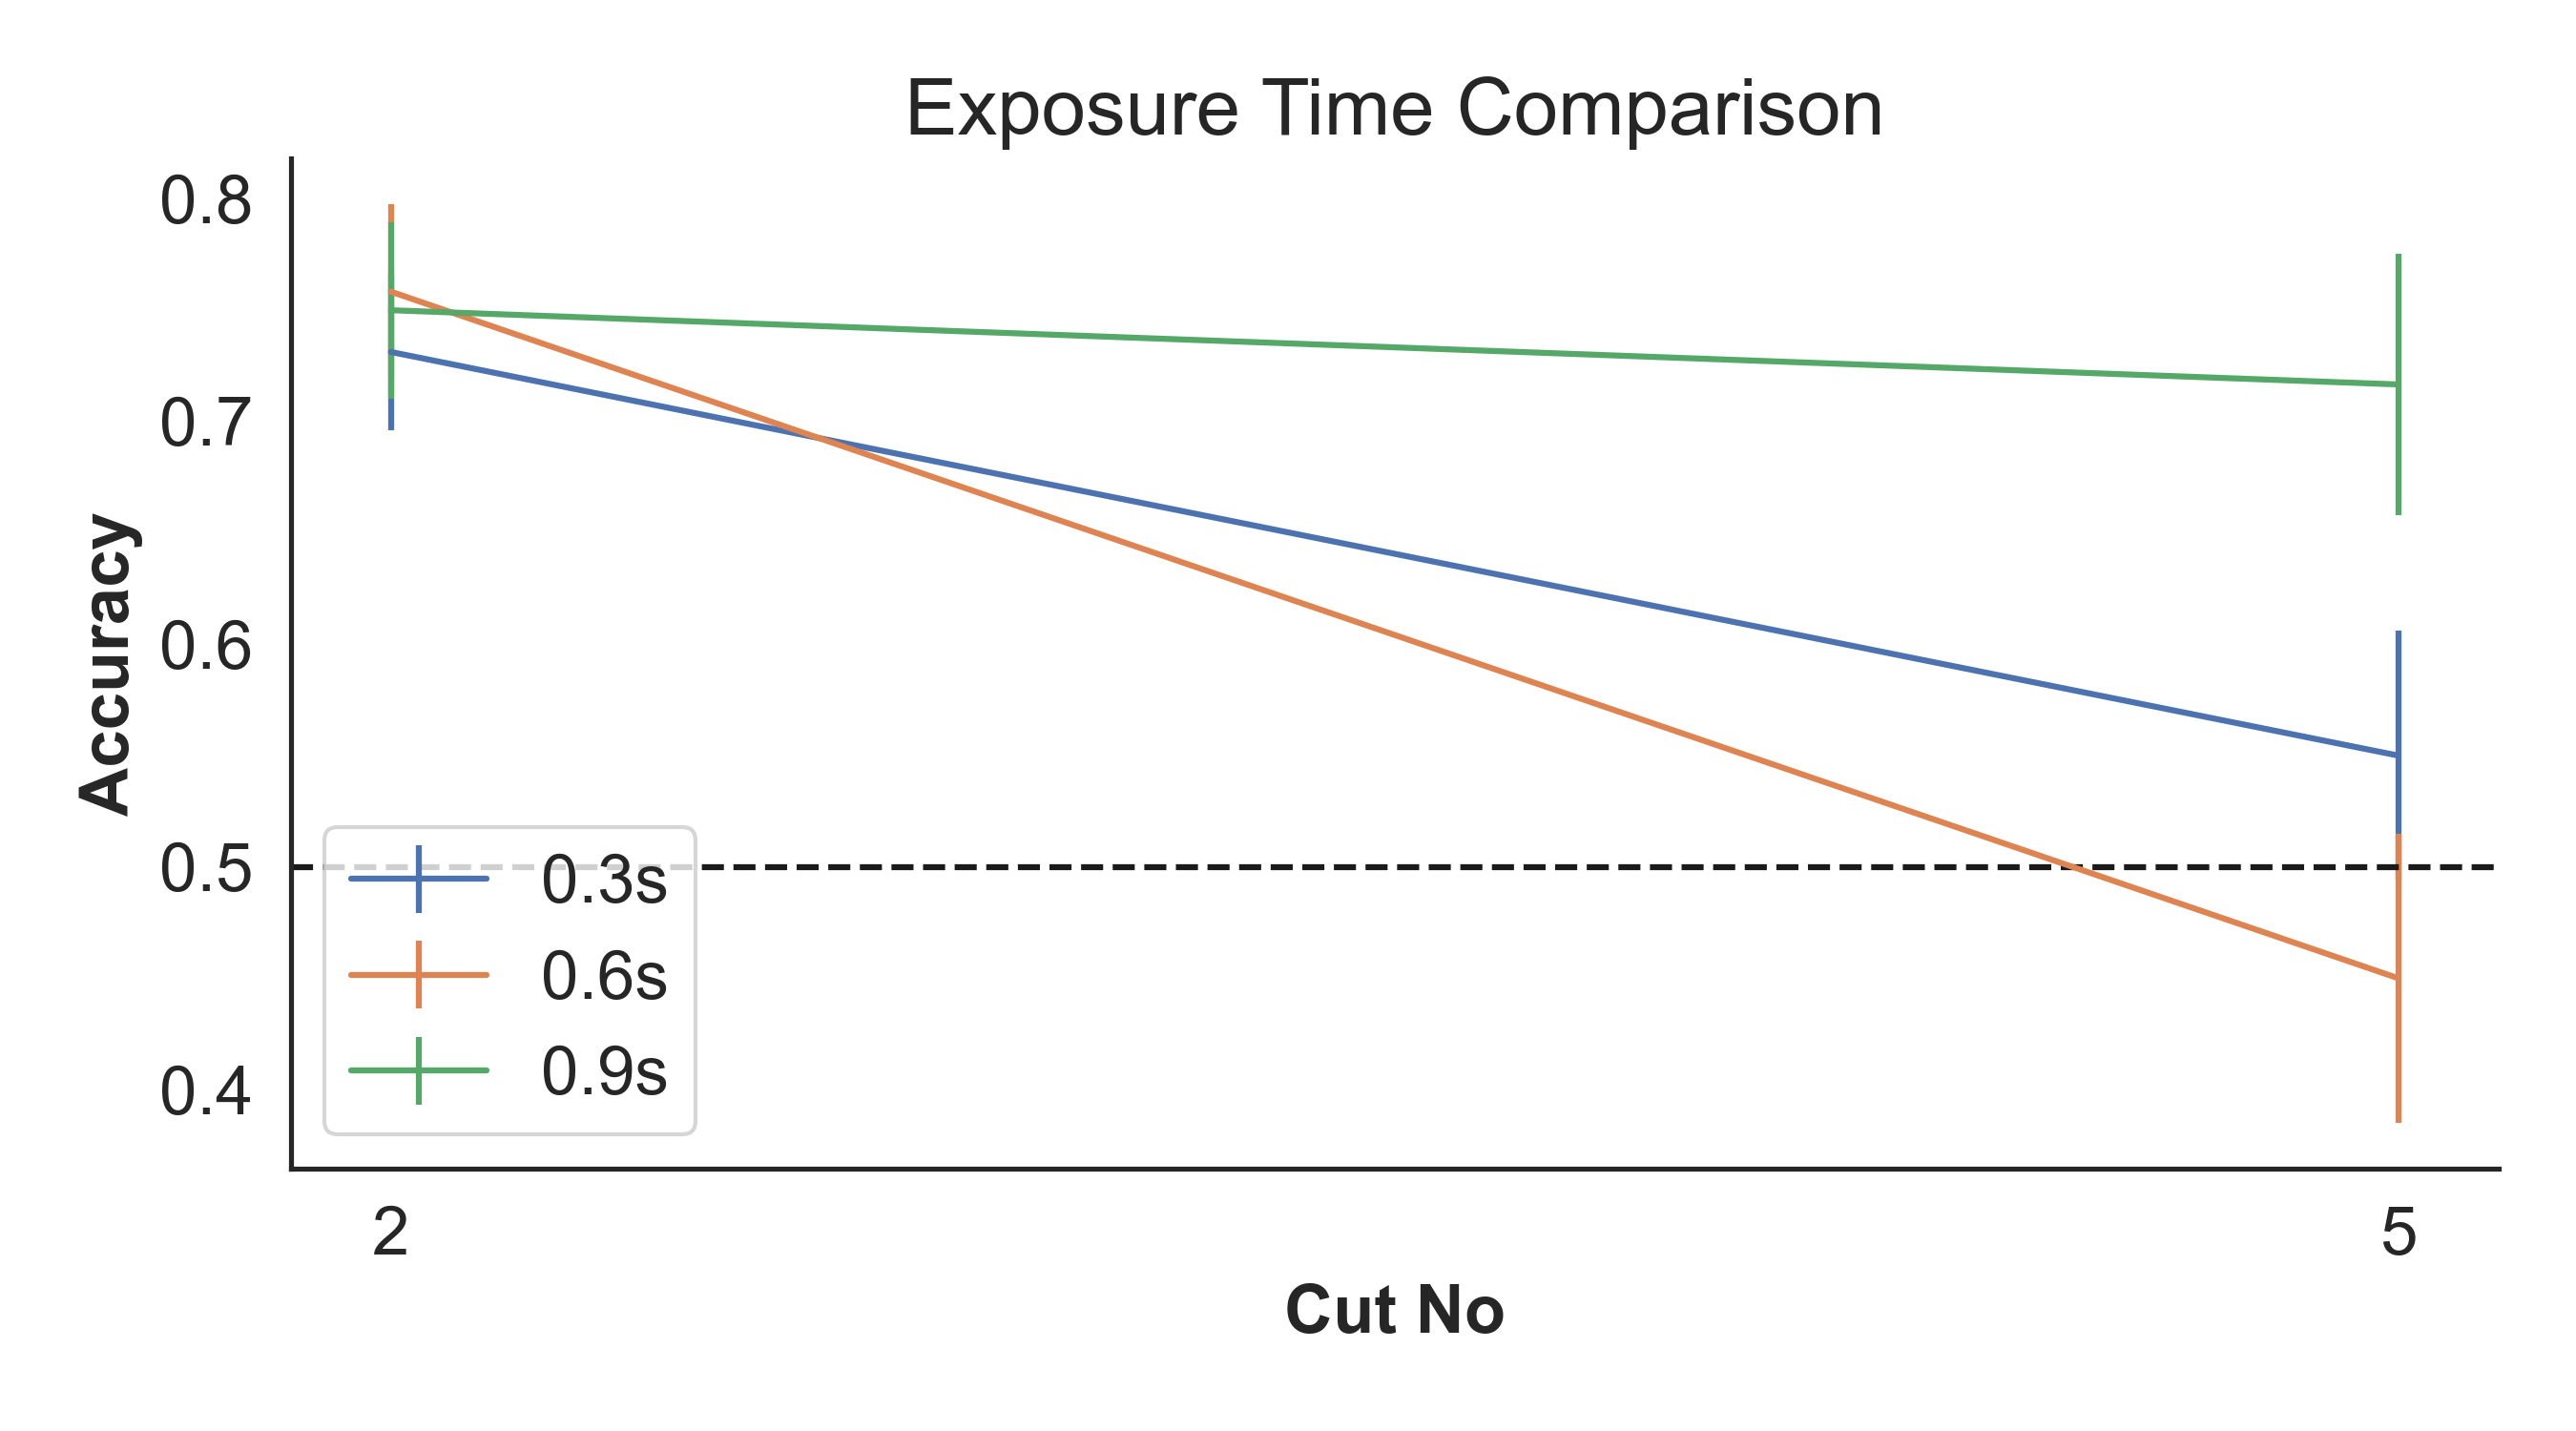
\includegraphics[width = \textwidth]{plots/ExpTimeComparison.png}
    \caption{Comparison of exposure times in the pilot experiments. Error bars represents the standard error of the means. Dotted lines shows the chance level performance. For 0.3 second condition there were 240 trials in total with 160 testing cut no 2 and 80 testing cut no 5. For 0.6 second and 0.9 second conditions, there were 180 trials in total with 120 testing cut no 2 and 60 testing cut no 5 conditions.}
    \label{fig:expTimeComparison}
\end{figure}

\clearpage


\section{Performance across blocks}
\subsection{Regression Results}
In order to test the effect of exhaustion or learning as the experiment progressed, we built separate mixed effect regression models with log-link functions for test and control conditions. Block number was used as participant-specific random and independent fixed effect. We included the same predictors that we used in other regression models.

\textbf{Mixed Effect Regression Results on Test Trials}
\label{table:learningTest}    
\begin{table}[ht]
\centering
\begin{tabular}{rrrrr}
  \hline
 & Estimate & Std. Error & z value & Pr($>$$|$z$|$) \\ 
  \hline
(Intercept) & 1.72 & 0.26 & 6.61 & 0.00 \\ 
  Cut No & -0.35 & 0.06 & -5.83 & 0.00 \\ 
  Exposure Time (Long) & 0.41 & 0.15 & 2.85 & 0.00 \\ 
  Segment Size & 0.36 & 0.03 & 11.41 & 0.00 \\ 
  Segment Distance & 0.19 & 0.04 & 5.29 & 0.00 \\ 
  Intensity Difference & 0.01 & 0.03 & 0.17 & 0.86 \\ 
  Block Number & -0.00 & 0.02 & -0.24 & 0.81 \\ 
  CutNo: ExpTime & 0.06 & 0.04 & 1.48 & 0.14 \\ 
   \hline
\end{tabular}
\end{table}

\textbf{Mixed Effect Regression Results on Control Trials}
\label{table:learningControl}    
\begin{table}[ht]
\centering
\begin{tabular}{rrrrr}
  \hline
 & Estimate & Std. Error & z value & Pr($>$$|$z$|$) \\ 
  \hline
(Intercept) & 4.89 & 0.46 & 10.56 & 0.00 \\ 
  Closest Segment & -0.05 & 0.04 & -1.36 & 0.18 \\ 
  Exposure Time (Long) & 0.22 & 0.23 & 0.97 & 0.33 \\ 
  Segment Size & -0.13 & 0.01 & -11.69 & 0.00 \\ 
  Segment Distance & -0.28 & 0.04 & -7.35 & 0.00 \\ 
  Similarity & -2.45 & 0.36 & -6.88 & 0.00 \\ 
  Block Number & 0.02 & 0.01 & 1.64 & 0.10 \\ 
  Closest Seg.: Exp. Time & -0.01 & 0.06 & -0.23 & 0.82 \\ 
   \hline
\end{tabular}
\end{table}
\clearpage

\subsection{Plots for individual participants}
\label{learning}
\vspace{-0.7cm}
\begin{figure}[!hb]
    \centering
    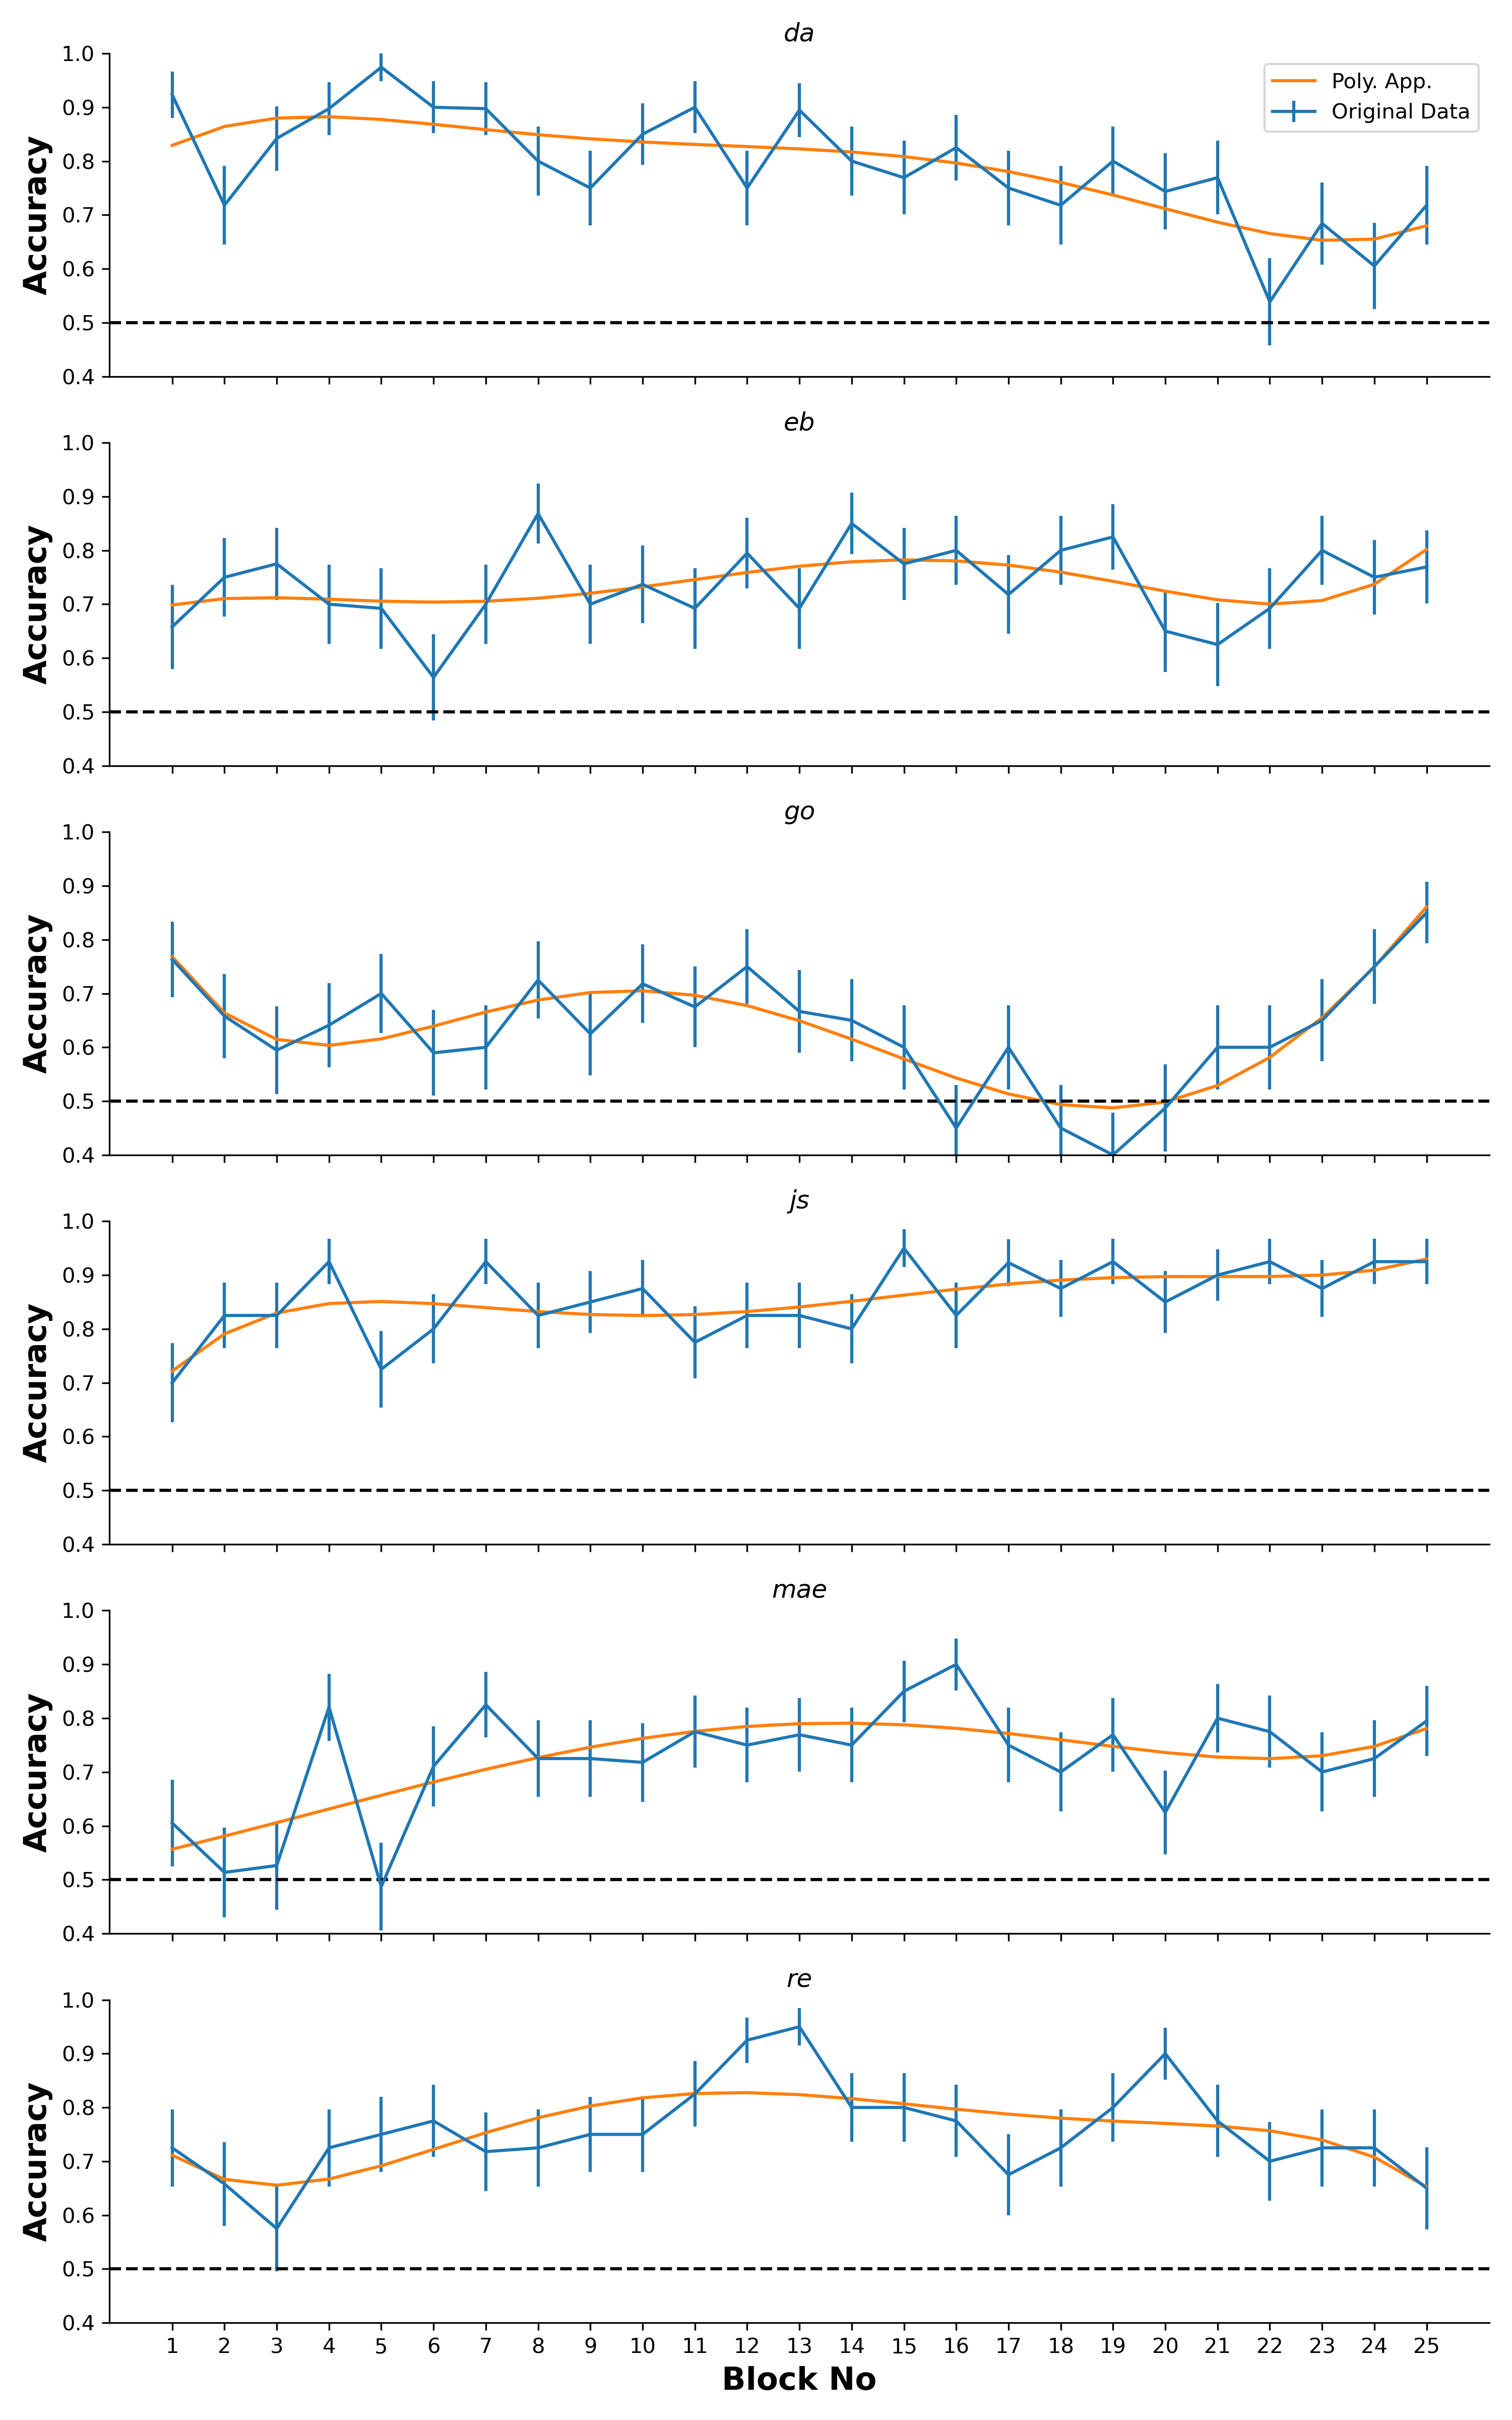
\includegraphics[width = 0.87\textwidth]{plots/learning.png}
    \caption{Figure shows the performance across blocks for each participant. Error bars represent the confidence intervals (95$\%$). Orange line shows the polynomial approximation. }
    \label{fig:learning_curve}
\end{figure}
\clearpage



\section{Multicolinearity tests for regressors}
\label{multicol}
\begin{figure}[!ht]
    \centering
    \begin{subfigure}{\textwidth}
        \centering
        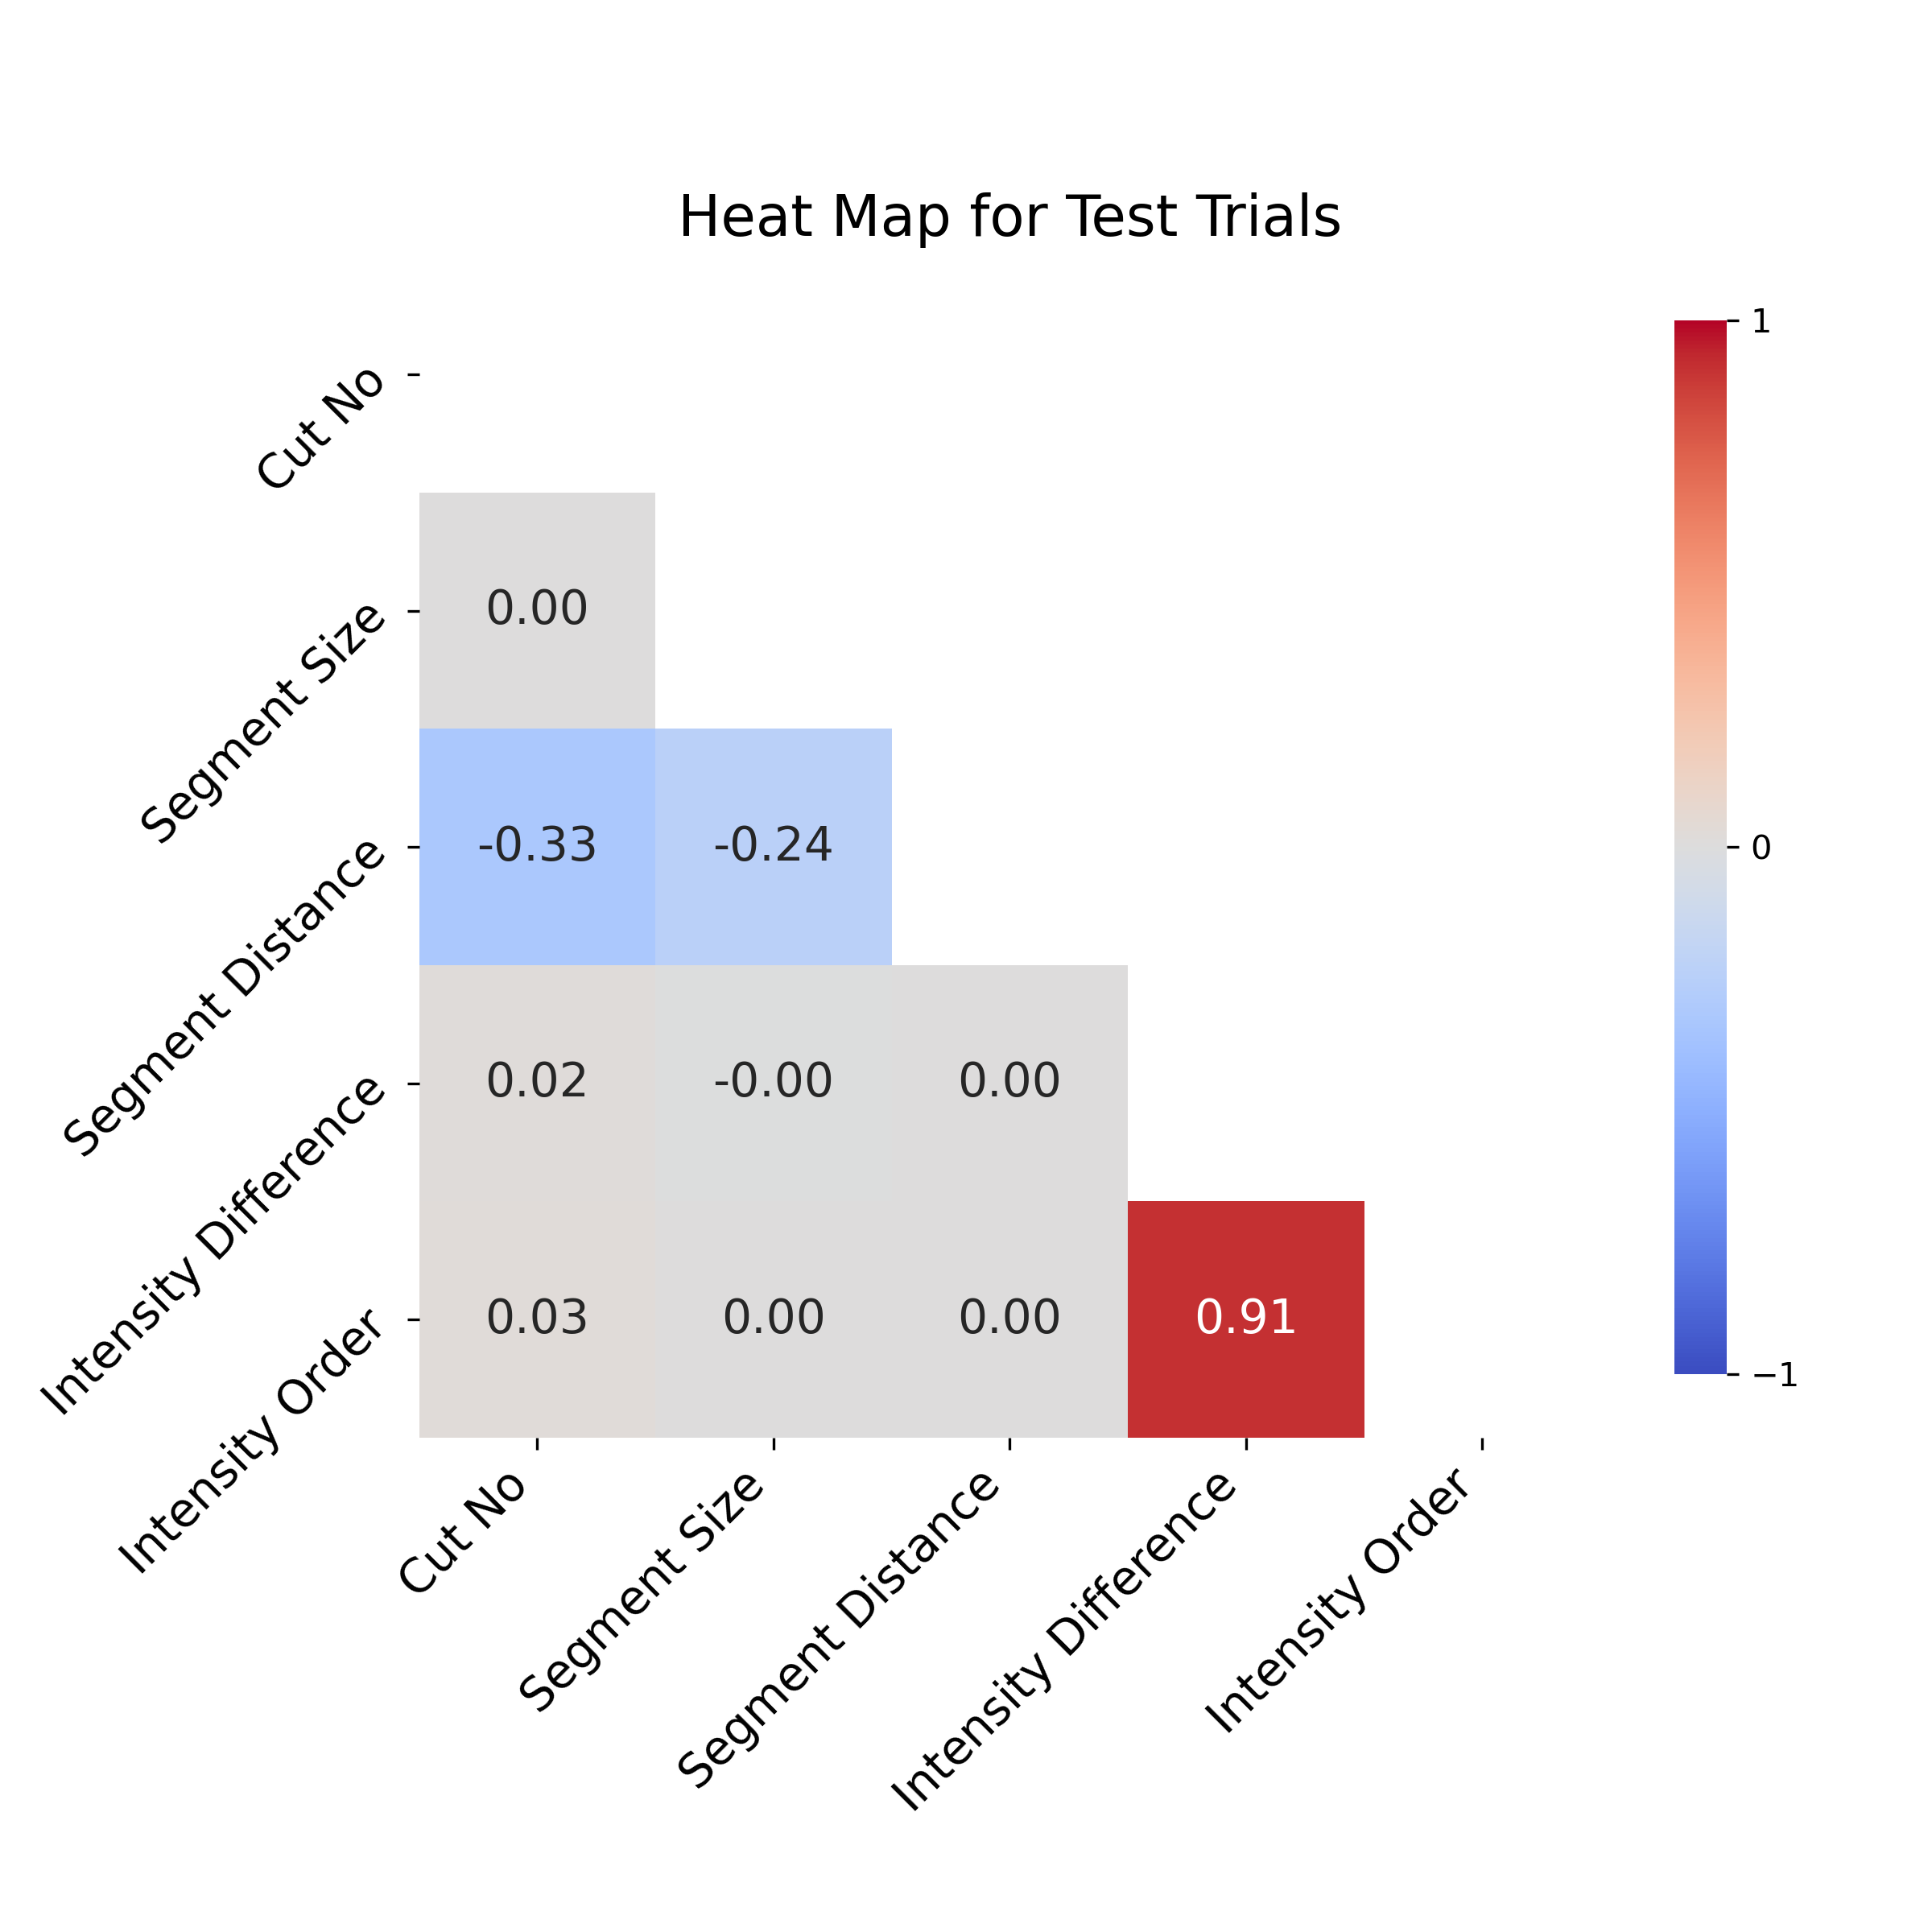
\includegraphics[width = 0.72\linewidth]{Thesis/plots/heatMap_test.png}
        \label{fig:heatmap_test}
    \end{subfigure}
    \hfill
    \vspace*{-1.4cm}
    \begin{subfigure}{\textwidth}
        \centering
        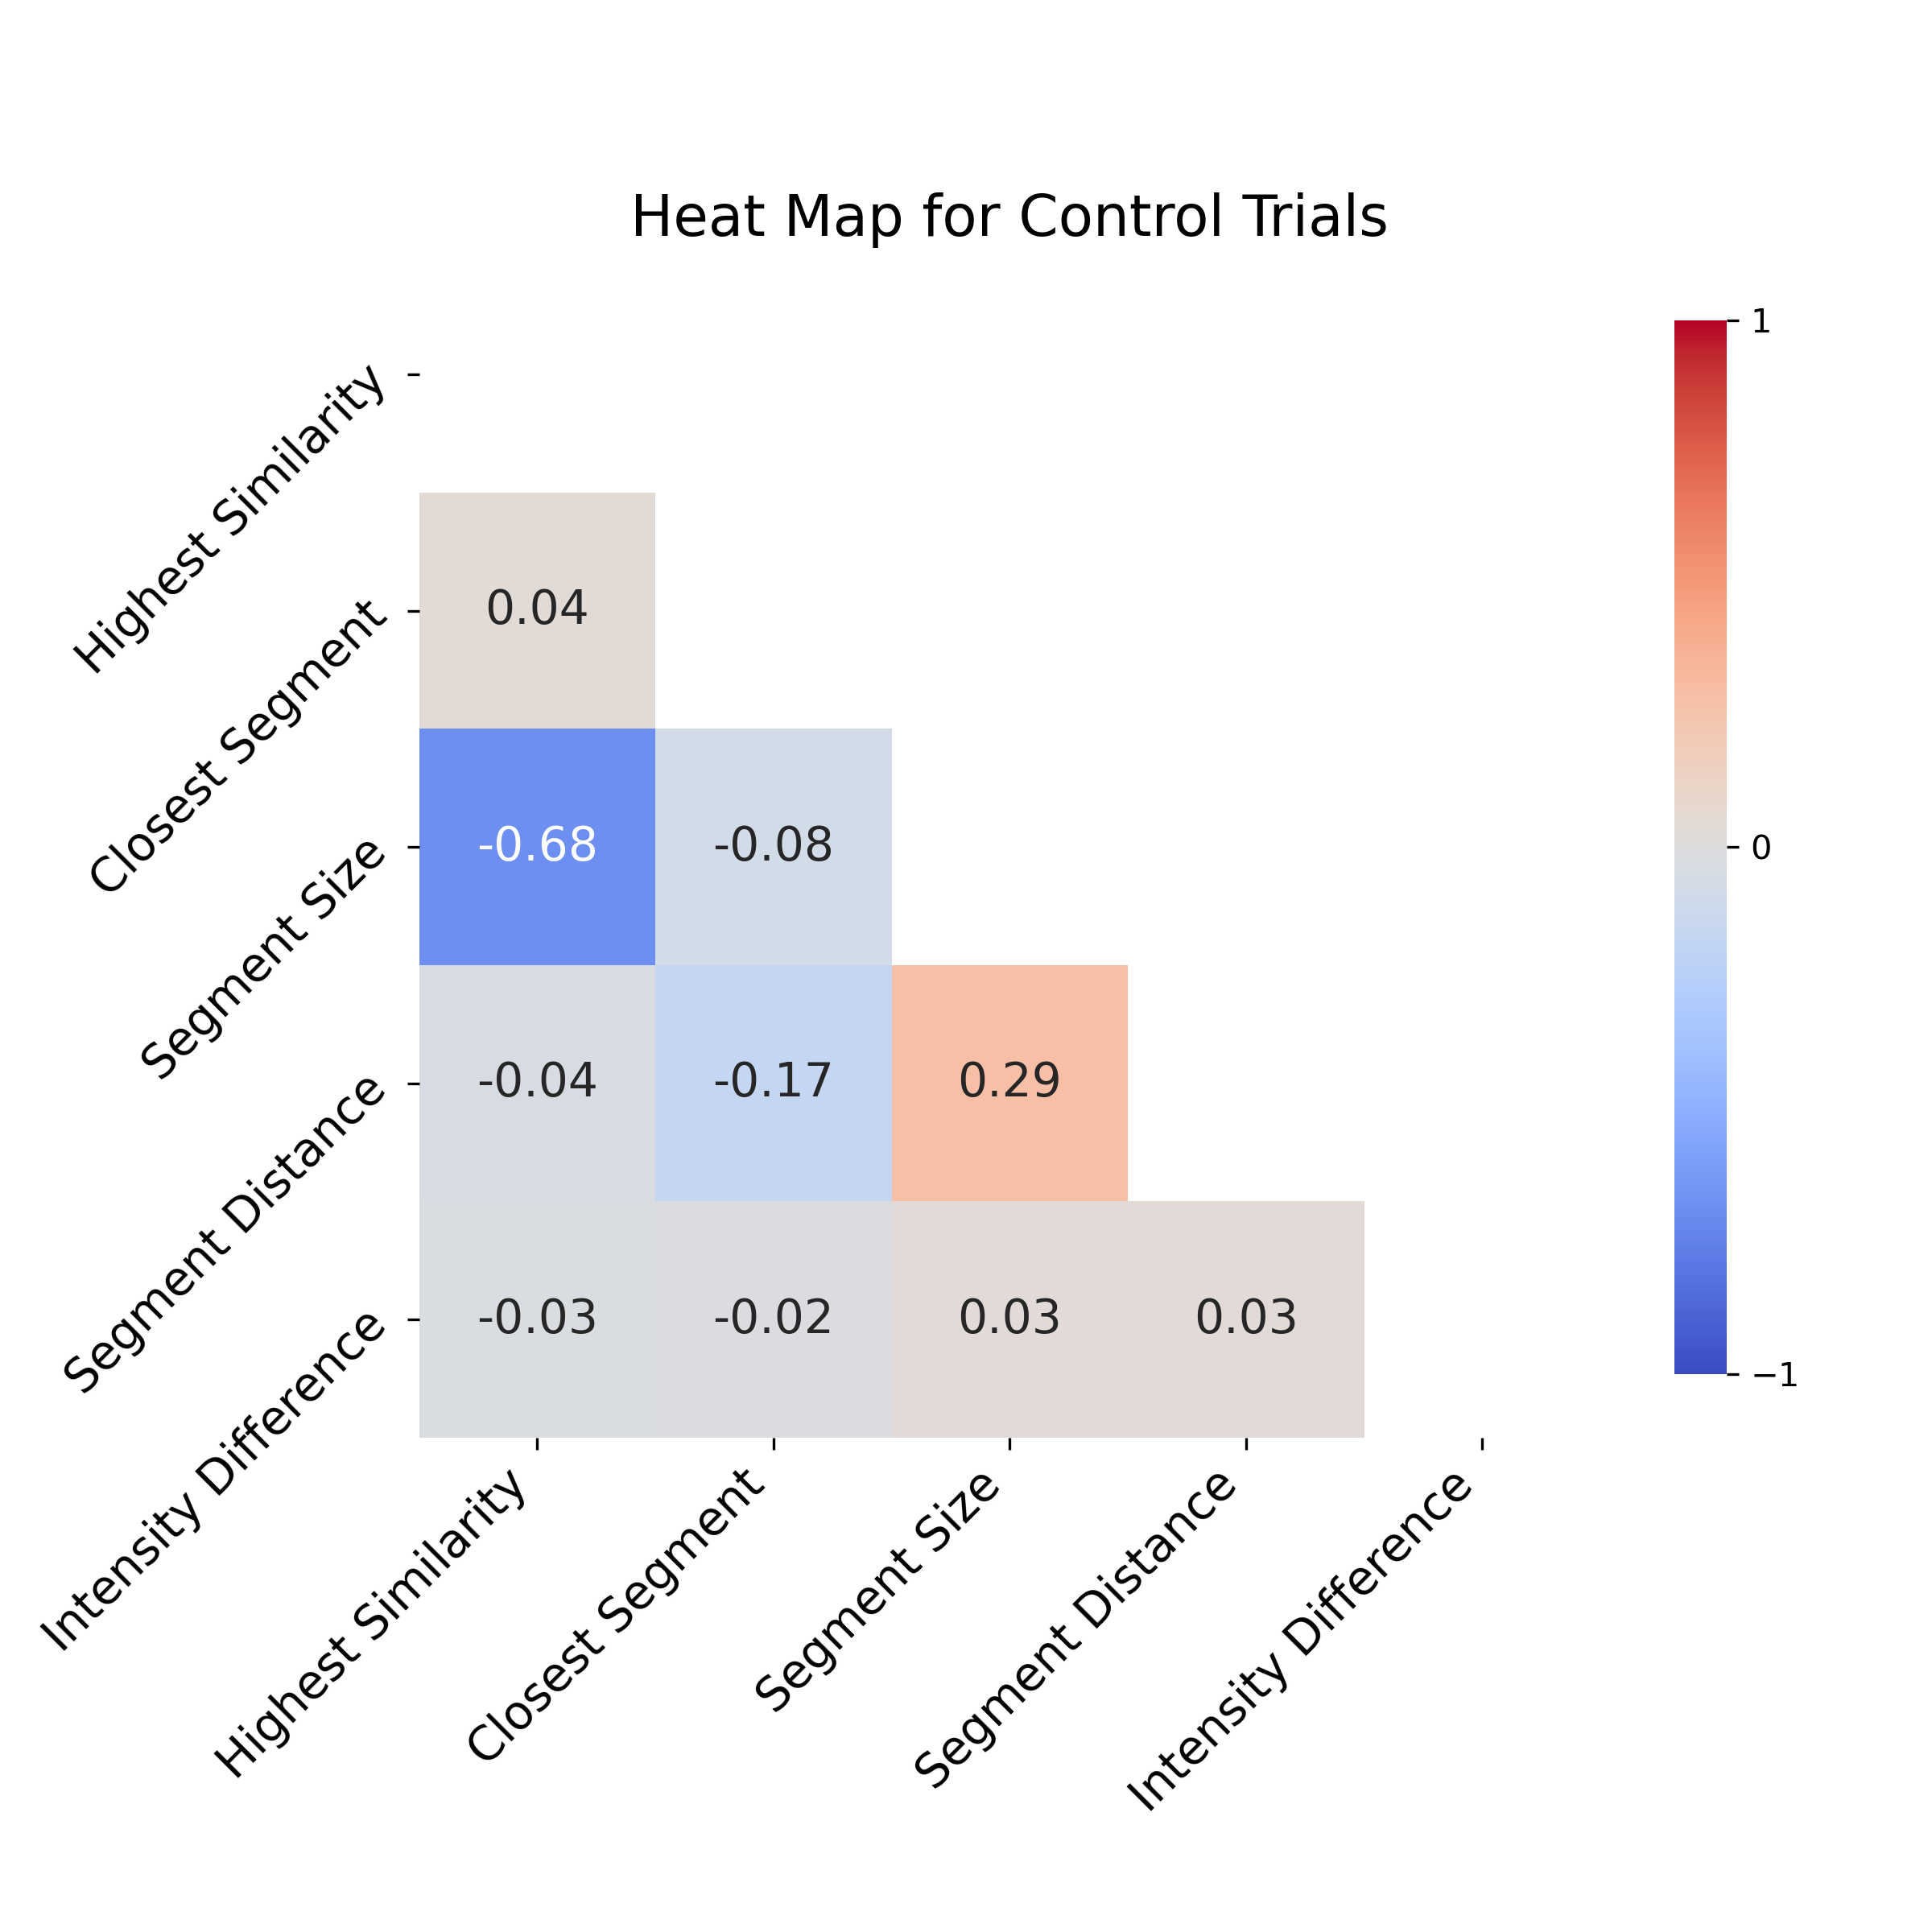
\includegraphics[width = 0.72\linewidth]{Thesis/plots/heatMap_cntrl.png}
        \label{fig:heatmap_control}
    \end{subfigure}
    \label{fig:heatmap}
    \vspace*{-1.7cm}
    \caption{Heatmaps showing the correlations between regressors we used in regression models. Cut no's correlation with segment distance was expected as normalized min-cut algorithm does partitioning by taking spatial distance into consideration.}
\end{figure}
\clearpage

\section{Model comparison results with $\chi^2$ test } \label{participantANOVAs}

Generalized linear models were built to predict accuracy of participants. Model for test trials included the following predictors: exposure time, cut no, segment size, segment distance, intensity difference, intensity order, and cumulative effort. 

For the control trials, cut no was replaced with the closest segment's cut no as predictor. Another predictor used in testing control trials is highest similarity. Other predictors from the test models were kept the same.

Response variable for both test and control trial models was the accuracy of participants, and it was modeled using log-link function. Since participants were tested with their subjective contrast sensitivities, separate regression models were fit for each. 

These models were later compared with increasing number of predictors using $\chi^2$ test to examine how residual deviations changed significantly.

\clearpage

\subsection*{E.B.}
\label{table:participantsAnovaEBTest}    
\textbf{$\chi^2$ test on test trials}
\begin{table}[ht]
    \centering    
    \begin{tabular}{cccccc}
    \hline
    Resid..Df & Resid..Dev &    Df & Deviance & ($p > \chi$) &    Predictor \\
    \hline
          981 &   1135.159 &       &          &            &       Random \\
          980 &   1107.020 & 1.000 &   28.139 &      0.000 &       Cut No \\
          979 &   1095.053 & 1.000 &   11.967 &      0.001 &    Exposure Time \\
          978 &   1095.043 & 1.000 &    0.010 &      0.919 &  Cut No:Time \\
          977 &   1093.503 & 1.000 &    1.540 &      0.215 & Cumulative Effort \\
          976 &   1053.656 & 1.000 &   39.847 &      0.000 &    Segment Size \\
          975 &   1051.030 & 1.000 &    2.627 &      0.105 &    Segment Distance \\
          974 &   1049.110 & 1.000 &    1.919 &      0.166 &   Intensity Difference \\
          973 &   1048.027 & 1.000 &    1.084 &      0.298 &     Intensity Order \\
    \hline
    \end{tabular}    
\end{table}


\textbf{$\chi^2$ test on control trials}
\label{table:participantsAnovaEBControl}    
\begin{table}[ht]
    \centering    
    \begin{tabular}{cccccc}
    \hline
    Resid..Df & Resid..Dev &    Df & Deviance & ($p > \chi$) &    Predictor \\
    \hline
           982 &   1090.471 &       &          &            &             Random \\
      981 &   1085.568 & 1.000 &    4.903 &      0.027 & Highest Similarity \\
      980 &   1085.562 & 1.000 &    0.007 &      0.935 &          Exposure Time \\
      979 &   1053.915 & 1.000 &   31.647 &      0.000 &          Segment Distance \\
      978 &   1047.558 & 1.000 &    6.357 &      0.012 &         Intensity Difference \\
      977 &   1021.460 & 1.000 &   26.099 &      0.000 &          Segment Size \\
    \hline
    \end{tabular}    
\end{table}
\clearpage

\subsection*{G.O.}
\label{table:participantsAnovaGOTest}    
\textbf{$\chi^2$ test on test trials}
 
\begin{table}[ht]
    \centering    
    \begin{tabular}{cccccc}
    \hline
    Resid..Df & Resid..Dev &    Df & Deviance & ($p > \chi$) &    Predictor \\
    \hline
      987 &   1300.425 &       &          &            &       Random \\
      986 &   1273.335 & 1.000 &   27.090 &      0.000 &       Cut No \\
      985 &   1255.301 & 1.000 &   18.034 &      0.000 &    Exposure Time \\
      984 &   1254.449 & 1.000 &    0.852 &      0.356 &  Cut No:Time \\
      983 &   1254.362 & 1.000 &    0.087 &      0.769 & Cum. Effort \\
      982 &   1211.370 & 1.000 &   42.992 &      0.000 &    Segment Size \\
      981 &   1207.808 & 1.000 &    3.562 &      0.059 &    Segment Distance \\
      980 &   1207.710 & 1.000 &    0.097 &      0.755 &   Intensity Difference \\
      979 &   1207.387 & 1.000 &    0.323 &      0.570 &     Intensity Order \\
    \hline
    \end{tabular}    
\end{table}

\label{table:participantsAnovaGOControl}    
\textbf{$\chi^2$ test on control trials}
\begin{table}[ht]
    \centering    
    \begin{tabular}{cccccc}
    \hline
    Resid..Df & Resid..Dev &    Df & Deviance & ($p > \chi$) &    Predictor \\
    \hline
      992 &    707.894 &       &          &            &             Random \\
      991 &    705.960 & 1.000 &    1.934 &      0.164 & Highest Similarity \\
      990 &    705.644 & 1.000 &    0.316 &      0.574 &          Exposure Time \\
      989 &    678.110 & 1.000 &   27.534 &      0.000 &          Segment Distance \\
      988 &    677.540 & 1.000 &    0.571 &      0.450 &         Intensity Difference \\
      987 &    646.575 & 1.000 &   30.964 &      0.000 &          Segment Size \\
    \hline
    \end{tabular}    
\end{table}
\clearpage


\subsection*{M.A.E.}
\label{table:participantsAnovaMAETest}
\textbf{$\chi^2$ test on test trials}
 
\begin{table}[ht]
    \centering
    \begin{tabular}{cccccc}
    \hline
    Resid..Df & Resid..Dev &    Df & Deviance & ($p > \chi$) &    Predictor \\
    \hline
          984 &   1158.935 &       &          &            &       Random \\
          983 &   1110.379 & 1.000 &   48.556 &      0.000 &       Cut No \\
          982 &   1093.275 & 1.000 &   17.104 &      0.000 &    Exposure Time \\
          981 &   1091.952 & 1.000 &    1.323 &      0.250 &  Cut No:Time \\
          980 &   1091.131 & 1.000 &    0.821 &      0.365 & Cumulative Effort \\
          979 &   1077.265 & 1.000 &   13.866 &      0.000 &    Segment Size \\
          978 &   1063.085 & 1.000 &   14.180 &      0.000 &    Segment Distance \\
          977 &   1058.255 & 1.000 &    4.831 &      0.028 &   Intensity Difference \\
          976 &   1055.406 & 1.000 &    2.849 &      0.091 &     Intensity Order \\
    \hline
    \end{tabular}
\end{table}


\textbf{$\chi^2$ test on control trials}
\label{table:participantsAnovaMAEControl}
\begin{table}[ht]
    \centering
    \begin{tabular}{cccccc}
    \hline
    Resid..Df & Resid..Dev &    Df & Deviance & ($p > \chi$) &    Predictor \\
    \hline
        989 &    971.077 &       &          &            &   Random \\
      988 &    969.294 & 1.000 &    1.783 &      0.182 & Highest Similarity \\
      987 &    968.374 & 1.000 &    0.920 &      0.338 &          Exposure Time \\
      986 &    929.415 & 1.000 &   38.959 &      0.000 &          Segment Distance \\
      985 &    929.187 & 1.000 &    0.228 &      0.633 &         Intensity Difference \\
      984 &    906.709 & 1.000 &   22.478 &      0.000 &          Segment Size \\
    \hline
    \end{tabular}
\end{table}
\clearpage


\subsection*{R.E.}
\label{table:participantsAnovaRE}    
\textbf{$\chi^2$ test on test trials}
 
\begin{table}[ht]    
    \centering    
    \begin{tabular}{cccccc}
    \hline
    Resid..Df & Resid..Dev &    Df & Deviance & ($p > \chi$) &    Predictor \\
    \hline
      996 &   1107.353 &       &          &            &       Random \\
      995 &   1090.549 & 1.000 &   16.804 &      0.000 &       Cut No \\
      994 &   1075.998 & 1.000 &   14.551 &      0.000 &    Exposure Time \\
      993 &   1073.688 & 1.000 &    2.311 &      0.129 &  Cut No:Time \\
      992 &   1072.061 & 1.000 &    1.627 &      0.202 & Cumulative Effort \\
      991 &   1062.249 & 1.000 &    9.813 &      0.002 &    Segment Size \\
      990 &   1062.141 & 1.000 &    0.108 &      0.743 &    Segment Distance \\
      989 &   1062.109 & 1.000 &    0.032 &      0.857 &   Intensity Difference \\
      988 &   1061.232 & 1.000 &    0.877 &      0.349 &     Intensity Order \\
    \hline
    \end{tabular}    
\end{table}

\textbf{$\chi^2$ test on control trials}
\label{table:participantsAnovaREControl}    
\begin{table}[ht]    
    \centering    
    \begin{tabular}{cccccc}
    \hline
    Resid..Df & Resid..Dev &    Df & Deviance & ($p > \chi$) &    Predictor \\
    \hline
        993 &   1144.558 &       &          &            &             Random \\
      992 &   1142.893 & 1.000 &    1.665 &      0.197 & Highest Similarity \\
      991 &   1139.555 & 1.000 &    3.339 &      0.068 &          Exposure Time \\
      990 &   1136.395 & 1.000 &    3.160 &      0.075 &          Segment Distance \\
      989 &   1135.794 & 1.000 &    0.602 &      0.438 &         Intensity Difference \\
      988 &   1132.007 & 1.000 &    3.787 &      0.052 &          Segment Size \\
    \hline
    \end{tabular}    
\end{table}
\clearpage

\subsection*{D.A.}
\label{table:participantsAnovaDATest}    
\textbf{$\chi^2$ test for participant D.A.}
 
\begin{table}[ht]
    \centering    
    \begin{tabular}{cccccc}
    \hline
    Resid..Df & Resid..Dev &    Df & Deviance & ($p > \chi$) &    Predictor \\
    \hline
      980 &   1000.351 &       &          &            &       Random \\
      979 &    993.422 & 1.000 &    6.929 &      0.008 &       Cut No \\
      978 &    993.263 & 1.000 &    0.159 &      0.690 &    Exposure Time \\
      977 &    992.494 & 1.000 &    0.769 &      0.381 &  Cut No:Time \\
      976 &    992.343 & 1.000 &    0.151 &      0.698 & Cumulative Effort \\
      975 &    959.587 & 1.000 &   32.756 &      0.000 &    Segment Size \\
      974 &    952.765 & 1.000 &    6.822 &      0.009 &    Segment Distance \\
      973 &    952.415 & 1.000 &    0.350 &      0.554 &   Intensity Difference \\
      972 &    951.228 & 1.000 &    1.187 &      0.276 &     Intensity Order \\
    \hline
    \end{tabular}    
\end{table}

\label{table:participantsAnovaDAControl}    
\textbf{$\chi^2$ test for participant D.A.}
\begin{table}[ht]
    \centering    
    \begin{tabular}{cccccc}
    \hline
    Resid..Df & Resid..Dev &    Df & Deviance & ($p > \chi$) &    Predictor \\
    \hline
      989 &   1286.223 &       &          &            &             Random \\
      988 &   1284.355 & 1.000 &    1.868 &      0.172 & Highest Similarity \\
      987 &   1283.164 & 1.000 &    1.192 &      0.275 &          Exposure Time \\
      986 &   1255.570 & 1.000 &   27.594 &      0.000 &          Segment Distance \\
      985 &   1255.324 & 1.000 &    0.246 &      0.620 &         Intensity Difference \\
      984 &   1232.912 & 1.000 &   22.412 &      0.000 &          Segment Size \\
    \hline
    \end{tabular}    
\end{table}
\clearpage


\subsection*{J.S.}
\label{table:participantsAnovaJSTest}    
\textbf{$\chi^2$ test on test trials}
\begin{table}[ht]
    \centering    
    \begin{tabular}{cccccc}
    \hline
    Resid..Df & Resid..Dev &    Df & Deviance & ($p > \chi$) &    Predictor \\
    \hline
      998 &    824.006 &       &          &            &       Random \\
      997 &    793.075 & 1.000 &   30.932 &      0.000 &       Cut No \\
      996 &    753.269 & 1.000 &   39.806 &      0.000 &    Exposure Time \\
      995 &    752.920 & 1.000 &    0.349 &      0.555 &  Cut No:Time \\
      994 &    749.644 & 1.000 &    3.276 &      0.070 & Cumulative Effort \\
      993 &    745.391 & 1.000 &    4.252 &      0.039 &    Segment Size \\
      992 &    745.348 & 1.000 &    0.043 &      0.835 &    Segment Distance \\
      991 &    743.892 & 1.000 &    1.456 &      0.228 &   Intensity Difference \\
      990 &    742.448 & 1.000 &    1.444 &      0.230 &     Intensity Order \\
    \hline
    \end{tabular}    
\end{table}

\label{table:participantsAnovaJSControl}    
\textbf{$\chi^2$ test on control trials}
\begin{table}[ht]
    \centering    
    \begin{tabular}{cccccc}
    \hline
    Resid..Df & Resid..Dev &    Df & Deviance & ($p > \chi$) &    Predictor \\
    \hline
      997 &    713.197 &       &          &            &             Random \\
      996 &    713.010 & 1.000 &    0.187 &      0.666 & Highest Similarity \\
      995 &    707.643 & 1.000 &    5.367 &      0.021 &          Exposure Time \\
      994 &    672.693 & 1.000 &   34.951 &      0.000 &          Segment Distance \\
      993 &    672.678 & 1.000 &    0.015 &      0.904 &         Intensity Difference \\
      992 &    623.443 & 1.000 &   49.235 &      0.000 &          Segment Size \\
    \hline
    \end{tabular}    
\end{table}
\clearpage

\section{Generalized linear model results}
Tables show the coefficient estimates when all the predictors were included in single generalized linear model. Separate models were used for trial type and participants.

\subsection*{E.B.}
\textbf{GLM with all predictors for Test Condition}
\begin{table}[ht]
\centering
\begin{tabular}{rrrrr}
  \hline
 & Estimate & Std. Error & z value & Pr($>$$|$z$|$) \\ 
  \hline
Intercept & 0.71 & 0.59 & 1.20 & 0.23 \\ 
  Cut No & -0.25 & 0.17 & -1.49 & 0.14 \\ 
  Exposure Time (Long) & 0.52 & 0.38 & 1.36 & 0.17 \\ 
  Segment Size & 0.58 & 0.09 & 6.34 & 0.00 \\ 
  Segment Distance & 0.16 & 0.10 & 1.67 & 0.10 \\ 
  Intensity Difference & -0.11 & 0.08 & -1.39 & 0.17 \\ 
  Cut No. : Exp. Time & -0.00 & 0.11 & -0.02 & 0.99 \\ 
   \hline
\end{tabular}
\end{table}

\textbf{GLM with all predictors for Control Condition}
\begin{table}[ht]
\centering
\begin{tabular}{rrrrr}
  \hline
 & Estimate & Std. Error & z value & Pr($>$$|$z$|$) \\ 
  \hline
Intercept & 0.73 & 0.39 & 1.89 & 0.06 \\ 
  Closest Cut No & 0.01 & 0.10 & 0.12 & 0.90 \\ 
  Exposure Time (Long) & -0.35 & 0.50 & -0.70 & 0.48 \\ 
  Segment Size & -0.46 & 0.10 & -4.80 & 0.00 \\ 
  Segment Distance & -0.34 & 0.09 & -3.83 & 0.00 \\ 
  Clos. Cut.No:ExpTime & 0.10 & 0.13 & 0.82 & 0.41 \\ 
   \hline
\end{tabular}
\end{table}
\clearpage




\subsection*{G.O.}
\textbf{GLM with all predictors for Test Condition}
\begin{table}[ht]
\centering
\begin{tabular}{rrrrr}
  \hline
 & Estimate & Std. Error & z value & Pr($>$$|$z$|$) \\ 
  \hline
Intercept & 0.44 & 0.53 & 0.83 & 0.41 \\ 
  Cut No & -0.36 & 0.15 & -2.35 & 0.02 \\ 
  Exposure Time (Long) & 0.30 & 0.34 & 0.90 & 0.37 \\ 
  Segment Size & 0.52 & 0.08 & 6.57 & 0.00 \\ 
  Segment Distance & 0.18 & 0.10 & 1.88 & 0.06 \\ 
  Intensity Difference & -0.02 & 0.08 & -0.31 & 0.76 \\ 
  Cut No. : Exp. Time & 0.10 & 0.10 & 0.99 & 0.32 \\ 
   \hline
\end{tabular}
\end{table}

\textbf{GLM with all predictors for Control Condition}
\begin{table}[ht]
\centering
\begin{tabular}{rrrrr}
  \hline
 & Estimate & Std. Error & z value & Pr($>$$|$z$|$) \\ 
  \hline
Intercept & 2.00 & 0.49 & 4.10 & 0.00 \\ 
  Closest Cut No & -0.08 & 0.12 & -0.66 & 0.51 \\ 
  Exposure Time (Long) & -0.77 & 0.67 & -1.15 & 0.25 \\ 
  Segment Size & -0.55 & 0.11 & -4.83 & 0.00 \\ 
  Segment Distance & -0.47 & 0.12 & -3.87 & 0.00 \\ 
  Clos. Cut.No:ExpTime & 0.22 & 0.17 & 1.31 & 0.19 \\ 
   \hline
\end{tabular}
\end{table}
\clearpage


\subsection*{M.A.E}
\textbf{GLM with all predictors for Test Condition}
\begin{table}[ht]
\centering
\begin{tabular}{rrrrr}
  \hline
 & Estimate & Std. Error & z value & Pr($>$$|$z$|$) \\ 
  \hline
Intercept & 1.24 & 0.61 & 2.02 & 0.04 \\ 
  Cut No & -0.49 & 0.17 & -2.85 & 0.00 \\ 
  Exposure Time (Long) & 0.24 & 0.39 & 0.61 & 0.54 \\ 
  Segment Size & 0.36 & 0.08 & 4.25 & 0.00 \\ 
  Segment Distance & 0.40 & 0.11 & 3.76 & 0.00 \\ 
  Intensity Difference & 0.18 & 0.08 & 2.13 & 0.03 \\ 
  Cut No. : Exp. Time & 0.12 & 0.11 & 1.12 & 0.26 \\ 
   \hline
\end{tabular}
\end{table}

\textbf{GLM with all predictors for Control Condition}
\begin{table}[ht]
\centering
\begin{tabular}{rrrrr}
  \hline
 & Estimate & Std. Error & z value & Pr($>$$|$z$|$) \\ 
  \hline
Intercept & 1.16 & 0.37 & 3.15 & 0.00 \\ 
  Closest Cut No & -0.03 & 0.09 & -0.37 & 0.71 \\ 
  Exposure Time (Long) & 1.46 & 0.62 & 2.36 & 0.02 \\ 
  Segment Size & -0.45 & 0.10 & -4.55 & 0.00 \\ 
  Segment Distance & -0.49 & 0.10 & -5.15 & 0.00 \\ 
  Clos. Cut.No:ExpTime & -0.32 & 0.15 & -2.18 & 0.03 \\ 
   \hline
\end{tabular}
\end{table}
\clearpage

\subsection*{R.E.}
\textbf{GLM with all predictors for Test Condition}
\begin{table}[ht]
\centering
\begin{tabular}{rrrrr}
  \hline
 & Estimate & Std. Error & z value & Pr($>$$|$z$|$) \\ 
  \hline
Intercept & 1.59 & 0.60 & 2.66 & 0.01 \\ 
  Cut No & -0.46 & 0.17 & -2.73 & 0.01 \\ 
  Exposure Time (Long) & 0.05 & 0.38 & 0.13 & 0.90 \\ 
  Segment Size & 0.26 & 0.08 & 3.02 & 0.00 \\ 
  Segment Distance & 0.04 & 0.11 & 0.34 & 0.73 \\ 
  Intensity Difference & -0.02 & 0.08 & -0.25 & 0.80 \\ 
  Cut No. : Exp. Time & 0.17 & 0.11 & 1.55 & 0.12 \\ 
   \hline
\end{tabular}
\end{table}

\textbf{GLM with all predictors for Control Condition}
\begin{table}[ht]
\centering
\begin{tabular}{rrrrr}
  \hline
 & Estimate & Std. Error & z value & Pr($>$$|$z$|$) \\ 
  \hline
Intercept & 1.00 & 0.33 & 3.04 & 0.00 \\ 
  Closest Cut No & -0.05 & 0.08 & -0.59 & 0.55 \\ 
  Exposure Time (Long) & 1.15 & 0.54 & 2.13 & 0.03 \\ 
  Segment Size & -0.05 & 0.09 & -0.59 & 0.56 \\ 
  Segment Distance & -0.14 & 0.08 & -1.81 & 0.07 \\ 
  Clos. Cut.No:ExpTime & -0.22 & 0.13 & -1.69 & 0.09 \\ 
   \hline
\end{tabular}
\end{table}
\clearpage

\subsection*{D.A.}
\textbf{GLM with all predictors for Test Condition}
\begin{table}[ht]
\centering
\begin{tabular}{rrrrr}
  \hline
 & Estimate & Std. Error & z value & Pr($>$$|$z$|$) \\ 
  \hline
Intercept & 0.67 & 0.63 & 1.06 & 0.29 \\ 
  Cut No & 0.07 & 0.18 & 0.38 & 0.71 \\ 
  Exposure Time (Long) & 0.42 & 0.39 & 1.08 & 0.28 \\ 
  Segment Size & 0.56 & 0.09 & 5.90 & 0.00 \\ 
  Segment Distance & 0.29 & 0.11 & 2.63 & 0.01 \\ 
  Intensity Difference & 0.05 & 0.09 & 0.57 & 0.57 \\ 
  Cut No. : Exp. Time & -0.11 & 0.11 & -0.98 & 0.33 \\ 
   \hline
\end{tabular}
\end{table}

\textbf{GLM with all predictors for Control Condition}
\begin{table}[ht]
\centering
\begin{tabular}{rrrrr}
  \hline
 & Estimate & Std. Error & z value & Pr($>$$|$z$|$) \\ 
  \hline
Intercept & 0.23 & 0.31 & 0.73 & 0.46 \\ 
  Closest Cut No & 0.00 & 0.08 & 0.03 & 0.98 \\ 
  Exposure Time (Long) & 0.38 & 0.47 & 0.82 & 0.41 \\ 
  Segment Size & -0.37 & 0.09 & -4.28 & 0.00 \\ 
  Segment Distance & -0.30 & 0.08 & -3.93 & 0.00 \\ 
  Clos. Cut.No:ExpTime & -0.06 & 0.11 & -0.55 & 0.59 \\ 
   \hline
\end{tabular}
\end{table}
\clearpage



\subsection*{J.S.}
\textbf{GLM with all predictors for Test Condition}
\begin{table}[ht]
\centering
\begin{tabular}{rrrrr}
  \hline
 & Estimate & Std. Error & z value & Pr($>$$|$z$|$) \\ 
  \hline
Intercept & 0.81 & 0.81 & 1.00 & 0.32 \\ 
  Cut No & -0.27 & 0.21 & -1.26 & 0.21 \\ 
  Exposure Time (Long) & 1.53 & 0.60 & 2.55 & 0.01 \\ 
  Segment Size & 0.20 & 0.10 & 1.97 & 0.05 \\ 
  Segment Distance & 0.03 & 0.13 & 0.21 & 0.83 \\ 
  Intensity Difference & -0.14 & 0.11 & -1.29 & 0.20 \\ 
  Cut No. : Exp. Time & -0.08 & 0.16 & -0.53 & 0.59 \\ 
   \hline
\end{tabular}
\end{table}

\textbf{GLM with all predictors for Control Condition}
\begin{table}[ht]
\centering
\begin{tabular}{rrrrr}
  \hline
 & Estimate & Std. Error & z value & Pr($>$$|$z$|$) \\ 
  \hline
Intercept & 2.41 & 0.47 & 5.12 & 0.00 \\ 
  Closest Cut No & -0.24 & 0.12 & -2.06 & 0.04 \\ 
  Exposure Time (Long) & -0.34 & 0.72 & -0.47 & 0.64 \\ 
  Segment Size & -0.58 & 0.12 & -5.00 & 0.00 \\ 
  Segment Distance & -0.60 & 0.12 & -4.93 & 0.00 \\ 
  Clos. Cut.No:ExpTime & 0.21 & 0.18 & 1.20 & 0.23 \\ 
   \hline
\end{tabular}
\end{table}

\clearpage

\section{Mixed effect regression models}
A mixed-effects regression model that combined all participant data were built to analyze the relationship between the dependent variable of accuracy and various independent variables. Separate models were used for test and control trials. Response variable was modeled using log-link function.

Model testing the test trials included a participant-specific effect on cut no in the model as a random effect. In addition, we used cut no, exposure time, their interaction, segment size, segment distance to the center of the image, and intensity difference as fixed predictors.

Model testing the control trials included a random intercept over participants as a random effect. The fixed predictors were: the closest segment's cut no, exposure time, segment size, segment distance, and highest similarity. 

\clearpage

\label{mixedEff_Test}
\textbf{Coefficients for mixed effect regresion model on test trials}

\begin{table}[ht]
\centering
\begin{tabular}{rrrrr}
  \hline
 & Estimate & Std. Error & z value & Pr($>$$|$z$|$) \\ 
  \hline
  Intercept & 1.32 & 0.19 & 7.04 & \textbf{$<$.001} \\ 
  Cut No & -0.23 & 0.02 & -9.69 & \textbf{$<$.001} \\ 
  Cumulative Effort & -0.13 & 0.04 & -3.12 & \textbf{$<$.001}\\ 
  Exposure Time (Long) & 0.57 & 0.06 & 9.00 & \textbf{$<$.001} \\ 
  Segment Size & 0.42 & 0.04 & 11.72 & \textbf{$<$.001} \\ 
  Segment Distance & 0.18 & 0.04 & 4.29 & \textbf{$<$.001} \\ 
  Intensity Difference & -0.00 & 0.03 & -0.02 & 0.99 \\ 
  Cum. Effort : Exp. Time & 0.13 & 0.06 & 2.12 & \textbf{0.03} \\ 
   \hline
\end{tabular}
\end{table}

\label{mixedEff_Cntrl}
\textbf{Coefficients for mixed effect regresion model on control trials}

\begin{table}[ht]
\centering
\begin{tabular}{rrrrr}
  \hline
 & Estimate & Std. Error & z value & Pr($>$$|$z$|$) \\ 
  \hline
  Intercept & 5.10 & 0.41 & 12.51 & \textbf{$<$.001}  \\ 
  Closest Segment & -0.05 & 0.04 & -1.31 & 0.19 \\ 
  Exposure Time (Long) & 0.23 & 0.23 & 1.00 & 0.32 \\ 
  Segment Size & -0.13 & 0.01 & -11.50 & \textbf{$<$.001}  \\ 
  Segment Distance & -0.28 & 0.04 & -7.44 & \textbf{$<$.001}  \\ 
  Highest Similarity & -2.45 & 0.35 & -6.91 & \textbf{$<$.001}  \\ 
  Closest Seg. : Exp. Time & -0.01 & 0.06 & -0.26 & 0.80 \\ 
   \hline
\end{tabular}
\end{table}

\clearpage

\section{Sampling using marginal posterior densities}
n an alternative method to examine the impact of exposure time on performance, we utilized posterior density functions (PDF) that were obtained from fitting psychometric functions. The probabilities for each data point were computed by using a discrete integral on the PDFs. For each trial, we obtained information on the number of cuts in the presented segment, the segment size, and the segment distance. We then drew corresponding probabilities for these values 1000 times for both short and long exposure time functions. Finally, we calculated the difference between the two sets of probabilities.

In the following figure, line plots show the posterior density functions for short (blue) and long (red) exposure time conditions. The histograms highlight the drawn probabilities.

\clearpage

\begin{figure}
    \centering
    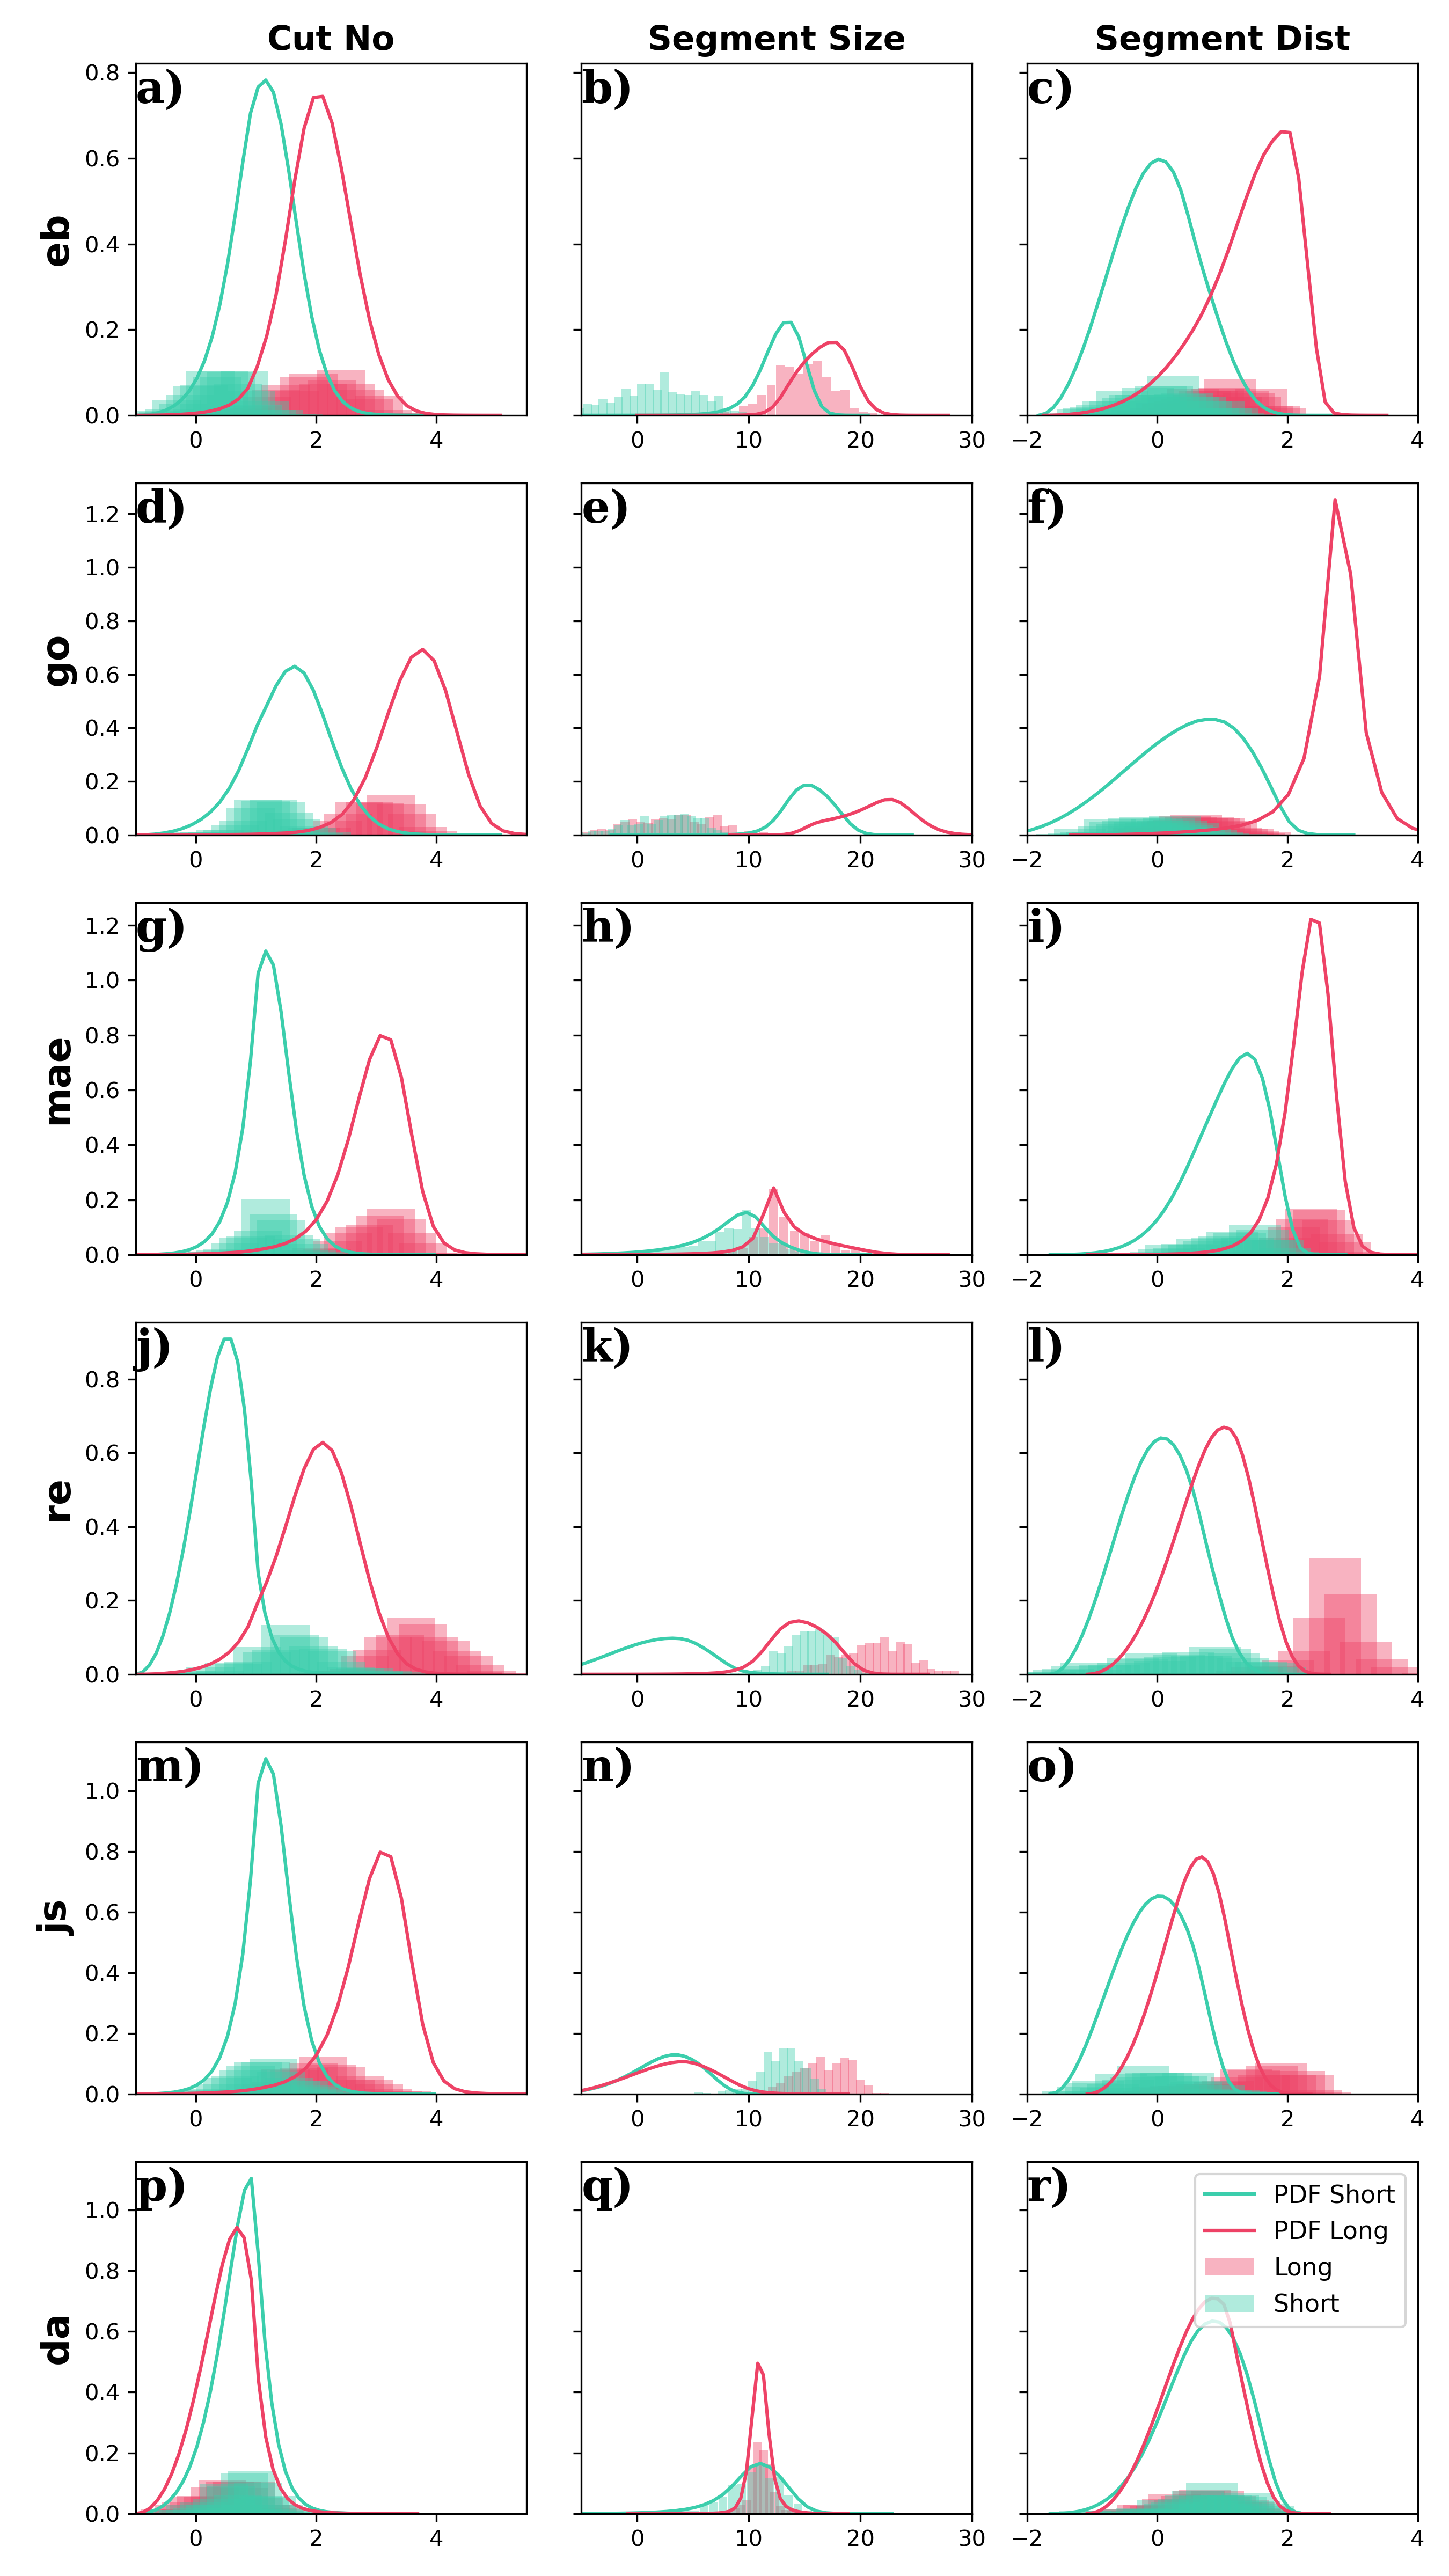
\includegraphics[width = \linewidth]{Thesis/plots/marginalDensities.png}
    \caption{PDFs and drawn probabilities for the corresponding cut no, segment size, and segment distances.}
    \label{fig:mpd}
\end{figure}
\clearpage

\section{Goodness of fit}
\label{appendix:gof}
First row (Plots \textbf{a} and \textbf{b}) shows the histograms of Monte-Carlo-generated deviance distribution from the fitted psychometric function. Short and long exposure times were analyzed separately. The vertical line shows the deviance of the observed data.

Second and third rows (Plots \textbf{c} and \textbf{d}) have three plots based on the deviance residuals, which are deviations from the fitted psychometric function. Short and long exposure time conditions were analyzed separately.

The first plot displays the psychometric function along with the data surrounding it to provide a general overview. 

The second plot shows the deviance residuals plotted against the stimulus level, with three lines representing polynomial functions of first, second, and third order fitted to the data points. This plot is useful in identifying whether the data systematically deviates from the psychometric function at different stimulus levels, which could indicate a poor fit between the psychometric function and the data. 

The third plot displays the deviance residuals against the block order, which helps in detecting any changes in performance over time. 

These analyses were performed separately for each participant and each predictor (cut no, segment size, and segment distance).

\clearpage
\subsection{Segment Size}
\subsubsection*{E.B.}
\begin{figure}[!hb]
    \begin{subfigure}{0.494\textwidth}
        \centering
        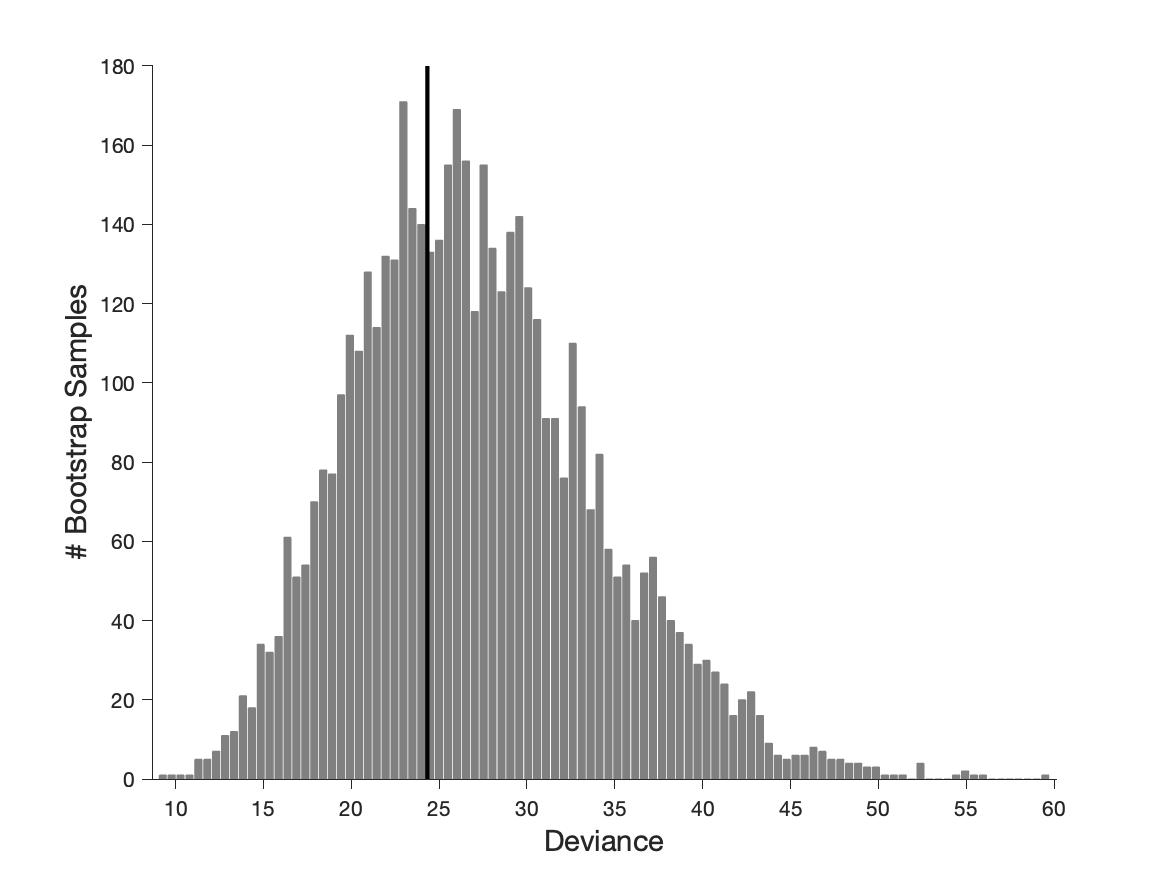
\includegraphics[width = \linewidth]{Thesis/plots/gof/segSize/segSize_eb_short_bootstrap.png}
        \caption{Monte-Carlo generated deviance histograms for short exposure time}
        \label{fig:da_gof_short_bootstrap}
    \end{subfigure}
    \hspace{0.01\textwidth}
    \begin{subfigure}{0.494\textwidth}
        \centering
        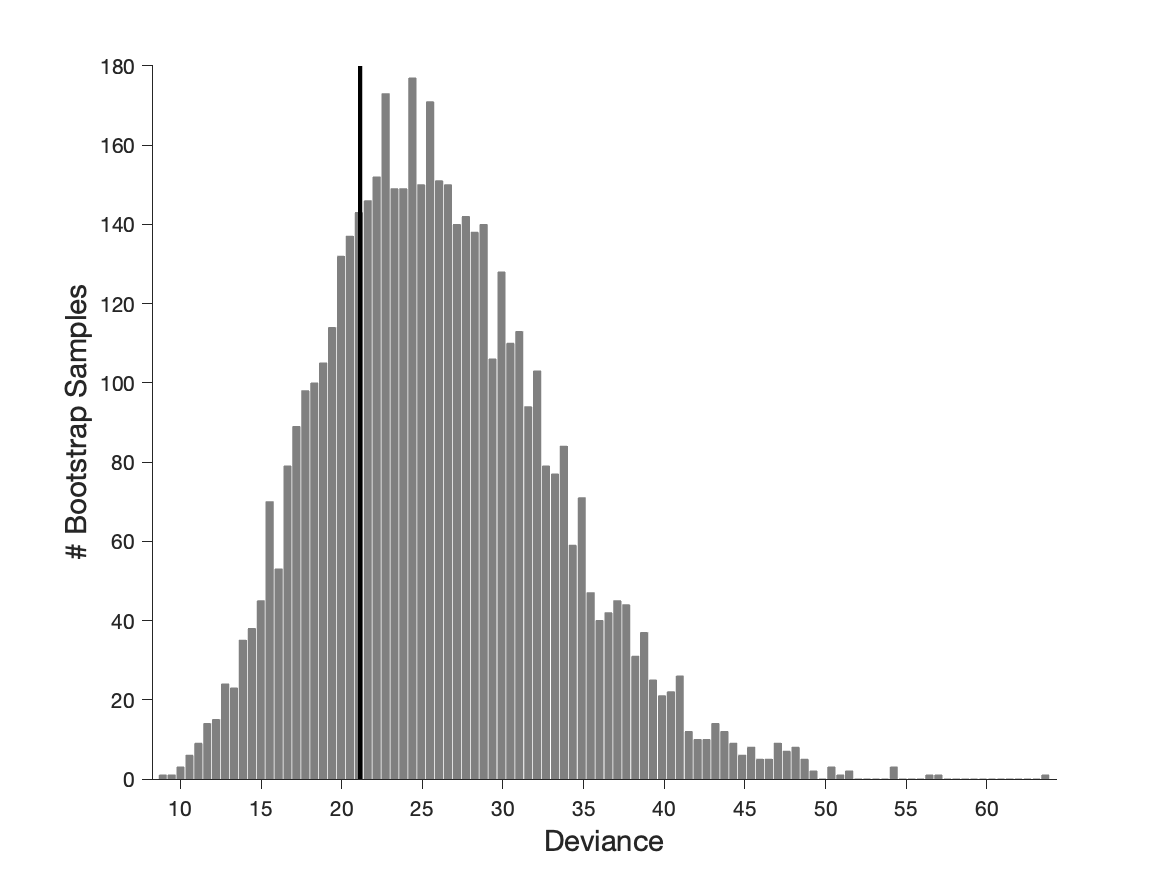
\includegraphics[width = \linewidth]{Thesis/plots/gof/segSize/segSize_eb_long_bootstrap.png}
        \caption{Monte-Carlo generated deviance histograms for long exposure time}
        \label{fig:da_gof_long_bootstrap}
    \end{subfigure}
    
    \begin{subfigure}{\textwidth}
        \centering
        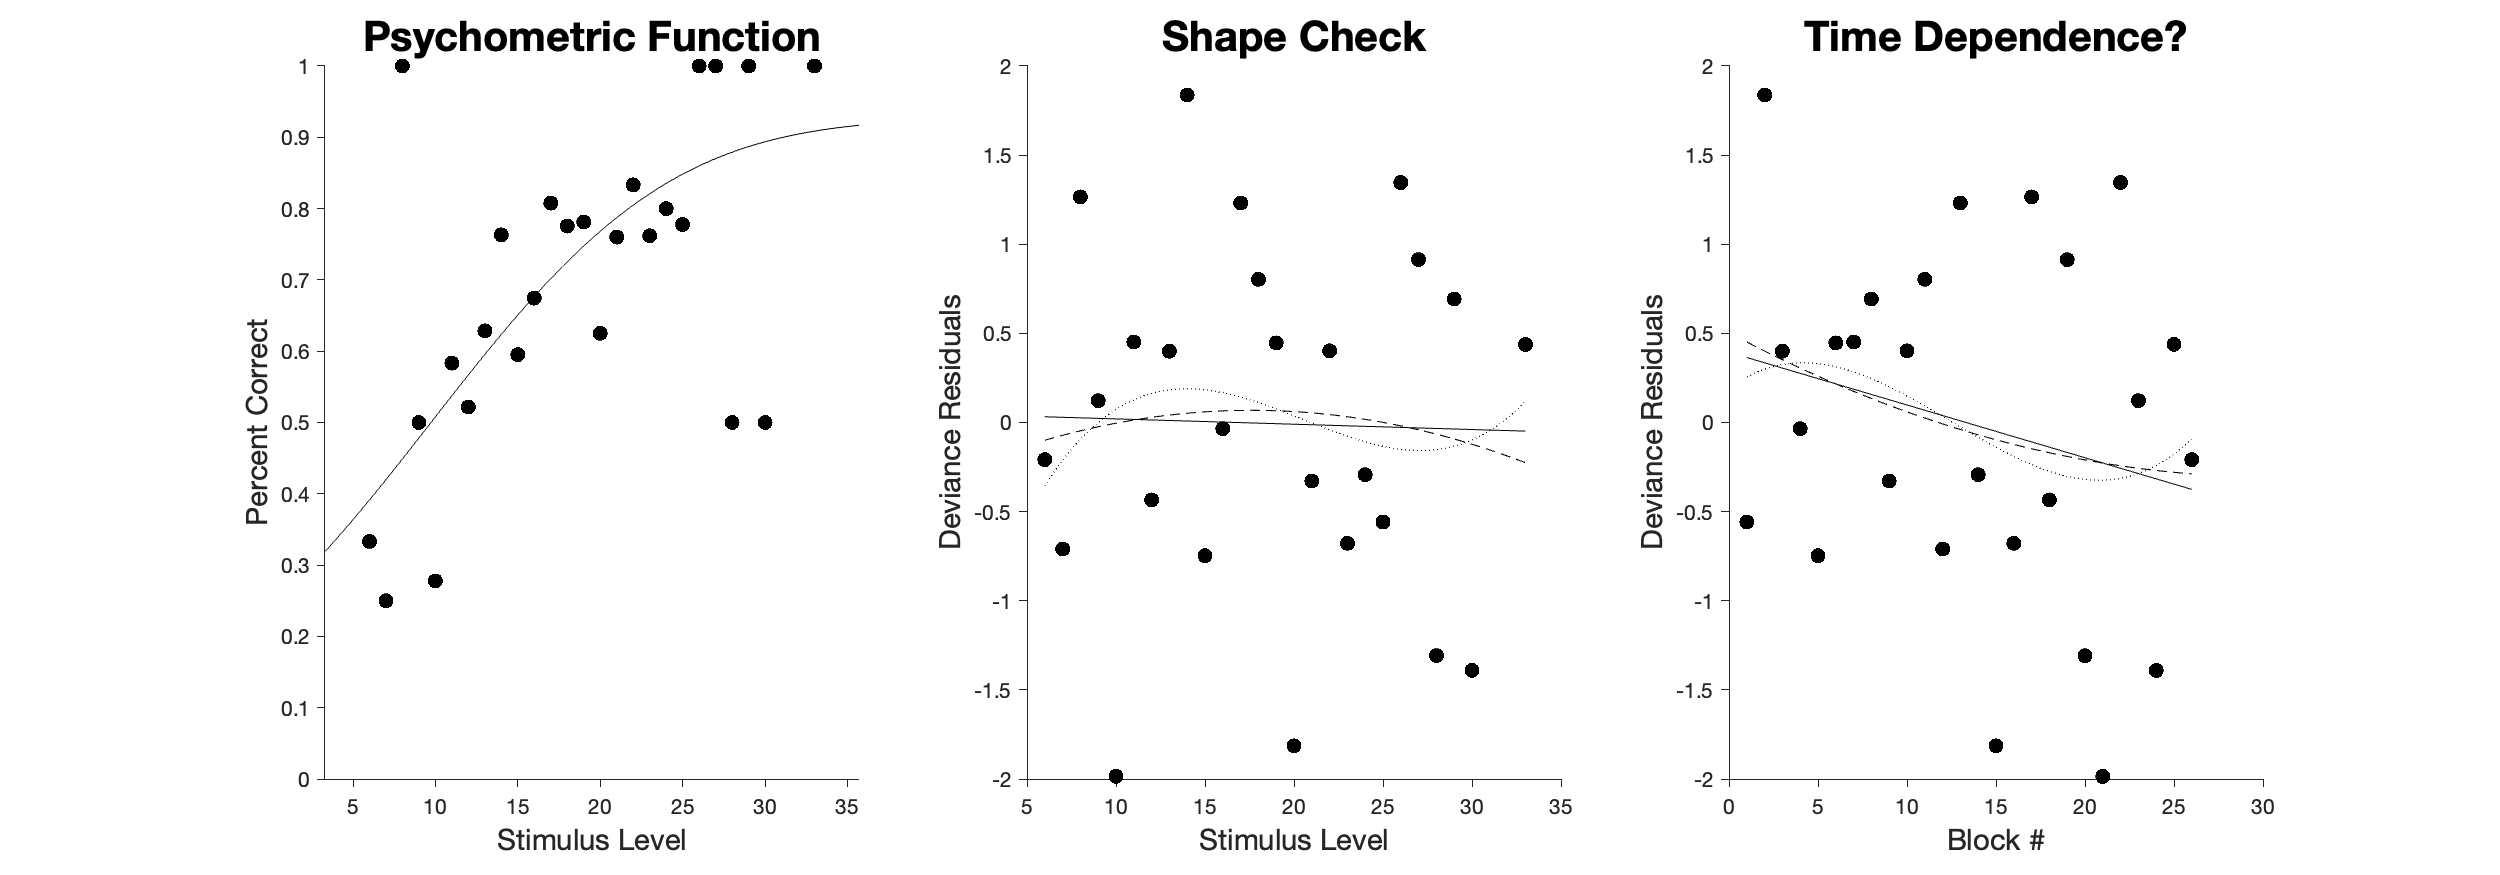
\includegraphics[width = \linewidth]{Thesis/plots/gof/segSize/segSize_eb_short_deviance.png}
        \caption{Deviance residuals for short exposure time}
    \end{subfigure}
    
    \begin{subfigure}{\textwidth}
        \centering
        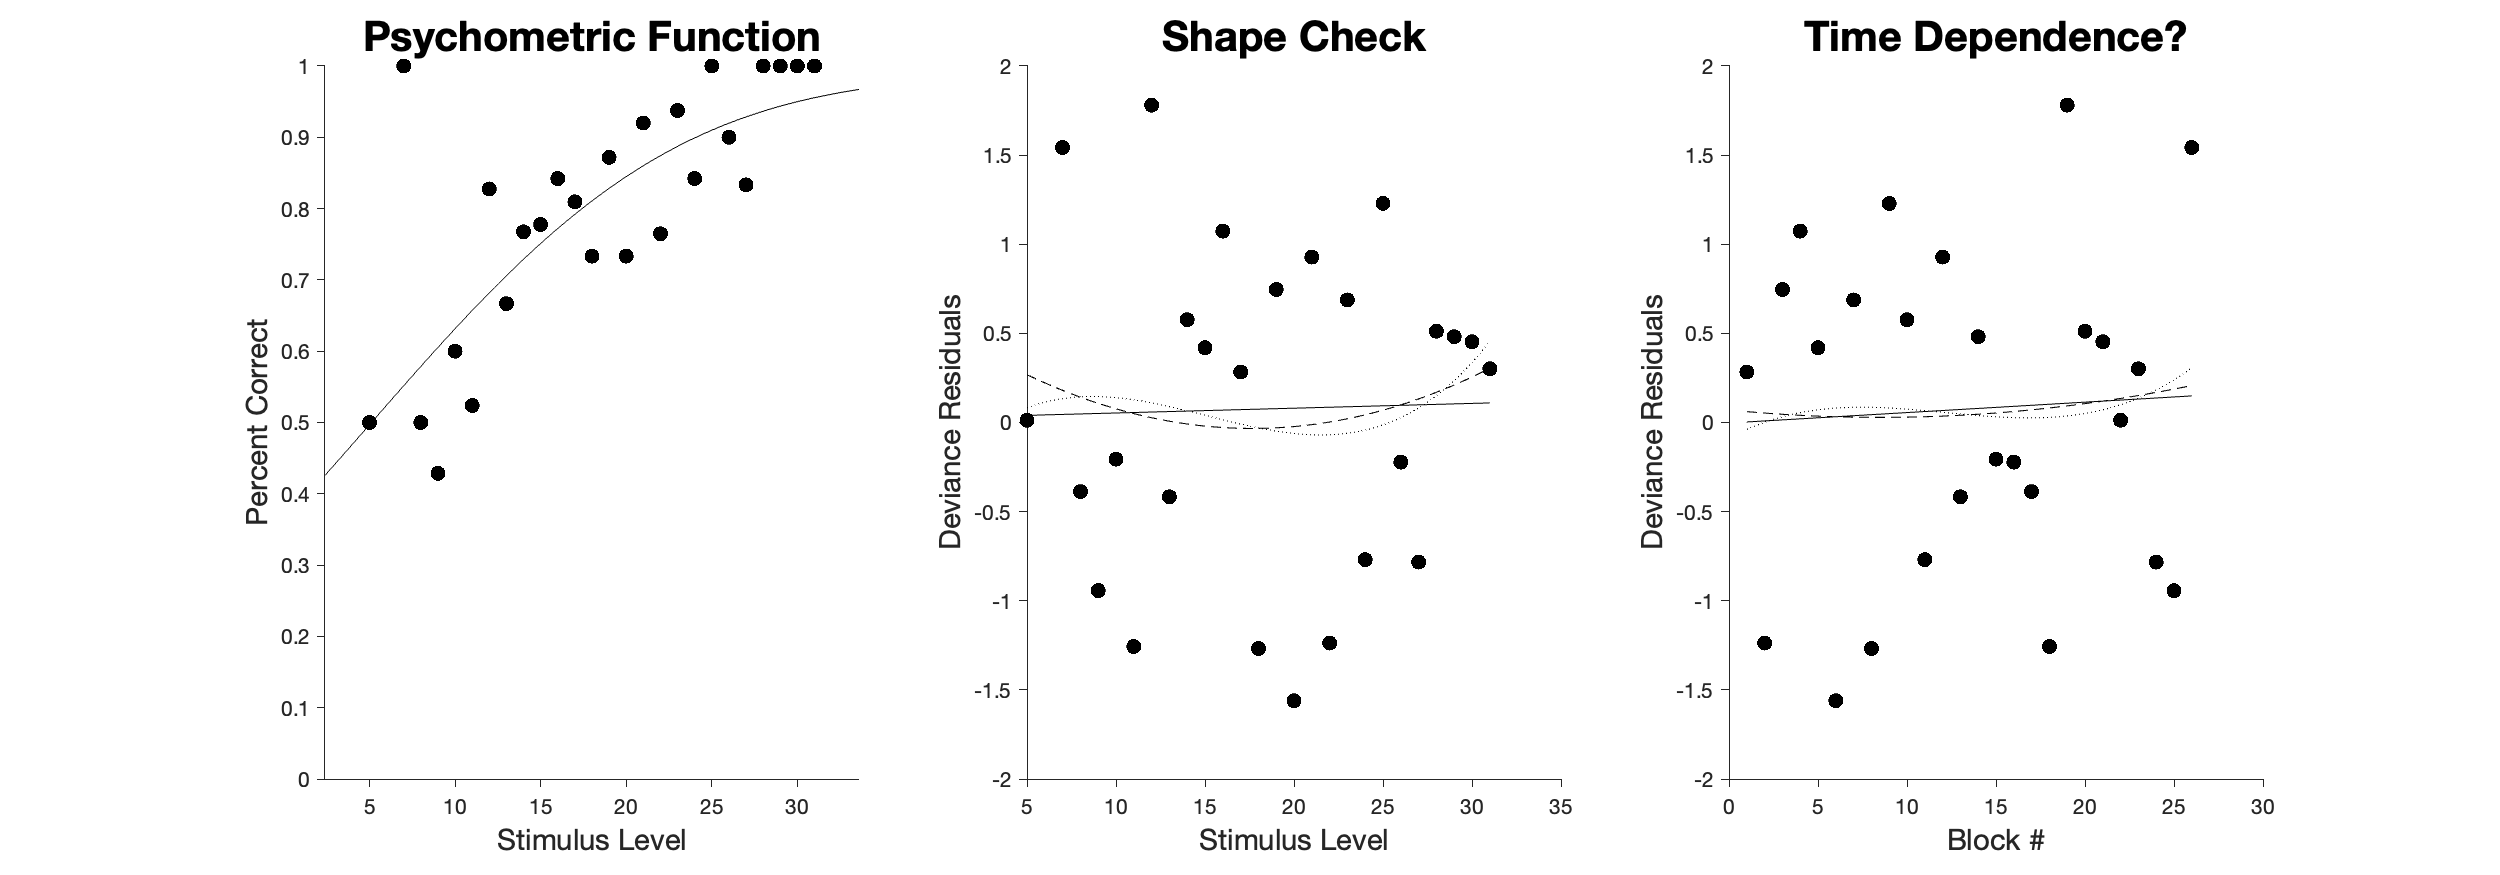
\includegraphics[width = \linewidth]{Thesis/plots/gof/segSize/segSize_eb_long_deviance.png}
        \caption{Deviance residuals for long exposure time}
    \end{subfigure}
\end{figure}

\clearpage

\subsubsection*{G.O.}
\begin{figure}[!hb]
    \begin{subfigure}{0.494\textwidth}
        \centering
        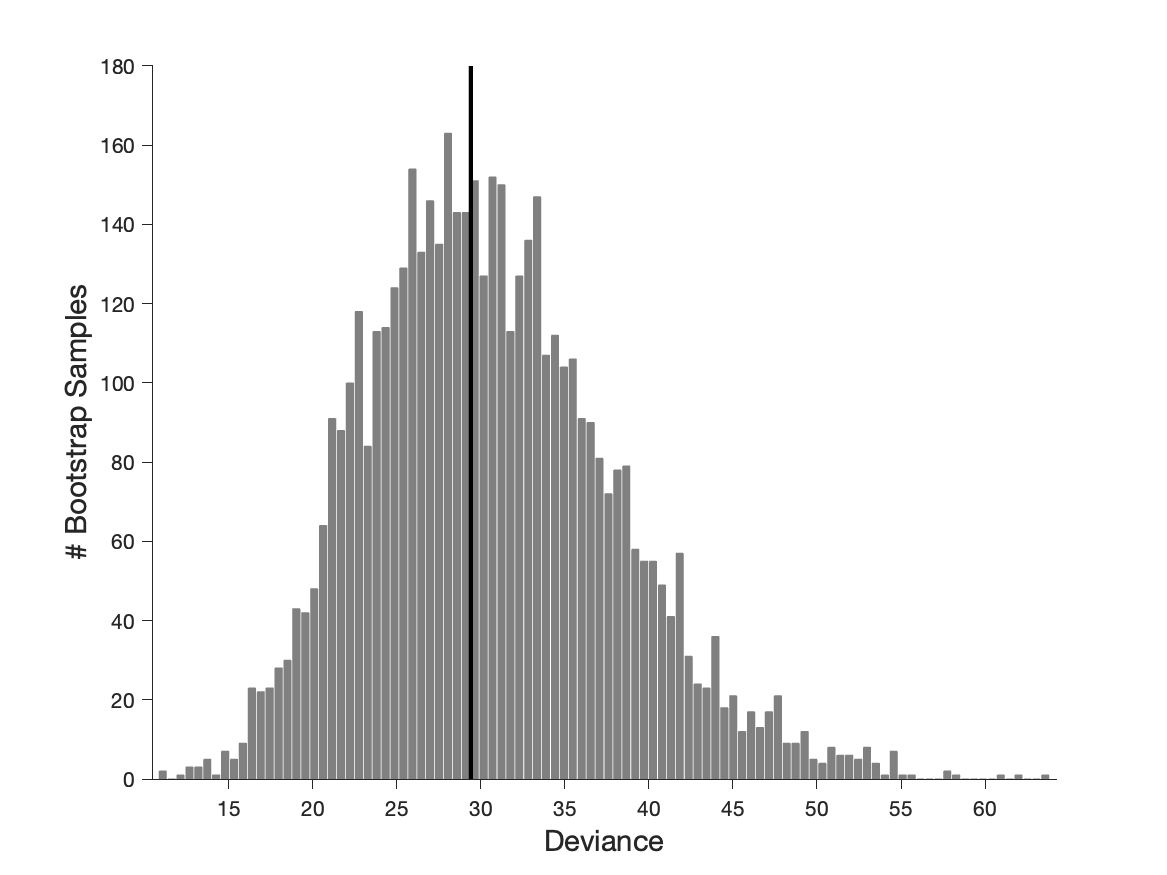
\includegraphics[width = \linewidth]{Thesis/plots/gof/segSize/segSize_go_short_bootstrap.png}
        \caption{Monte-Carlo generated deviance histograms for short exposure time}
        \label{fig:da_gof_short_bootstrap}
    \end{subfigure}
    \hspace{0.01\textwidth}
    \begin{subfigure}{0.494\textwidth}
        \centering
        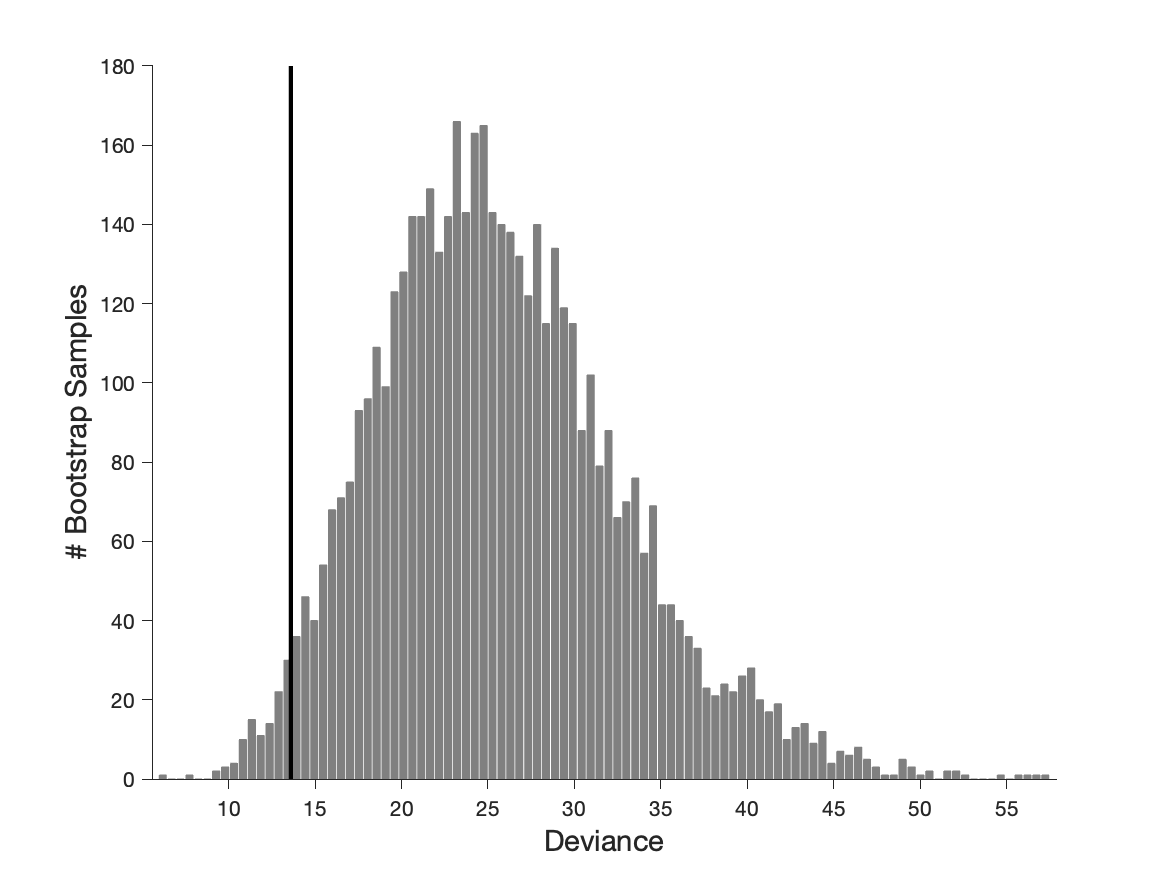
\includegraphics[width = \linewidth]{Thesis/plots/gof/segSize/segSize_go_long_bootstrap.png}
        \caption{Monte-Carlo generated deviance histograms for long exposure time}
        \label{fig:da_gof_long_bootstrap}
    \end{subfigure}
    
    \begin{subfigure}{\textwidth}
        \centering
        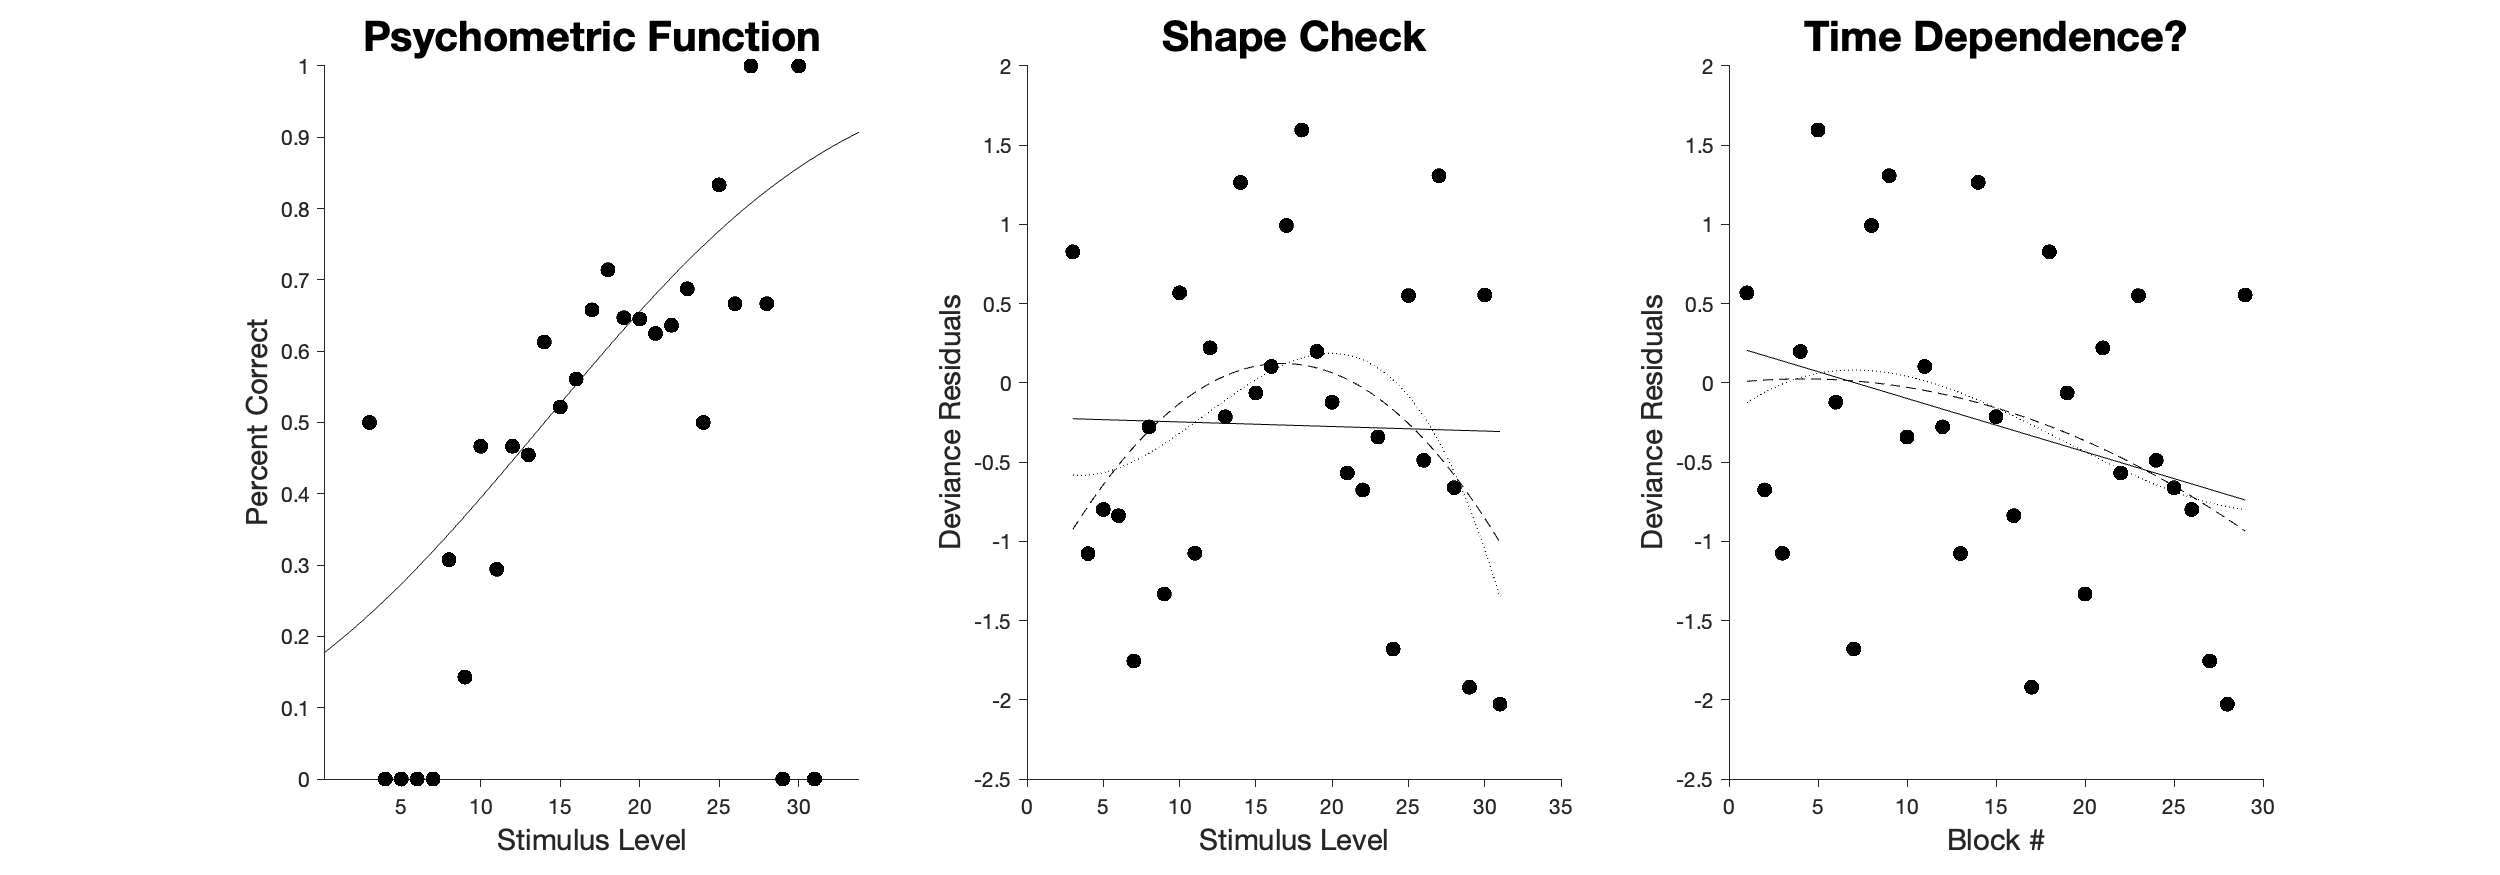
\includegraphics[width = \linewidth]{Thesis/plots/gof/segSize/segSize_go_short_deviance.png}
        \caption{Deviance residuals for short exposure time}
    \end{subfigure}
    
    \begin{subfigure}{\textwidth}
        \centering
        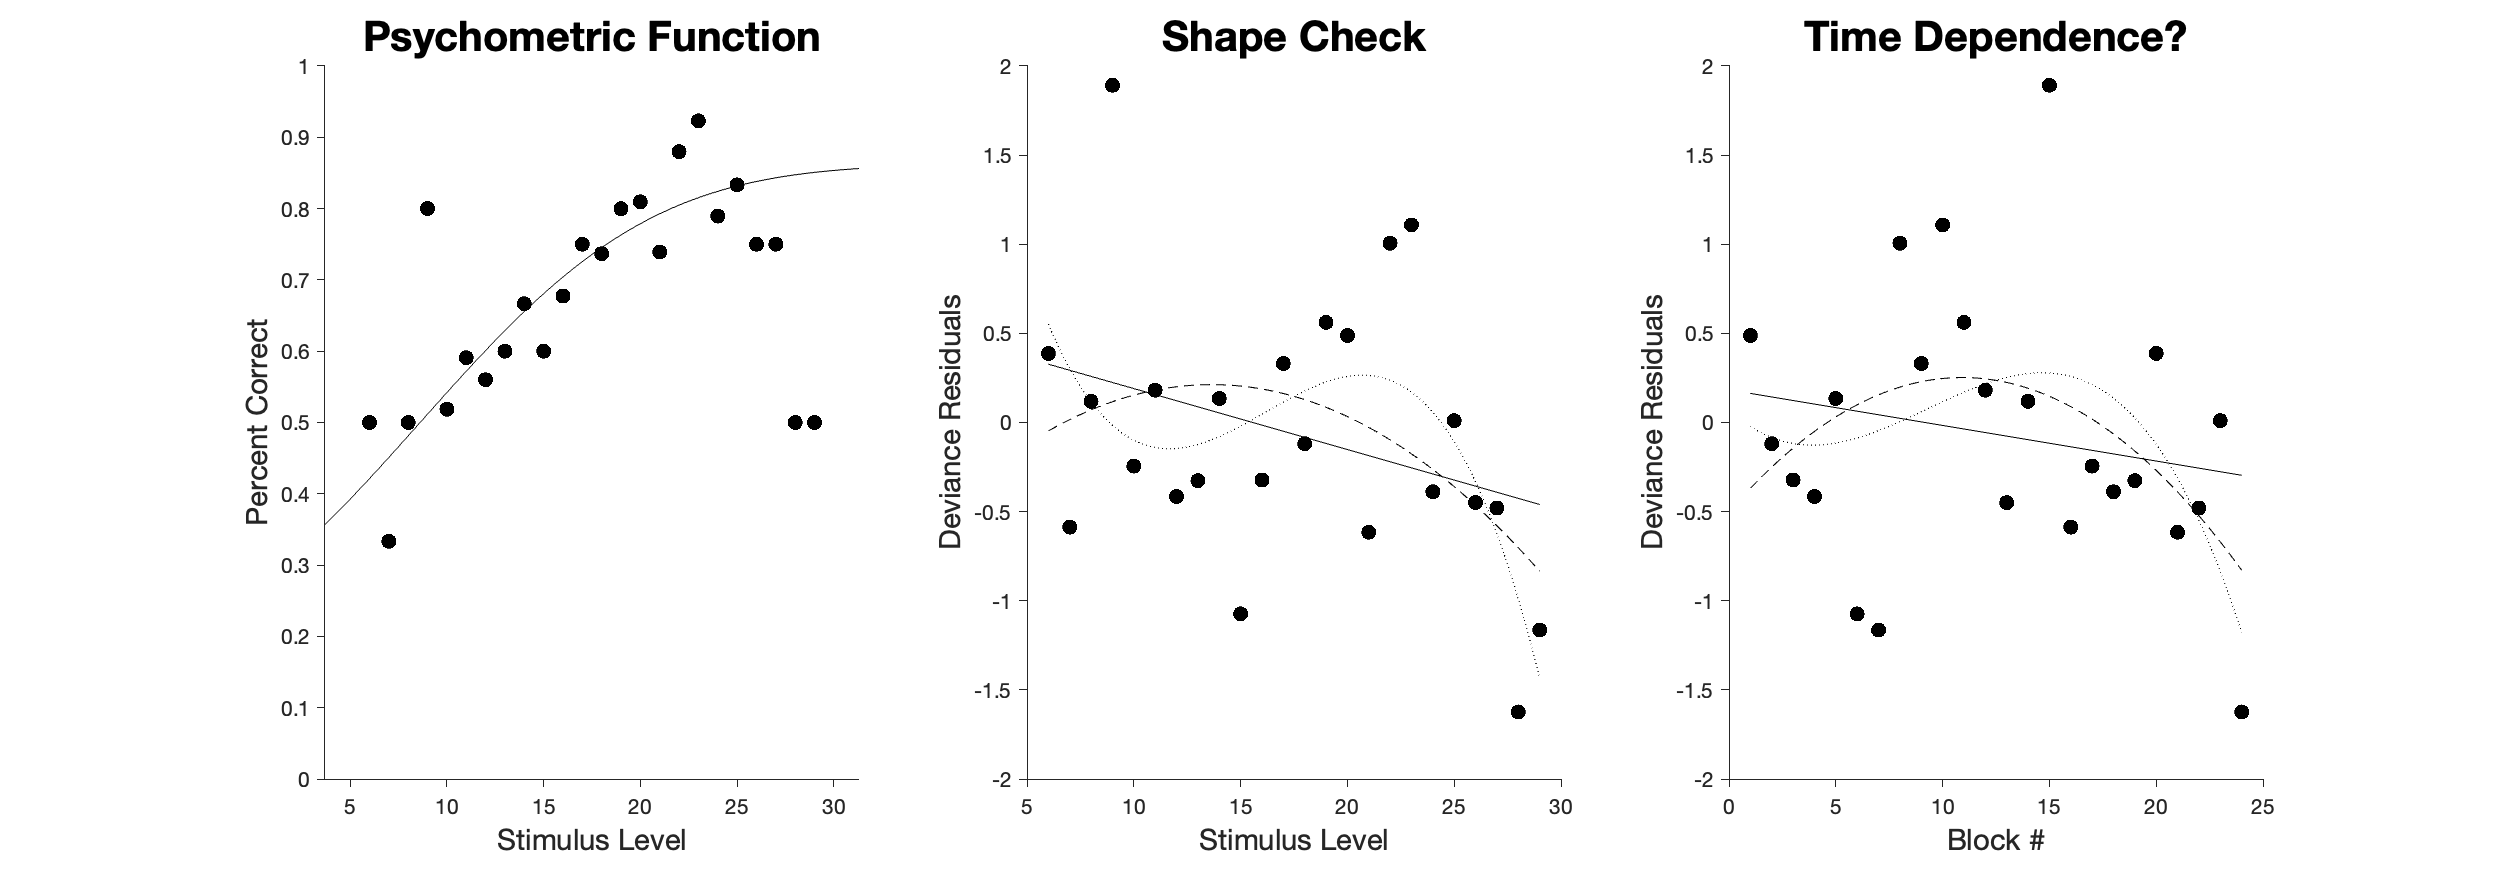
\includegraphics[width = \linewidth]{Thesis/plots/gof/segSize/segSize_go_long_deviance.png}
        \caption{Deviance residuals for long exposure time}
    \end{subfigure}
    
\end{figure}
\clearpage

\subsubsection*{M.A.E.}
\begin{figure}[!hb]
    \begin{subfigure}{0.494\textwidth}
        \centering
        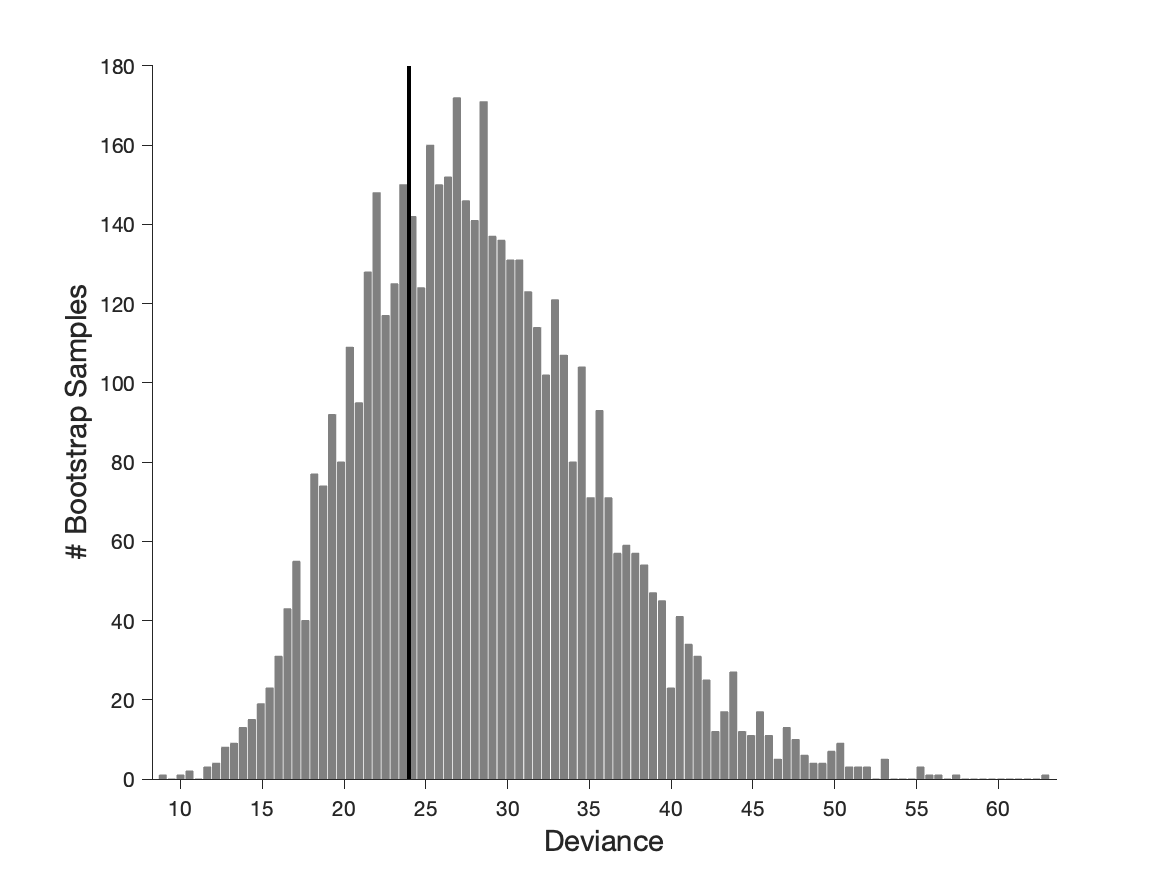
\includegraphics[width = \linewidth]{Thesis/plots/gof/segSize/segSize_mae_short_bootstrap.png}
        \caption{Monte-Carlo generated deviance histograms for short exposure time}
        \label{fig:da_gof_short_bootstrap}
    \end{subfigure}
    \hspace{0.01\textwidth}
    \begin{subfigure}{0.494\textwidth}
        \centering
        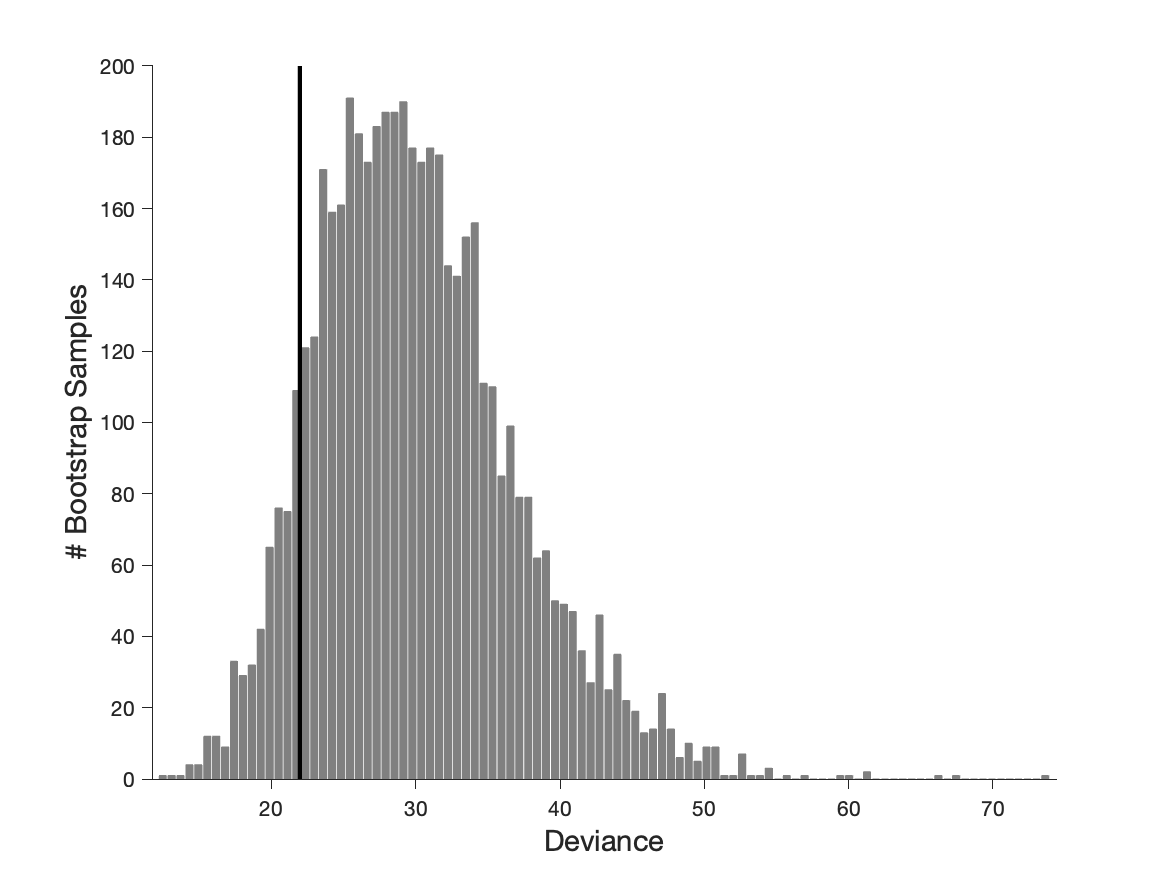
\includegraphics[width = \linewidth]{Thesis/plots/gof/segSize/segSize_mae_long_bootstrap.png}
        \caption{Monte-Carlo generated deviance histograms for long exposure time}
        \label{fig:da_gof_long_bootstrap}
    \end{subfigure}
    
    \begin{subfigure}{\textwidth}
        \centering
        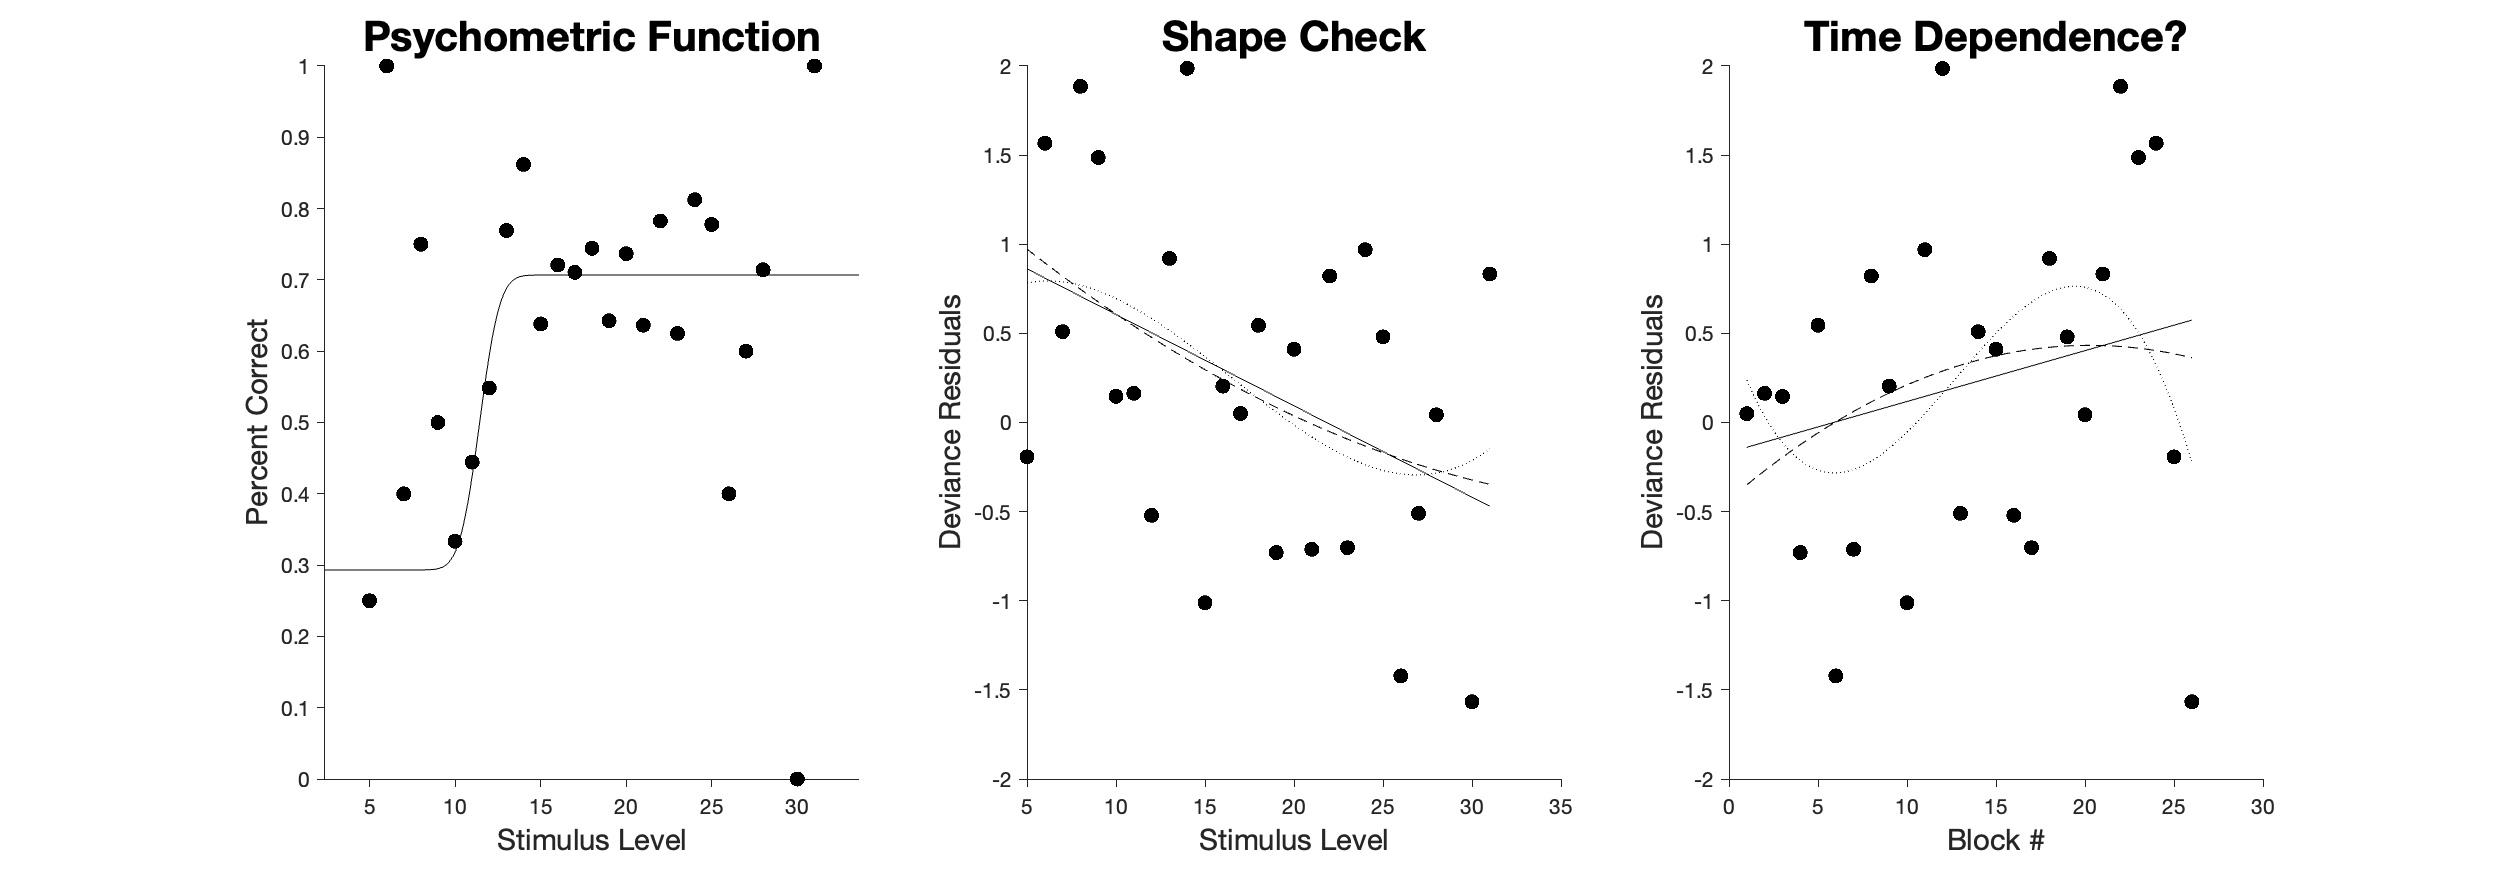
\includegraphics[width = \linewidth]{Thesis/plots/gof/segSize/segSize_mae_short_deviance.png}
        \caption{Deviance residuals for short exposure time}
    \end{subfigure}
    \begin{subfigure}{\textwidth}
        \centering
        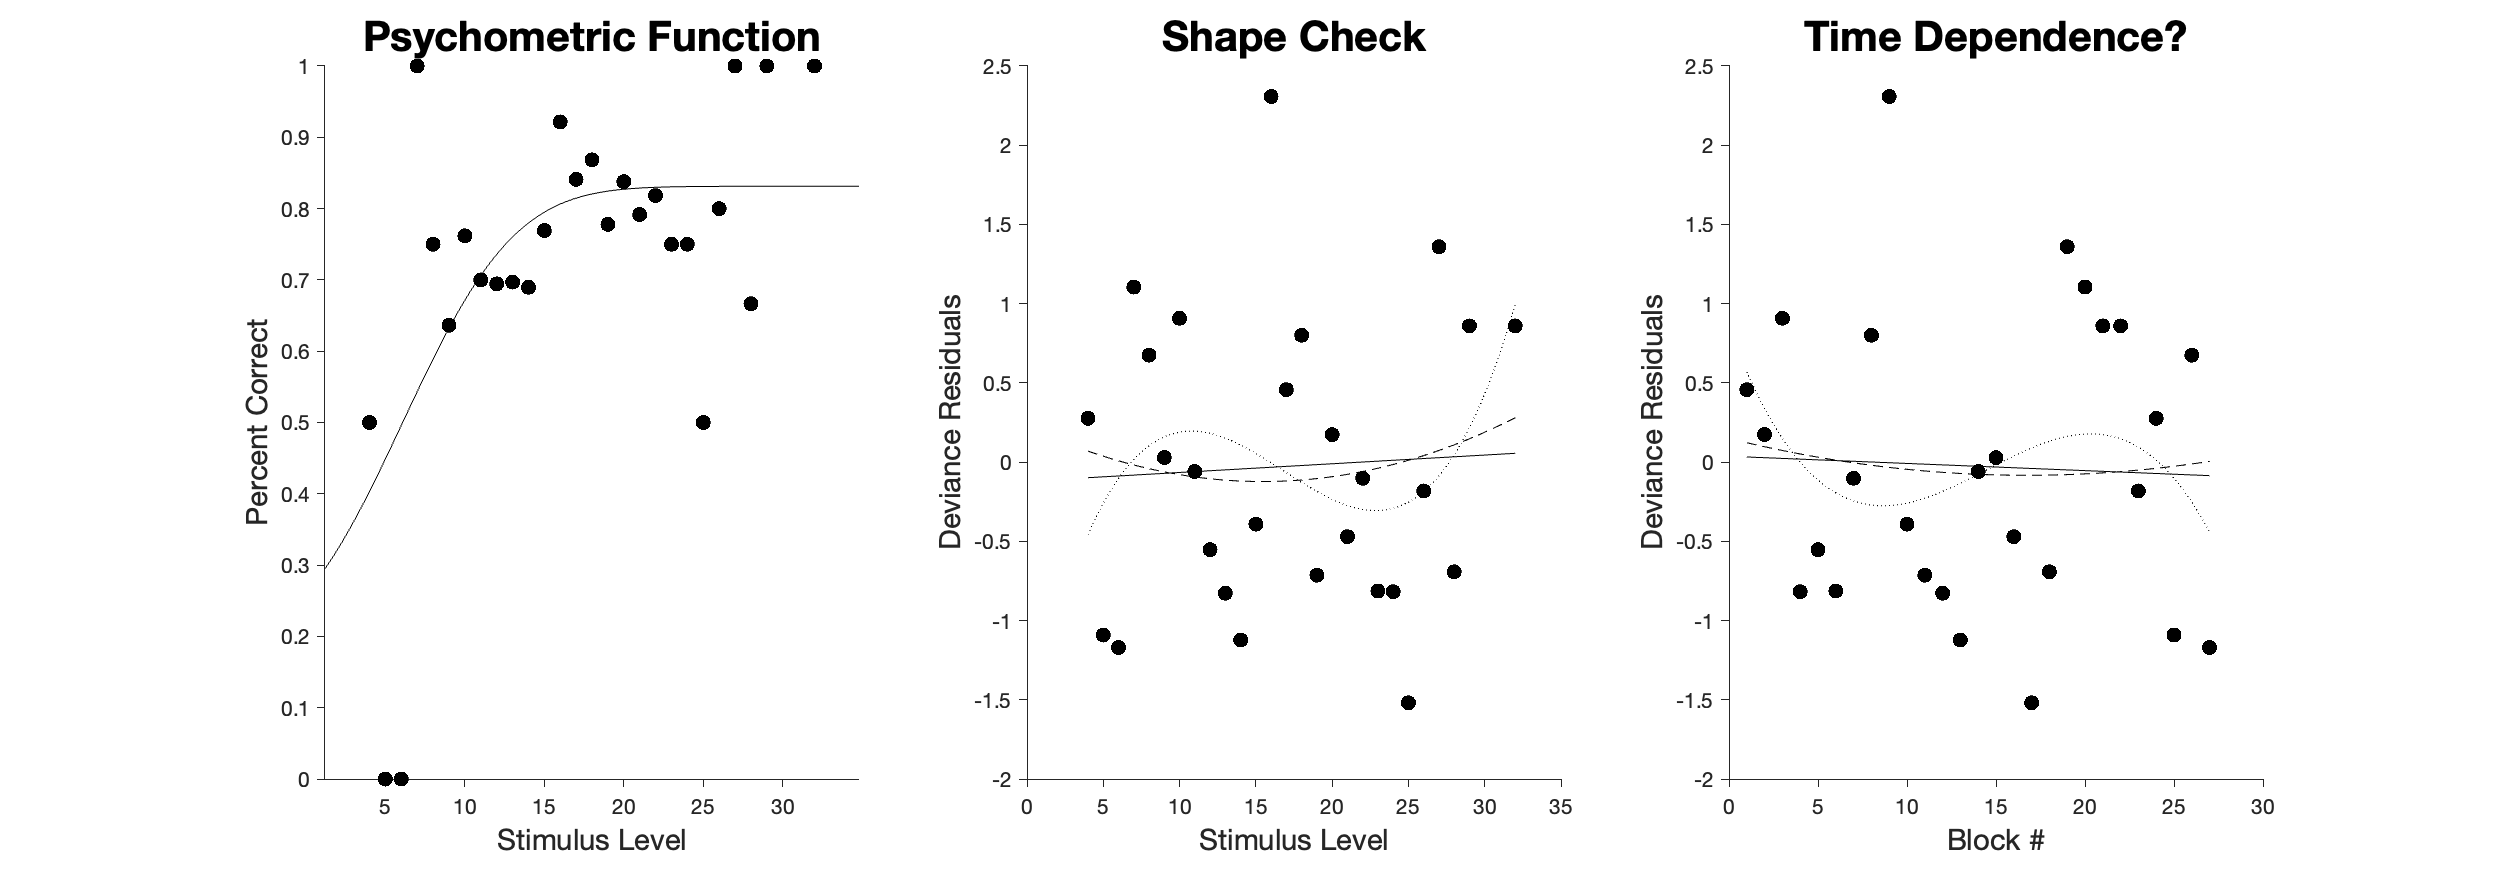
\includegraphics[width = \linewidth]{Thesis/plots/gof/segSize/segSize_mae_long_deviance.png}
        \caption{Deviance residuals for long exposure time}
    \end{subfigure}
\end{figure}

\clearpage

\subsubsection*{R.E.}
\begin{figure}[!hb]
    \begin{subfigure}{0.494\textwidth}
        \centering
        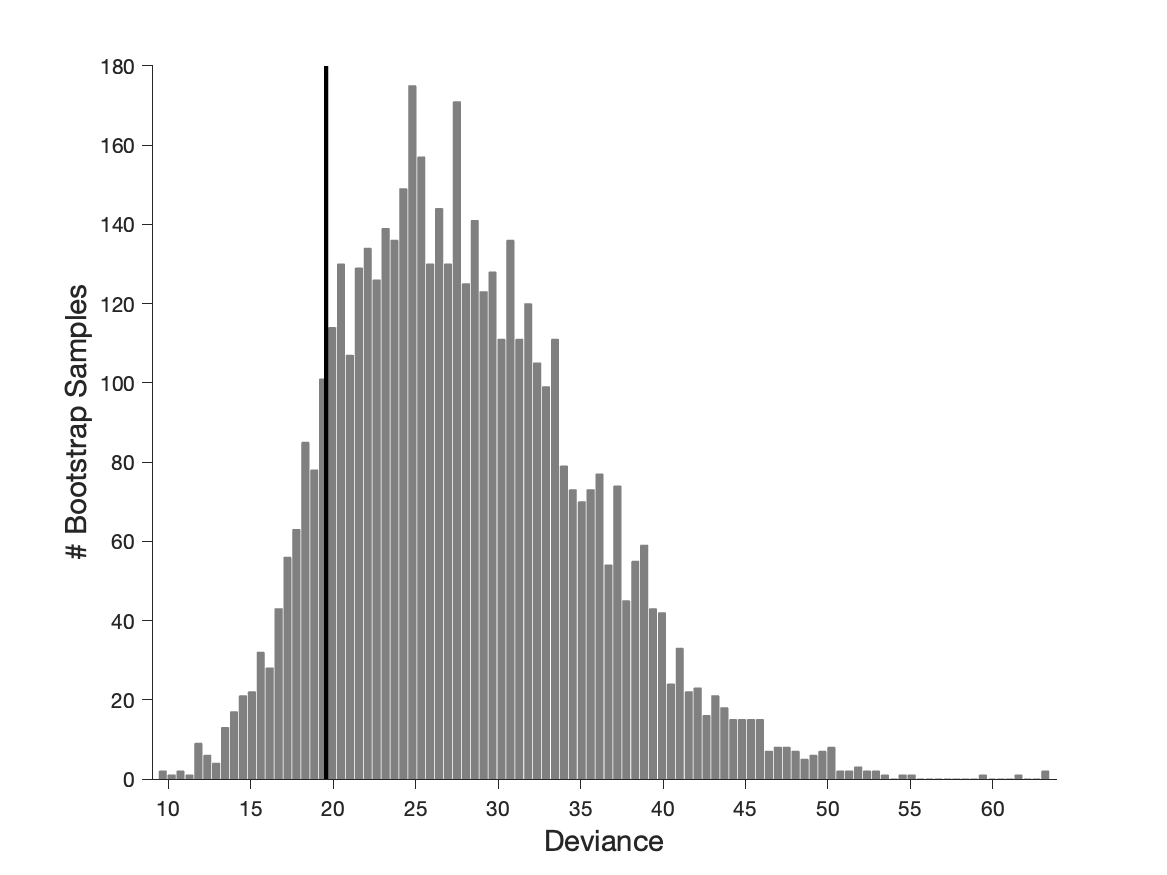
\includegraphics[width = \linewidth]{Thesis/plots/gof/segSize/segSize_re_short_bootstrap.png}
        \caption{Monte-Carlo generated deviance histograms for short exposure time}
        \label{fig:da_gof_short_bootstrap}
    \end{subfigure}
    \hspace{0.01\textwidth}
    \begin{subfigure}{0.494\textwidth}
        \centering
        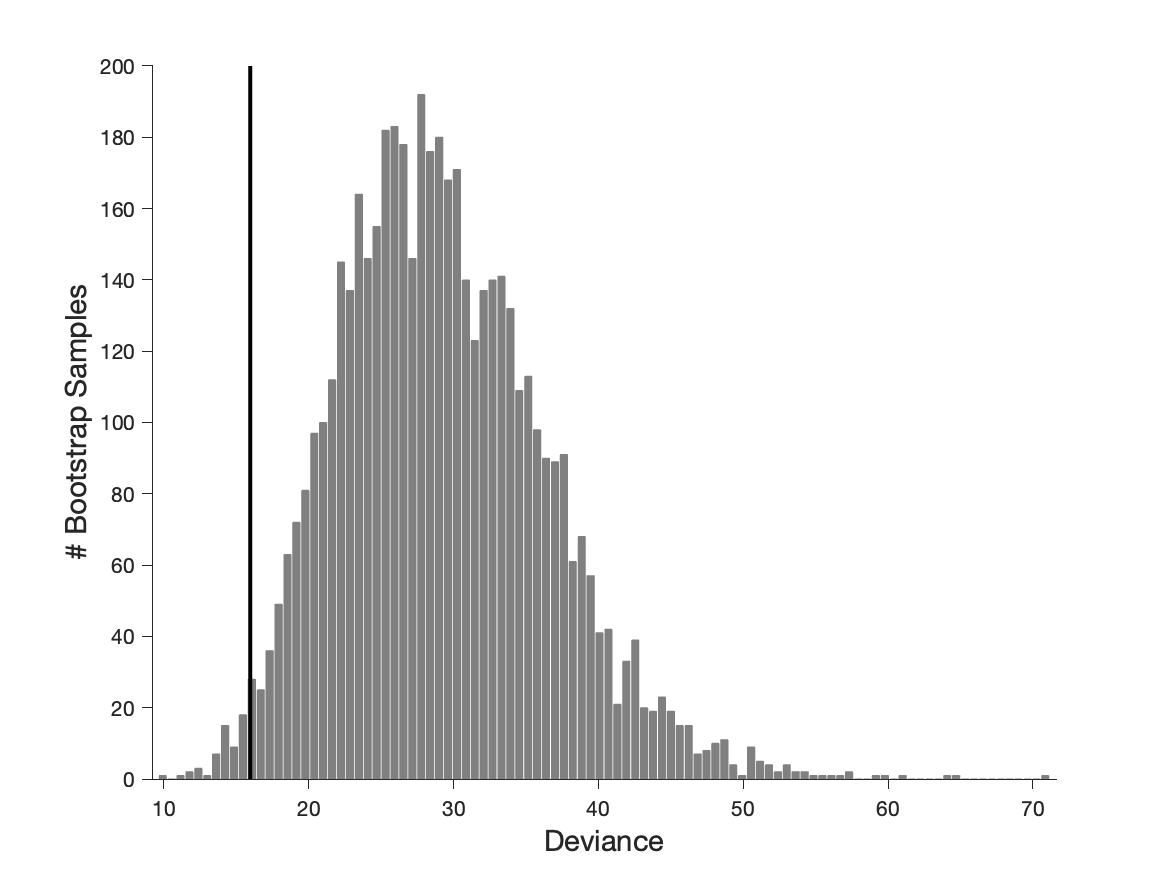
\includegraphics[width = \linewidth]{Thesis/plots/gof/segSize/segSize_re_long_bootstrap.png}
        \caption{Monte-Carlo generated deviance histograms for long exposure time}
        \label{fig:da_gof_long_bootstrap}
    \end{subfigure}
    
    \begin{subfigure}{\textwidth}
        \centering
        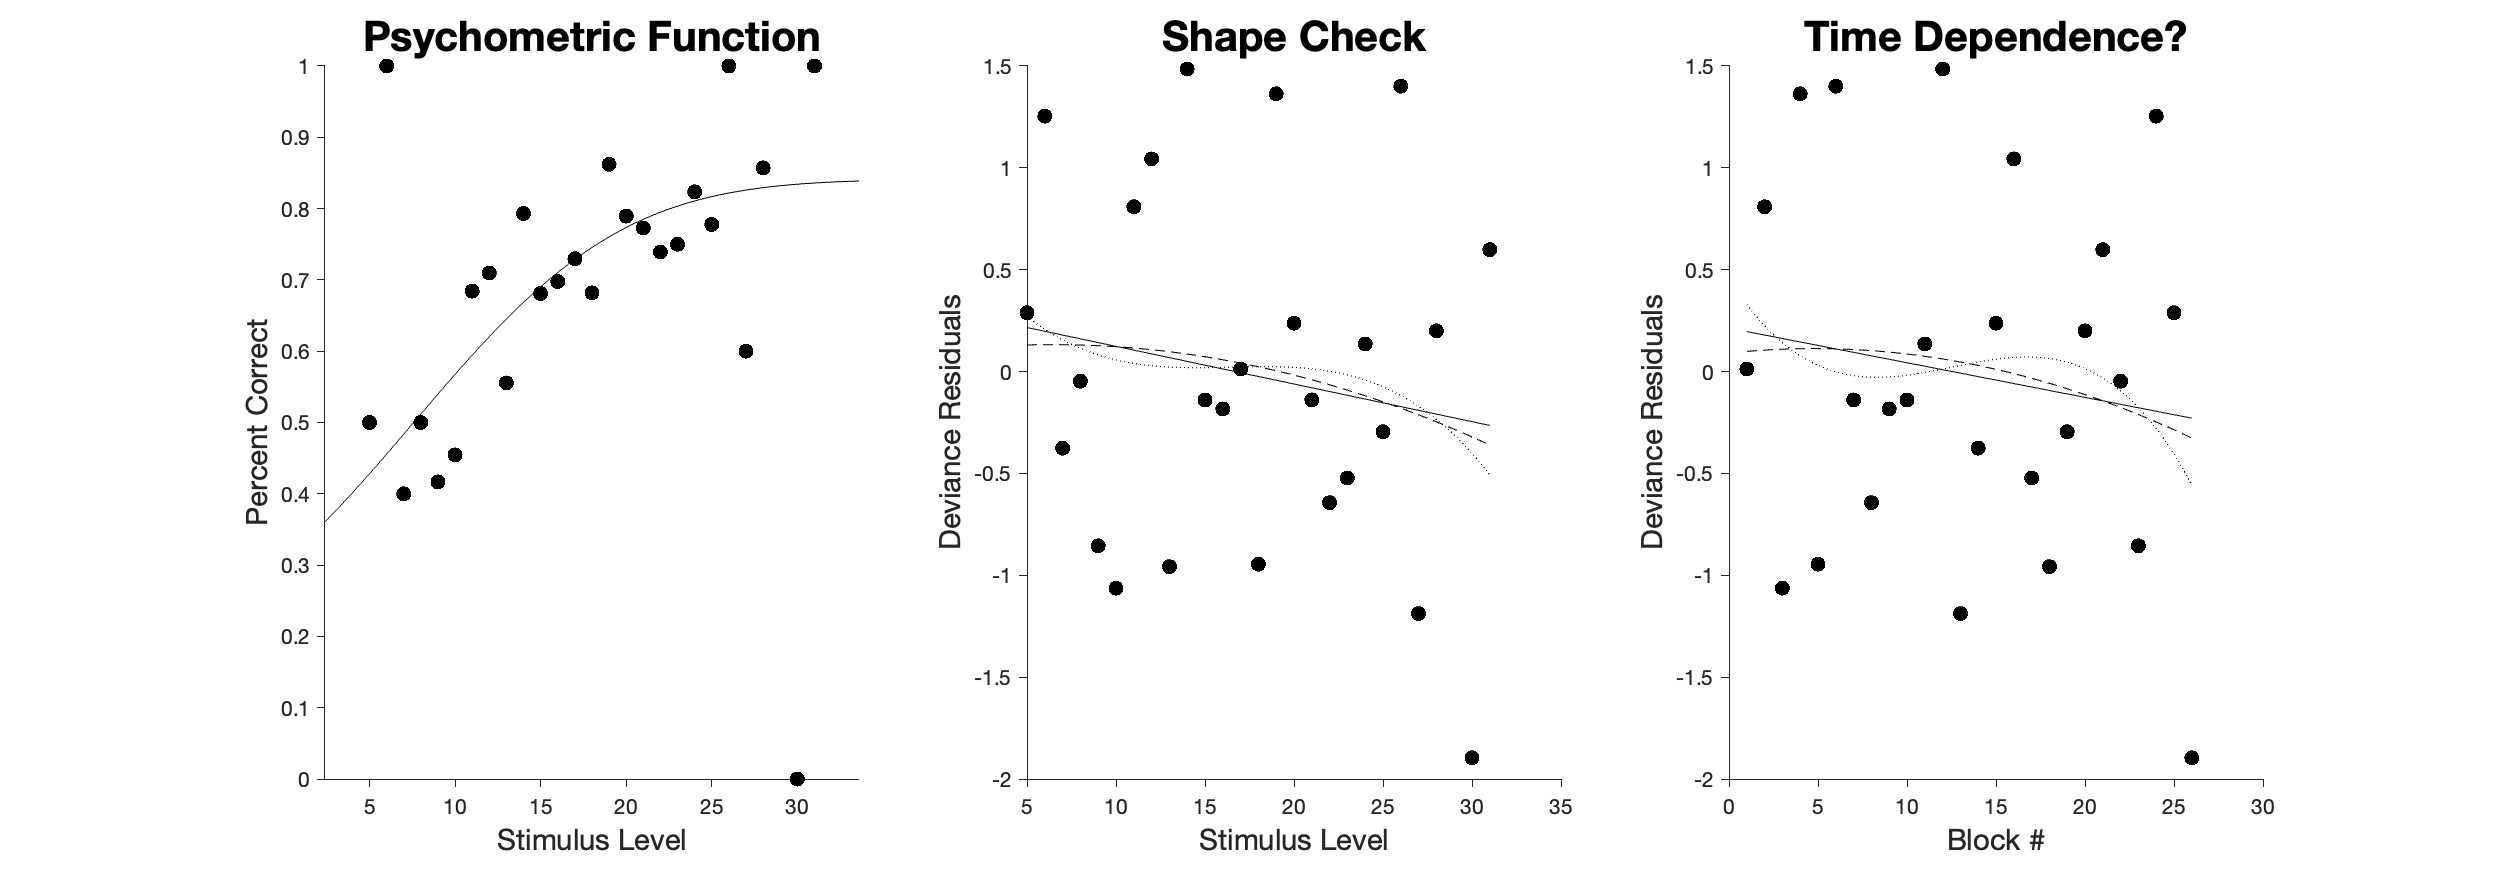
\includegraphics[width = \linewidth]{Thesis/plots/gof/segSize/segSize_re_short_deviance.png}
        \caption{Deviance residuals for short exposure time}
    \end{subfigure}
    
    \begin{subfigure}{\textwidth}
        \centering
        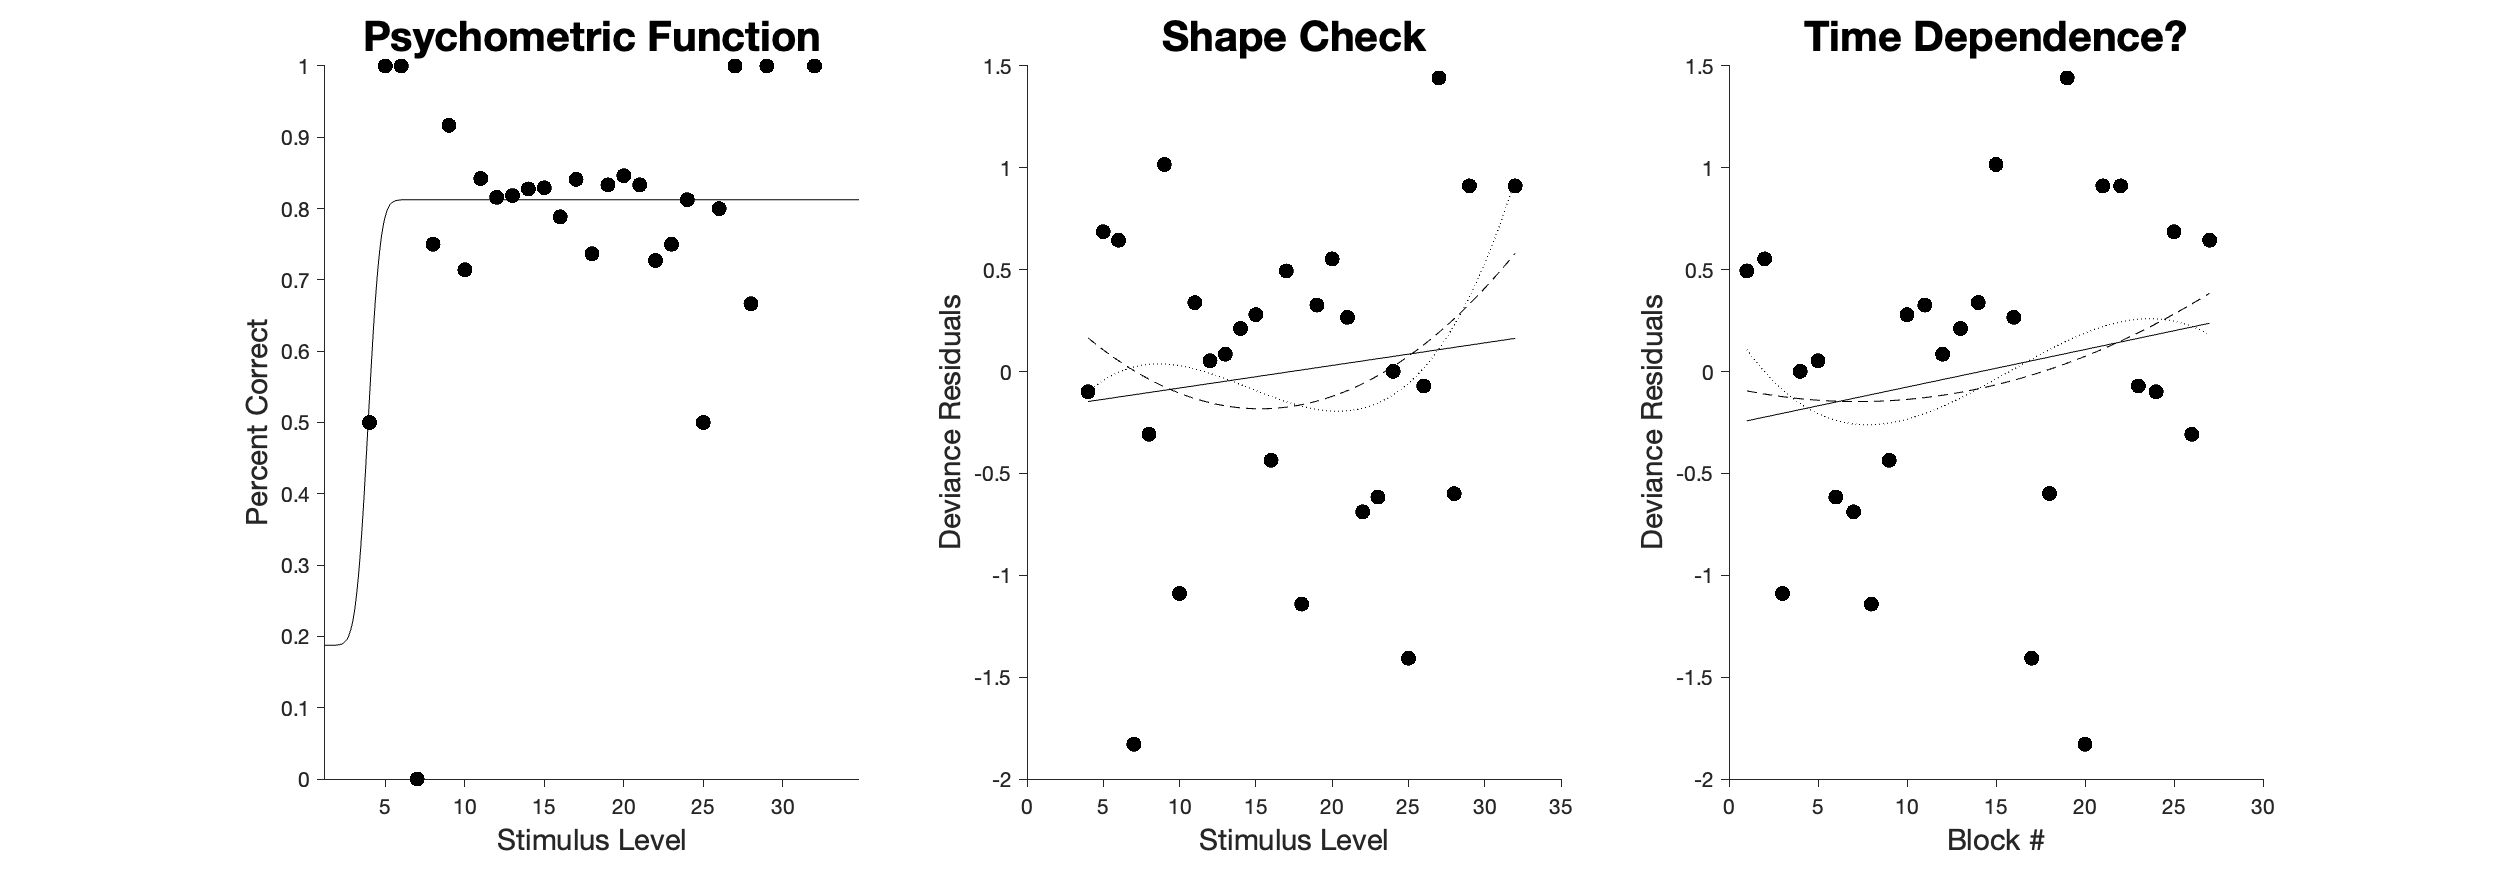
\includegraphics[width = \linewidth]{Thesis/plots/gof/segSize/segSize_re_long_deviance.png}
        \caption{Deviance residuals for long exposure time}
    \end{subfigure}
\end{figure}

\clearpage

\subsubsection*{D.A.}
\begin{figure}[!hb]
    \begin{subfigure}{0.494\textwidth}
        \centering
        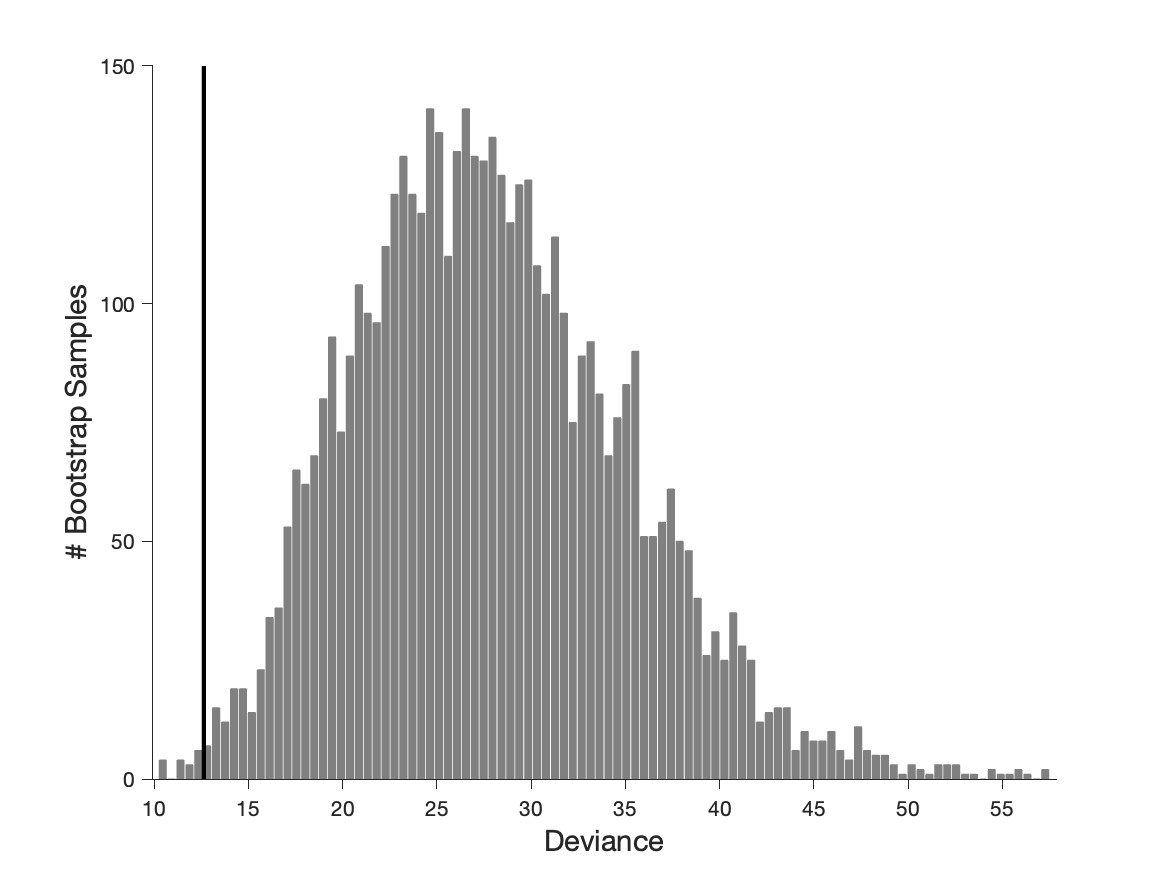
\includegraphics[width = \linewidth]{Thesis/plots/gof/segSize/segSize_da_short_bootstrap.png}
        \caption{Monte-Carlo generated deviance histograms for short exposure time}
        \label{fig:da_gof_short_bootstrap}
    \end{subfigure}
    \hspace{0.01\textwidth}
    \begin{subfigure}{0.494\textwidth}
        \centering
        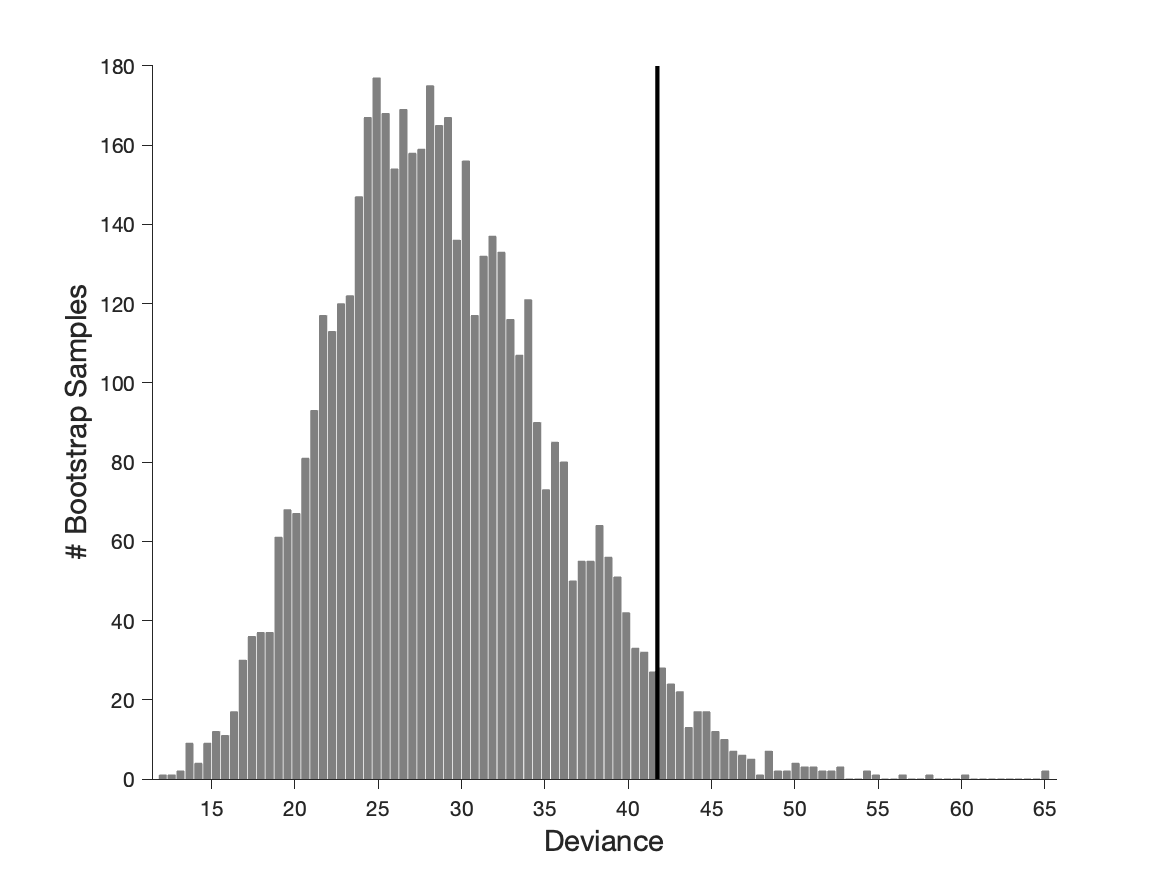
\includegraphics[width = \linewidth]{Thesis/plots/gof/segSize/segSize_da_long_bootstrap.png}
        \caption{Monte-Carlo generated deviance histograms for long exposure time}
        \label{fig:da_gof_long_bootstrap}
    \end{subfigure}
    
    \begin{subfigure}{\textwidth}
        \centering
        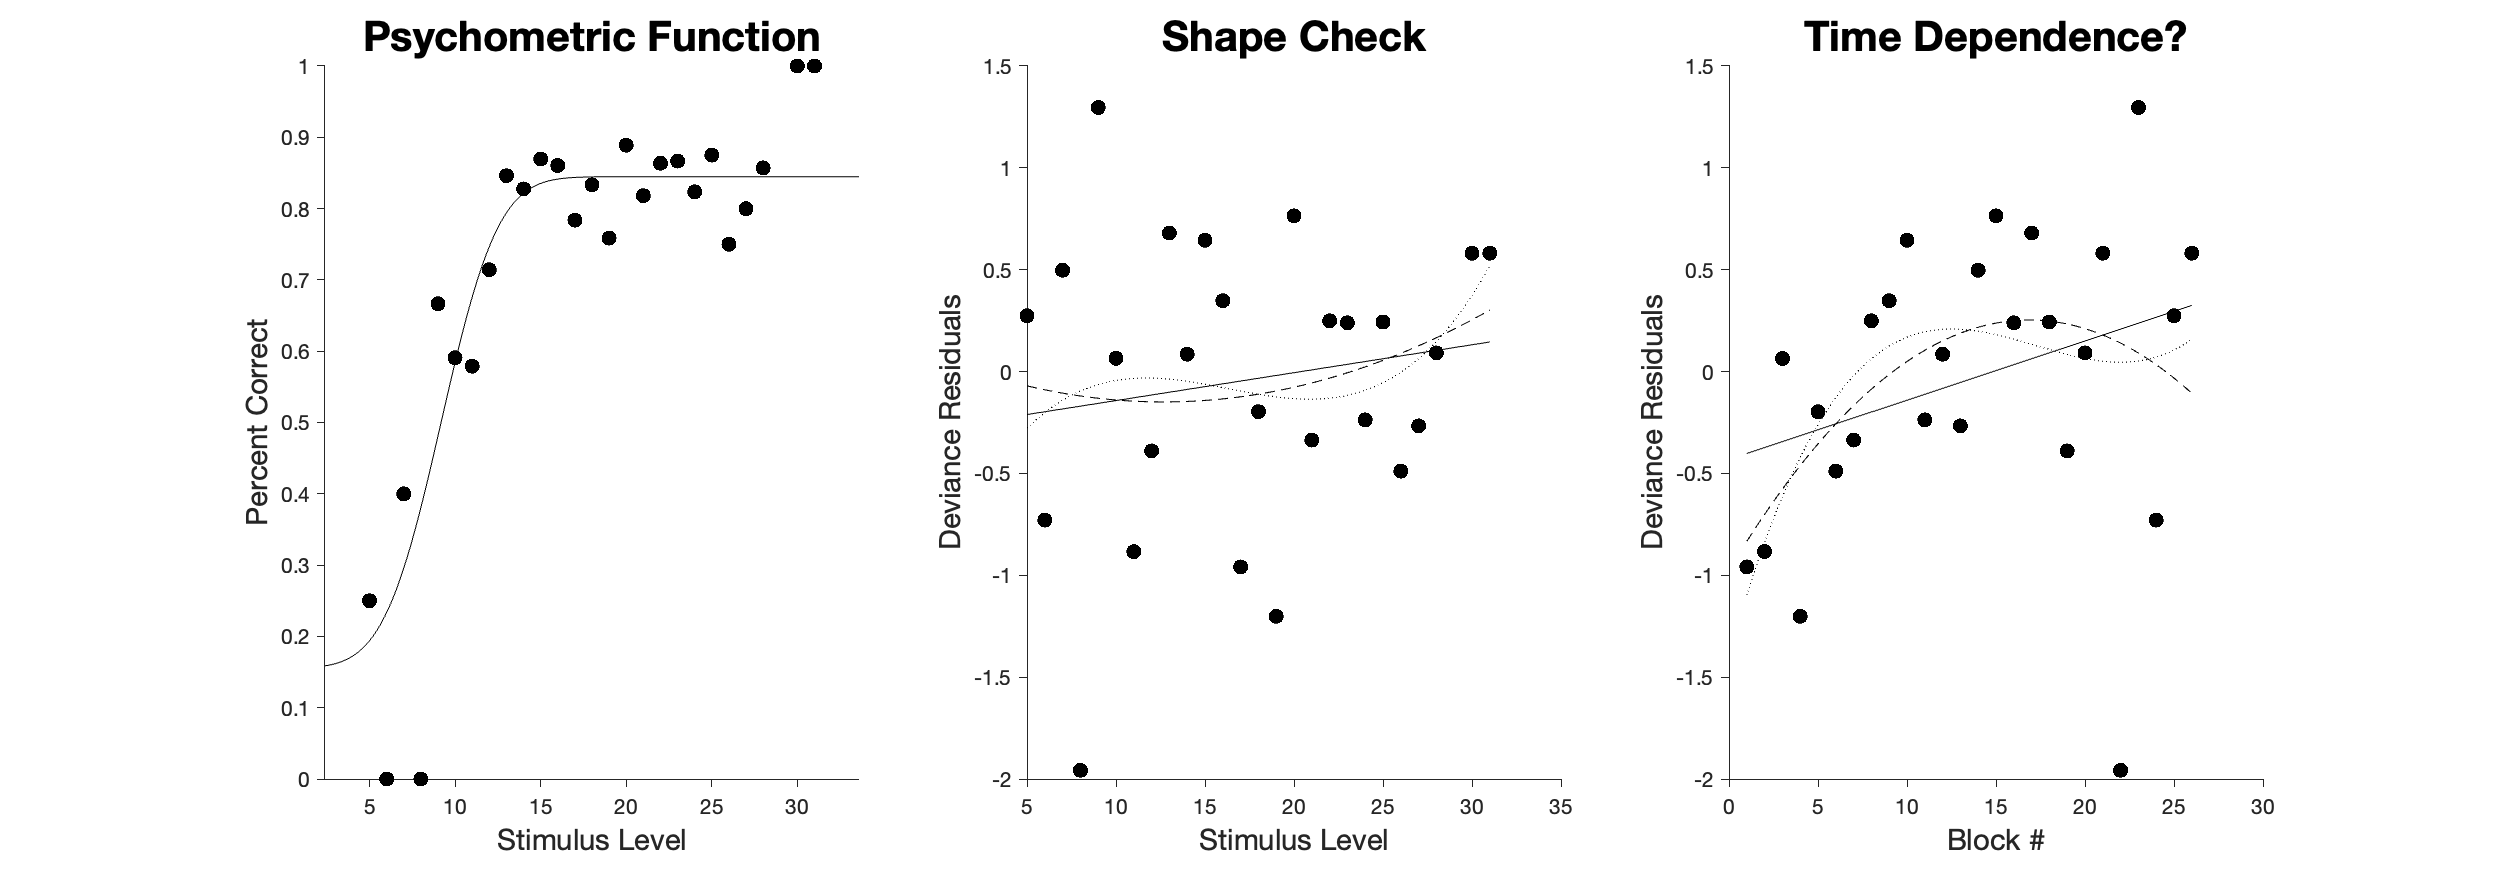
\includegraphics[width = \linewidth]{Thesis/plots/gof/segSize/segSize_da_short_deviance.png}
        \caption{Deviance residuals for short exposure time}
    \end{subfigure}
    \begin{subfigure}{\textwidth}
        \centering
        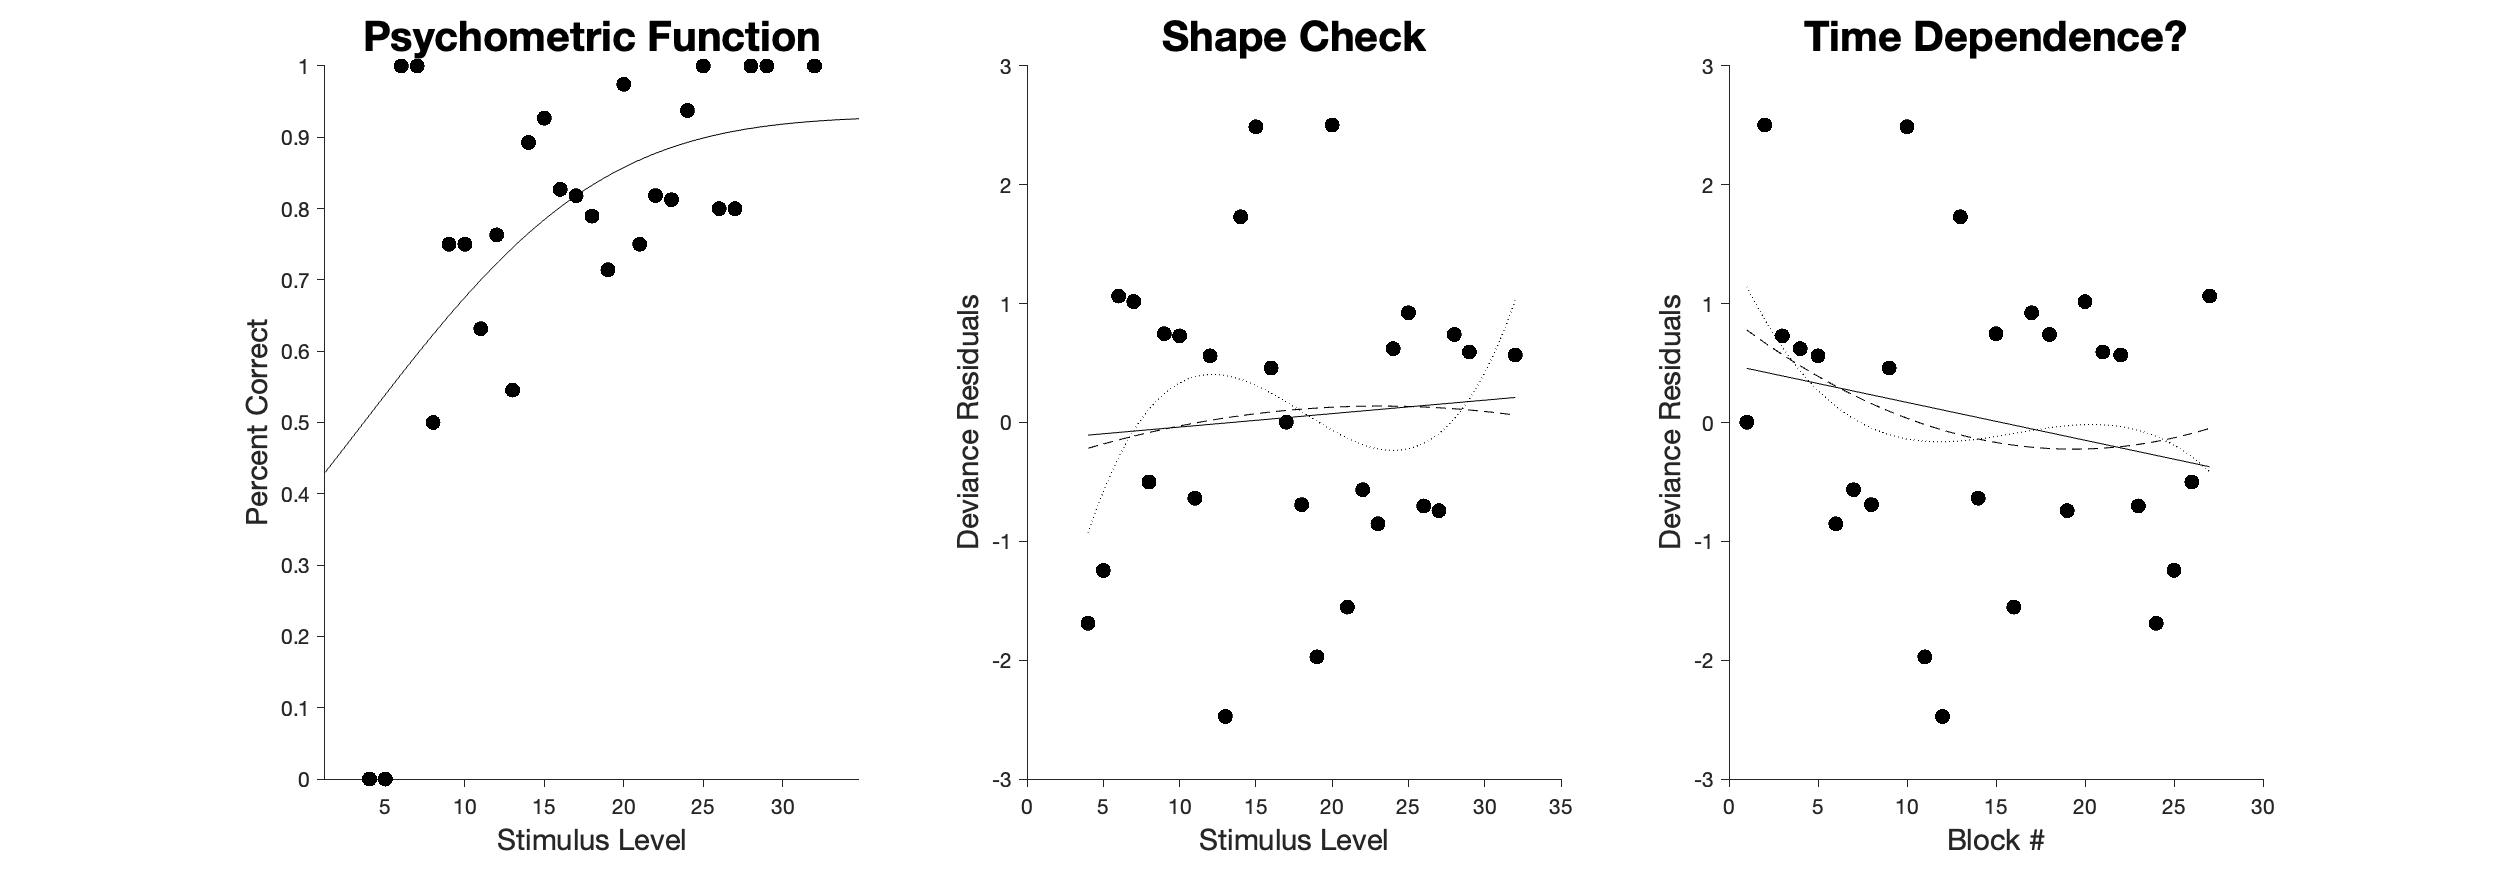
\includegraphics[width = \linewidth]{Thesis/plots/gof/segSize/segSize_da_long_deviance.png}
        \caption{Deviance residuals for long exposure time}
    \end{subfigure}
\end{figure}

\clearpage

\subsubsection*{J.S.}
\begin{figure}[!hb]
    \begin{subfigure}{0.494\textwidth}
        \centering
        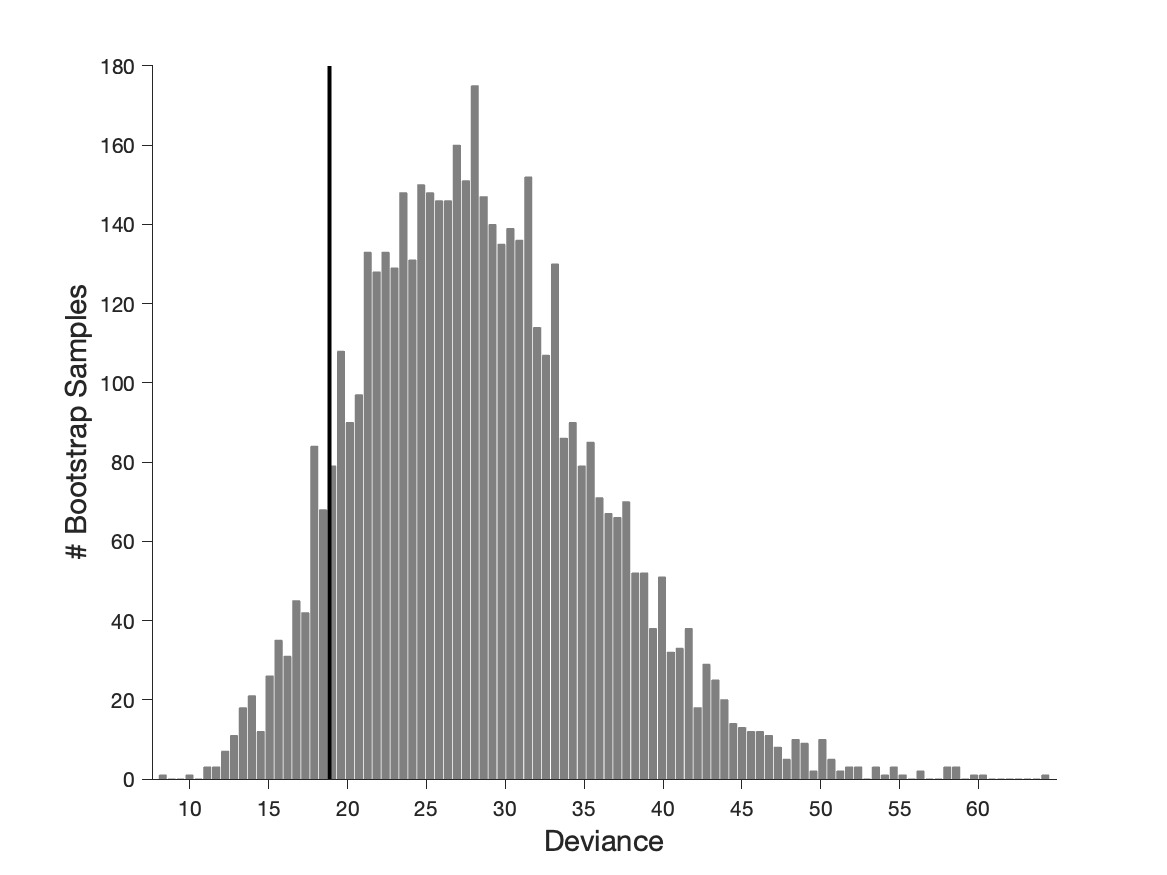
\includegraphics[width = \linewidth]{Thesis/plots/gof/segSize/segSize_js_short_bootstrap.png}
        \caption{Monte-Carlo generated deviance histograms for short exposure time}
        \label{fig:da_gof_short_bootstrap}
    \end{subfigure}
    \hspace{0.01\textwidth}
    \begin{subfigure}{0.494\textwidth}
        \centering
        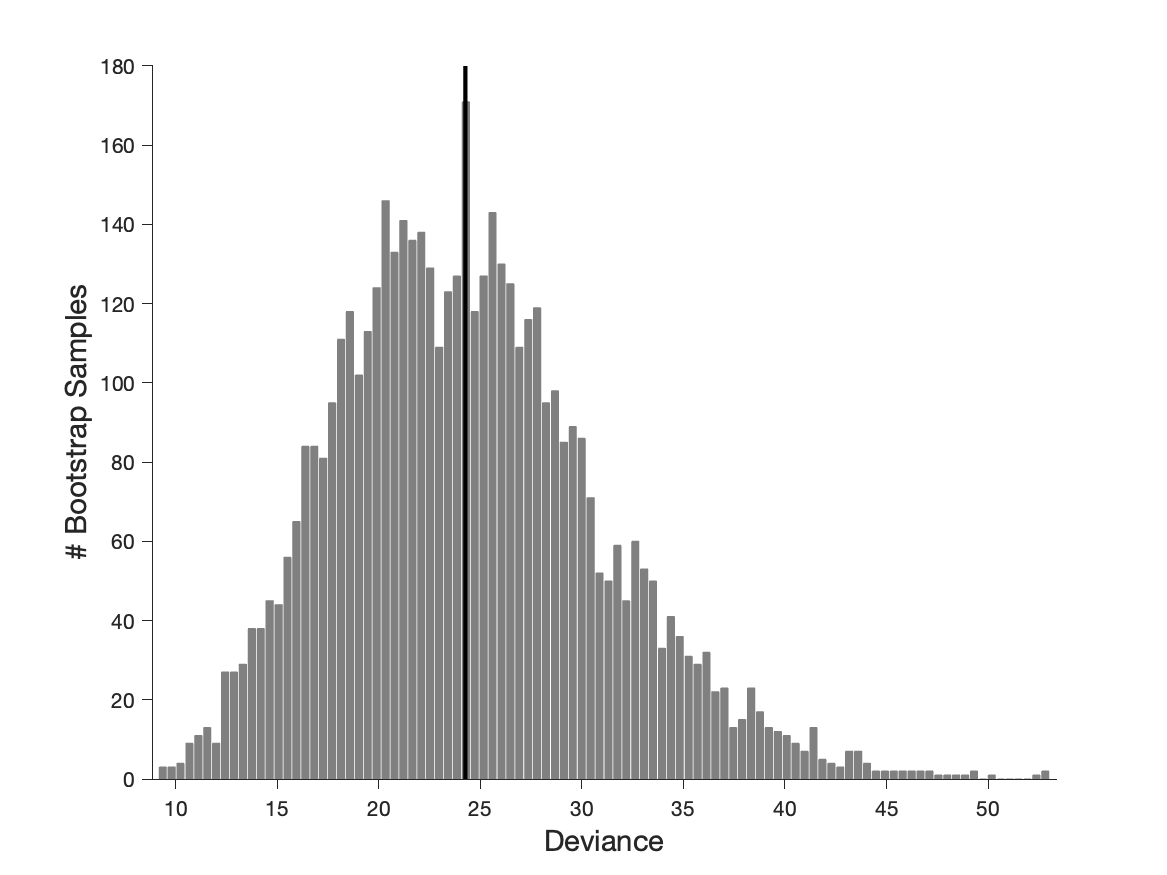
\includegraphics[width = \linewidth]{Thesis/plots/gof/segSize/segSize_js_long_bootstrap.png}
        \caption{Monte-Carlo generated deviance histograms for long exposure time}
        \label{fig:da_gof_long_bootstrap}
    \end{subfigure}
    
    \begin{subfigure}{\textwidth}
        \centering
        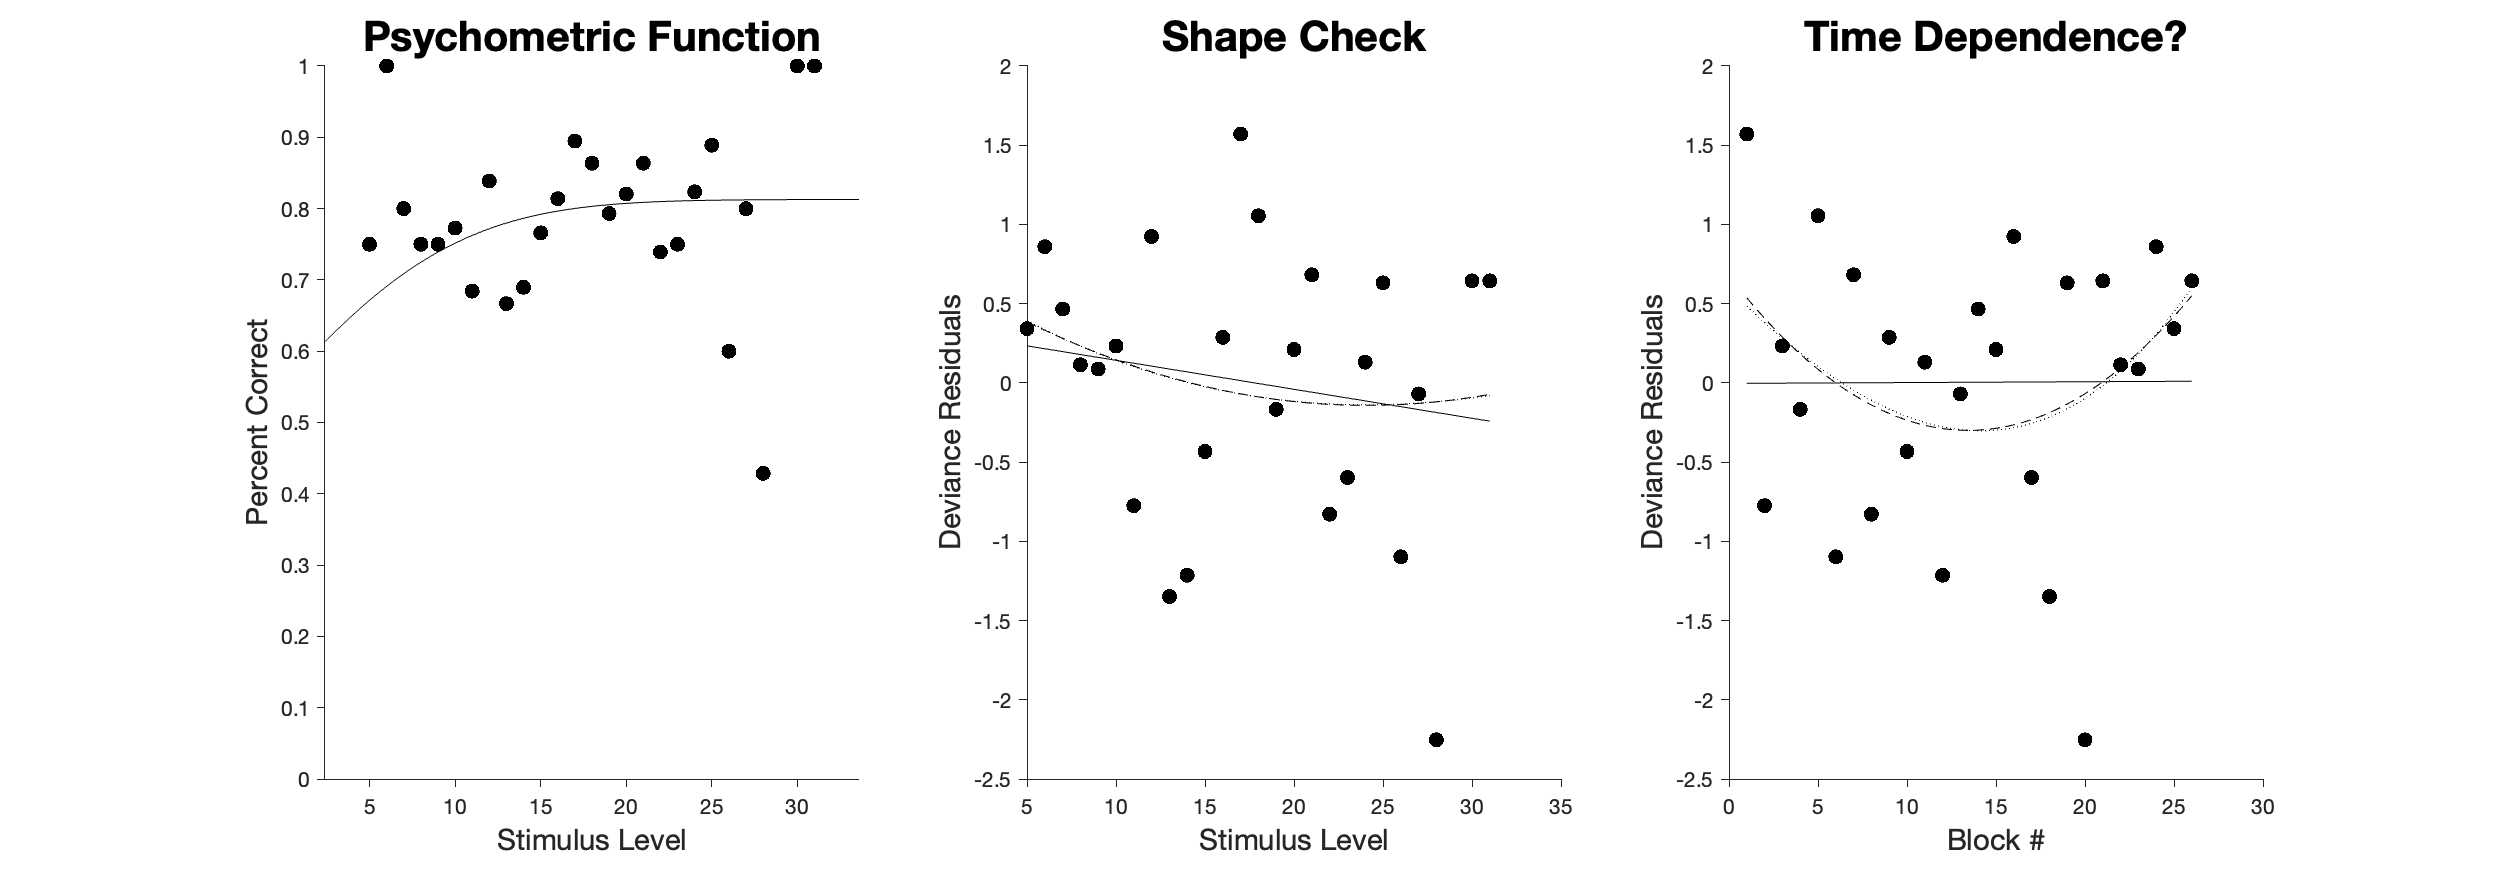
\includegraphics[width = \linewidth]{Thesis/plots/gof/segSize/segSize_js_short_deviance.png}
        \caption{Monte-Carlo generated deviance histograms for short exposure time}
    \end{subfigure}
    \begin{subfigure}{\textwidth}
        \centering
        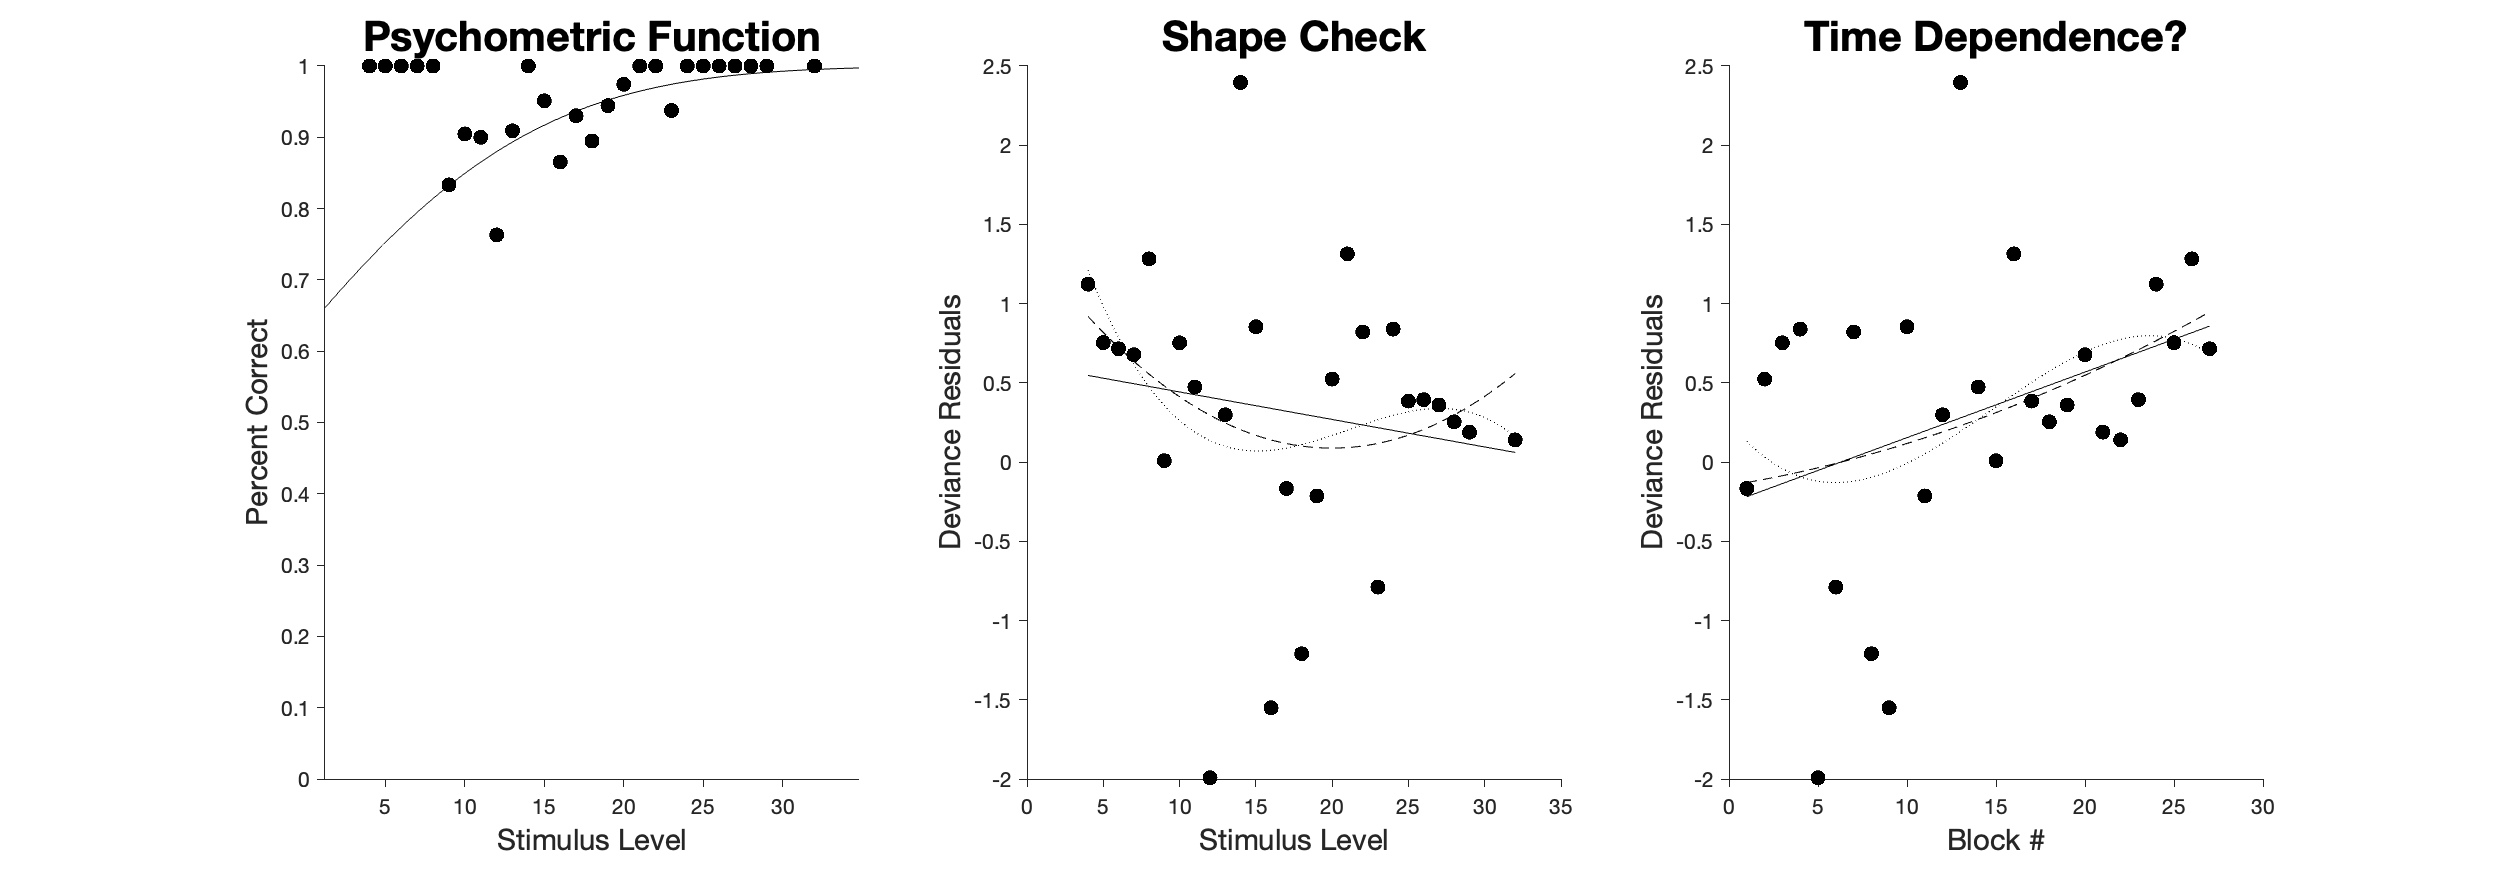
\includegraphics[width = \linewidth]{Thesis/plots/gof/segSize/segSize_js_long_deviance.png}
        \caption{Monte-Carlo generated deviance histograms for long exposure time}
    \end{subfigure}
\end{figure}

\clearpage

\subsection{Segment Distance}

\subsubsection*{E.B.}
\begin{figure}[!hb]
    \begin{subfigure}{0.494\textwidth}
        \centering
        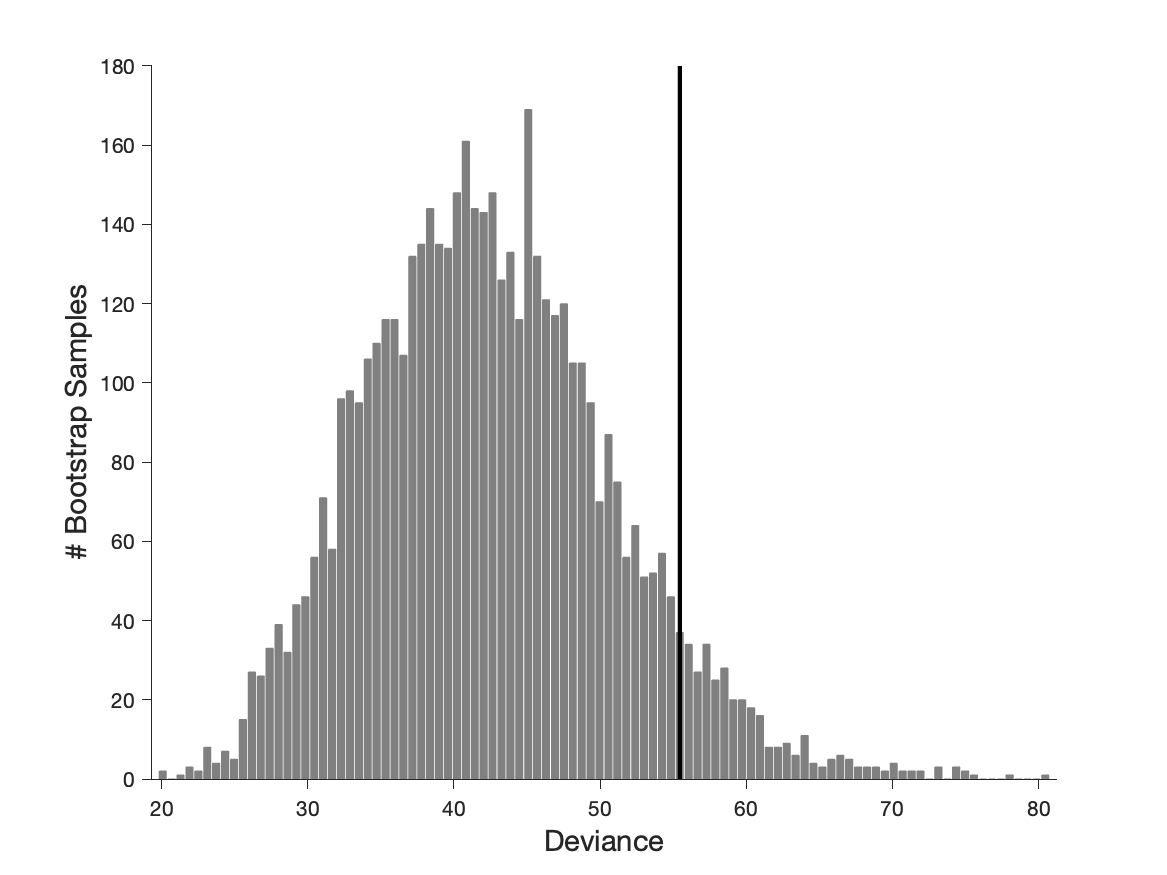
\includegraphics[width = \linewidth]{Thesis/plots/gof/segDist/segDist_eb_short_bootstrap.png}
        \caption{Monte-Carlo generated deviance histograms for short exposure time}
        \label{fig:da_gof_short_bootstrap}
    \end{subfigure}
    \hspace{0.01\textwidth}
    \begin{subfigure}{0.494\textwidth}
        \centering
        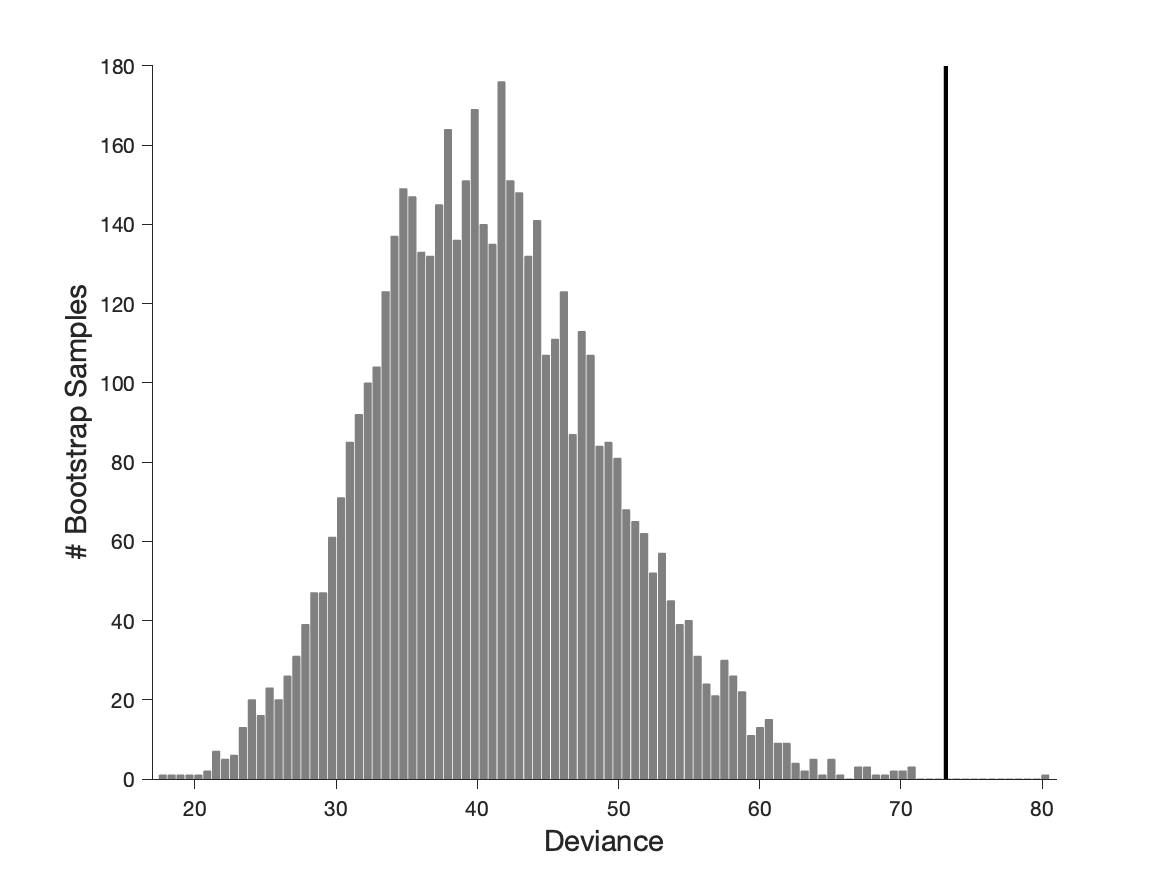
\includegraphics[width = \linewidth]{Thesis/plots/gof/segDist/segDist_eb_long_bootstrap.png}
        \caption{Monte-Carlo generated deviance histograms for long exposure time}
        \label{fig:da_gof_long_bootstrap}
    \end{subfigure}
    
    \begin{subfigure}{\textwidth}
        \centering
        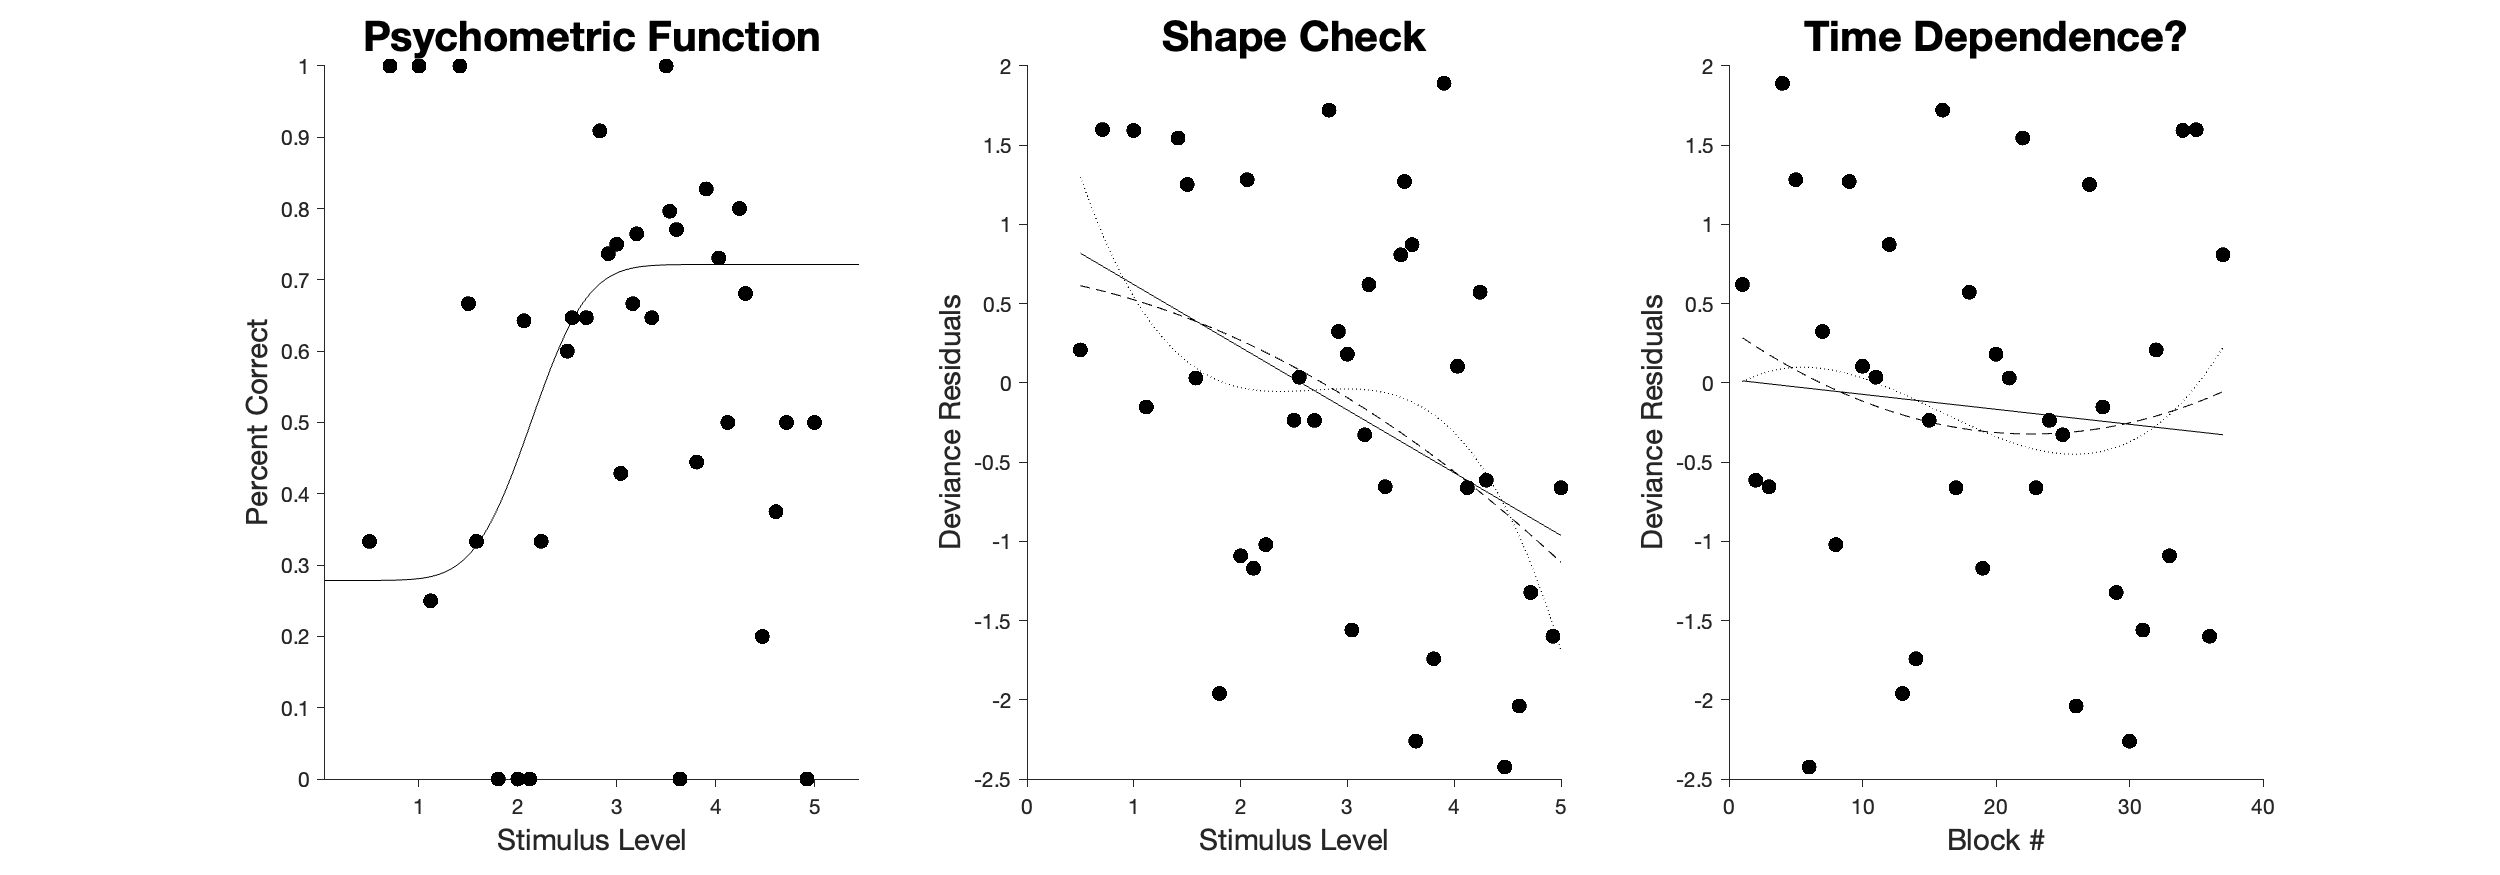
\includegraphics[width = \linewidth]{Thesis/plots/gof/segDist/segDist_eb_short_deviance.png}
        \caption{Deviance residuals for short exposure time}
    \end{subfigure}
    
    \begin{subfigure}{\textwidth}
        \centering
        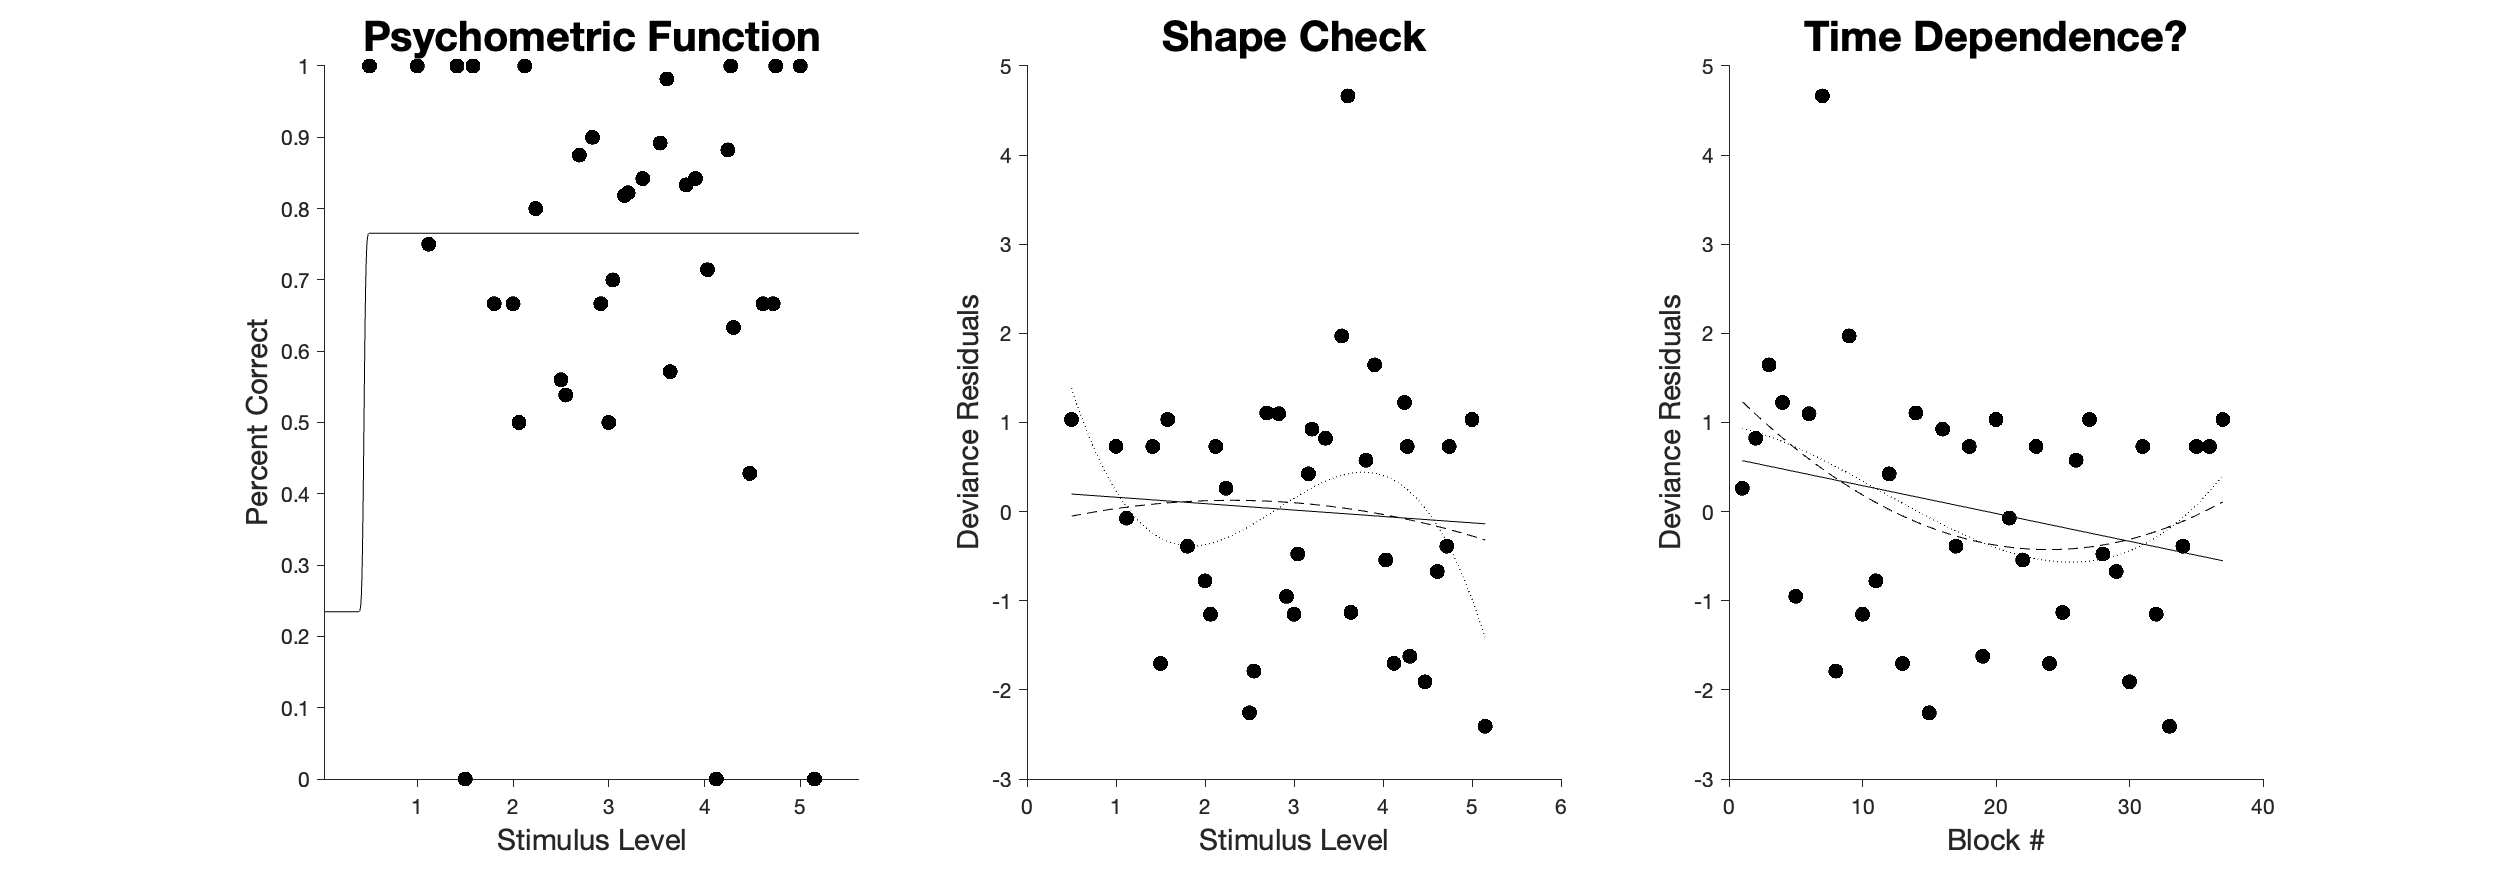
\includegraphics[width = \linewidth]{Thesis/plots/gof/segDist/segDist_eb_long_deviance.png}
        \caption{Deviance residuals for long exposure time}
    \end{subfigure}
\end{figure}

\clearpage

\subsubsection*{G.O.}
\begin{figure}[!hb]
    \begin{subfigure}{0.494\textwidth}
        \centering
        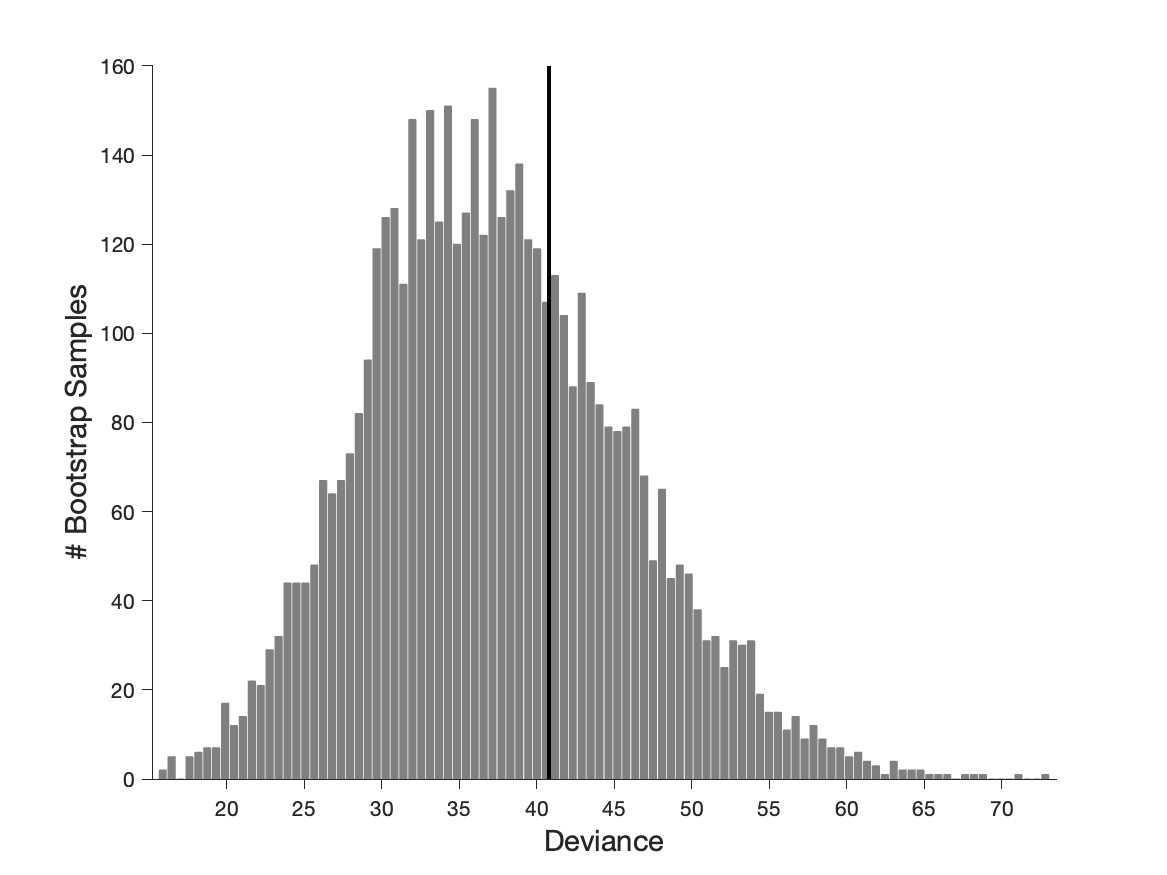
\includegraphics[width = \linewidth]{Thesis/plots/gof/segDist/segDist_go_short_bootstrap.png}
        \caption{Monte-Carlo generated deviance histograms for short exposure time}
        \label{fig:da_gof_short_bootstrap}
    \end{subfigure}
    \hspace{0.01\textwidth}
    \begin{subfigure}{0.494\textwidth}
        \centering
        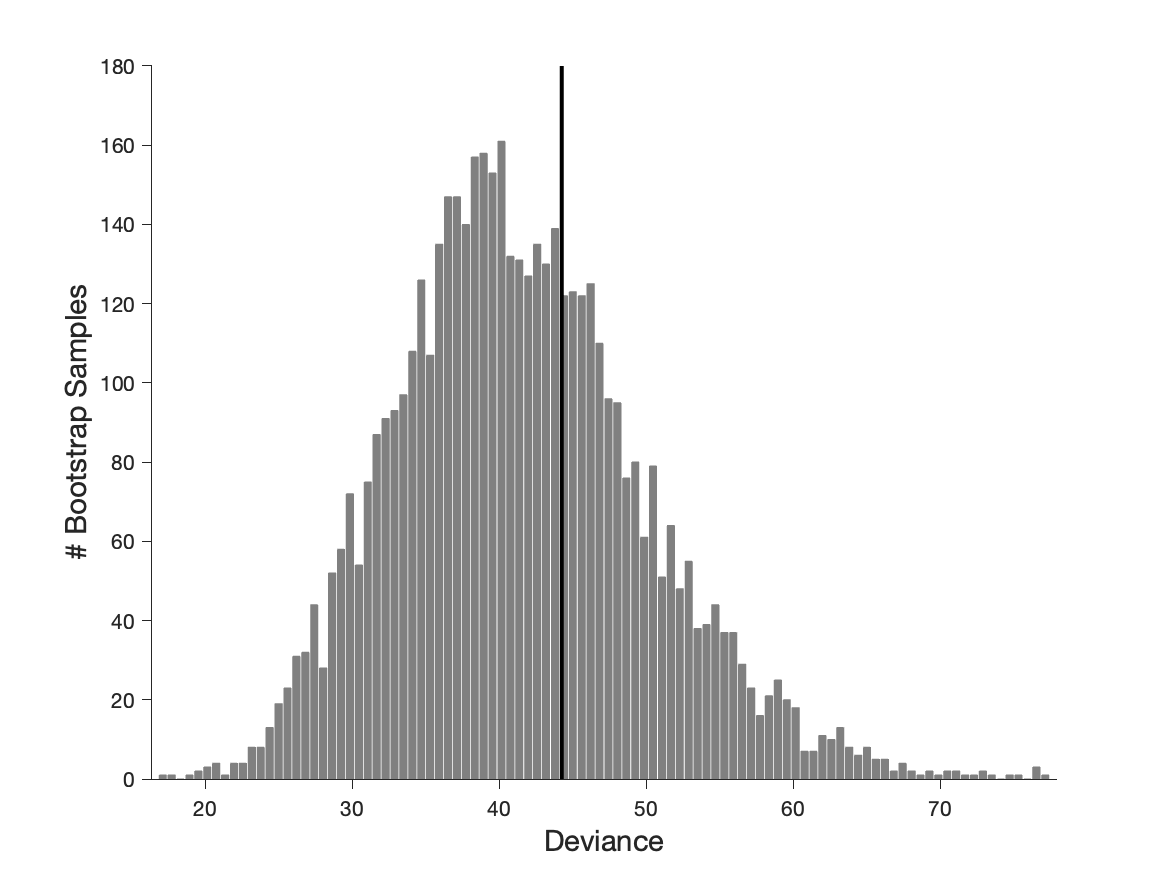
\includegraphics[width = \linewidth]{Thesis/plots/gof/segDist/segDist_go_long_bootstrap.png}
        \caption{Monte-Carlo generated deviance histograms for long exposure time}
        \label{fig:da_gof_long_bootstrap}
    \end{subfigure}
    
    \begin{subfigure}{\textwidth}
        \centering
        \includegraphics[width = \linewidth]{Thesis/plots/gof/segDist/segDist_go_short_deviance.png}
        \caption{Deviance residuals for short exposure time}
    \end{subfigure}
    
    \begin{subfigure}{\textwidth}
        \centering
        \includegraphics[width = \linewidth]{Thesis/plots/gof/segDist/segDist_go_long_deviance.png}
        \caption{Deviance residuals for long exposure time}
    \end{subfigure}
    
\end{figure}
\clearpage

\subsubsection*{M.A.E.}
\begin{figure}[!hb]
    \begin{subfigure}{0.494\textwidth}
        \centering
        \includegraphics[width = \linewidth]{Thesis/plots/gof/segDist/segDist_mae_short_bootstrap.png}
        \caption{Monte-Carlo generated deviance histograms for short exposure time}
        \label{fig:da_gof_short_bootstrap}
    \end{subfigure}
    \hspace{0.01\textwidth}
    \begin{subfigure}{0.494\textwidth}
        \centering
        \includegraphics[width = \linewidth]{Thesis/plots/gof/segDist/segDist_mae_long_bootstrap.png}
        \caption{Monte-Carlo generated deviance histograms for long exposure time}
        \label{fig:da_gof_long_bootstrap}
    \end{subfigure}
    
    \begin{subfigure}{\textwidth}
        \centering
        \includegraphics[width = \linewidth]{Thesis/plots/gof/segDist/segDist_mae_short_deviance.png}
        \caption{Deviance residuals for short exposure time}
    \end{subfigure}
    \begin{subfigure}{\textwidth}
        \centering
        \includegraphics[width = \linewidth]{Thesis/plots/gof/segDist/segDist_mae_long_deviance.png}
        \caption{Deviance residuals for long exposure time}
    \end{subfigure}
\end{figure}

\clearpage

\subsubsection*{R.E.}
\begin{figure}[!hb]
    \begin{subfigure}{0.494\textwidth}
        \centering
        \includegraphics[width = \linewidth]{Thesis/plots/gof/segDist/segDist_re_short_bootstrap.png}
        \caption{Monte-Carlo generated deviance histograms for short exposure time}
        \label{fig:da_gof_short_bootstrap}
    \end{subfigure}
    \hspace{0.01\textwidth}
    \begin{subfigure}{0.494\textwidth}
        \centering
        \includegraphics[width = \linewidth]{Thesis/plots/gof/segDist/segDist_re_long_bootstrap.png}
        \caption{Monte-Carlo generated deviance histograms for long exposure time}
        \label{fig:da_gof_long_bootstrap}
    \end{subfigure}
    
    \begin{subfigure}{\textwidth}
        \centering
        \includegraphics[width = \linewidth]{Thesis/plots/gof/segDist/segDist_re_short_deviance.png}
        \caption{Deviance residuals for short exposure time}
    \end{subfigure}
    
    \begin{subfigure}{\textwidth}
        \centering
        \includegraphics[width = \linewidth]{Thesis/plots/gof/segDist/segDist_re_long_deviance.png}
        \caption{Deviance residuals for long exposure time}
    \end{subfigure}
\end{figure}

\clearpage

\subsubsection*{D.A.}
\begin{figure}[!hb]
    \begin{subfigure}{0.494\textwidth}
        \centering
        \includegraphics[width = \linewidth]{Thesis/plots/gof/segDist/segDist_da_short_bootstrap.png}
        \caption{Monte-Carlo generated deviance histograms for short exposure time}
        \label{fig:da_gof_short_bootstrap}
    \end{subfigure}
    \hspace{0.01\textwidth}
    \begin{subfigure}{0.494\textwidth}
        \centering
        \includegraphics[width = \linewidth]{Thesis/plots/gof/segDist/segDist_da_long_bootstrap.png}
        \caption{Monte-Carlo generated deviance histograms for long exposure time}
        \label{fig:da_gof_long_bootstrap}
    \end{subfigure}
    
    \begin{subfigure}{\textwidth}
        \centering
        \includegraphics[width = \linewidth]{Thesis/plots/gof/segDist/segDist_da_short_deviance.png}
        \caption{Deviance residuals for short exposure time}
    \end{subfigure}
    \begin{subfigure}{\textwidth}
        \centering
        \includegraphics[width = \linewidth]{Thesis/plots/gof/segDist/segDist_da_long_deviance.png}
        \caption{Deviance residuals for long exposure time}
    \end{subfigure}
\end{figure}

\clearpage

\subsubsection*{J.S.}
\begin{figure}[!hb]
    \begin{subfigure}{0.494\textwidth}
        \centering
        \includegraphics[width = \linewidth]{Thesis/plots/gof/segDist/segDist_js_short_bootstrap.png}
        \caption{Monte-Carlo generated deviance histograms for short exposure time}
        \label{fig:da_gof_short_bootstrap}
    \end{subfigure}
    \hspace{0.01\textwidth}
    \begin{subfigure}{0.494\textwidth}
        \centering
        \includegraphics[width = \linewidth]{Thesis/plots/gof/segDist/segDist_js_long_bootstrap.png}
        \caption{Monte-Carlo generated deviance histograms for long exposure time}
        \label{fig:da_gof_long_bootstrap}
    \end{subfigure}
    
    \begin{subfigure}{\textwidth}
        \centering
        \includegraphics[width = \linewidth]{Thesis/plots/gof/segDist/segDist_js_short_deviance.png}
        \caption{Monte-Carlo generated deviance histograms for short exposure time}
    \end{subfigure}
    \begin{subfigure}{\textwidth}
        \centering
        \includegraphics[width = \linewidth]{Thesis/plots/gof/segDist/segDist_js_long_deviance.png}
        \caption{Monte-Carlo generated deviance histograms for long exposure time}
    \end{subfigure}
\end{figure}

\clearpage

\subsection{Cut No}

\subsubsection*{E.B.}
\begin{figure}[!hb]
    \begin{subfigure}{0.494\textwidth}
        \centering
        \includegraphics[width = \linewidth]{Thesis/plots/gof/cutNo/cutNo_eb_short_bootstrap.png}
        \caption{Monte-Carlo generated deviance histograms for short exposure time}
        \label{fig:da_gof_short_bootstrap}
    \end{subfigure}
    \hspace{0.01\textwidth}
    \begin{subfigure}{0.494\textwidth}
        \centering
        \includegraphics[width = \linewidth]{Thesis/plots/gof/cutNo/cutNo_eb_long_bootstrap.png}
        \caption{Monte-Carlo generated deviance histograms for long exposure time}
        \label{fig:da_gof_long_bootstrap}
    \end{subfigure}
    
    \begin{subfigure}{\textwidth}
        \centering
        \includegraphics[width = \linewidth]{Thesis/plots/gof/cutNo/cutNo_eb_short_deviance.png}
        \caption{Deviance residuals for short exposure time}
    \end{subfigure}
    
    \begin{subfigure}{\textwidth}
        \centering
        \includegraphics[width = \linewidth]{Thesis/plots/gof/cutNo/cutNo_eb_long_deviance.png}
        \caption{Deviance residuals for long exposure time}
    \end{subfigure}
\end{figure}

\clearpage

\subsubsection*{G.O.}
\begin{figure}[!hb]
    \begin{subfigure}{0.494\textwidth}
        \centering
        \includegraphics[width = \linewidth]{Thesis/plots/gof/cutNo/cutNo_go_short_bootstrap.png}
        \caption{Monte-Carlo generated deviance histograms for short exposure time}
        \label{fig:da_gof_short_bootstrap}
    \end{subfigure}
    \hspace{0.01\textwidth}
    \begin{subfigure}{0.494\textwidth}
        \centering
        \includegraphics[width = \linewidth]{Thesis/plots/gof/cutNo/cutNo_go_long_bootstrap.png}
        \caption{Monte-Carlo generated deviance histograms for long exposure time}
        \label{fig:da_gof_long_bootstrap}
    \end{subfigure}
    
    \begin{subfigure}{\textwidth}
        \centering
        \includegraphics[width = \linewidth]{Thesis/plots/gof/cutNo/cutNo_go_short_deviance.png}
        \caption{Deviance residuals for short exposure time}
    \end{subfigure}
    
    \begin{subfigure}{\textwidth}
        \centering
        \includegraphics[width = \linewidth]{Thesis/plots/gof/cutNo/cutNo_go_long_deviance.png}
        \caption{Deviance residuals for long exposure time}
    \end{subfigure}
    
\end{figure}
\clearpage

\subsubsection*{M.A.E.}
\begin{figure}[!hb]
    \begin{subfigure}{0.494\textwidth}
        \centering
        \includegraphics[width = \linewidth]{Thesis/plots/gof/cutNo/cutNo_mae_short_bootstrap.png}
        \caption{Monte-Carlo generated deviance histograms for short exposure time}
        \label{fig:da_gof_short_bootstrap}
    \end{subfigure}
    \hspace{0.01\textwidth}
    \begin{subfigure}{0.494\textwidth}
        \centering
        \includegraphics[width = \linewidth]{Thesis/plots/gof/cutNo/cutNo_mae_long_bootstrap.png}
        \caption{Monte-Carlo generated deviance histograms for long exposure time}
        \label{fig:da_gof_long_bootstrap}
    \end{subfigure}
    
    \begin{subfigure}{\textwidth}
        \centering
        \includegraphics[width = \linewidth]{Thesis/plots/gof/cutNo/cutNo_mae_short_deviance.png}
        \caption{Deviance residuals for short exposure time}
    \end{subfigure}
    \begin{subfigure}{\textwidth}
        \centering
        \includegraphics[width = \linewidth]{Thesis/plots/gof/cutNo/cutNo_mae_long_deviance.png}
        \caption{Deviance residuals for long exposure time}
    \end{subfigure}
\end{figure}

\clearpage

\subsubsection*{R.E.}
\begin{figure}[!hb]
    \begin{subfigure}{0.494\textwidth}
        \centering
        \includegraphics[width = \linewidth]{Thesis/plots/gof/cutNo/cutNo_re_short_bootstrap.png}
        \caption{Monte-Carlo generated deviance histograms for short exposure time}
        \label{fig:da_gof_short_bootstrap}
    \end{subfigure}
    \hspace{0.01\textwidth}
    \begin{subfigure}{0.494\textwidth}
        \centering
        \includegraphics[width = \linewidth]{Thesis/plots/gof/cutNo/cutNo_re_long_bootstrap.png}
        \caption{Monte-Carlo generated deviance histograms for long exposure time}
        \label{fig:da_gof_long_bootstrap}
    \end{subfigure}
    
    \begin{subfigure}{\textwidth}
        \centering
        \includegraphics[width = \linewidth]{Thesis/plots/gof/cutNo/cutNo_re_short_deviance.png}
        \caption{Deviance residuals for short exposure time}
    \end{subfigure}
    
    \begin{subfigure}{\textwidth}
        \centering
        \includegraphics[width = \linewidth]{Thesis/plots/gof/cutNo/cutNo_re_long_deviance.png}
        \caption{Deviance residuals for long exposure time}
    \end{subfigure}
\end{figure}

\clearpage

\subsubsection*{D.A.}
\begin{figure}[!hb]
    \begin{subfigure}{0.494\textwidth}
        \centering
        \includegraphics[width = \linewidth]{Thesis/plots/gof/cutNo/cutNo_da_short_bootstrap.png}
        \caption{Monte-Carlo generated deviance histograms for short exposure time}
        \label{fig:da_gof_short_bootstrap}
    \end{subfigure}
    \hspace{0.01\textwidth}
    \begin{subfigure}{0.494\textwidth}
        \centering
        \includegraphics[width = \linewidth]{Thesis/plots/gof/cutNo/cutNo_da_long_bootstrap.png}
        \caption{Monte-Carlo generated deviance histograms for long exposure time}
        \label{fig:da_gof_long_bootstrap}
    \end{subfigure}
    
    \begin{subfigure}{\textwidth}
        \centering
        \includegraphics[width = \linewidth]{Thesis/plots/gof/cutNo/cutNo_da_short_deviance.png}
        \caption{Deviance residuals for short exposure time}
    \end{subfigure}
    \begin{subfigure}{\textwidth}
        \centering
        \includegraphics[width = \linewidth]{Thesis/plots/gof/cutNo/cutNo_da_long_deviance.png}
        \caption{Deviance residuals for long exposure time}
    \end{subfigure}
\end{figure}

\clearpage

\subsubsection*{J.S.}
\begin{figure}[!hb]
    \begin{subfigure}{0.494\linewidth}
        \centering
        \includegraphics[width = \linewidth]{Thesis/plots/gof/cutNo/cutNo_js_short_bootstrap.png}
        \caption{Monte-Carlo generated deviance histograms for short exposure time}
        \label{fig:da_gof_short_bootstrap}
    \end{subfigure}
    \hspace{0.01\textwidth}
    \begin{subfigure}{0.494\linewidth}
        \centering
        \includegraphics[width = \linewidth]{Thesis/plots/gof/cutNo/cutNo_js_long_bootstrap.png}
        \caption{Monte-Carlo generated deviance histograms for long exposure time}
        \label{fig:da_gof_long_bootstrap}
    \end{subfigure}
    
    \begin{subfigure}{\linewidth}
        \centering
        \includegraphics[width=1.3\linewidth]{Thesis/plots/gof/cutNo/cutNo_js_short_deviance.png}
        \caption{Monte-Carlo generated deviance histograms for short exposure time}
    \end{subfigure}
    \begin{subfigure}{\linewidth}
        \centering
        \includegraphics[width=1.3\linewidth]{Thesis/plots/gof/segDist/segDist_js_long_deviance.png}
        \caption{Monte-Carlo generated deviance histograms for long exposure time}
    \end{subfigure}
    
\end{figure}

\clearpage

\section{Predicting key presses}
\textbf{Mixed Effect Regression Results on key presses.} In order to test if participants think that they saw the target segment in the presented image, we used segment distance, segment size, and trial type as predictors. Since yes key presses are coded as 0 and no presses as 1, negative coefficients suggest that participants pressed yes keys more as the segment size and distance increases. Additionally, in the control trials when the segment was located further to the center, they pressed yes key more. 
\label{table:keyPress}    
\begin{table}[ht]
\centering
\begin{tabular}{rrrrr}
  \hline
 & Estimate & Std. Error & z value & Pr($>$$|$z$|$) \\ 
  \hline
(Intercept) & 0.29 & 0.02 & 12.10 & 0.00 \\ 
  Test Trial:Segment Distance & -0.93 & 0.03 & -27.30 & 0.00 \\ 
  Control Trial:Segment Distance & -0.43 & 0.03 & -14.44 & 0.00 \\ 
  Control Trial:Segment Size & -0.80 & 0.03 & -26.22 & 0.00 \\ 
  Test Trial:Segment Size & -0.60 & 0.03 & -18.33 & 0.00 \\ 
   \hline
\end{tabular}
\end{table}

\end{document}